% Ce fichier main.tex est le fichier principal \`{a} partir duquel tout est g\'{e}n\'{e}r\'{e}
% This file is the main file where the final document is generated
\documentclass[table]{these-dbl}
% Remplir les metadonnees du pdf
% Fill the pdf metadata

\hypersetup{
%    pdfauthor   = {XYZ},
%    pdftitle    = {Th\`{e}se de doctorat de XYZ},
%    pdfsubject  = {Th\`{e}se de doctorat de XYZ},
%    pdfkeywords = {mots-cl\'{e}s},
}

\geometry{vmargin=4.0cm}

% Spécifier vos fichiers de bibliographie
% Specify you bibliography files here
\addbibresource{./biblio/biblio.bib}
%\usepackage[table]{xcolor}
%\bibliography{./biblio/biblio.bib}
\usepackage[ruled,vlined,linesnumbered,algo2e]{algorithm2e} 
%\usepackage{xcolor}
\usepackage{amsmath,amssymb,amsfonts}

\newcommand{\ie}{\emph{i.e.,}\xspace}
\newcommand{\eg}{\emph{e.g.,}\xspace}
\newcommand{\cf}{\emph{cf.}\xspace}
\newcommand{\etal}{\emph{et al.}\xspace}
\newcommand{\etc}{\emph{etc.}\xspace}
\usepackage{booktabs}
\usepackage{multirow}
\usepackage{xurl}

\usepackage{hhline}
\newcommand{\blue}[1]{{#1}}
\newcommand{\green}[1]{{\color{teal}{#1}}}
\newcommand{\red}[1]{{#1}}


\usepackage{ragged2e}
\definecolor{CellColor1}{rgb}{1,1,0.82}
\begin{document}
	
%\newcommand{\red}[1]{{\color{red}{#1}}}

% Page de garde avec commande \maketitle
% Front cover calling \maketitle
% La page de garde est en français
% The front cover is in French
\selectlanguage{french}

% Inclure les infos de chaque établissement
% Include each institution data

%%% Switch case in latex
%%% https://tex.stackexchange.com/a/343306
\makeatletter
\newcommand\addcase[3]{\expandafter\def\csname\string#1@case@#2\endcsname{#3}}
\newcommand\makeswitch[2][]{%
    \newcommand#2[1]{%
        \ifcsname\string#2@case@##1\endcsname\csname\string#2@case@##1\endcsname\else#1\fi%
  }%
}
\makeatother

%%%% Il faut adapter la taille des logos dans certains cas (e.g., EGAAL, 2 etablissements)
\newcommand\hauteurlogos[3]{
    \hauteurlogoecole{#1}
    \hauteurlogoetablissementA{#2}
    \hauteurlogoetablissementB{#3}
}





%%%%%%%%%%%%%%%%%%%%%%%%%%%%%%%%%%%%%%%%%%%%%%%%%%%
%%%%%%%%%%%%%%%% ECOLES DOCTORALES %%%%%%%%%%%%%%%%

%%%% #1: dossier des images, #2: numero ED, #3: couleur ED recto, #4: couleur ED verso, #5-#6: nom complet sur plusieurs lignes
\newcommand\addecoledoctorale[6]{
    \direcole{#1}
    \numeroecole{#2}
    \definecolor{couleur-ecole-recto}{RGB}{#3}
    \definecolor{couleur-ecole-verso}{RGB}{#4}
    \nomecoleA{#5}
    \nomecoleB{#6}
}

\makeswitch[default]\ecoledoctorale{}

\addcase\ecoledoctorale{ALL}{\addecoledoctorale
    {ALL}
    {595}
    {255,165,139}
    {232,86,18}
    {Arts, Lettres, Langues}
    {}
}
\addcase\ecoledoctorale{DSP}{\addecoledoctorale
    {DSP}
    {599}
    {255,241,170}
    {255,214,12}
    {Droit et Science politiques}
    {}
}
\addcase\ecoledoctorale{EDGE}{\addecoledoctorale
    {EDGE}
    {597}
    {255,254,101}
    {255,237,0}
    {Sciences \'{e}conomiques et sciences de gestion - Bretagne}
    {}
}
\addcase\ecoledoctorale{EGAAL}{\addecoledoctorale
    {EGAAL}
    {600}
    {0,118,0}
    {0,93,49}
    {\'{E}cologie, G\'{e}osciences, Agronomie, Alimentation}
    {}
    \couleurpolice{white}
}
\addcase\ecoledoctorale{ELICCE}{\addecoledoctorale
    {ELICCE}
    {646}
    {255,207,114}
    {252,199,82}
    {\'{E}ducation, Langages, Interactions, Cognition, Clinique, Expertise}
    {}
}
\addcase\ecoledoctorale{ESC}{\addecoledoctorale
    {ESC}
    {645}
    {255,164,85}
    {240,138,0}
    {Espaces, Soci\'{e}\'{e}s, Civilisations}
    {}
}
\addcase\ecoledoctorale{MathSTICBO}{\addecoledoctorale
    {MathSTICBO}
    {644}
    {190,212,233}
    {139,181,221}
    {Math\'{e}matiques et Sciences et Technologies}
    {de l'Information et de la Communication en Bretagne Oc\'{e}ane}
}
\addcase\ecoledoctorale{MATISSE}{\addecoledoctorale
    {MATISSE}
    {601}
    {0,112,237}
    {0,84,160}
    {Math\'{e}matiques, T\'{e}l\'{e}communications, Informatique, Signal, Syst\`{e}mes,}
    {\'{E}lectronique}
    \hauteurlogos{1.8cm}{1.8cm}{1.8cm}
    \couleurpolice{white}
}
\addcase\ecoledoctorale{S3M}{\addecoledoctorale
    {S3M}
    {638}
    {159,19,90}
    {156,42,100}
    {Sciences de la Mati\`{e}re, des Mol\'{e}cules et Mat\'{e}riaux}
    {}
    \couleurpolice{white}
}
\addcase\ecoledoctorale{SML}{\addecoledoctorale
    {SML}
    {598}
    {19,139,112}
    {0,93,102}
    {Sciences de la Mer et du Littoral}
    {}
    \couleurpolice{white}
}
\addcase\ecoledoctorale{SPI}{\addecoledoctorale
    {SPI}
    {647}
    {136,191,255}
    {63,133,193}
    {Sciences pour l'Ing\'{e}nieur}
    {}
}
\addcase\ecoledoctorale{SPIN}{\addecoledoctorale
    {SPIN}
    {648}
    {161,173,255}
    {80,92,162}
    {Sciences pour l'Ing\'{e}nieur et le Num\'{e}rique}
    {}
}
\addcase\ecoledoctorale{SVS}{\addecoledoctorale
    {SVS}
    {637}
    {228,255,122}
    {200,210,0}
    {Sciences de la Vie et de la Sant\'{e}}
    {}
}





%%%%%%%%%%%%%%%%%%%%%%%%%%%%%%%%%%%%%%%%%%%%%%%%
%%%%%%%%%%%%%%%% ETABLISSEMENTS %%%%%%%%%%%%%%%%

%%%% #1 nom du logo, #2-#4: nom complet sur plusieurs lignes
\newcommand\addetablissement[4]{
    \logoetablissementB{#1}
    \nometablissementC{#2}
    \nometablissementD{#3}
    \nometablissementE{#4}
}

\makeswitch[default]\etablissement{}

\addcase\etablissement{CS}{\addetablissement
    {CS}
    {}
    {}
    {CentraleSup\'{e}lec}
}
\addcase\etablissement{EHESP}{\addetablissement
    {EHESP}
    {}
    {l'\'{E}cole des Hautes \'{E}tudes}
    {en Sant\'{e} Publique}
    \hauteurlogos{2cm}{}{2.5cm}
}
\addcase\etablissement{ENIB}{\addetablissement
    {ENIB}
    {}
    {}
    {l'\'{E}cole Nationale d'Ing\'{e}nieurs de Brest}
}
\addcase\etablissement{ENS}{\addetablissement
    {ENS}
    {}
    {}
    {l'\'{E}cole Normale Sup\'{e}rieure de Rennes}
}
\addcase\etablissement{ENSAI}{\addetablissement
    {ENSAI}
    {}
    {l'\'{E}cole Nationale de la Statistique}
    {et de l'Analyse de l'Information}
}
\addcase\etablissement{ENSCR}{\addetablissement
    {ENSCR}
    {}
    {l'\'{E}cole Nationale Sup\'{e}rieure}
    {de Chimie Rennes}
}
\addcase\etablissement{ENSTA}{\addetablissement
    {ENSTA}
    {}
    {l'\'{E}cole Nationale Sup\'{e}rieure}
    {de Techniques Avanc\'{e}es Bretagne}
}
\addcase\etablissement{IMTA}{\addetablissement
    {IMTA}
    {l'\'{E}cole Nationale Sup\'{e}rieure}
    {Mines-T\'{e}l\'{e}com Atlantique Bretagne}
    {Pays de la Loire -- IMT Atlantique}
}
\addcase\etablissement{INSA}{\addetablissement
    {INSA}
    {}
    {l'Institut National des}
    {Sciences Appliqu\'{e}es de Rennes}
    \hauteurlogos{1.8cm}{}{2cm}
}
\addcase\etablissement{InstitutAgro}{\addetablissement
    {InstitutAgro}
    {}
    {}
    {l'Institut Agro Rennes Angers}
}
\addcase\etablissement{UBO}{\addetablissement
    {UBO}
    {}
    {}
    {l'Universit\'{e} de Bretagne Occidentale}
}
\addcase\etablissement{UBS}{\addetablissement
    {UBS}
    {}
    {}
    {l'Universit\'{e} Bretagne Sud}
}
\addcase\etablissement{UR}{\addetablissement
    {UR}
    {}
    {}
    {l'Universit\'{e} de Rennes}
}
\addcase\etablissement{UR2}{\addetablissement
    {UR2}
    {}
    {}
    {l'Universit\'{e} Rennes 2}
}

%%%% #1-#2: nom des deux logos, #3-#7: nom complet de la double affiliation sur plusieurs lignes
\newcommand\addpairetablissements[7]{
    \logoetablissementA{#1}
    \logoetablissementB{#2}
    \nometablissementA{#3}
    \nometablissementB{#4}
    \nometablissementC{#5}
    \nometablissementD{#6}
    \nometablissementE{#7}
}

% ALL, ESC: ENSAB-UR2
\addcase\etablissement{ENSAB-UR2}{\addpairetablissements
    {ENSAB}
    {UR2}
    {}
    {l'\'{E}cole Nationale Sup\'{e}rieure}
    {d'Architecture de Bretagne}
    {d\'{e}livr\'{e}e conjointement avec}
    {l'Universit\'{e} Rennes 2}
    \hauteurlogos{2cm}{1.2cm}{2cm}
}
% DSP, MATISSE, SVS: UR2-UR
\addcase\etablissement{UR2-UR}{\addpairetablissements
    {UR2}
    {UR}
    {}
    {}
    {l'Universit\'{e} Rennes 2}
    {d\'{e}livr\'{e}e conjointement avec}
    {l'Universit\'{e} de Rennes}
    \hauteurlogos{1.8cm}{1.8cm}{1.5cm}
}
% DSP, EDGE: EHESP-UR
\addcase\etablissement{EHESP-UR}{\addpairetablissements
    {EHESP}
    {UR}
    {}
    {l'\'{E}cole des Hautes \'{E}tudes}
    {en Sant\'{e} Publique}
    {d\'{e}livr\'{e}e conjointement avec}
    {l'Universit\'{e} de Rennes}
    \hauteurlogos{2cm}{2cm}{1.5cm}
}
% MATISSE: InstitutAgro-UR
\addcase\etablissement{InstitutAgro-UR}{\addpairetablissements
    {InstitutAgro}
    {UR}
    {}
    {l'Institut Agro}
    {Rennes Angers}
    {d\'{e}livr\'{e}e conjointement avec}
    {l'Universit\'{e} de Rennes}
    \hauteurlogos{1.8cm}{1.2cm}{1.2cm}
}
% SPI: ENIB-UBO
\addcase\etablissement{ENIB-UBO}{\addpairetablissements
    {ENIB}
    {UBO}
    {}
    {l'\'{E}cole Nationale}
    {d'Ing\'{e}nieurs de Brest}
    {d\'{e}livr\'{e}e conjointement avec}
    {l'Universit\'{e} de Bretagne Occidentale}
    \hauteurlogos{2cm}{1.6cm}{1.6cm}
}


% Inclure infos de l'école doctorale
% Include doctoral school data
\ecoledoctorale{MATISSE}

% Inclure infos de l'établissement
% Include institution data
\etablissement{UR}

%\addetablissement{diverse}

%Inscrivez ici votre sp\'{e}cialit\'{e} (voir liste des sp\'{e}cialit\'{e}s sur le site de votre \'{e}cole doctorale)
%Indicate the domain (see list of domains in your ecole doctorale)
\spec{Informatique}

%Attention : le pr\'{e}nom doit être en minuscules (Jean) et le NOM en majuscules (BRITTEF) 
%Attention : the first name in small letters and the name in Capital letters 
\author{Zohra Kaouter KEBAILI}

% Donner le titre complet de la th\`{e}se, \'{e}ventuellement le sous titre, si n\'{e}cessaire sur plusieurs lignes 
%Give the complete title of the thesis, if necessary on several lines
\title{Supporting Metamodels and Code Co-evolution}
%\lesoustitre{« Sous-titre de la th\`{e}se »}

%Indiquer la date et le lieu de soutenance de la th\`{e}se 
%indicates the date and the place of the defense 
\date{« date »}
\lieu{« Lieu »}

%Indiquer le nom du (ou des) laboratoire (s) dans le(s)quel(s) le travail de th\`{e}se a \'{e}t\'{e} effectu\'{e}, indiquer aussi si souhait\'{e} le nom de la (les) facult\'{e}(s) (UFR, \'{e}cole(s), Institut(s), Centre(s)...), son (leurs) adresse(s)... 
%Indicates the name (or names) of research laboratories where the work has been done as well as (if desired) the names of faculties (UFR, Schools, institution...
\uniterecherche{IRISA -UMR 6074-}

%Indiquer le Numero de th\`{e}se, si cela est opportun, ou laisser vide pour faire disparaitre cet ligne de la couverture
%Indicate the number of the thesis if there is one. otherwise leave empty so the line disappeurs on the cover
%\numthese{« si pertinent »} % \numthese{}
%Indiquer le Pr\'{e}nom en minuscules et le Nom en majuscules, le titre de la personne et l’\'{e}tablissement dans lequel il effectue sa recherche  
%Indicates the first name on small letters and the Names on capital letters, the person's title and the institution where he/she belongs to.
%Exemples :  Examples :
%%%- Professeur, Universit\'{e} d’Angers 
%%%- Chercheur, CNRS, \'{e}cole Centrale de Nantes 
%%%-  Professeur d’universit\'{e} – Praticien Hospitalier, Universit\'{e} Paris V  
%%%-  Maitre de conf\'{e}rences, Oniris 
%%%- Charg\'{e} de recherche, INSERM, HDR, Universit\'{e} de Tours  
 %S’il n’y a pas de co-direction, faire disparaitre cet item de la couverture  
 %In there is no co-director, remove the item from the cover
\jury{
{\normalTwelve \textbf{Rapporteurs avant soutenance :}}\\ \newline
\footnotesizeTwelve
\begin{tabular}{@{}ll}
Nicolas ANQUETIL & Maître de Conférences (HDR), Inria, Université de Lille, FRANCE \\
Ludovico IOVINO  & Associate Professor (HDR), Gran Sasso Science Institute, ITALY \\

\end{tabular}

\vspace{\baselineskip}
{\normalTwelve \textbf{Composition du Jury :}}\\

\footnotesizeTwelve
\begin{tabular}{@{}lll}

Pr\'{e}sident :        & Pr\'{e}nom NOM & Fonction et \'{e}tablissement d'exercice \textit{(à préciser après la soutenance)} \\
Examinateurs :         & Pr\'{e}nom NOM & Fonction et \'{e}tablissement d'exercice \\
                       & Pr\'{e}nom NOM & Fonction et \'{e}tablissement d'exercice \\
                       & Pr\'{e}nom NOM & Fonction et \'{e}tablissement d'exercice \\
                       & Pr\'{e}nom NOM & Fonction et \'{e}tablissement d'exercice \\
Dir. de th\`{e}se :    & Olivier BARAIS & Professeur des Universités, Université de Rennes, Rennes, FRANCE \\
Co-dir. de th\`{e}se : & Mathieu ACHER &Professeur des Universités, INSA de Rennes, FRANCE \\
Co-enc. de th\`{e}se : & Djamel Eddine KHELLADI & Chargé de Recherche, CNRS, IRISA, Rennes, FRANCE\\ 
\end{tabular}


}


\maketitle


% Sélectionner la langue du contenu suivant cette ligne
% Select the content language following this line
\selectlanguage{english}

% Inclusion du chapitre remerciement
% Input acknowledgement chapter
\clearemptydoublepage
\chapter*{Acknowledgement}

Je tiens à remercier  \\
I would like to thank. my parents..\\
J'adresse également toute ma reconnaissance à .... \\
....


% Ne pas oublier cette commande qui g\'{e}n\`{e}re la page de couverture avant
% This command will generate the front cover
\frontmatter
\clearemptydoublepage
\renewcommand{\contentsname}{Table of Contents}
\tableofcontents %sommaire %table of content
%\shorttableofcontents{Sommaire}{0}
\listoffigures
\listoftables
\clearemptydoublepage
\chapter*{Introduction}
\addcontentsline{toc}{chapter}{Introduction}
\chaptermark{Introduction}



\section*{Context and Motivation}
\addcontentsline{toc}{section}{Context and Motivation}
%Context: Model-driven engineering, software evolution, metamodel evolution
%ToDo Add cost, benifits of using MDE
Software systems are increasingly growing in complexity, which leads to a substantial burden in terms of maintenance, often resulting in a high cost that may surpass the cost of software development itself \cite{https://doi.org/10.1049/sfw2.12075}.
Since Object Management Group (OMG) has introduced Model driven Engineering in 2001 \cite{brambilla2017model}, MDE has been prominent in developing and maintaining large-scale and embedded systems while increasing the developers' productivity. By adopting MDE, industry can reduce time (development time, time-to-market), costs (development, integration, reconfiguration), and improve sustainability and international competitiveness %\cite{10.1145/1985793.1985858,10.1007/s10270-019-00757-6}. MDE raises the abstraction level to the "metamodel" artifact in order to separate the implementation from the business logic.
Metamodel is a central artifact for building software languages \cite{cabot2012object}. It specifies the domain concepts, their properties, and the relationship between them.
A metamodel is the cornerstone to generate model instances, constraints, transformations, and code when building the necessary language tooling, e.g. editor, checker, compiler, data access layers, etc. 
In particular, metamodels are used as inputs for complex code generators that leverage on the abstract concepts defined in metamodels. The generated code API for creating, loading and manipulating the model instances, adapters, serialization facilities, and an editor, all from the metamodel elements.
This generated code is further enriched by developers to offer additional functionalities and tooling, such as validation, transformation, simulation, or debugging.
For instance, UML\footnote{\url{https://www.eclipse.org/modeling/mdt/downloads/?project=uml2}}  and BPMN\footnote{\url{https://www.eclipse.org/bpmn2-modeler/}} Eclipse implementations rely on the UML and BPMN metamodels to generate their corresponding code API before building around it all their tooling and services in the additional code.
%Problem definition/challenges: The impact of metamodel evolution on the software artifacts, particularly, the code, the co-evolution of code.
\section*{Challenges}
\addcontentsline{toc}{section}{Challenges}
\subsection*{C1: Resolve the impact of the metamodel evolution on the code automatically}
One of the foremost challenges to deal with in MDE is the impact of the evolution of metamodels on its dependent artifacts. We focus on the impact of metamodels' evolution on the code. 
Indeed, when a metamodel evolves and the core API is regenerated again, the additional code implemented by developers can be impacted.
	As a consequence, this additional code must be co-evolved accordingly by executing a resolution for each impacted part of the code.

However, manual co-evolution can be tedious, error-prone, and time-consuming. 
%TODO : add statistics
Therefore, it is essential to support an automatic co-evolution of code when metamodels evolve.
The co-evolution challenge has been extensively addressed in \emph{MDE}. 
%TODO CO-Evolution metamodel-other artifacts
% - the challenge of metamodels and code co-evolution.
In particular, \cite{riedl2014towards,kanakis2019empirical,pham2017bidirectional,jongeling2020towards,jongeling2022Structural,zaheri2021towards} focused on consistency checking between models and code, but not its co-evolution.
Other works \cite{yu2012maintaining,Khelladi2020} proposed to co-evolve the code. However, the former handles only the generated code API, it does not handle additional code and aims to maintain bidirectional traceability between the model and the code API. The latter supports a semi-automatic co-evolution requiring developers' intervention. Moreover, it does not use any validation process to check the correctness of the co-evolution and with no comparison to a baseline. 

 Considering that metamodel and co-evolution is one of many other MDE tasks like for example Model generation, code generation. Since their appearance, LLMs have been applied in different domains of scientific research, such as Software Engineering and Model-Driven Engineering (MDE), however, the challenge of exploring LLMs in the task of metamodel and code co-evolution is never addressed.

\subsection*{C2: Behavioral correctness of the metamodel and code co-evolution}

In literature, when the problem of metamodel and code co-evolution is addressed, the challenge of checking that the co-evolution impacted or not the behavioral correctness of the code is not handled. In any Model-driven Engineered system, the elements of the metamodel are used in the code. The evolution of the metamodel will be propagated in the code that is co-evolved and its behavior may be altered. Hence, the importance of checking the correctness of the co-evolution.
%Purpose of the study: 
%Research questions
%Summary of contributions
\section*{Contributions}
\addcontentsline{toc}{section}{Contributions}
To tackle these challenges, we propose three contributions:
\begin{itemize}
	\item First, we propose a fully automatic code co-evolution approach du to  metamodel evolution based on pattern matching. Our approach handles both atomic and complex changes (ref) of the metamodel.
	\item Second, we investigate the ability of LLMs in giving correct co-evolutions in the context of metamodel and code co-evolution
	
	\item Third, w propose an approach that assist developers to check the behavioral correctness of the co-evolution. This approach leverages unit tests before and after the co-evolution and gives visual report about passing, failing, and erroneous tests before and after the co-evolution.

\end{itemize}

%TODO Overall results.

%TODO Thesis organisation





\clearemptydoublepage
\mainmatter
\clearemptydoublepage
\chapter{Background}
\label{background}

\chaptermark{Background}
%What is model driven engineering
%Metamodeling: definition and tools
%Main concepts: metamodel, constraint, transformation,
%Automation in MDE
%Evolution in MDE
In this chapter, I introduce the necessary background for Model-Driven Engineering. In Section~\ref{Metamodeling}, I present the activity of metamodeling and the involved artifacts. Section~\ref{mde_automation} discusses the automation task related to the artifacts presented in Section~\ref{Metamodeling}, followed by a presentation of the evolution and co-evolution concepts in the context of Model-Driven Engineering. I finish this chapter with few main information about Large Language Models.
%define the terminology of the main concepts that we use. 
% We define the specific scope of problems addressed in this thesis
% and discuss the spectrum of problems that arise in this field. 
%TODO Terminology: Model-Driven engineering, co-evolution
% Metamodel, co-evolution, code, maintenance, refactoring

\section{Model-Driven Engineering}
\label{mde}
To develop a software, a list of specifications is given to the developers to code the final product. This approach can work in the case of small projects. When the complexity of the software increases, more efficient approaches must be adopted. Model-Driven Engineering has proven its efficiency comparing to other engineering disciplines in developing hyper-complex systems \cite{1231146}.

%\boitemagique{Model-Driven Enginereering}{
\textit{Model-Driven Engineering (MDE)} is the systematic use of models as primary artifacts during a software engineering process. The usage of models allows more abstraction that helps in managing complexity. The first appearance of MDE-like approaches started in the 80's \cite{10.1007/s10270-005-0079-0}. Till today, MDE is still adopted  and a lot of work is being done in both academia and industry \cite{Mohagheghi2009,mohagheghi2008proof,jongeling2022Structural,wortmann2020modeling}. MDE includes various Model-Driven approaches to software development, including Model-Driven Architecture, Domain-Specific Modeling and Model-Integrated Computing~\cite{10.1145/1985793.1985882}. 



%}
%TODO detaills the benefits of MDE

%Details about MDE approach 
The goal of MDE is to improve productivity, quality, and maintainability by leveraging high level abstractions throughout the development process. MDE process includes many activities: metamodeling, model verification, code generation, model transformations, implementation, testing, and documentation. The metamodeling phase implied the experts of the domain who focus on the major key aspects of the problem rather than being concerned about the underlying programming language and the implementation. Moreover, it aims to improve communication between multi-disciplinary collaborators \cite{wortmann2020modeling}.
%about major key aspects of the problem statement rather than focusing on programming.
%Metamodeling and modeling langugaes

% MEtamodel def :
The metamodel represents the main artifact in MDE, it is also a main concept in my work. There are many definitions of the concept "metamodel" that can be found in literature from Stahl et al. \cite{stahl2006model}:

\textbf{Definition 01}: \textit{A metamodel} describes concepts that can be used for modeling the model (i.e. in the instances of the metamodel).

\textbf{Definition 02}: \textit {Metamodels} are models that make statements about modeling. More precisely, a metamodel describes the possible structure of models in an abstract way, it defines the constructs of a modeling language and their relationships.
%as well as constraints and modeling rules, but not the concrete syntax of the language.

\textbf{Definition 03}: \textit{A metamodel} defines the abstract syntax and the static semantics of a modeling language. Analogously, like a written program instance (e.g., in c or java, etc.) conforms to a grammar, a model instance conforms to a metamodel.
% vice versa, each formal language, such as Java or UML, possesses a metamodel.

Seidewitz \cite{seidewitz2003models} gives another commonly used definition of \textit{metamodels} in MDE:

\textbf{Definition 04}: \textit{A metamodel} is a specification model for a class of systems under study where each system under study in the class is itself a valid model expressed in a certain modeling language.

\section{Metamodeling}
\label{Metamodeling}
%definition, related tasks and artifacts, usages in different languages, tools
%%
\textit{Metamodeling} is the process of metamodel creation. Metamodeling is done thanks to metamodeling languages (that is in turn described by a meta-metamodel) as illustrated in Figure~\ref{fig:mofmodellevels}.

Metamodeling must gather the whole  knowledge that is required to define, precise, and deal with MDE challenges in its different tasks \cite{wortmann2020modeling}, related to other artifacts shown in Figure~\ref{fig:mde_ecosystem}. The main metamodeling-related tasks are:

%DSL/ sftware language 
%Construction of domain-specific modeling languages (DSLs): 
%The metamodeling activity includes other tasks:
\begin{figure}[htbp]
	\begin{center}
		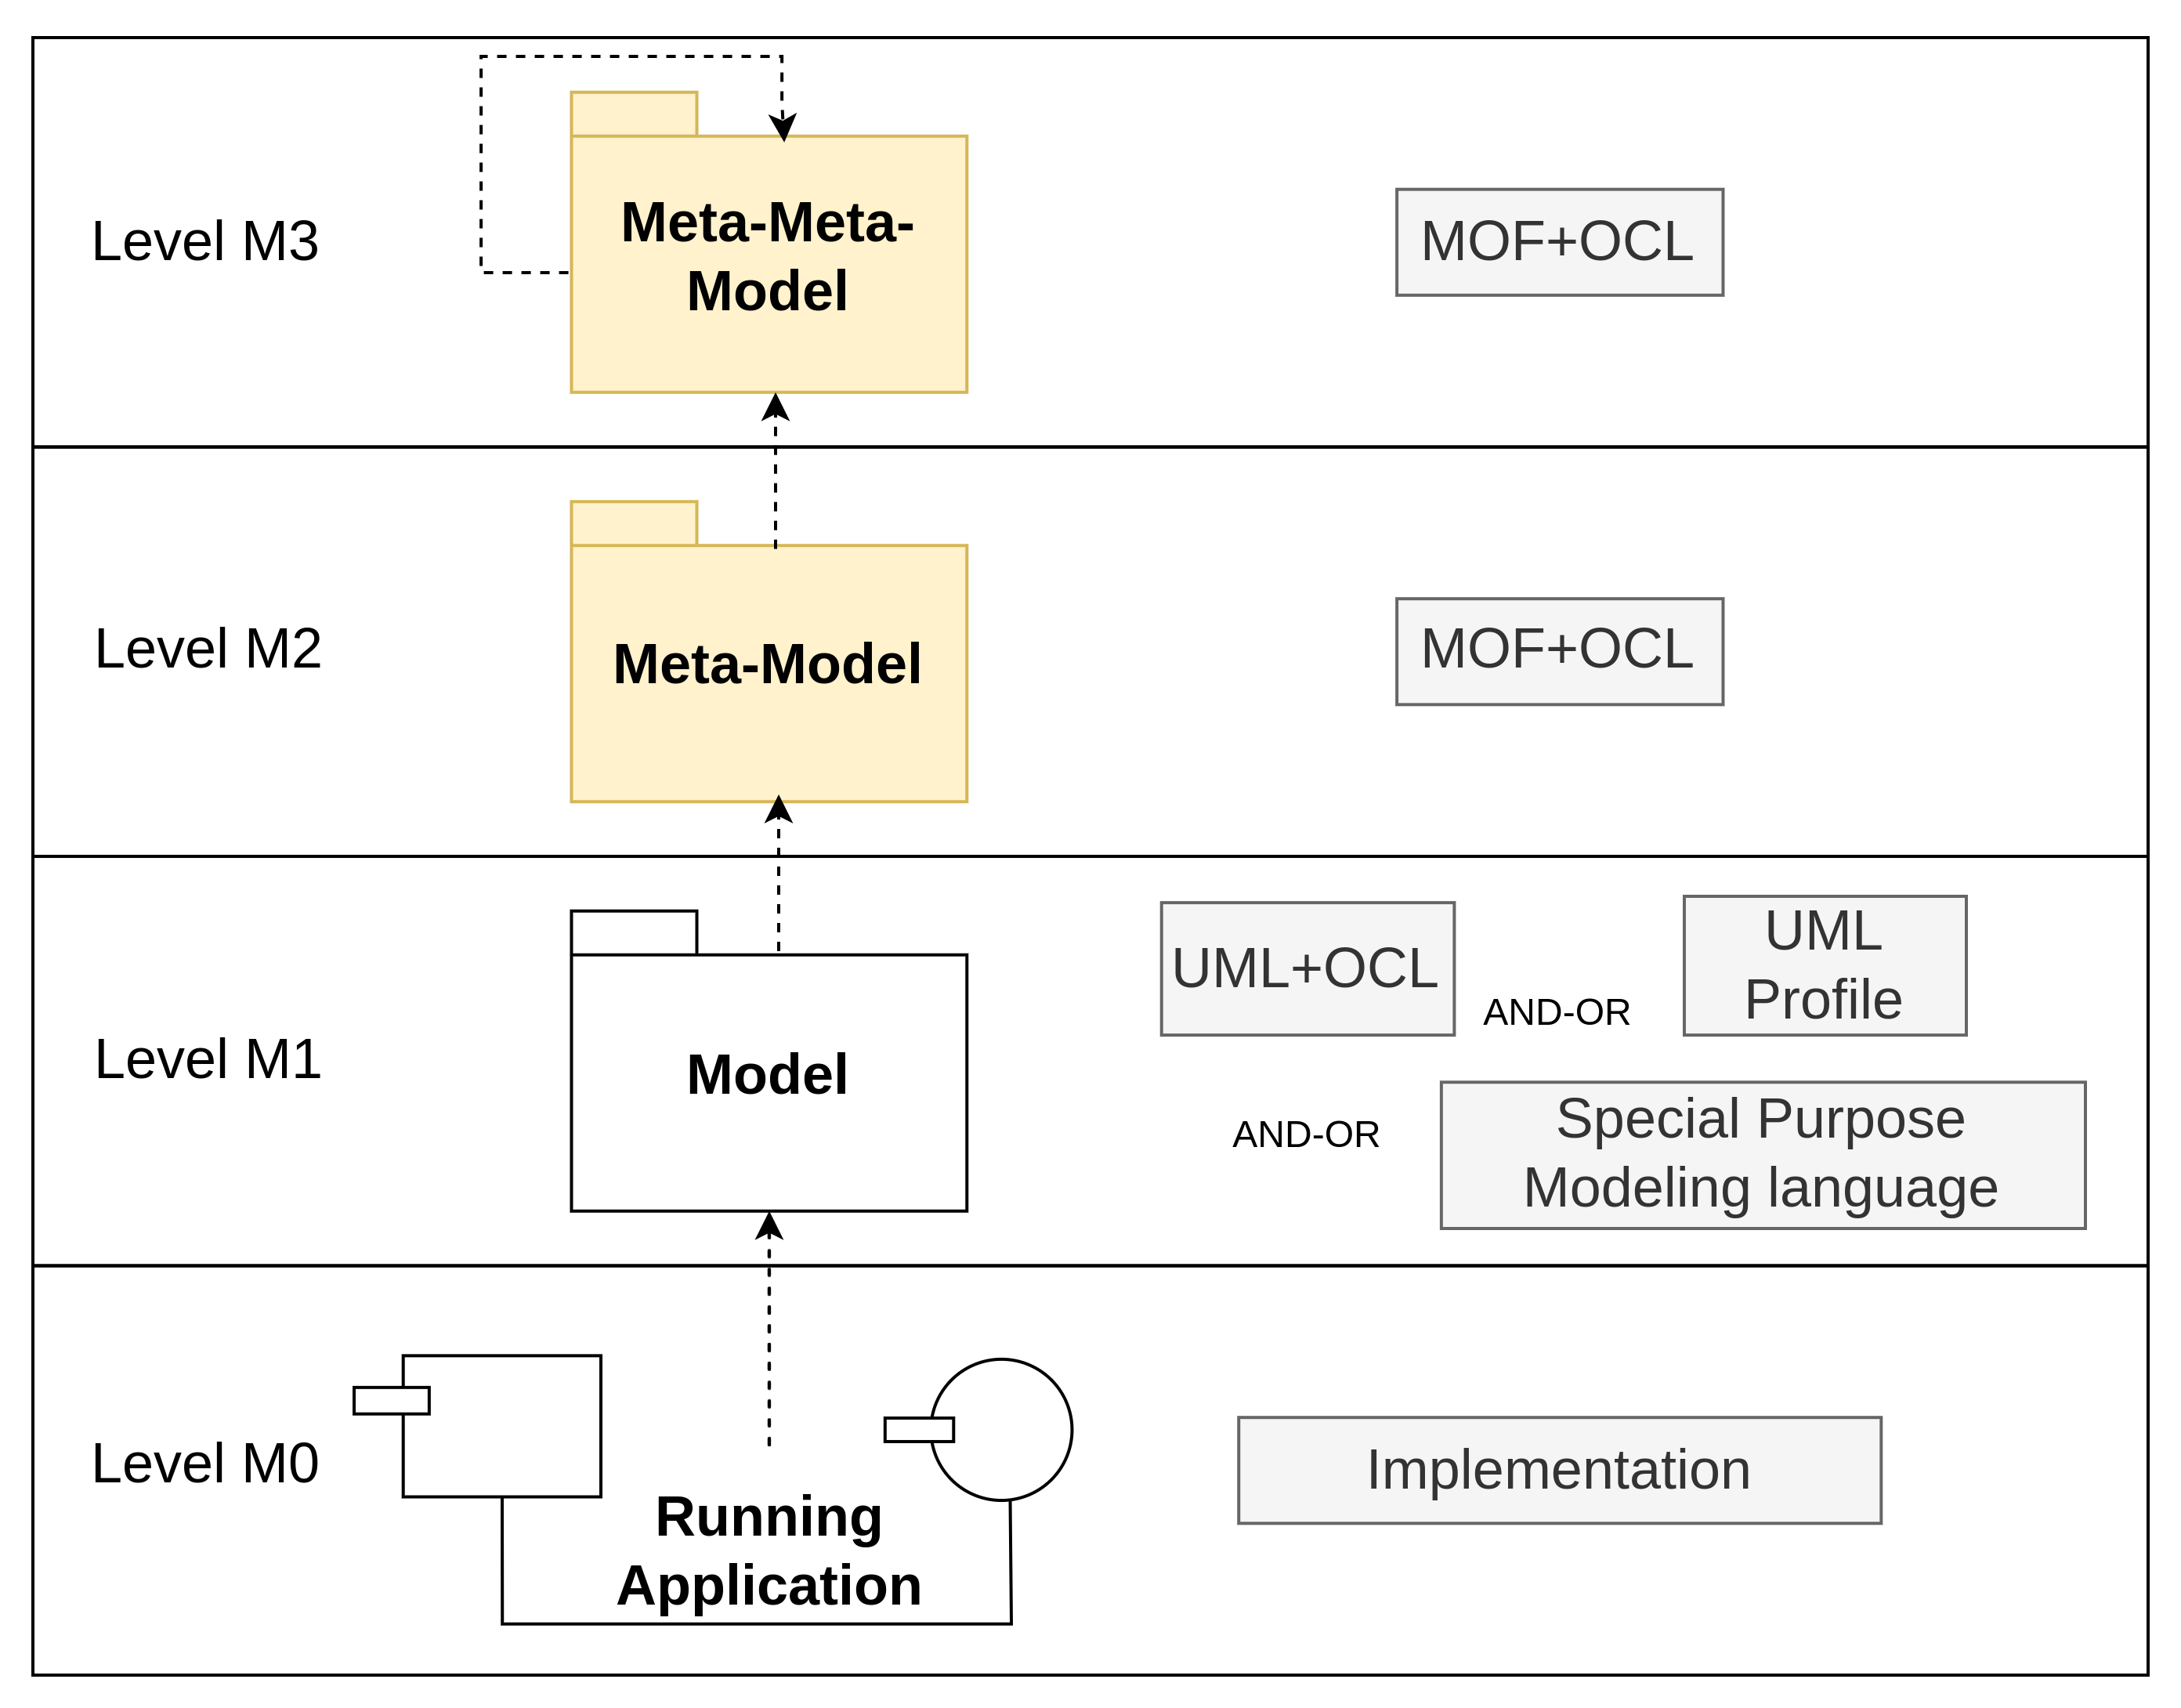
\includegraphics[width=0.6\linewidth]{./pics/soaPics/mofmodellevels2.png}
	\end{center}
	\caption{MDA’s Modeling Level Hierarchy}
	%	{\footnotesize Titre plus long avec des explications.}
	\label{fig:mofmodellevels}
\end{figure}
\begin{figure}[htbp]
	\begin{center}
		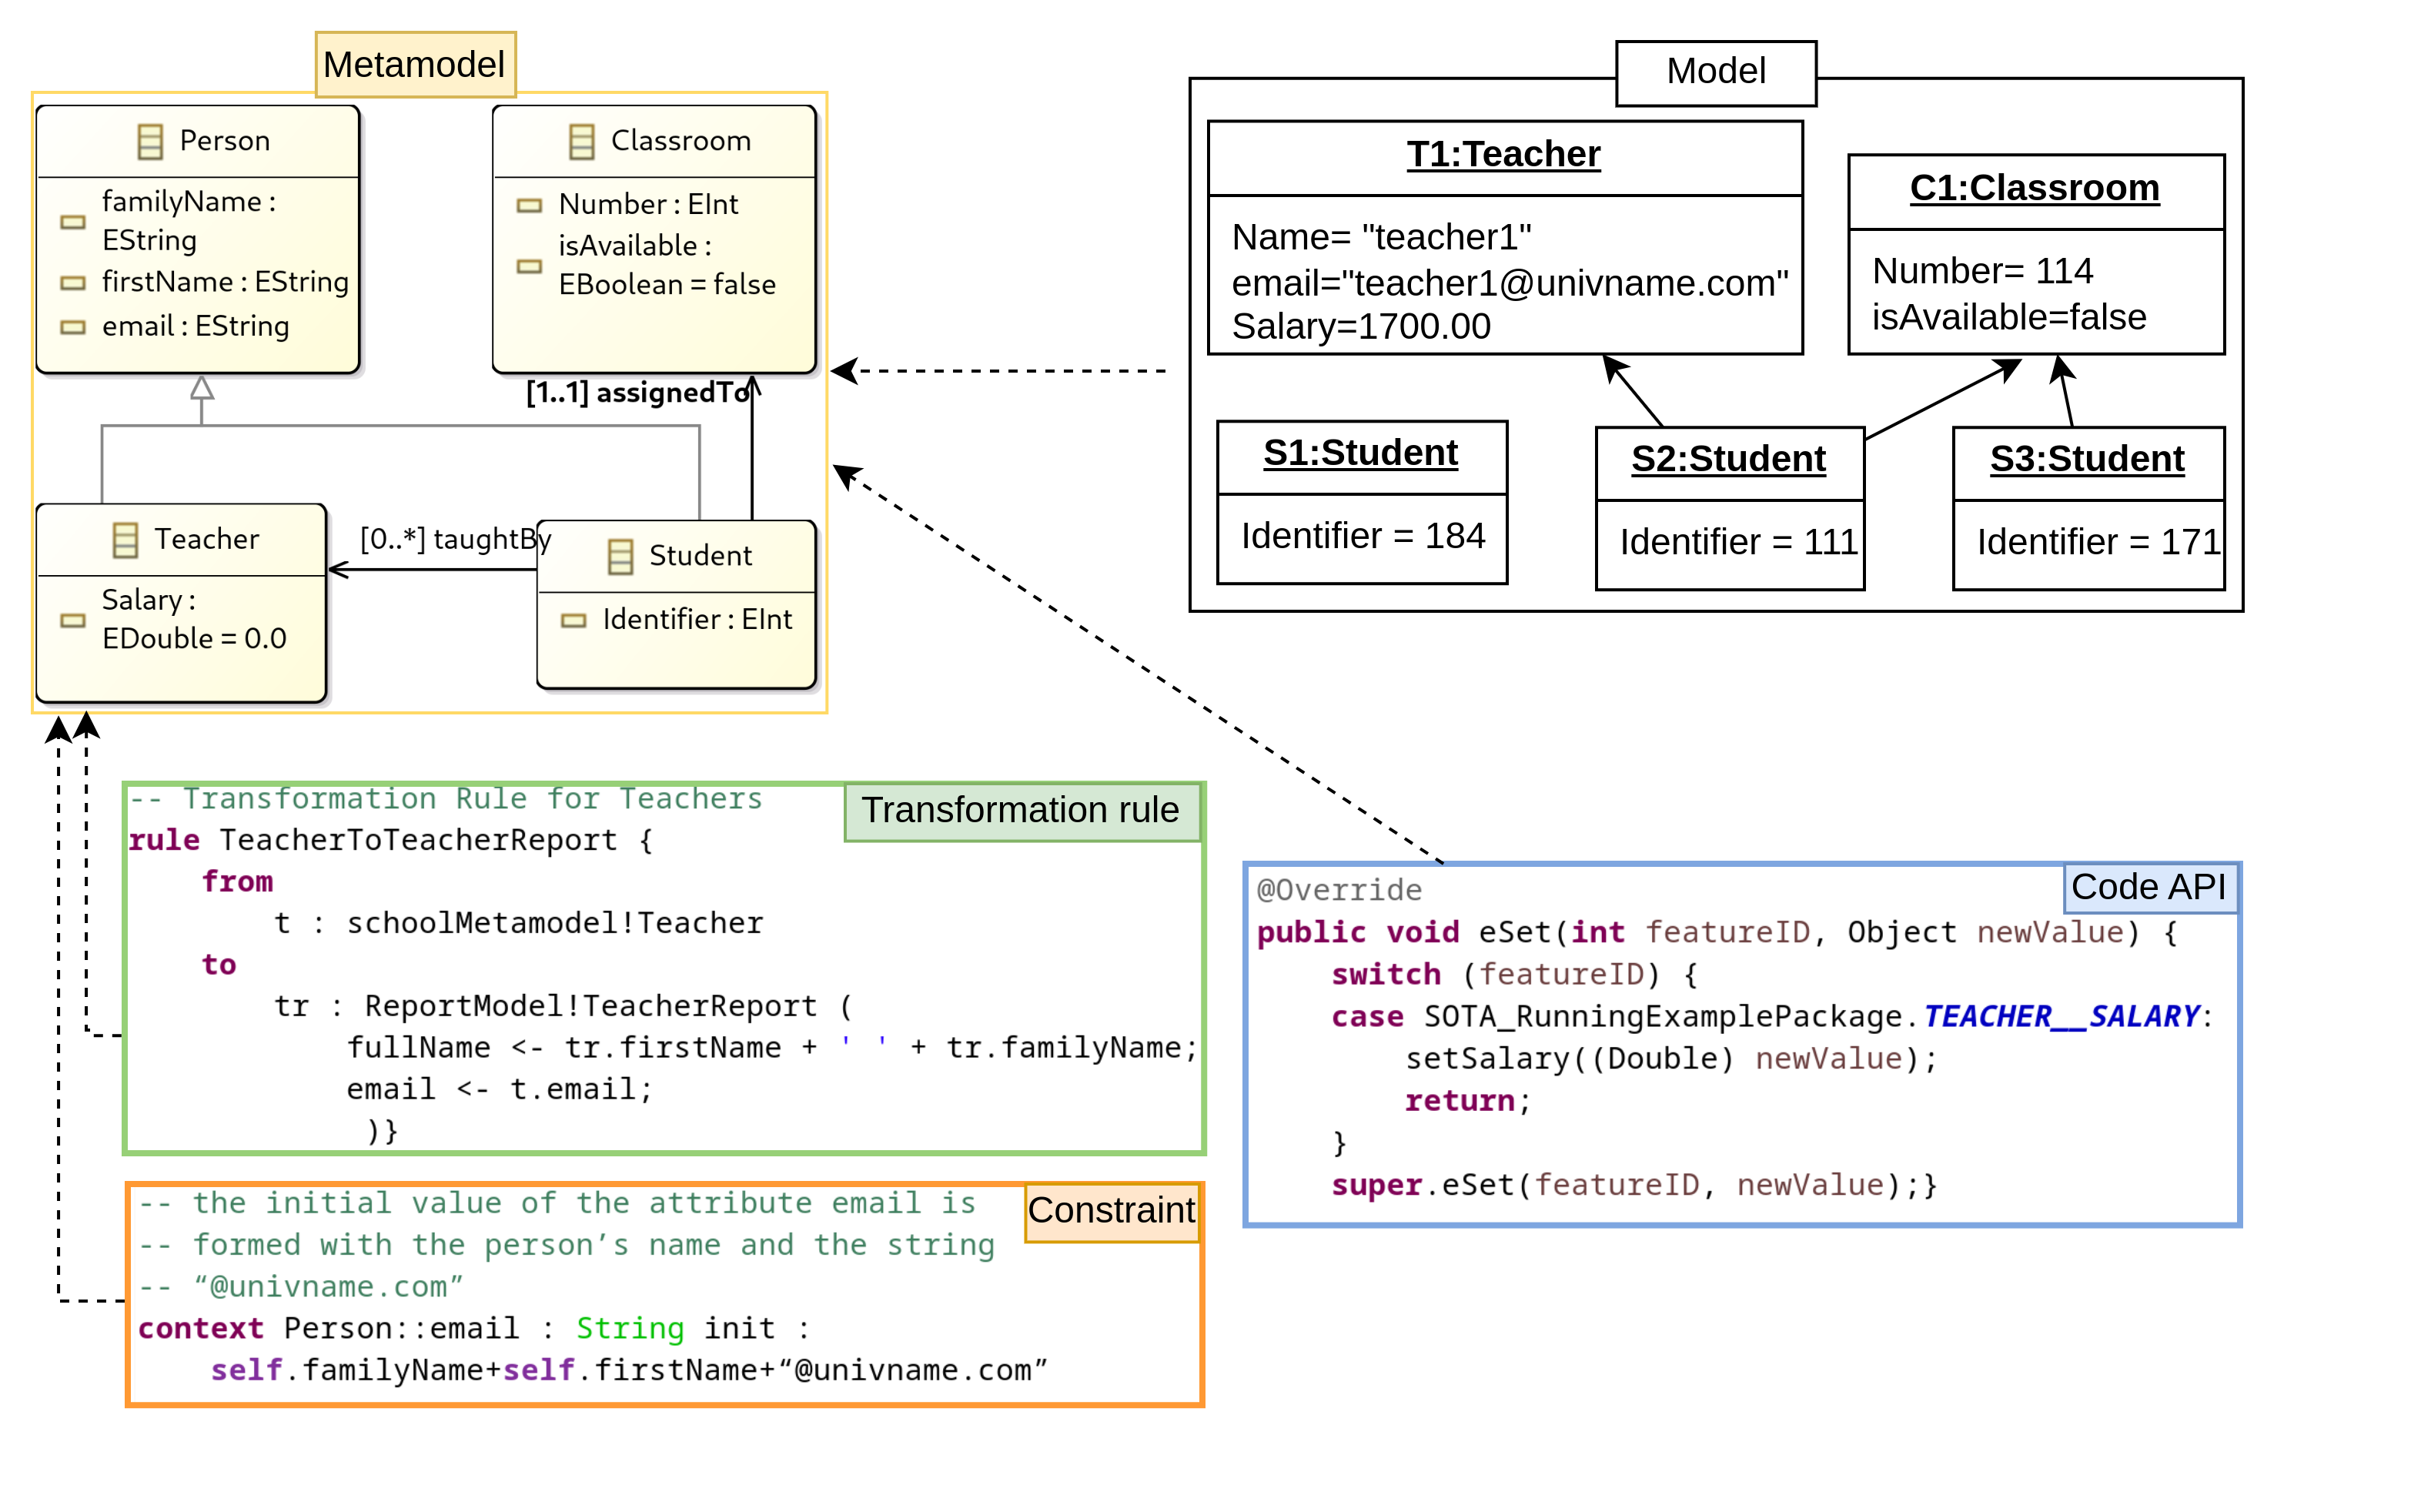
\includegraphics[width=\linewidth]{./pics/soaPics/notabstractecosystem2.png}
	\end{center}
	\caption{MDE Ecosystem}
	%	{\footnotesize Titre plus long avec des explications.}
	\label{fig:mde_ecosystem}
\end{figure}
\begin{itemize}
\item The construction of metamodel itself: it describes the abstract syntax of target software languages or  solution system.
\item Model validation: models are validated against the constraints defined in the metamodel. 
\item Model-to-model transformations: such transformations are defined as mapping rules between source model and a target model .
\item Code generation: it consists of automatically producing source code from models, bridging the gap between high-level abstractions and executable software.
\item Tool integration: based on the metamodel, modeling tools can be adapted to the respective domain. 
\end{itemize}


In the context of Domain-Specific Languages,  represent an essential application of metamodels in practice. A DSL is a specialized language tailored to the needs and constructs of a specific domain, enabling domain experts to express solutions at a higher level of abstraction without delving into general-purpose programming complexities. These languages are typically defined by a metamodel that establishes their syntax and semantics, ensuring consistency and precision. By leveraging metamodeling to create DSLs, engineers can align software artifacts closely with domain-specific requirements, enhancing clarity, maintainability, and automation potential in the software development process \cite{volter2013model}. 

%The metamodel is the basis for the automated, tool-supported processing of models. On the other hand, a suitable concrete syntax is the interface to the modeler and its quality decides what degree of readability the models have \cite{stahl2006model}.

%Metamodeling tools/languages/techniques examples :

%// Add figure?

Metamodeling languages are classified into two categories, namely linguistic and ontological \cite{gavsevic2007metamodeling}. Linguistic metamodeling represents a way for defining modeling languages and their primitives (e.g., Object, Class, MetaClass) on the layer of a metamodel. Ontological metamodeling aims to represent domain knowledge accurately. It is concerned with semantics and meaning, e.g., OWL\footnote{https://www.w3.org/TR/owl-features/}. Linguistic metamodeling aims to define a language for creating models. it is concerned with syntax and structure.
I can use a different classification by purpose: General Purpose Modeling Languages and Domain-Specific Modeling Languages~\cite{de2012domain}. General Purpose Modeling Languages as for example : UML and its variants, generic metamodeling frameworks, such as MOF \footnote{https://www.omg.org/mof/}, and Ecore \footnote{https://eclipse.dev/modeling/emft/search/concepts/subtopic.html}. As examples of DSLs, I cite sysML and EXPRESS DSL~\cite{wortmann2020modeling}.

In MDE, there are language workbenches that are used for language creation, such as Xtext, MetaEdit+ \cite{wortmann2020modeling}.
% Add figure for above languages/techniques/frameworks

%\textbf{Generated artifacts, artifacts linked to the metamodel}


%Metamodel is the backbone in model driven engineering. 
In the language modeling ecosystem, other artifacts are created by the mean of the metamodel. By definition, a model is an instance of a metamodel, which means that the metamodel defines the concepts with which a model can be created. The created models can also be validated through a set of constraints to check the models' correctness. Constraints are written in Object Constraint Language. They precise specifications on the model that cannot be  expressed by diagrammatic notation. In order to save effort and avoid errors, models transformation is one of the common automated tasks in Model-driven engineering. Model transformation are expressed in  Transformation Languages for example, ATL). A transformation consists of a set of rules that map the source metamodel elements to the metamodel target’s elements. All of these artifacts have their specific tools and represent an important topic of research in MDE.

%// Add example of Metamodel+ model+constraint+transformation ?

%ex constraint : the age of a person is not negative, a person is younger than its parents
%Automation in the ecosystem
%code gen 
%tests
\section{Automation in the MDE ecosystem}
\label{mde_automation}
%Brief description about automated tasks in MDE.
 Automation plays a pivotal role within the MDE ecosystem. It is considered as one of the most important advantages of MDE. This section explores the significance of automation in MDE, particularly in the code generation activity and during the evolution of the metamodel cornerstone artifact.
 
 % This section explores also the impact of automation on the development lifecycle.% and key strategies for achieving efficient model-driven processes.

\subsection{Code Generation}

One of the most important activities in MDE is the code generation activity. It is recurrent, and its automation enhances the productivity and the cost. For example, Eclipse Modeling Framework built-in code generator allows to generated a java API from an Ecore metamodel. The generated code API structure and technical choices are done to fit Java programming language and Model-Driven Engineering abstraction standards and principles (e.g., each metaclass is used to generate an interface and concrete implementation class that extends the generated interface, pattern observer).
% to have an efficient as possible
 The annotation \textit{@generated} is used to mark generated interfaces, classes, methods, and fields. This annotation can be used to differentiate the generated code from the manually written one.

In Eclipse Modeling Framework, two model resources (files) are manipulated: the .ecore file that contains  XMI serialization of the Ecore model and the .genmodel for the serialized generator model. The Ecore file is the document that contains the metamodeled main concepts that are used in code generation process.

%\textcolor{blue}{Develop this paragraph?}
\subsection{Software evolution}
From operating systems to mobile apps, software is the cornerstone of modern innovation. However, software does not remain static, it evolves over time to meet new demands, address challenges, and incorporate advancements. Here some numbers showing how much a software can evolve. Let's take Eclipse Modeling Framework (EMF) as a first example from MDE context. EMF\footnote{\url{https://github.com/eclipse-emf/org.eclipse.emf}} has~65 releases, with~10374 commits, and more than~823k lines of code. Another example from MDE is UML \footnote{\url{https://github.com/eclipse-uml2/uml2}} with~2806 commits and more than~716k lines of code. The third example is Linux kernel \footnote{\url{https://github.com/torvalds/linux}} with~1324878 commits and~40 million lines of code. Then
chromium \footnote{\url{https://github.com/chromium/chromium.git}} with~1524157 commits and more than~32 million lines of code. The last example is
cpython \footnote{\url{https://github.com/python/cpython}} with~124936 commits, more than~350k lines of C code and~600k lines of python code.
\begin{figure}[t]
	\begin{center}
		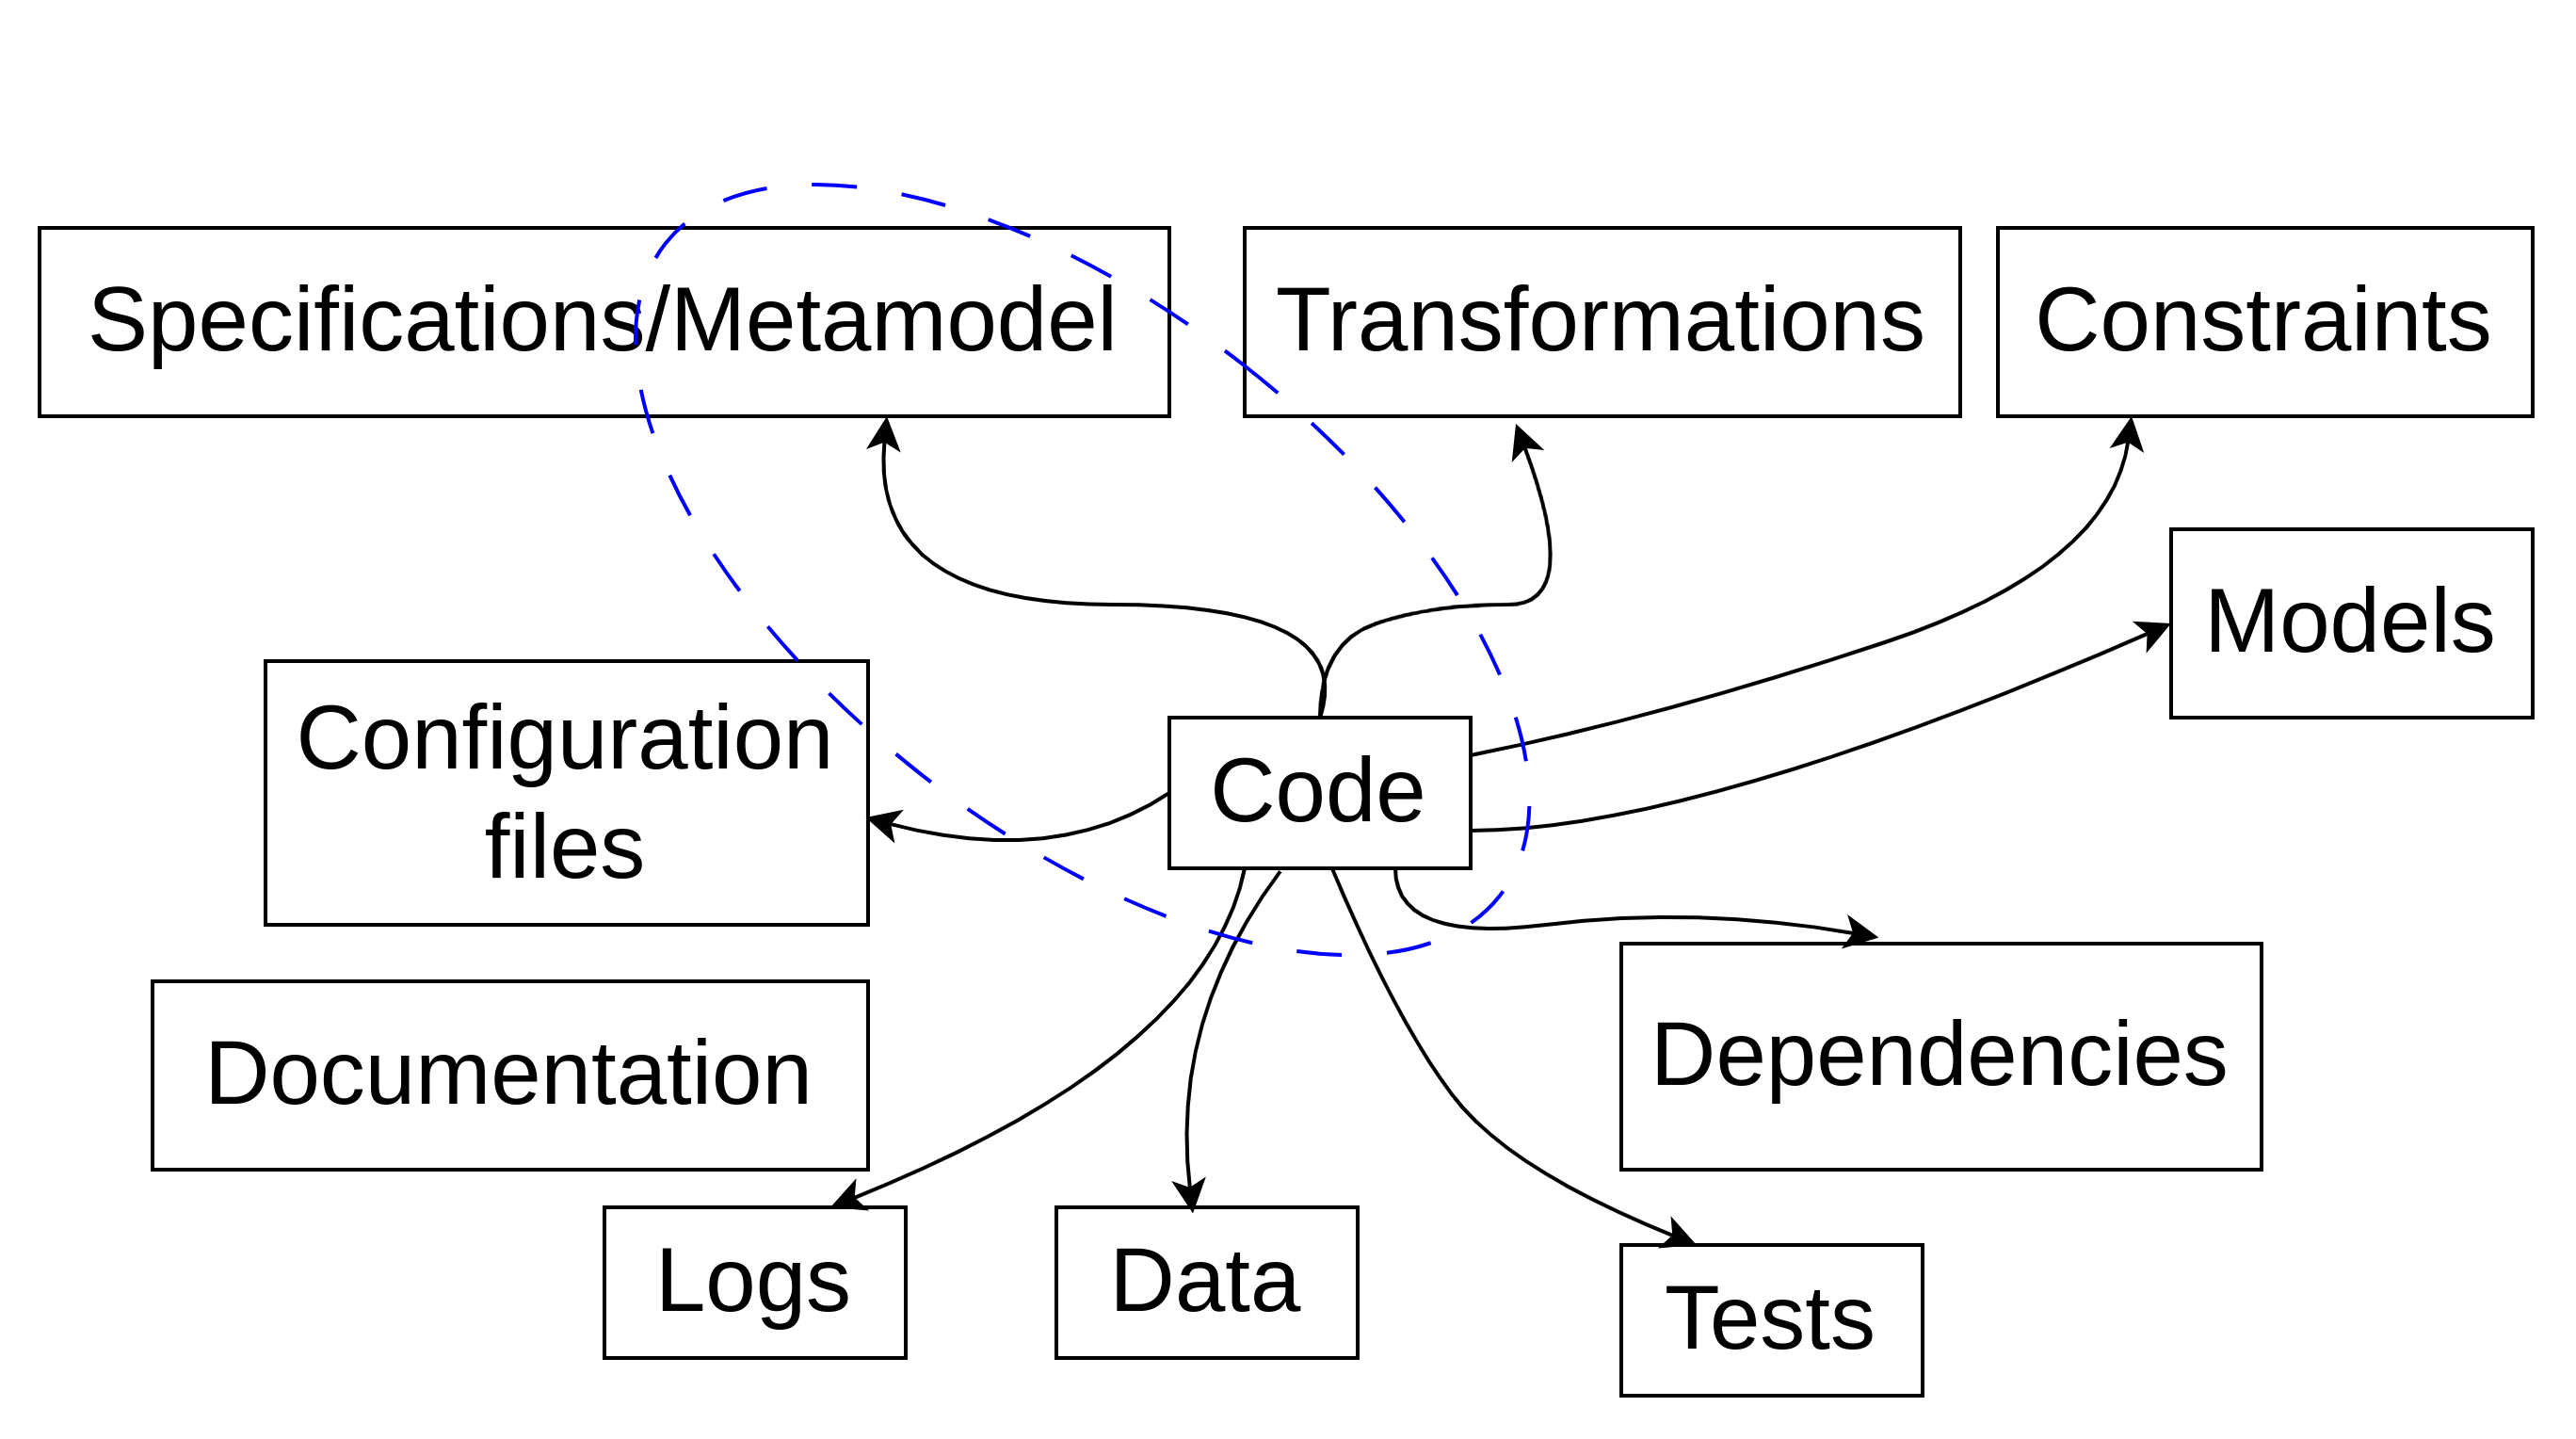
\includegraphics[width=0.6\linewidth]{./pics/soaPics/softwareartifacts.png}
	\end{center}
	\caption{software artifacts}
	\label{fig:softwareartifacts}
\end{figure}
During the software development process, software artifacts are meant to be changed, due to many reasons: client requirements and domain specifications, software maintenance, or bug correction. The evolution can impact one artifact ore more in the software ecosystem (Figure \ref{fig:softwareartifacts}). Like any other software system, modeling languages are the subject of an inevitable evolution, during their process of building, multiple versions are developed, tested, and adapted until a stable version is reached. 

Different types of evolution are categorized depending on the impact and purpose of the applied modifications \cite{lientz1980software,Swanson1976}:
\begin{itemize}
	
	\item  Corrective: aims to correct discovered problems and inconsistencies, such as processing failures, performance failures, or implementation failures by applying a set of reactive modifications of a software product.  
	
	\item  Adaptive: in case of changing environment, such as changes in data environment or processing environment, this evolution aims to keep a software product usable.
	
	\item Perfective: this evolution aims to improve functionalities, to enhance the performance, reliability, or to increase the maintainability of a software.  
	
\end{itemize}
%It is unavoidable to change, whether to answer to requirement modifications and/or technological progress.
The term \textit{Evolution} can be refined as the literature presents various related terms like: Maintenance, Refactoring, and \textbf{Co-evolution}, which are different types of modifications that could be applied on a software. There is no clear definition for each of them, however, in figure \ref{fig:evolutiontypes} I describe the relationship between these terms by intent and by artifacts on which the task is applied.

%/Why we need to perform evolution ?
%examples?
%TODO Add defs references

\textbf{Evolution}: any adaptation that occurs in the software in response to new requirements. These requirements are the consequence of the past experience of the users that feeds the developers' learning. \cite{bennett2000software}. 

\textbf{Maintenance}: It is modifying a software product after delivery to correct faults, to improve performance, or to adapt the product to a changing environment \cite{schneidewind1987state}.

\textbf{Refactoring}: It is an oriented object term, that means behavior-preserving modifications of software, to make it easier to understand and to change or to make it less susceptible to errors when future changes are introduced \cite{mens2004survey}. 

\textbf{Co-evolution}: It consists of the process of adapting and correcting a set of artifacts $A_1$, $A_2$, ...$A_N$ in response to the evolution of an artifact B on which $A_1$, $A_2$, ...$A_N$  strongly depend, for example the co-evolution of models with the evolving metamodel as used in Kessentini et al. paper \cite{Kessentini2016automated}, and the co-evolution of API/client as used in Eilertsen et al. paper \cite{8443581}. The term "Coupled evolution" was also mentionned in the work of Herrmannsdoerfer et al. in the context of metamodel and model co-evolution \cite{herrmannsdoerfer2009cope}

%\begin{figure}[htbp]
%	\begin{center}
%		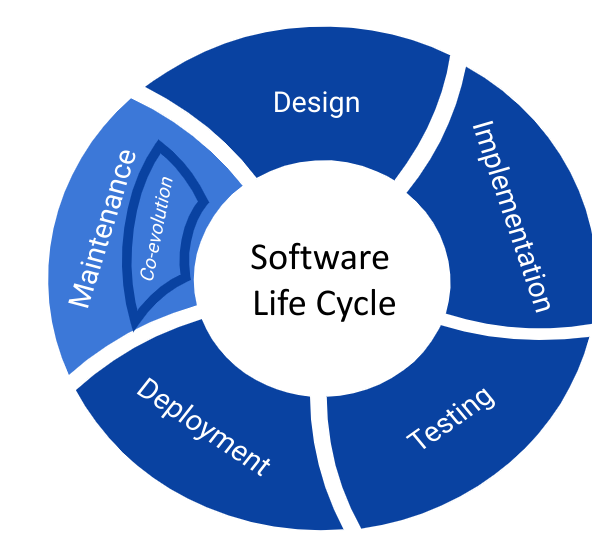
\includegraphics[width=0.6\linewidth]{./pics/soaPics/solicy.png}
%	\end{center}
%	\caption{Software Life Cycle ( not sure to include)}
%	{\footnotesize Titre plus long avec des explications.}
%	\label{fig:softwarelifecyle}
%\end{figure}



\begin{figure}[t]
	\begin{center}
		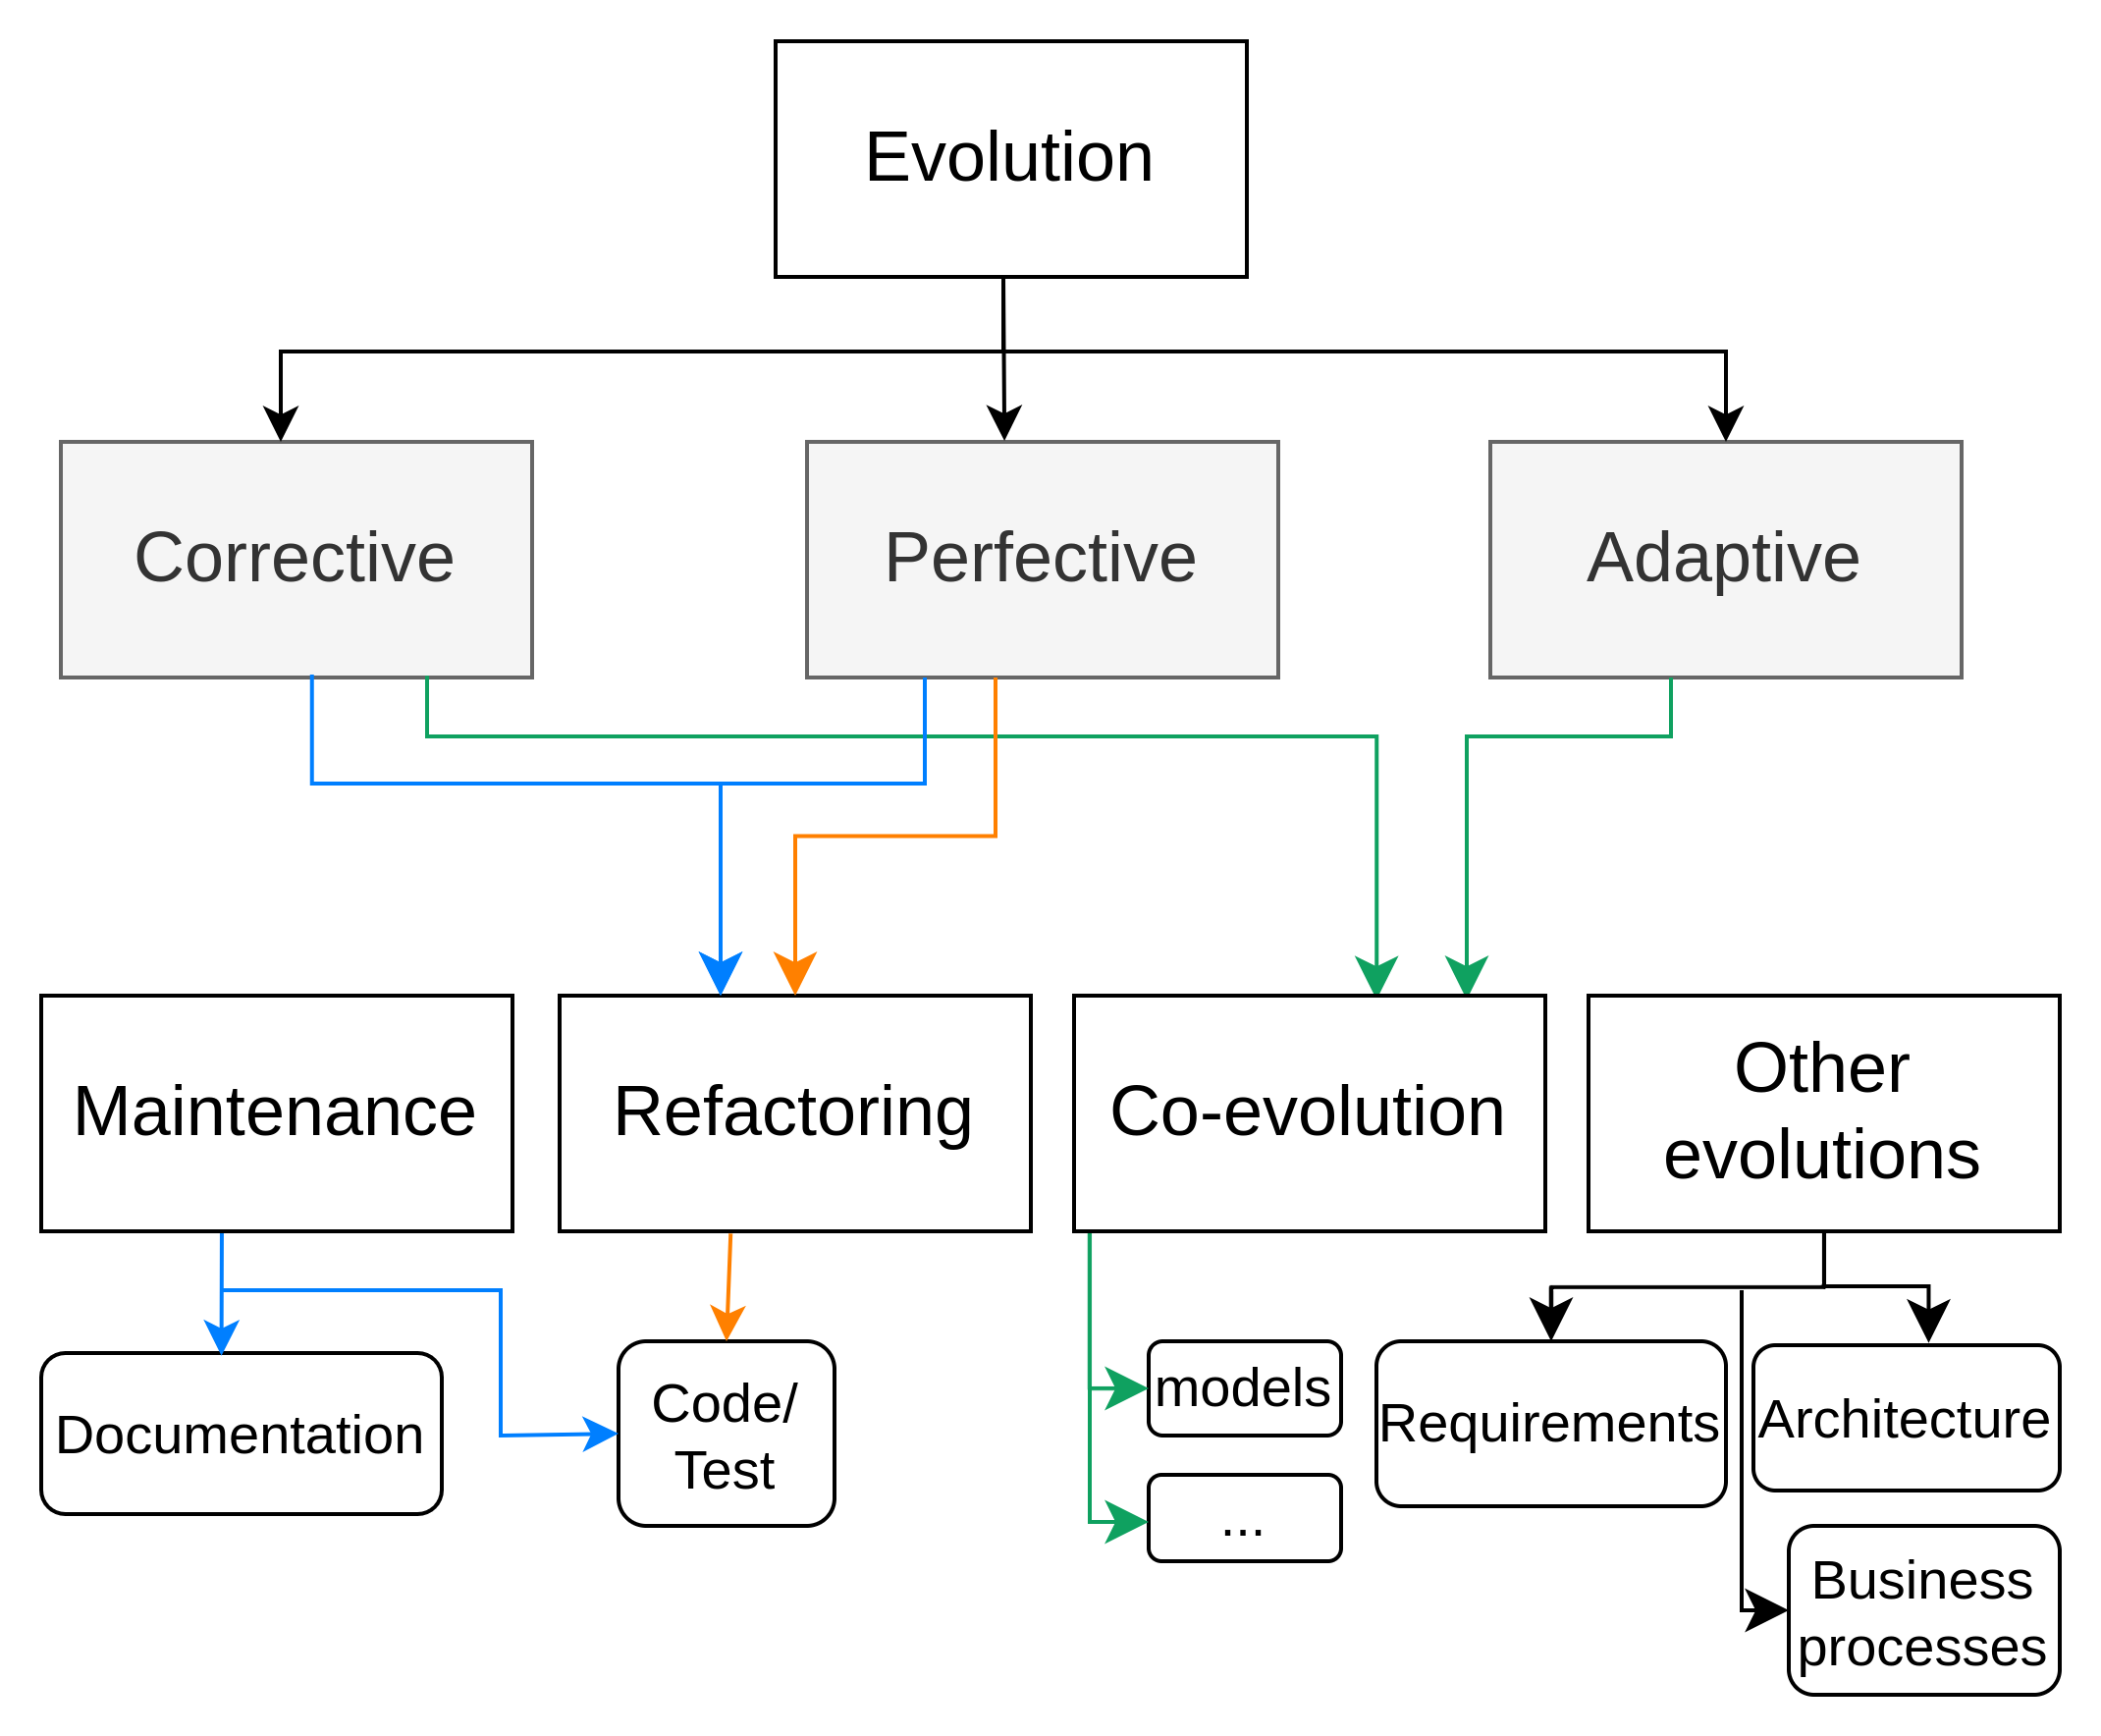
\includegraphics[width=0.6\linewidth]{./pics/soaPics/evolutiontypes.png}
	\end{center}
	\caption{Evolution related terminology}
	%	{\footnotesize Titre plus long avec des explications.}
	\label{fig:evolutiontypes}
\end{figure}

\section{Large Language Models}
\label{llm}
In this section, I outline the fundamental concepts related to Large Language Models, namely Transformer models and prompt engineering. I give a short historical view to understand the added value of using LLMs in my third contribution (cf. Chapter \ref{chapitre3}).

\subsection{From Transformer Models to Large Language Models}

%Rule-based and hand-crafted solutions are rigid and hard to scale.
Machine learning field introduced statistical models that learn from input data. As an improvement of traditional machine learning approaches, neural networks brought breakthroughs in image and speech recognition, inspiring their application to Natural Language Processing (NLP). A markup point in the history of machine learning is The Attention Mechanism \cite{10.5555/3295222.3295349}. It allows models to focus on relevant parts of input sequences, significantly enhancing translation and comprehension tasks.
This mechanism allows the model to weigh the importance of all words in a sequence simultaneously, leading to: 1) Parallel processing for a faster computation, and 2) Better handling of long-range dependencies. After neural networks and Attention mechanism application in NLP, the transformer models appearance first in 2018, marked by the emergence of BERT and its variations \cite{DBLP:journals/corr/abs-2302-09419}.


%Bert def and caract vs traditional models)
\textbf{BERT} (Bidirectional Encoder Representations from Transformers) is an encoder-only transformer model owned by Google \cite{devlin2019bertpretrainingdeepbidirectional}. Regarding data corpus, BERT is pre-trained from  Wikipedia and Google’s BooksCorpus. Another remarkable model is \textbf{BART} (Bidirectional and Auto-Regressive Transformers). It was introduced by Lewis et al. \cite{lewis2019bartdenoisingsequencetosequencepretraining}.
Unlike BERT’s encoder-only design, BART’s architecture is a sequence-to-sequence model, featuring both encoder and decoder components.
In 2018, OpenAPI has launched another large scale pre-trained transformer model: GPT, then \textbf{GPT-3} in 2020 \cite{10113601}.


 

%BERT, BART, and GPT 
%main doc :Utilizing Large Language Models for Question Answering in Task-Oriented Dialogues)

Note that in the field of LLM, new approaches are being developed at a rapid pace. Thus, rather then latest models, I selected models that have marked a turning point in the history of LLMs: BERT, BART, and GPT to include in this short LLM background. No global and detailed comparison between GPT, BERT, and BART is established. However, some works have conducted targeted comparisons in specific context. For example, Yokoyama et al. compare between Chatgpt and BERT in security bug identification topic \cite{10685583}. Table \ref{table:bertvsbartvsgpt3} summarizes the key differences between BERT, BART, and GPT-3 depending on: their architecture, learning data, number of parameters, performance speed, application domain in which the model is most efficient, and the respective organizations that created them~\cite{DBLP:journals/corr/abs-2302-09419,lewis2019bartdenoisingsequencetosequencepretraining}.
%https://scholar.google.fr/scholar?as_q=comparison+BERT+chatgpt&as_epq=&as_oq=&as_eq=&as_occt=title&as_sauthors=&as_publication=&as_ylo=&as_yhi=&hl=fr&as_sdt=0%2C5



%Add the comparative table with BART column : https://updf.com/fr/chatgpt/bert-vs-gpt/
\begin{table}[h]
	\vspace{-1.2cm}
	\caption{Comparison BERT, BART, and GPT-3} 
	\label{table:bertvsbartvsgpt3}
\hspace{-2cm}
\begin{tabular}{ | m{2.5cm}| m{4cm}| m{4.5cm} |m{5.5cm} |  } 

	\hline
	\textbf{Functionality}& \textbf{BERT} & \textbf{BART} &\textbf{GPT-3} \\ 
	\hline\hline
	\textbf{Architecture} & Bidirectional encoder-only model that considers both left and right contexts when making predictions. &  Encoder-decoder model, Bidirectional encoder with left-to-right autoregressive decoder it considers both left and right contexts when making predictions. &The autoregressive model generates text by predicting the next word in a sequence based on the preceding words \\ 
	\hline
		\textbf{Data} & Learning on data from sources such as English Wikipedia and BookCorpus 11038 books). & Learning from a combination of books and Wikipedia data &  extremely large corpus of English text data extracted from millions of web pages and then fine-tuned using Reinforcement Learning from Human Feedback (RLHF) \\ 
	\hline
		\textbf{Number of parameters }& $BERT_{base}$ 110 m parameters  $BERT_{large}$ 340 million parameters, a relatively smaller number than GPT-3. & $BART_{base}$ contains 139 million parameters and $BART_{large}$ contains around 400 million parameters&175 billion parameters, far more than any other language model.\\
		\hline
			\textbf{Performance speed?}& faster than BART and GPT-3
			.& Decoding step and the number of parameters make it slower than BERT& the slowest one, because of the number of parameters, size of data, and the complex architecture.\\
		\hline
			\textbf{Application (domain)}&Top performance on a range of tasks, including text classification.
			Requires further fine-tuning and learning to adapt to new domains and tasks.&particularly effective when fine-tuned for downstream NLP tasks, especially text generation&It has shown remarkable performance on a wide range of natural language processing tasks.
			Can be generalized to new domains thanks to learning in a few steps, and adapted to new tasks thanks to transfer learning.\\
			\hline

\textbf{Origin organisation}&Google AI&Facebook AI& OpenAI\\
\hline		
\end{tabular}
	\end{table}
%Large scale pre-training, high scalability.


\subsection{Prompt Engineering}


\textbf{Definition -- Prompt Engineering.} It consists of techniques that are used to converse with LLMs. As a subdomain of LLMs field, it represents an active and rapidly evolving area of study. Frieder et al. confirm the impact of having a correct prompt structure in the capability of LLMs' problems resolution \cite{10.5555/3666122.3667327}. 
Although GPT-3 may have popularized these prompt engineering techniques \cite{10.5555/3495724.3495883}, other LLMs are capable of these generalization techniques, such as PaLM \cite{10.5555/3648699.3648939} and Chinchilla \cite{10.5555/3600270.3602446}.

Here I define two popular categories of prompt-engineering techniques: zero-shot/few-shot prompting and Chain-of-Thought reasoning:
\begin{itemize}
	\item Few-shot/zero-shot prompting: In few-shot prompting, the prompt is enriched with one or more examples of the task in the prefix before being asked to perform the task on new data. These examples serve as a way to prime the model to produce the desired output. In zero-shot prompting, no example is provided \cite{brown2020languagemodelsfewshotlearners,10.1145/3560815}.
	
%	Whatpu example nop , to demo next
	
	\item Chain-of-Thought reasoning: enables complex reasoning capabilities through intermediate reasoning steps. it can be combined with few-shot prompting to get better results on more complex tasks that require reasoning before responding \cite{10.5555/3600270.3602070}.
	
	Note that other techniques can be found in Liu et al. systematic survey of prompting methods in \cite{10.1145/3560815}, and in this prompting guide website \footnote{\url{https://www.promptingguide.ai/techniques}}.
	
	Let's take an example for the prompt "If Alice has 5 apples and gives 3 to Bob, how many apples does Alice have left?". Figure \ref{fig:fewshotexample} shows the prompt content in the case of few-shot prompting, and Figure \ref{fig:cotexample} shows the chain-of thought reasoning for the same prompt.
	
	
	\begin{figure*}[t!]
		\centering
		\begin{subfigure}[t]{0.5\linewidth}
			%\centering
			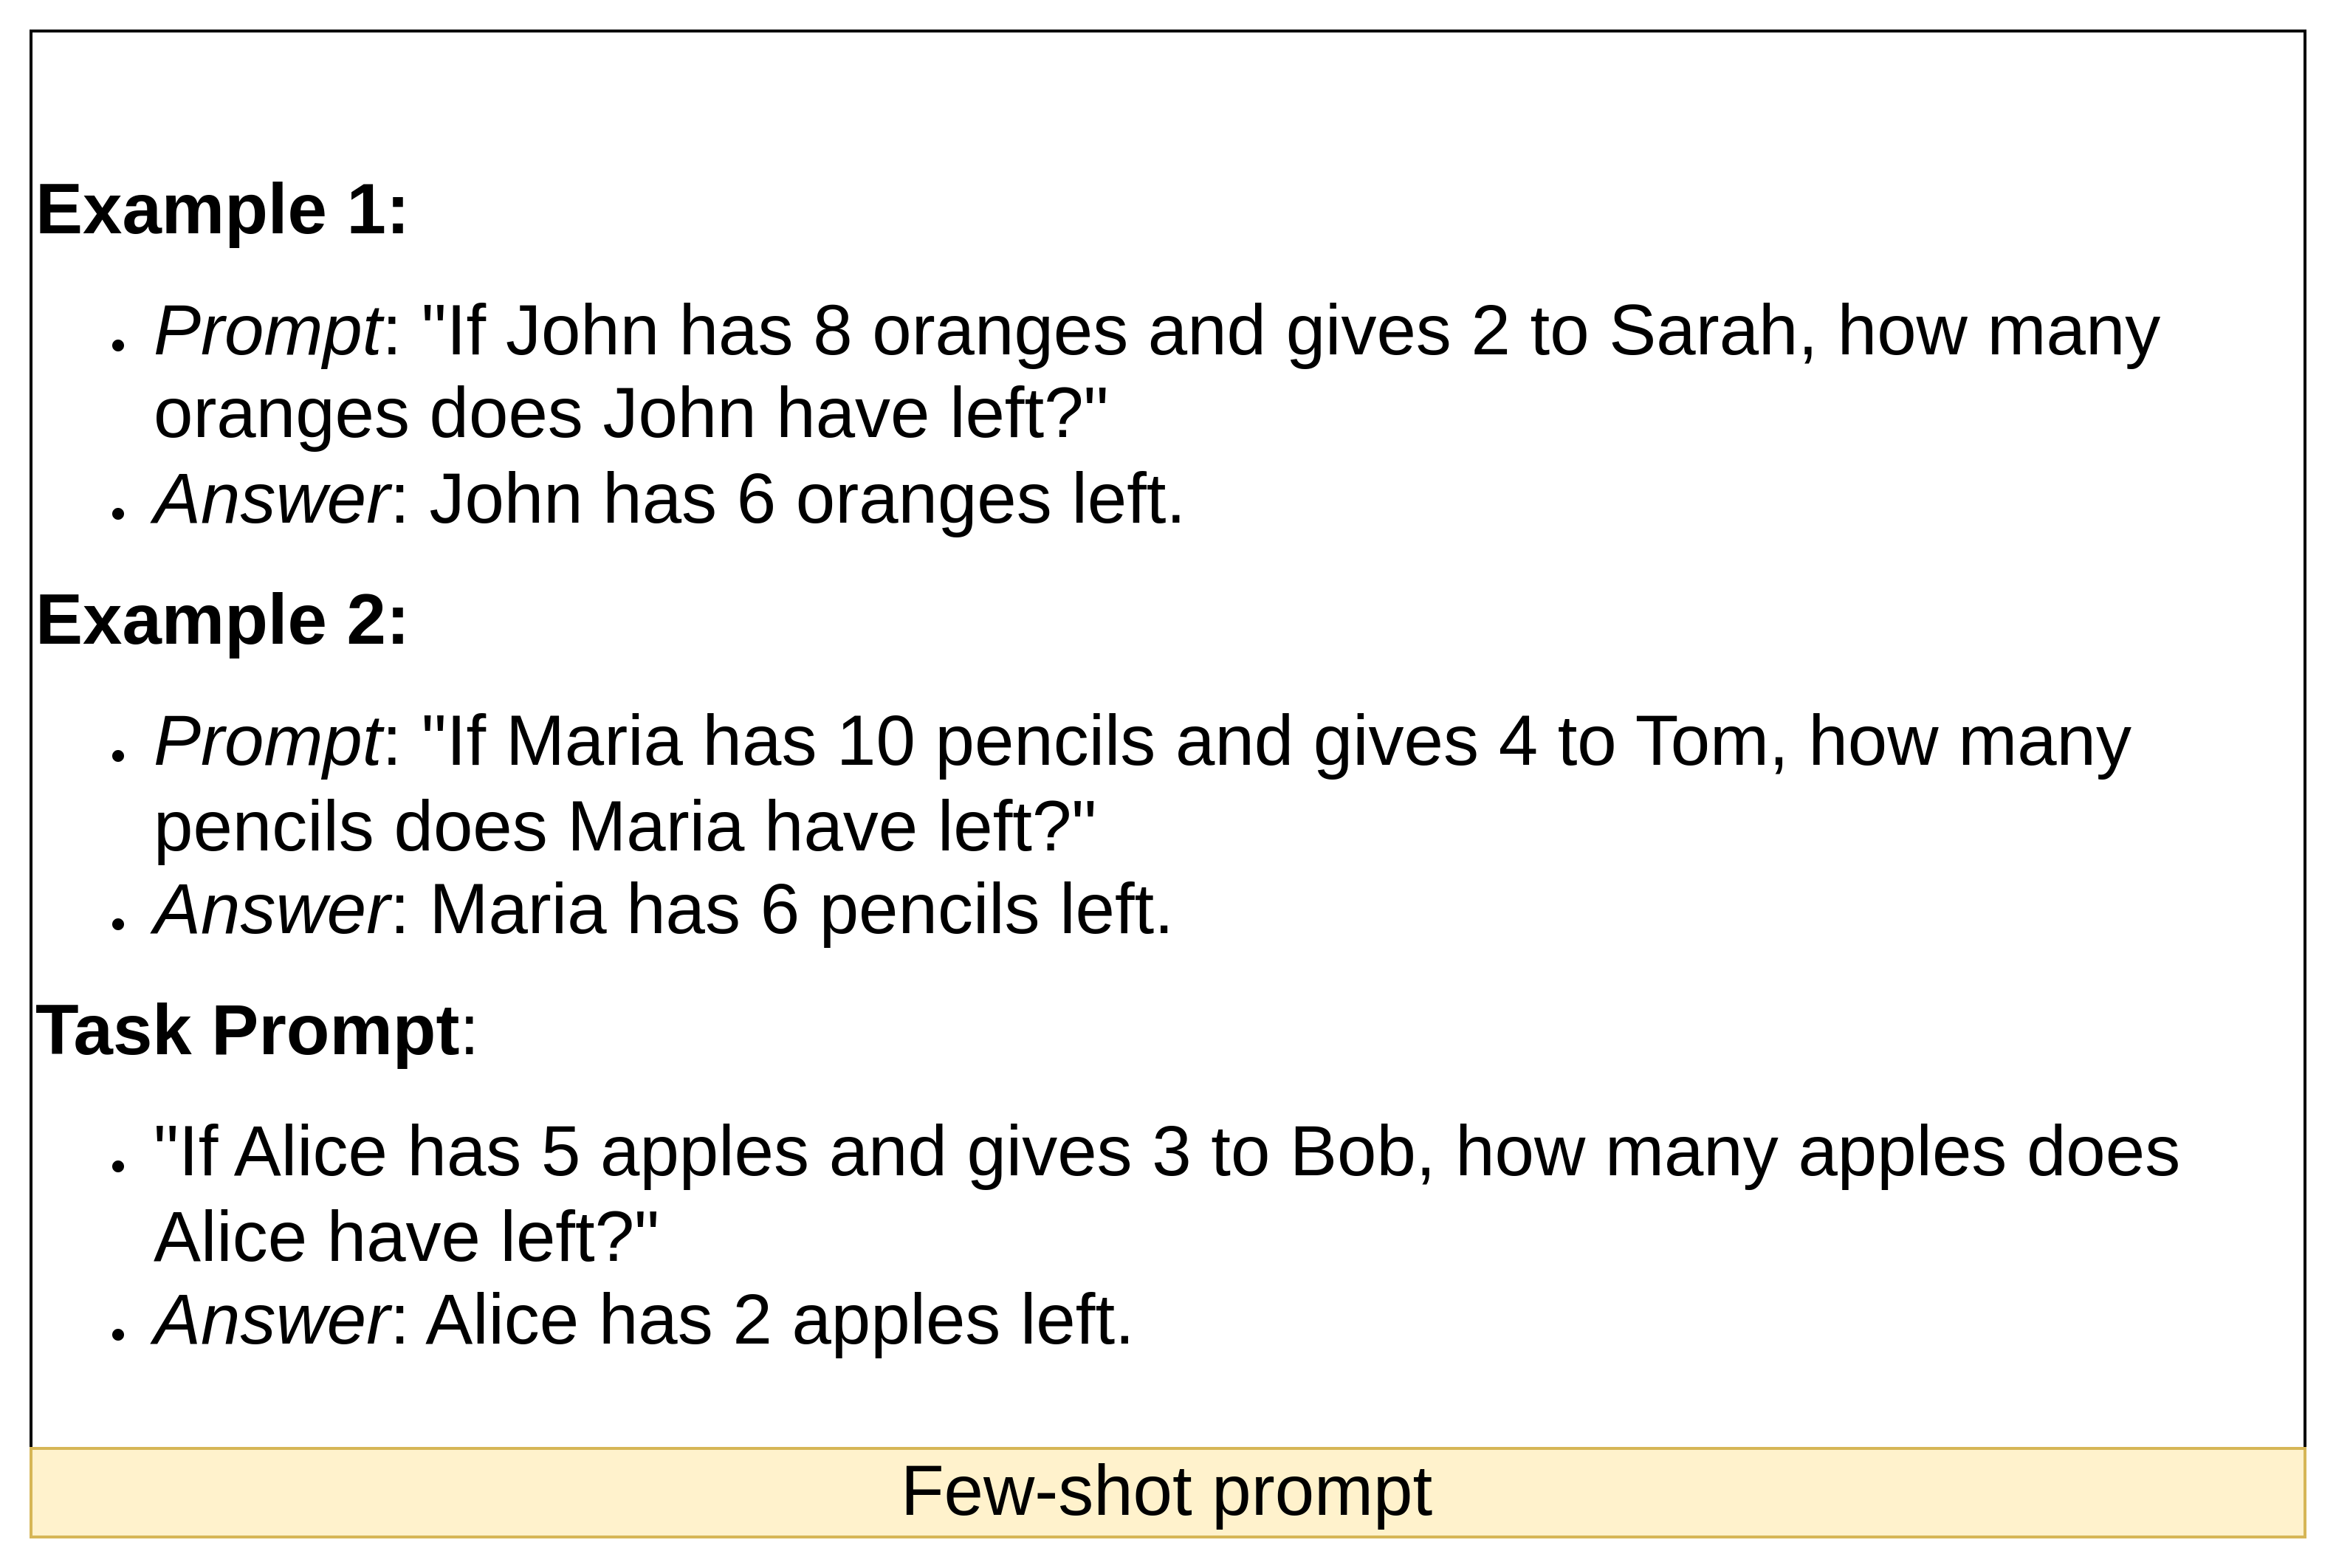
\includegraphics[height=2in]{./pics/soaPics/fewshotpromtexample.png}
			\caption{Few-shot prompt example}
			\label{fig:fewshotexample}
		\end{subfigure}%
		~ 
		\begin{subfigure}[t]{0.5\linewidth}
			%\centering
			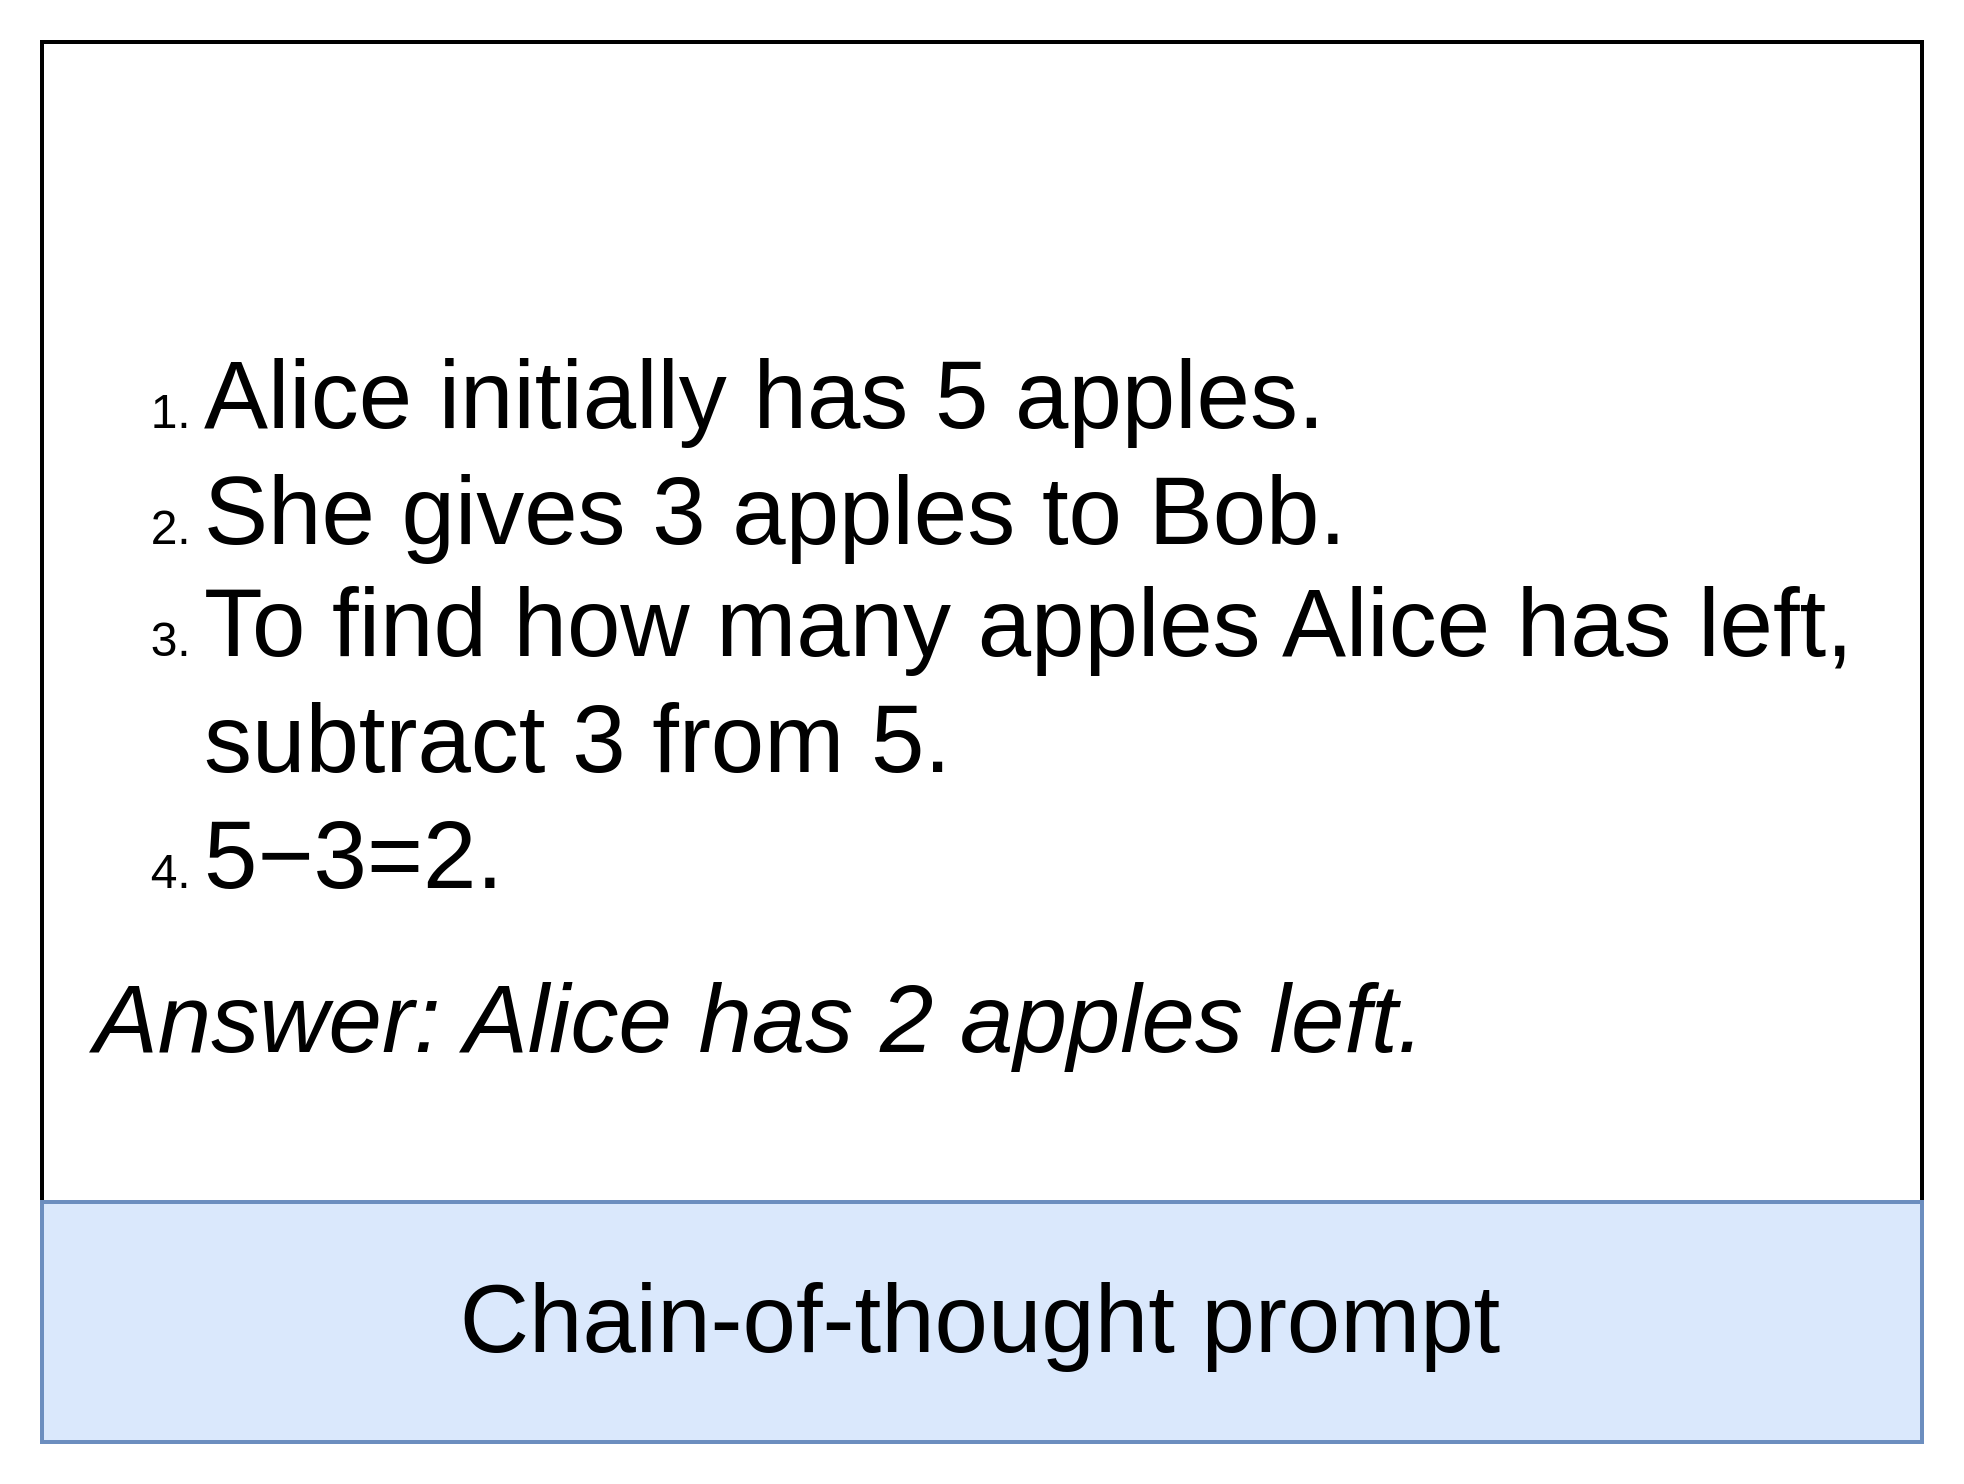
\includegraphics[height=2in]{ ./pics/soaPics/cotpromptexample.png }
		
			\caption{Chain-of-thought prompt example}
			\label{fig:cotexample}
		\end{subfigure}
	%	\label{fig:fewshotcotexample}
		\caption{ Few-shot vs Chain-of thought example }
	\end{figure*}
	
	
	
\end{itemize}
\section{Conclusion}
In this chapter, I provided the essential background for Model-Driven Engineering, covering key aspects such as metamodeling and its related artifacts, automation tasks, and the concept of co-evolution with the different concepts related to evolution. Additionally, an overview of Large Language Models was presented to highlight their relevance in this thesis. This foundation establishes the necessary understanding for the exploration of following chapters.

%definition
\chapter{State Of The Art}
\label{sota}
\chaptermark{State Of The Art}
%offline and online process
In this chapter, I present an overview of what has been done in the field of Model-Driven Engineering in the context of code co-evolution. I split this overview into five  parts. In section~\ref{changedetection}, I present the metamodel change detection approaches. Section~\ref{coevolutionartifacts} presents the co-evolution of model, transformations, constraints with evolving metamodel. In section~\ref{coevolutioncode}, I discuss code co-evolution and relevant literature about API-client evolution, and language evolution. In Section~\ref{behavioralcorrectness}, I browse related work to checking the behavioral correctness of code co-evolution. Section~\ref{llmsforcoevolution}, presents an overview of the use of LLMs in related MDE and SLE tasks. I finish this chapter with a discussion focused on limitations and research gap in Section~\ref{sotadiscuss}.
 \section{Metamodel change detection}
 \label{changedetection}
 One of the intrinsic properties of software artifacts is its continuous evolution~\cite{mens2008introduction}. Like any software artifact, metamodels are meant to evolve to meet the represented domain. %one key sentence of the context
 In this thesis, the context is triggered by the metamodel evolution, that's why I find essential to understand this evolution in detail.
 %metamodel diffing
 A lot of work has been done on metamodel diffing.
 Detection approaches can be classified into two main categories: online\footnote{Offline approaches perform detection after the metamodel has been evolved.} detection approaches, and offline\footnote{Online approaches perform instant detection for each change during the metamodel evolution} detection approaches. This classification can be refined using some factors as detailed by Hebig et al.~\cite{hebig2016approaches}: automation degree, types of detected changes, considered issues (overlap, indefinite length, hidden changes, order of changes, and undo operations)~\cite{hebig2016approaches}.
 	
 \begin{table}[p]
 	\centering
 	
 	\resizebox{16cm}{!} {
 		{\small
 			\begin{tabular}{l|c|c}%|l|l|l|l|l|l|l|}
 			%\hline
 			\toprule 
 			Type & group  & Change name  \\ \midrule
 			
 			\multicolumn{1}{l|}{ Atomic changes}
 			& \multirow{2}{*}{ \begin{tabular}[c]{@{}l@{}} Structural \\ Primitives\end{tabular} } 
 			&  \begin{tabular}[c]{@{}l@{}} Create Package, Delete Package, Create Class,\\Delete Class, Create Attribute, Create Reference,\\ Delete Feature,change type, Create Opposite Ref.,\\Delete Opposite Ref., Create Data Type, \\Delete Data Type, Create Enum, Delete Enum, \\Create Literal,Merge Literal  \end{tabular}
 			\\  \cmidrule{2-3} 
 			& \multirow{2}{*}{ \begin{tabular}[c]{@{}l@{}} Non Structural \\ primitives\end{tabular}} 
 			&  \begin{tabular}[c]{@{}l@{}} Rename, Change Package,Make Class\\ Abstract, Drop Class Abstract,\\ Add Super Type, Remove \\Super Type, Make Attr. Identifier,\\ Drop Attr. Identifier, Make Ref. Composite, \\Switch Ref. Composite, Make Ref. Opposite,\\ Drop Ref. Opposite  \end{tabular}
 			\\   \cmidrule{1-3} 
 			\multicolumn{1}{l|}{ Complex changes}
 			& \multirow{2}{*}{ \begin{tabular}[c]{@{}l@{}} Specialization / \\Generalization Operators\end{tabular} } 
 			&  \begin{tabular}[c]{@{}l@{}} Generalize Attribute, Specialize \\ Attribute, Generalize Reference, \\Specialize Reference, Specialize\\ Composite Ref. Generalize Super Type,\\ Specialize Super Type \end{tabular}
 			\\  \cmidrule{2-3} 
 			& \multirow{2}{*}{ \begin{tabular}[c]{@{}l@{}} Inheritance \\Operators
 			\end{tabular}} 
 			&  \begin{tabular}[c]{@{}l@{}}  Pull up Feature, Push down Feature,\\ Extract Super Class, Inline Super Class, \\Fold Super Class, Unfold Super Class,\\ Extract Sub Classn Inline Sub Class \end{tabular}
 			\\  \cmidrule{2-3} 
 			& \multirow{2}{*}{ \begin{tabular}[c]{@{}l@{}} Delegation\\ Operators\end{tabular}} 
 			&  \begin{tabular}[c]{@{}l@{}} Extract Class, Inline Class, Fold Class,\\ Unfold Class, Move Feature over Ref.,\\ Collect Feature over Ref.  \end{tabular}
 			
 			\\  \cmidrule{2-3} 
 			& \multirow{2}{*}{ \begin{tabular}[c]{@{}l@{}} Replacement\\ Operators\end{tabular}} 
 			&  \begin{tabular}[c]{@{}l@{}} Subclasses to Enum., Enum. to Subclasses,\\ Reference to Class, Class to Reference, \\Inheritance to Delegation, Delegation to Inheritance,\\ Reference to Identifier, Identifier to Reference \end{tabular}
 			\\  \cmidrule{2-3} 
 			& \multirow{2}{*}{ \begin{tabular}[c]{@{}l@{}}Merge /\\ Split Operators Merge\end{tabular}} 
 			&  \begin{tabular}[c]{@{}l@{}} Merge Features, Split Reference by Type,\\ Merge Classes, Split Class, Merge Enumerations\\\end{tabular}
 	\\
 	\\
 			\bottomrule
 			
 			% &  \cellcolor{CellColor1} \CIRCLE & \cellcolor{CellColor1}  &  \cellcolor{CellColor1}\CIRCLE & \cellcolor{CellColor1}\CIRCLE \\ \bottomrule
 		\end{tabular}
 	}
 }
 \caption{Catalog of model operators} 
 \label{table:changesCatalog}
 \end{table}
 %breaking not breaking?
 
  Furthermore, many of them classified the detected changes based on their impact on the treated artifact (e.g., models, constraint, transformation, and code). In Table~\ref{table:changesCatalog}, I put the largest set of changes types that I found in literature~\cite{herrmannsdoerfer_extensive_2011}. Later in Section \ref{sec: ap1_changedetection}, I specify the treated subset of these changes. 
  
  %with their possible impact on the code.
  In Model-Driven Engineering, depending on their impact on model instances, metamodel changes can be divided into three categories \cite{gruschko2007towards}:
 \begin{itemize}
 	
 	\item	Non-breaking changes that occur in the metamodel but do not break other artifacts of lower abstraction level.%can be resolved automatically.
 	\item Breaking and resolvable changes break the conformance of existing data, although they can be automatically adapted.
 	\item Breaking and unsolvable changes break the conformance of existing data, that cannot be automatically adapted, and require user intervention.
 \end{itemize}
 
 In API evolution similar context, API changes can be classified as non-breaking API changes or breaking API changes. A non-breaking change is backward compatible. This kind of changes aims to extend the functionalities or fix errors. A breaking change is not backward compatible. In this case, client code calling the evolved API by a breaking change fails to compile or may behave differently at runtime \cite{dig2006apis}.
 
 
 In literature, two types of evolution changes are considered when evolving a metamodel: \emph{atomic} and \emph{complex} changes~\cite{hebig2016approaches,Herrmannsdoerfer2011}. 
 Atomic changes are additions, removals, and updates of a metamodel element. Complex changes consist of a sequence of atomic changes combined together~\cite{vermolen_reconstructing_2012},~\cite{khelladi2015detecting}. For example, move property is a complex change. Where a property is moved from a source class to a target class. This complex change is composed of two atomic changes: delete property and add property~\cite{Herrmannsdoerfer2011}. 
 Many approaches exist to detect changes between two metamodel versions~\cite{Alter2015, williams2012searching,cicchetti_managing_2009,langer_posteriori_2013,vermolen_reconstructing_2012,Khelladi2016,bettini2022executable}.
%  \begin{table*}[t]
%  		\caption{Catalog of changes that occur during the metamodel evolution. (To fill)}
%  	\label{table:changesCatalog}
% \vspace{1em}
% 	\begin{tabular}{ |c|c|c| } 
% 	
% 		\hline
% 		Type & group  & Change name \\
% 		\hline
% 		\multirow{4}{4em}{ Atomic changes} & Delete class  \\ 
% 		& Delete property \\ 
% 		& Add class \\ 
% 		& Add property \\ 
% 		& Rename class \\ 
% 		& Rename property \\ 
% 		& Generalize property \\ 
% 		\hline
% 		\hline
% 		\multirow{5}{4em}{Complex changes} & Move property \\ 
% 		& Push property  \\ 
% 		& Pull property\\ 
% 		& Inline class\\
% 		& Change property type\\
% 		\hline
% 		
% 	\end{tabular}
% 	\end{table*}
% 	\vspace{1em}
% 	
 	
 	  
 
 				

 	
 	

%TODO Discussion part 

%operation-base ?difference-based

Demuth et al. \cite{demuth2015constraint}, Herrmannsdoerfer et al. \cite{herrmannsdoerfer2009cope}, Khelladi et al. \cite{khelladi2016detecting} are online approaches that take into consideration undo operations while the metamodel evolution.
In contrast, other approaches \cite{williams2012searching,10.1145/2000410.2000416,levendovszky2014semi,garces2009managing,cicchetti_managing_2009,langer_posteriori_2013,garcia2012model,xing2006refactoring,moghadam2012automated,vermolen_reconstructing_2012} adopt offline detection method. However,  offline detection may cause an order issue, particularly in \cite{williams2012searching,10.1145/2000410.2000416,levendovszky2014semi,garces2009managing,langer_posteriori_2013,garcia2012model,xing2006refactoring,moghadam2012automated}. Notably, none of these approaches consider hidden changes, with the exception of Vermolen et al.~[57].


Regarding to the automation degree of the approaches, Herrmannsdoerfer et al. \cite{herrmannsdoerfer2009cope} and
Williams et al. \cite{williams2012searching} are manual methods. Di Ruscio et al. \cite{10.1145/2000410.2000416}, Vermolen et al. \cite{vermolen_reconstructing_2012}, and Khelladi et al. \cite{khelladi2016detecting} are all semi-automatic that require user decision to select final output changes.
Demuth et al. \cite{demuth2015constraint}; Levendovszky \cite{levendovszky2014semi},Cicchetti et al. \cite{cicchetti_managing_2009}, Garces et al. \cite{garces2009managing}, Langer et al.~\cite{langer_posteriori_2013}, Garcia \cite{garcia2012model}, Xing  et al. \cite{xing2006refactoring}, Moghadam et al. \cite{moghadam2012automated} are full automatic approaches.




Moghadam \cite{moghadam2012automated}, Vermolen \cite{vermolen_reconstructing_2012} and \cite{khelladi2016detecting} take into consideration indefinite length of a complex change.
Khelladi et al. \cite{khelladi2016detecting} take into consideration overlap issue.


%Structural Changes: Additions, deletions, or modifications to classes, attributes, associations, or inheritance structures.
%Semantics or Behavioral Changes: Modifications in the constraints, rules, or behavior definitions in the metamodel.
All these approaches propose structural changes detection: additions, deletions, or modifications to classes, attributes, associations, or inheritance structures \cite{10.1007/s10270-013-0392-y}. When a metamodel is defined, the definition of the structural side of the representation of a domain is given. The behavioral side is given through constraints \cite{10.1007/s10515-009-0053-0}. In this thesis, I focus only on the structural metamodel changes, any change occurring on behavioral aspects of a language, at metamodel level, is out of the scope of this dissertation.
%Following this definition, in this section, I give the structural changes. Another usage ? behavioral impact ? structural impact? structural error ? behavioral error? static/ runtime? 
%TODO  put this in a conclusion of the chapter?
After studying the literature change detection approaches of metamodel, relatively to the challenges that I discussed in the challenges section \ref{challenges}, I found that Khelladi et al. \cite{khelladi2016detecting} handle a large set of changes. Furthermore, their approach handle all the issues that I mentioned. 
It is a semi-automatic approach but this adds a trust value to the approach because automatic approach may have order or overlap issues.

Another reason to choose Khelladi et al. \cite{khelladi2016detecting} approach is their output representation and vocabulary. It required a minimum effort of adaptation because I use the same changes representation (more detail in Section \ref{mmchanges}).

%The usage of Khelladi et al. \cite{khelladi2016detecting} in my work is explained in section??

 \section{Co-evolution of models, constraints, and transformation}
 \label{coevolutionartifacts}
% In MDE ecosystem, the metamodel is the starting point to have other artifacts that we defined in section ?.
  In this section, I will present an overview of the existing work about these artifacts co-evolution. Note that if the solution is applied during the evolution of the metamodel, we call it an online solution, otherwise it is offline.
 The comparison, advantages, and drawbacks of the presented approaches is out of the scope of this dissertation.
 
\subsection{Metamodel and model co-evolution}
Due to metamodel evolution, instance models become no conformant. A set of resolutions are applied to co-evolve the models to gain again the conformity to the metamodel.
 %  - COPE - Automating Coupled Evolution of Metamodels and Models : couple evolution co-evolution
Two strategies to evolve models due to metamodel evolution. 
In the first strategy, the metamodel is the artifact to be adapted in a way that the old models can still be used with the evolved modeling language without adapting the models \cite{herrmannsdoerfer2009cope}. This approach suggest the resilience of the models. The second strategy adapts the metamodel in a breaking manner for the models, that must be adapted by transforming them into a new version that conforms to the adapted metamodel.

%change order, resolution order
%Once the metamodel changes are detected, using one of the previously presented approaches in Section ?, 
 %a set of resolutions are applied to co-evolve the model to gain again the conformity to the metamodel.
 %change order, resolution order
 The co-evolution between metamodel and models can be processed manually, but it requires a huge expertise, and when the number of models to co-evolve increases, manual co-evolution becomes hard task. 
 Most of automatic and semi-automatic co-evolution approaches use automatic or manual diffing metamodel approaches in their solutions. Model co-evolution approaches that exist can be categorized into five categories \cite{Hebig2017}. The first category is Resolution Strategy Languages that specify in a transformation language how to update the model given the list of metamodel changes \cite{10.1007/978-3-540-87875-9_44,sprinkle2004domain,wimmer2010using,10.1007/978-3-642-30476-7_13,10.1007/978-3-642-38883-5_10,10.1007/s10270-012-0313-5,10.1007/s10270-012-0296-2}. The category Resolution Strategy Generation groups approaches that generate full or partial resolution for each metamodel change \cite{del2007semi,de2008generating,garces2009managing,meyers2011generic,anguel2014using}.
 
 
 The third group of Predefined Resolution Strategies contains approaches that provide automation, when it is possible, by applying predefined resolution strategies \cite{hossler2005coevolution,florez2012coevolution,fernandez2013adapting,wachsmuth2007metamodel,cicchetti2009managing,van2011generic,becker2007process,herrmannsdoerfer2009operation,wittern2013determining}. 
 
 %We find three categories of metamodel and model co-evolution approaches.% Approaches based on resolution strategy languages that propose transformation languages created given the metamodel changes. The second category groups Resolution strategy generation approaches that allow to generate full or partial resolutions for each metamodel change.
 
  Some of these approaches require user intervention to make decision on the selected operation to adapt the model.
  The fourth category of Resolution Strategy Learning that adopts machine learning algorithm to select the resolution strategy for metamodel changes.\cite{anguel2013towards}.%TODO Look for full paper
 
The fifth and last category is called Constrained Model Search approaches. It groups approaches that do not use the metamodel changes, but use the original model and the new metamodel to apply a constrained-based search of valid model variants \cite{demuth2016co,gomez2014approach,schonbock2014care}. Other approaches consider the model co-evolution problem as an optimization one that does not need the list of changes of the metamodel \cite{kessentini2016automated,kessentini2019automated,kessentini2020interactive}.
%Demuth el al. [6] who used it for models co-evolution.
% There are also approaches for semi-automatic co-evolution of models that rzquires the user intervention to make decision on the selected operation to adapt the model.

%The point is that for metamodel and model co-evolution; predefined approaches exist, full automatic approaches exist to put in the discussion


%For example, when a type restriction is applied to a property in a metamodel, the generic solution implemented in the approaches of Meyers et al. and Edapt would delete prop- erty instances that are no longer conform. In contrast, the approach of Wachsmuth would allow the user to specify a type conversion. Thus, due to giving additional control to the user, the property values can be preserved in the mod- els. Consequently, if there is the need for an outcome that deviates from generic solutions, approaches are required to provide the user with a certain amount of control about the results of the resolution

Depending on whether a user intervention is needed or not to apply predefined or generated resolutions, there are automatic and semi-automatic approaches.
In one hand, Di Ruscio et al.~\cite{10.1007/978-3-642-33654-62}, Levendovszky et al.~\cite{levendovszky2014semi}, Anguel et al.~\cite{anguel2013towards,anguel2014using}, Cicchetti et al.~\cite{cicchetti2008automating}, van den Brand et al.~\cite{van2011generic}, are automatic model co-evolution approaches.

%Di Ruscio et al. \cite{10.1007/978-3-642-33654-62}, MCL Levendovszky et al. \cite{levendovszky2014semi}, Anguel et al. \cite{anguel2014using},cicchetti et al. \cite{cicchetti2008automating}, van den Brand et al. \cite{van2011generic}, CBRMig~\cite{anguel2013towards} are automatic model co-evolution approaches.

In another hand, semi-automatic approaches that I found in literature are: de Geestwe et al.~\cite{de2008generating},  Garcès et al.~\cite{garces2014adapting}, Wittern et al.~\cite{wittern2013determining} (for atomic changes, the co-evolution is automatic, for complex changes, the co-evolution is manual).

%semi-automatic vs automatic : trade-off between desired correctness of the resulting models and automation that khelladi survey cite an example of a property type restriction. Some approaches would delete the property instances that are no longer conform where other approaches propose a type conversion. 

Related to the previous section \ref{changedetection}, some model co-evolution approaches were interested in studying the impact of metamodel evolution on models.
COPE~\cite{herrmannsdoerfer2009cope}, Wachsmuth et al.~\cite{wachsmuth2007metamodel}, and Kessentini et al.~\cite{kessentini2018integrating,kessentini2020interactive} do not explicitly study the impact of metamodel evolution on  models.
 
 Cicchetti et al.~\cite{cicchetti2008automating} categorize metamodel modifications  into additive, subtractive, and updative. Their approach starts by generating a difference model, then a transformation model to co-evolve models, without a step dedicated impact analysis.
Garcès et al.~\cite{garces2009managing} computes equivalences and differences between any pair of metamodels, simple and complex changes. These equivalences and differences are then represented as matching model. In the second step, the matching model is translated into an adaptation transformation by using a Higher-Order Transformation (HOT) that is later executed. A matching model is used to generate a transformation model but no explicit analysis for the impact of metamodel evolution on the models.

I found that only Demuth et al.~\cite{demuth2016co} studied the impact of metamodel evolution on models. Their consistent change propagation focuses on maintaining consistency between artifacts using constraints (metamodel itself and existing models). Later, the impacted constraints are used to propose repairs, then manual intervention is needed to select and apply these repairs.

 

%\cite{kessentini2018integrating,kessentini2019automated,cicchetti2008automating,herrmannsdoerfer2009cope,garces2009managing,wachsmuth2007metamodel},
\subsection{Metamodel and constraints co-evolution}
Another artifact that depends on the metamodel and needs to be adapted as the metamodel evolves is constraints.
 Constraints co-evolutions that exist in literature may be online \footnote{Online approaches perform instant co-evolution for each change during the metamodel evolution} or offline \footnote{Offline approaches perform co-evolution after the metamodel has been evolved.}. Every approach has its own co-evolution mechanism that treats specific types of metamodel changes and has its automation degree. Demuth et al. \cite{10.1007/978-3-642-41533-3_18} propose a template-based of the predefined structure of the updated constraint taking into consideration few change types. Markovich et al.~\cite{markovic2008refactoring} propose refactoring rules that depend on the impact of UML class diagram evolution on the constraints. In this approach, the user selects the refactoring rule to be applied on the model then on the depending constraints. Another constraints co-evolution approach is METAEVOL proposed by Hassam et al. \cite{hassam2011assistance}. METAEVOL is a tool based on a transformation language. Kusel et al.~\cite{kusel2014systematic} propose a solution for the co-evolution of the constraint body and do not include its context that may need to be co-evolved also.
 Cabot et al.~\cite{cabot2004automatic} treat OCL constraints co-evolution due to metamodel deletion change. Khelladi et al.~\cite{khelladi2017semi} propose an approach that records the metamodel atomic and complex changes in a chronological order, then apply one or many resolutions to co-evolve the constraints. Batot et al.~\cite{8101267} tackle the constraint co-evolution problem as a multi-objective optimization problem. They apply heuristic-based recommendation approach that does not use a predefined set of transformation rules to co-evolve the constraints.
 
 
 Cherfa et al. \cite{cherfa2021identifying} provide an assistance to developers working on OCL constraint co-evolution, by focusing on the structures in the metamodel that potentially cause problems and which ones need new OCL constraints (after the co-evolution). Their approach does no explicitly process an impact analysis.%instead of exploring the solution domain (generating the missing constraints), /
 %Since the set of constraints (F) is incomplete and hence does not cover all the concepts of the new metamodel version, a set of MIS that can arise from the evolution operators. implies the designer  in treating these mis.
 
% Describe what have been done in analysing the impact of metamodel evoluitoon on the constraits , and how the co-evolutinon correctness is checked becausie constrains are behavioral description of the metamodel.
 Regarding the impact analysis of the metamodel evolution, Kusel et al.~\cite{kusel2014systematic} study this impact on OCL expressions. They distinguished between breaking and non-breaking impact. Moreover, they divided the changes into three groups: constructive changes which are non-breaking where destructive changes and updative changes which are considered breaking changes if they have at least one breaking impact case on the constraints. Furthermore, their study includes %a table that contains
  every possible case and the corresponding resolution. This paper~\cite{kusel2014systematic} proposes syntactic co-evolution that can be checked by a compiler, where the semantic co-evolution correctness is checked through Pattern-based formal specification Modeling Language for Model Transformations (PaMoMo)~\cite{10.1007/s10515-012-0102-y}. The correctness checking process uses a set of Pamomo specifications (input models) to be verified before and after OCL expressions' co-evolution.
  % Pamomo states. properties the models must fulfill

In their co-evolution approach, Batot et al.~\cite{batot2017heuristic} first register metamodel elements that were deleted, added, or had their multiplicity changed between the two versions. %Computing atomic differences does; but does not require high level changes identification. 
 Then,they apply an NSGA-II heuristic algorithm to satisfy the objective functions. However, no additional correctness checking are performed. Finally, a syntactic comparison is processed to determine if a candidate constraint is the same as the expected one. Notably, the impact of metamodel evolution on OCL constraints is not explicitly analyzed.
  
   
  
 
%impact analysys: 
Hassam et al.~\cite{hassam2011assistance} proceed by a partial impact analysis, through a table that contains constraints context that is linked with the involved elements of the metamodel that is evolved. The designer is then, responsible to check the validity of the constraint. 

Khelladi et al.~\cite{khelladi2017semi} associate each evolved metamodel element to impacted constraint (context and body)  and precise the impacted constraint astnodes. However, no further correctness checking of their output.

%Other approaches do not study the impact of metamodel evolution on the constraint artifact like Batot et al. \cite{8101267}.

Cabot et al.~\cite{cabot2004automatic} as an impact analysis, identify the elements to be deleted (those selected by the user plus all the elements affected by them).

Regarding the automation degree of the approaches above, Demuth et al., Markovitch et al., and Cabot et al. \cite{10.1007/978-3-642-41533-3_18,markovic2008refactoring,cabot2004automatic}  approaches are fully automatic while Hassam, kusel and Khelladi, and Batot \cite{hassam2011assistance,kusel2014systematic,khelladi2017semi,8101267} propose semi-automatic approaches since the user must select from the recommended output constraints. 
\subsection{Metamodel and transformations co-evolution}

Almost all the existing transformation approaches that I find in literature have the same strategy. This strategy consists of evolving the impacted parts in the transformations in a semi-automatic manner requiring a human intervention. 
%start by analyzing the impact of the metamodel on the model transformations.
Garcia et al.~\cite{garcia2012model} proposed an ATL rule-based approach. This approach only guarantees that the evolved transformations are syntactically correct, but does not process any other correctness checking, including semantic correctness. % is not taken into consideration.
  Kusel et al.~\cite{kusel2015consistent} explained explicitly that his approach verifies semantic correctness through a set of properties expressed in PaMoMo language~\cite{10.1007/s10515-012-0102-y} as a kind of regression testing.

The approach of Khelladi et al.~\cite{khelladi2018change} covers the largest set of existing resolutions. In their change propagation-based approach, they allow to compose existing resolutions into a new one. This approach~\cite{khelladi2018change} does not process any semantic verification of the transformation co-evolution alongside the comparison with their ground of truth. Ruscio et al.~\cite{di2011needed} with their EMFMigraite tool, estimate first the cost of the co-evolution to decide about the co-evolution. EMFMigrate further explores the variability and common aspects of the co-evolution related to different type of artifacts. Moreover, they allow developers to manually replace or refine a resolution. All these approaches propose a unique resolution to co-evolve each transformation. Mendez et al.~\cite{mendez2010towards} study the relation between the metamodel and the transformations. It detects the transformations' inconsistencies after the metamodel co-evolution. then, depending on the impacting metamodel change, a resolution is suggested.
Garcés et al.~\cite{garces2014adapting} propose a solution based on adaptation chains via composition functions depending on the impacting metamodel changes.
Kessentini et al.~\cite{kessentini2018automated} followed a different approach that does not use the changes of the metamodel as input and does not process an impact analysis, but rather uses a search-based approach that relied on multi-objective heuristic algorithm NSGA-II. This approach has an objective function to minimize the number of errors of non-conformance between the metamodels and transformations. These errors can be statically detected by static semantic constraints. However, no semantic verification of the co-evolution correctness is processed.


% kusel2015consistent: formal specification language to describe correct- ness requirements for transformations (cf. [7] for details). A PaMoMo specification consists of declarative visual patterns, which may be positive, i.e., describing necessary conditions to occur (denoted by a “P”), or negative, which state forbidden situations (denoted by an “N”). Patterns are composed of two compartments containing object graphs typed on the source MM (left compartment) or target MM (right compartment). Objects in the source and target compartments may have attributes that may be assigned either a concrete value or a variable. A variable may be assigned to several attributes to ensure equality of their values. The specified patterns provide a well-defined operational semantics on basis of QVT- Relations [17], which allows to check whether pairs of input models and resulting output models fulfill the specified cor- rectness requirements, which in consequence allows to evalu- ate the semantic correctness of a transformation definition

Mendez et al.~\cite{mendez2010towards}, Garcés et al.~\cite{garces2014adapting}, and Ruscio et al. \cite{di2011needed} do not include any impact analysis of metamodel evolution on the transformations to be co-evolved. However, Garcès et al.~\cite{garces2014adapting} explains the impact of the evolution of the metamodel on the transformations through a motivating example but not an explicit study independent from the example. 
I found that only Mendez et al.~\cite{mendez2010towards} and Khelladi et al.~\cite{khelladi2018change} dedicated a detailed part in their approaches for the analysis of the impact of metamodel evolution on the transformations.
%All these approaches are semi-automatic methods,.

%mendez semi, khelladi semi, garces semi, ruscio semi,% partially atuomatically
Even though I consider the co-evolution in a larger scope in Model-Driven Engineering, my main focus is given to the co-evolution of the code that I detail in next section.

%\section{Software evolution}

 \section{Code co-evolution}
 \label{coevolutioncode}
 I divided the related work to code co-evolution  into four (4) main categories : 1) Metamodel and code co-evolution, 2) API and client code co-evolution, 3) Automatic Program repair, and 4) Consistency checking. 
 \subsection{Metamodel and code co-evolution}
 %by the fact that the code and other artefacts (models, constraints, etc) are on different levels of asbtractions In fact, the models and constriats are on closer level of abstraction of the metamodel, where each metamodel element is directly referenced/present in the depending artefacts.However, the code is on a lower level of abstraction where each  metamolde element has differents representation in the code.Thus One change in a ..... will affect n .....
 %TODO
 % artifacts are not executable code exctuable, checking fo the correctness impact on the overal system
 Co-evolution of code is distinguished from the co-evolution of other artifacts. This distinction is due to the fact that the code and other artifacts (models, constraints, transformations) are on different levels of abstraction. In fact, the models and constraints are on closer level of abstraction of the metamodel, where each metamodel element is directly referenced/present in the depending artifacts. However, the code is on a lower level of abstraction where each  metamodel element has different representation in the code. Thus $one$ change in a metamodel element will affect $n$ different code elements, in contrast to a $one$ to $one$ impact relationship between metamodel elements and models, constraints and transformation elements~\cite{kessentini2018integrating,kessentini2019automated,cicchetti2008automating,herrmannsdoerfer2009cope,garces2009managing,wachsmuth2007metamodel,batot2017heuristic,khelladi2017semi,correa2007refactoring,kessentini2018automated,khelladi2018change,garces2014adapting,10.1007/978-3-642-36089-3_9,kusel2015consistent,kusel2015systematic}.
 
 Yu et al.~\cite{yu2012maintaining} propose to co-evolve the metamodels and the generated API in both directions. However, they do not co-evolve the code on top of this generated API.
  % which our approach does. 
 %
  Khelladi et al.~\cite{Khelladi2020} propose an approach that propagates metamodel changes in the code as co-evolution mechanism. Nonetheless, it is based on static analysis to detect the impacts and not on the actual errors that appear from the compilation of the code after the metamodel evolution. It further applies a semi-automatic co-evolution requiring developers' intervention, and without checking behavioral correctness with tests or any comparison to a baseline. 
 
 
 %%%%%%%%%%%%%%%%%%%%%%%%%%%%%%%%%%%%%%%%%%%%%%%%%%%%%%%%%%%%%%%%%%%%%%%%%%%%%%%%%%%%%%
 \subsection{API and client code co-evolution}
 \label{API_evolution}
 
 %In this paper, we focus so far the co-evolution on the direction metamodel to code, which is not trivial. 
 
 Existing approaches for code migration, whether library code or API calls, are related to our work. % We focus on the main existing approaches to compare them with our approach.
   Henkel et al.~\cite{henkel2005catchup} propose an approach whose implementation is called CatchUp!. It captures refactoring actions of the library and replays them on the code to migrate. However, they support limited types of changes as renaming, moving, and class type changes. 
 
 Nguyen et al. \cite{nguyen2010graph} also propose an approach that guides developers in adapting code by learning adaptation patterns from previously migrated code. Similarly, Dagenais et al.~\cite{dagenais2011recommending,5070565,10.1145/1932682.1869486} also use a recommendation mechanism of code changes by mining them from previously migrated code. 
 %
 Anderson et al.~\cite{andersen2010generic} proposed to migrate drivers in response to evolutions in Linux internal libraries. It identifies common changes made in a set of files to extract a generic patch that can be reused on other code parts. Gerasimou et al.~\cite{10.1145/3194793.3194798} extract a set of mapping rules and apply code-based transformations to update its clients.
 
 % Survey about Library evolution \cite{10043250}
 
 Zaitsev et al.~\cite{10043250} present a survey about library evolution, that involves developers from two industrial companies: Arolla and Berger-Levrault in a hand, and Pharo as an Open-Source Community in another hand. In this survey, the study was conducted in both perspectives: client side and library side. Kula et al.~\cite{10.1016/j.infsof.2017.09.007} studied from library side, the impact of refactoring activities on evolving client-used APIs.
 Other works focused on the client side and how do client applications' developers react to the evolution of the libraries they depend on~\cite{10.1145/2393596.2393662,7332471,7816485,7884616,10.1007/s11219-016-9344-4,10.1007/s10664-017-9521-5}. Jezek et al. \cite{10.1016/j.infsof.2015.02.014} treat both client and library perspectives. They studied the compatibility aspect of the APIs and the impacts of the library evolution on the programs using it. Further detail about the supporting library update can be found in the PhD thesis of Zaitsev Oleksandr~\cite{zaytsev:tel-03998632}. Shaikh et al.~\cite{10.1145/3092703.3092721} studied Behavioral Backward Incompatibilities. In their paper, they process a cross-version regression testing to understand the behavioral changes of APIs during evolution of software libraries.

 %ref :Automatically Generating Refactorings to Support API Evolution
% ref :Experience Paper: A Study on Behavioral Backward Incompatibilities of Java Software Libraries
 
% 

\begin{table*}[t]
\centering
\caption{Related work comparison (to position )} 
\label{table:relatedWorkTable}
	\resizebox{16cm}{!} 
{\normalsize
\begin{tabular}{l|l|l|c|c|c|c}%|l|l|l|l|l|l|l|}
%\hline
\toprule 
 Approaches &Category & Approach & Automation & \begin{tabular}[c]{@{}c@{}}Requires \\ pre-learning\end{tabular}& Change types & Validation  \\ \midrule
 
\multicolumn{1}{l|}{ \textbf{Lamothe et al. \cite{9079197}}} & \multirow{2}{*}{} & \multirow{3}{*}{} &Semi-automatic &Yes $\checkmark$  &  \begin{tabular}[c]{@{}l@{}} Encapsulate, Move method,Remove parameter,\\Rename, Consolidate, expose implementation,\\ add contextual data,change type,\\ Replaced by exeternal API  \end{tabular}  & No $\times$  \\ \cmidrule{1-1} \cmidrule{4-7} 

\multicolumn{1}{l|}{\textbf{Fazzini et al. \cite{10.1145/3387905.3388608}} } &   \begin{tabular}[c]{@{}l@{}}Android api \\migration\end{tabular} &    \begin{tabular}[c]{@{}l@{}} Identifying migration patterns and \\rank them to select the most context-similar  \end{tabular}    & Fully-automatic& Yes $\checkmark$    &\begin{tabular}[c]{@{}l@{}}Any change in AST level\\ ( Insert/Move/Update/Delete)\end{tabular} &Yes $\checkmark$  \\ \cmidrule{1-2} \cmidrule{4-7} 

\multicolumn{1}{l|}{\textbf{Meng et al. \cite{10.5555/2486788.2486855}}} &   \begin{tabular}[c]{@{}l@{}}Bug fix \\context \end{tabular}              &          &  Semi-automatic& Yes $\checkmark$   & \begin{tabular}[c]{@{}l@{}}Any change in AST level\\ ( Insert/Move/Update/Delete)\end{tabular}& No $\times$ \\ \midrule

\multicolumn{1}{l|}{ \textbf{ Wu et al. \cite{6062100}}} & \multirow{4}{*}{} &    \begin{tabular}[c]{@{}l@{}} Hybrid approach using call \\ dependency graph and textual similarity   \end{tabular}                 
& Semi-automatic
&No $\times$ 
&\begin{tabular}[c]{@{}l@{}} change rules  :\\ One-to-One, One-to-Many \\ Many-to-One, Simple-Deleted  \end{tabular}      
& No $\times$ \\ \cmidrule{1-1} \cmidrule{3-7} 

\multicolumn{1}{l|}{\textbf{ Dagenais et al. \cite{dagenais2011recommending,5070565}}} 
&                   
&  \begin{tabular}[c]{@{}l@{}}     Recommendation approach for \\ compilation errors' correction     \end{tabular}            
& Semi-automatic
& Yes $\checkmark$ 
& Deleted or deprecated methods 
& No $\times$ \\ \cmidrule{1-1} \cmidrule{3-7} 

\multicolumn{1}{l|}{\textbf{ Henkel et al. \cite{henkel2005catchup}}} 
&      \begin{tabular}[c]{@{}l@{}} Java library \\evolution  \end{tabular}        
&   \begin{tabular}[c]{@{}l@{}}  Catch refactoring operations during \\ the API revolution the API user can replay \\ these operations later \end{tabular}     
& Semi-automatic
& Yes $\checkmark$
& \begin{tabular}[c]{@{}l@{}}     Refactoring operations: Rename Type, \\Moving Java Elements, Move static member,\\ Change Method Signature, \\ Rename non-virtual method,\\ Rename non-virtual method,\\ Rename virtual method,\\change type, rename field,\\ Use super-type where possible,\\ Introduce factory  \end{tabular}   
&  No $\times$ \\ \cmidrule{1-1} \cmidrule{3-7} 

\multicolumn{1}{l|}{\textbf{ N. Guyen et al. \cite{10.1145/1932682.1869486}}} 
&                  
&  \begin{tabular}[c]{@{}l@{}}    Recommendation approach for API \\ usage adaptation in client      \end{tabular}        
& Semi-automatic
& Yes $\checkmark$ 
& \begin{tabular}[c]{@{}l@{}}Any change in AST level\\ ( Insert/Move/Update/Delete)\end{tabular} 
&   No $\times$\\ \cmidrule{1-1} \cmidrule{3-7} 

\multicolumn{1}{l|}{\textbf{ Zhong et al. \cite{10.1145/3597503.3639084}}} 
&                  
&  \begin{tabular}[c]{@{}l@{}}    Compiler-directed tool for\\ migrating API callsite of client code     \end{tabular}        
& Fully-automatic
& no $\checkmark$ 
& \begin{tabular}[c]{@{}l@{}} N/a \end{tabular} 
&   No $\times$\\ \midrule
     
         
\multicolumn{1}{l|}{\textbf{Gerasimou et al. \cite{10.1145/3194793.3194798}}} 
&  \begin{tabular}[c]{@{}l@{}}  Other library \\Evolution  \end{tabular}  
&  \begin{tabular}[c]{@{}l@{}}   Code-based transformation to \\update client code          \end{tabular}          
&  Semi-automatic
& No $\times$
& A set of mapping rule
& No $\times$ \\ \cmidrule{1-1} \cmidrule{3-7}


\multicolumn{1}{l|}{\textbf{ Xu et al. \cite{8813263}}} 
&    \multirow{-2}{*}{}     
&  \begin{tabular}[c]{@{}l@{}}    Mining stored database edits to select \\ applicable edits  to  be reviewed        \end{tabular}                  
& Fully-automatic
& Yes $\checkmark$ 
& \begin{tabular}[c]{@{}l@{}}Any change in AST level\\ ( Insert/Move/Update/Delete) \\ classified into 3 categories : \\Single statement, Block of statements,\\ MultiBlock of statements\end{tabular} 
&   No $\times$\\ \midrule

%\multicolumn{1}{l|}{\textbf{Ochoa et al. \cite{10.1145/3510455.3512783}}}&          Maven libraries        &  \begin{tabular}[c]{@{}l@{}}     Breaking changes analysis followed \\by Impact analysis in the client*         \end{tabular}              &  & &  \CIRCLE& \\ \midrule

\multicolumn{1}{l|}{\textbf{Khelladi et al. \cite{Khelladi2020}}} 
& \multirow{2}{*}{\cellcolor{CellColor1} Model-centric} 
&                 Impact propagation approach  
&   Semi-automatic
&   No $\times$
& See Table  \ref{table:ResolutionsCatalog}
& No $\times$  \\ %\cmidrule{1-1} \cmidrule{3-7} 

\hhline{=|~|=====}


\multicolumn{1}{l|}{\cellcolor{CellColor1} Our approach   } & \cellcolor{CellColor1}   evolution              &  \cellcolor{CellColor1}    \begin{tabular}[c]{@{}l@{}}Code co-evolution guided by Metamodel \\changes pattern matching    \end{tabular}    &  \cellcolor{CellColor1} Fully-automatic  & \cellcolor{CellColor1} No $\times$  &  \cellcolor{CellColor1} See Table \ref{table:ResolutionsCatalog} & \cellcolor{CellColor1}Yes $\checkmark$ \\ \bottomrule

% &  \cellcolor{CellColor1} \CIRCLE & \cellcolor{CellColor1}  &  \cellcolor{CellColor1}\CIRCLE & \cellcolor{CellColor1}\CIRCLE \\ \bottomrule
\end{tabular}
}

\end{table*}
 
 %Our current work distinguishes from these code migration approaches~\cite{henkel2005catchup,nguyen2010graph,dagenais2011recommending,andersen2010generic,10.1145/3194793.3194798} by considering and reasoning on the changes at the metamodel level to match the different pattern usages of the generated code elements. 
 %and not at the code level. Thus, our approach treats way less changes to identify the impacted parts in the code than code migration approaches \cite{henkel2005catchup,nguyen2010graph,dagenais2011recommending,andersen2010generic}. 
% This is possible thanks to the abstraction offered by the metamodels. 
 %Whereas our work considers $one$ change of a given element, $n$ changes must be considered in order to fully migrate the code. 
 %
 % our approach VS api migration approaches
 % \cite{henkel2005catchup,andersen2010generic} 
% Moreover, there are similarities with migration approaches, %(example-based approaches and code transformation based approaches) in the aim, 
% which is evolving the dependent client code. But these approaches do not handle all the equivalents of the impacting metamodel changes we do (see Table~\ref{table:ResolutionsCatalog}), and that occurred in our case studies. They handle only a subset of changes~\cite{henkel2005catchup,andersen2010generic}. %The second main difference between our approach and the example-based approaches is that we don't use a pre-collected examples to learn how to evolve the additional code/\red{client}, we update the impacted parts of the additional code/\red{client} using only the set of detected metamodel changes \cite{6606596,9079197}. The main difference between our approach and code transformation based approaches is that they start by detecting the usages of the API, then they migrate the usages using a mapping between the old and the new version of the API. Our approach starts by detecting the changes of the metamodel then locating the impacted code before evolving it \cite{8443580}. The last main difference is that we validate our approach using test suites. Many other approaches don't treat validation step \cite{4814159}.
 %
 %Therefore, we did not consider them as a baseline because we know a priori that too many changes would not be treated, hence, the comparison would be unfair and biased. %Moreover, we used EMF for the implementation and the valuation, but our approach conceptually remains valid for other abstracted models that affect a Java code, such as in JHipster or OpenAPI.
 Other migration approaches~\cite{6606596,10.1145/3387905.3388608,9079197} rely on pre-collected examples to learn how to evolve the additional client code. Xu et al. \cite{8813263} instead of learning from code examples, they construct a database of edits to use during clients' migration. %Our approach starts by detecting the changes of the metamodel and then locating the impacted code before co-evolving it without the need to learn from previous examples. 
 
 %Zhong et al. \cite{10.1145/3597503.3639084} propose "LibCatch", a compiler-directed tool for migrating API callsite of client code. LibCatch uses compiling error message to match it with an error type. Each error type has several corresponding migration actions to resolve the error. Then, it follows an optimization algorithm to find the right migration action to apply that minimizes the total number of compiling errors.
 Fazzini et al. \cite{10.1145/3387905.3388608} propose to check the correctness of the code migration using differential testing but it still needs previous example-based learning to update the client code.
 Zhong et al. \cite{10.1145/3597503.3639084} proposes "LibCatch" to co-evolve client code to APIs evolution by reducing the compilation errors. They do not consider the API changes to correctly propagate them to the code, which may lead to only eliminating the code errors while they could be incorrect resolutions. Moreover, they do not use any mechanism to check the behavioral correctness of the code co-evolution and with not comparison to a ground-truth.
 
Di Rocco et al.~\cite{DIROCCO2025107588} propose DeepMig, a dual purpose tool for both third party libraries and API migration. DeepMig is base on a transformer machine learning model. It starts by mining projects' history and different changes in order to provide recommendations to migrate both libraries and code. In their evaluation, they do not check the conservation of the behavioral correctness of the code.
 
 %\blue{Here summarize quickly the table 9}
 %To summarize, our approach overcomes the following limitations of existing approaches:
 %\begin{itemize}
 %   \item No approach can automatically co-evolve the code without learning previously from exiting examples.
 %   \item Using change interface to detect the metamodel changes which allows handling any change type.
 %   \item Only Fazzini et al. \cite{10.1145/3387905.3388608} propose to check the code migration using differential testing but it still needs previous example-based learning to update the client code.
 %\end{itemize}
 
 
 
 %%%%%%%%%%%%%%%%%%%%%%%%%%%%%%%%%%%%%%%%%%%%%%%%%%%%%%%%%%%%%%%%%%%%%%%%%%%%%%%%%
 
 
 \subsection{Automatic Program Repair}
 \label{APR}
 
  Even though Automatic Program Repair (APR) approaches are not considered as co-evolution approaches, I include APR related work in this section because APR is an automatic code modification, whose correctness needs to be checked, which is related to the challenges cited in the introduction \ref{introduction}. 
  Extensive state of the art exists on APR field~\cite{goues2019automated,liu2020efficiency,monperrus2018automatic,gazzola2017automatic}. However, they do not repair code errors, but rather bugs that are found due to failing tests (e.g., Meng at al.~\cite{10.5555/2486788.2486855}). 
 They could be used as a next step after o co-evolution. 
Xia et al. \cite{10.1109/ICSE48619.2023.00129} conducted a study on the application of Pretrained Language Models (PLMs) including both generative and infilling models on APR. This study investigated the ability of PLMs in generating correct patches and its performance in ranking these patches, in addition to its performance in scaling.
Claire et al.~\cite{goues2019automated} give a review article about Automatic Program Repair. Their paper presents an overview of the APR techniques that has as input a buggy program and most of them use test suites for correctness checking.
 
Ruan et al.~\cite{10638555} propose a co-evolutionary-based approach for APR. This means that they aim to evolves two populations simultaneously: a set of patches and a test suite. They implemented their workflow as a tool called EVOREPAIR as an extension of EvoSuite~\cite{fraser2011evosuite}.
 Xia et al.~\cite{10.1145/3650212.3680323} propose ChatRepair which is a fully automated conversation-driven tool. ChatRepair leverages ChatGPT to perform repair. This tool uses previously incorrect and plausible patches and test failure information as an immediate feedback to get better generated patches.


 
Chen et al. \cite{9749899} propose LIANA wich is test-driven generate-and-validate program repair loop. It is based on repeatedly updating a statistical model by learning the features of the fix candidates. LIANA starts working using a given java program with a test suit that has at least one failing test. 
 

 %To refresh new references

 %Table~\ref{table:relatedWorkTable} 
 %summarizes closely related work from the metamodel and code co-evolution~\ref{metamodel_artifacts}, API-client code co-evolution~\ref{API_evolution}, and Automatic Program Repair~\ref{APR} categories. Moreover, it compares and highlights the advantages of our approach over those related work. In particular, we compare them with the following criteria: %selected the comparison features as follows : 
 
 %\begin{enumerate}
 	%\item Category: it represents the evolved artifact impacting the code.
 	%\item Approach: it gives the main idea of the approach.
 %	\item Automation: it indicates whether the approach is automatic, semi-automatic, or manual.
 %	\item "Requiring pre-learning": %many approaches need to analyse supplementary data to be capable of co-evolving the code. 
 %	this feature indicates if a given approach is standalone by immediately co-evolving the code or needs previous external code analysis to learn how to co-evolve client code by synthesising the co-evolution pattern.
 %	\item Changes types: it conveys the changes handled by each approach.
 %	\item Validation: to ensure that the co-evolution did not impact the behavior of the code, a post validation step can be added. This feature indicates if the approach uses any mean of checking behavioral correctness of the code after the co-evolution.
% \end{enumerate}
 
% From Table~\ref{table:relatedWorkTable}, we observe that only two existing approaches are fully automatic and all the rest are semi-automatic. Only three approaches are standalone without requiring a pre-learning phase before the co-evolution. Our approach is fully automatic and standalone. Moreover, several different set of changes are handled by each approach, varying from low AST changes to high level composed (refactoring likes) changes as in Table~\ref{table:ResolutionsCatalog} in our work. Finally, only Fazzini et al.~\cite{10.1145/3387905.3388608} proposed to validate the co-evolved Android Apps with a similar methodology as in our work based on tests' execution. 
 
 \subsection{Consistency checking }
 \label{Consistency_checking}
  Close to code co-evolution, Riedl et al.~\cite{riedl2014towards} proposed an approach to detect inconsistencies between UML models and code. Kanakis et al.~\cite{kanakis2019empirical} showed that inconsistency information of model change and code error can help to resolve them in the code.%, which is equivalent to our matched pattern usages. 
 Pham et al.~\cite{pham2017bidirectional} proposed an approach to synchronize architectural models and code with bidirectional mappings.
 %
 Jongeling et al.~\cite{jongeling2020towards} proposed an early approach for the consistency checking between system models and their implementations by focusing on recovering the traceability links between the models and the code. Jongeling et al.~\cite{jongeling2022Structural} later rely on the recovered traces to perform the consistency checking task.  %https://www.es.mdh.se/pdf_publications/5848.pdf
 %
 Zaheri et al.~\cite{zaheri2021towards} also proposed to support the checking of the consistency-breaking updates between models and generated artifacts, including the code. However,~\cite{pham2017bidirectional,jongeling2020towards,jongeling2022Structural,zaheri2021towards} do not focus on co-evolving the code to repair the inconsistencies with the models. 
 \subsection{Language evolution}
 
Language evolution is related to  various technological spaces~\cite{ivanov2002technological}. Metamodels evolution~\cite{favre2003meta} (Section \ref{coevolutionartifacts}), APIs' evolution \cite{dig2006apis} (Section ~\ref{API_evolution}), grammars' evolution in~\cite{5279907}, schemas' evolution~\cite{lammel2001format,meyer1996schema}, and ontologies' evolution~\cite{flouris2008ontology}.
  
   There are two types of languages: Domain-Specific Languages (DSLs) and General Purpose Languages (GPLs). 
   
  
 % ref :Industrial experiences with the evolution of a DSL \cite{schuts2021industrial}
  DSLs are strictly coupled to the domain and
  its requirements/capabilities at the time in which the DSL is written. If the domain requirements and/or capabilities change, then the DSL could become inadequate to deal with the changed domain. Schuts et al.~\cite{schuts2021industrial} incrementally changed a five year old DSL called Azurion that supports multiple hardware preserving its behavior. Initially these configurations were prefixed. After the evolution of the DSL, the configurations can be defined by the user. 
  %Domain experts no longer need DSL experts to define new configuration with new movements, states and zones.
 As DSLs evolve \cite{favre2005languages,herrmannsdorfer2013coupled}, the presence of inter-DSL dependencies in a Model-Driven Systems Engineering (MDSE) ecosystem causes a ripple effect and increases costs of manual maintenance. Hence, an automatic approach is required to facilitate co-evolution of artifacts in MDSE ecosystems.
   Regarding domain-specific language evolution, works treated this topic from many aspects, and in different ecosystems and case studies \cite{mengerink2016dsl}.
 On the one hand, there are open source ecosystems case studies like The Graphical Modeling Framework (GMF)\footnote{https://eclipse.dev/modeling/gmp/?project=gmf-runtime} which is a widely used open source framework for the model-driven development of diagram editors implemented on top of the Eclipse Modeling Framework (EMF).
%  Ref2 :DSL/Model Co-Evolution in Industrial EMF-Based MDSE Ecosystems \cite{mengerink2016dsl}
 
  
 % ref :Language Evolution in Practice: The History of GMF ,Herrmannsdoerfer, \cite{10.1007/978-3-642-12107-4_3}
Herrmannsdoerfer et al. present a method to investigate the evolution of modeling languages, and hint at the possible effects of this evolution on the related language development artifacts  \cite{10.1007/978-3-642-12107-4_3}.
  
%  works treated the topic of dsl evolution from many aspects and from different ecosystems (case studies).
    
On the other hand, there are industrial ecosystems case studies like CARM (Control Architecture Reference Model) which is an industrial ecosystem for ASML \footnote{https://www.asml.com/en} which is the world’s leading provider of complex lithography systems for the semiconductor industry~\cite{mengerink2016dsl}.

Regarding General Purpose Languages that are simply programming languages, their evolution consists mainly of improvements of syntax and semantics or feature additions that allows to some extent the stability of the code and do not break it.
 The evolution of the programming languages is due to two types of causes: 1) External, such as hardware changes, the control of business needs, or the progress of scientific research. 2) Internal for bug fixing, enhancing the grammar, or improving the verbosity of the language \cite{urma2017programming}.
 %Particularly, the evolution of a programming language may be located in its API, f
 For instance, the introduction of the generics since Java 5 \footnote{https://blogs.oracle.com/javamagazine/post/understanding-java-generics-part-1-principles-and-fundamentals} as new feature exemplifies one of Java evolutions. Another example of an explicit semantic change in the division operation from Python~2 to Python~23. In Python~2, an expression such as~1/2 returns~0. However,~1.0/2 returns~0.5. In contrast, in Python~3, the division operator has a float return type and the result is~0.5, whether the division operators are ints or if one the them is a float.
 
 Every change to a programming language API has the potential to affect programs written in this language. 
 For example, Python 2 and 3 have major incompatibilities that leads to maintenance costs, particularly, due to Python’s dynamic typing, it is difficult to locate some errors that can  be found during program execution.
 It is worth noting that manually resolving the incompatibilities resulting from language evolution is a daunting task.
Dietrich et al.~\cite{dietrich2016java} show that developers lack awareness of the 
 often present limitations and possible incompatibilities which make code maintenance a hard task.
 %https://dev.java/evolution/ 
Regarding programming languages evolution, many works were centered around change-impact analysis before proposing an adaptation approach \cite{arnold1996software,ren2004chianti,ryder2001change}.

%subs-generated tests
 
 Urma et al.~\cite{urma2017programming} propose PytypemonitorInfer, a dynamic light-weight type inference tool for Python to automatically provide insights useful for migration about a Python program. Few works were done for specific languages evolution. For example, the expansion and evolution of the R programming language regarding linguistic understanding of human language \cite{urma2017programming}.
 %these pharo api evolution zaytsev:tel-03998632
Another example for Pharo programming language, where Hora et al.~\cite{7332471} analyzed in their empirical study the most important changes in Pharo API and their impact on different systems in Pharo ecosystem.
Ochoa et al.~\cite{10.1145/3510455.3512783} propose Breakbot, a tool to analyze the impact of  the breaking changes of java libraries on their client code.

More insights about language evolution can be found in the dissertation of Raoul-Gabriel Urma \cite{urma2017programming}. 
	
 \section{Behavioral correctness of the co-evolution}
 \label{behavioralcorrectness}
 
% co-evolution is an evolution form
 
 
 %applicability of the other approches in co-evolutuion ? here or in the discussion
 
 
 %Code quality measurment : metrics, test suite ? fault localisation?, formal methods
 %Code evolution quality measurment 
% Code refactoring by definiton a set of operation that do not alter the behavior of the code 
 

%semantic errors only depend on the developer’s intentions 
%predetermined patches requires extensive understanding all possible situations in which an error may occur Zaheri thesis
In previous sections, I browsed different approaches for code co-evolution. Whether the adopted approach is manual, semi-automatic, or automatic, it is essential to make sure that this co-evolution was processed correctly. 

 To ensure the behavioral correctness of a given version of the code, we can follow different methods. The first one is manual and exhaustive debugging to ensure that the code acts as expected. This method can be tedious and error prone for relatively complex code. Another method which is widely exploited is Testing. Testing in software engineering is a large research area with different approaches and tools. To check the behavioral correctness of a program, we can use Unit Testing through good quality unit tests that pass. In the case of more critical systems (Medical devices systems, autopilot systems, avionics engineering..etc), it is primordial to use formal methods like model checking or theorem proving \cite{ZHANG201312} which is very costly.
 
 In the context of code evolution, I need to verify that the code changes did not alter its behavior. 
 In more large perspective, I would like to check the impact of this evolution on the code, did it improve, kept, or alter the behavior of the code. From this point of view, I investigated the literature to explore the different approaches that are used for this purpose. In other words, I investigated the approaches that check the impact of a code's evolution on the behavioral correctness of the code, whatever the evolution type is.
 
In Automatic Program Repair(APR), after fault localization, the goal is to remove bugs. The correctness of this bug removal is often checked using test suit that passes.
Ruan et al.~\cite{10638555} propose an approach to check the correctness of the generated repair patches. Their approach is an extension of EvoSuite~\cite{fraser2011evosuite}, that has two outputs. First output is the repair patches of better quality and the second output is the tests that prove the veracity of the patches.

%\cite{LIU2021110817}


Qi et al.~\cite{8612557} also divide existing approaches for APR assessment into two main approaches on assessing patched program correctness: formal specifications and APR assessment metrics with test suits.

Liu et al. \cite{LIU2021110817} state that in the literature, correctness is generally assessed manually by comparing the generated patches against the developer-provided patches. Moreover, the evaluation metrics of APR methods could be biased \cite{LIU2021110817}. In their paper, they exploit the number of bugs for which a correct patch is generated. Other metrics as the number of successfully fixed bugs with patches that can pass all the given test cases. This metric can be biased when the generated patched pass all the tests but introduce other faults that are not covered by these tests~\cite{LIU2021110817}.
 This paper proposes metrics that limit the biases when assessing APR tools. The list of the used metrics:\\
•  Upper bound Repair Performance metric indicates the patch generation limitations when referring to the exact bug-fixing positions obtained from the ground of truth developers’ patches. 
\\
• Fault Localization Sensitiveness metric assesses the impact of the used fault localization on the repair performance of the APR system.\\
• Patch Generation Efficiency metrics aim to measure how efficiently APR systems produce plausible or correct patches.\\
• Bug Diversity metrics exploit intrinsic attributes of bugs to evaluate APR system performance.\\
• Benchmark Overfitting metrics aim to highlight the difference of APR systems performance between lab settings and real-world scenarios.

In code refactoring, one of the followed approaches is to minimize the number of code smells in addition to a test suite that passes, or both.
The term refactoring as introduced by Opdyke~\cite{10.5555/169783}, means behavior-preserving program transformations for code quality improvement. 
Soares et al.~\cite{soares2009generating} propose to check refactoring safety by checking errors due to non behavior-preserving transformations. Soares et al.~\cite{soares2009generating} define this type of errors as semantic errors. The current practice to avoid refactoring errors relies on compilation and tests to assure semantics preservation. Soares et al. \cite{soares2009generating}'s approach starts by identifying common methods between source and target source code (before and after refactoring). It then generates tests on the common methods, run them on source then the target if no test fail, developer will have more confidence the correctness of the refactorings.
Wahler et al.~\cite{7816501} use static analysis and three software metrics: the number of duplicates and the number of duplicate lines using using PMD\footnote{https://pmd.github.io/} tool, and the number of warning using the tool Findbugs\footnote{https://plugins.jetbrains.com/plugin/4597-qaplug--findbugs}. These three metrics are used for objective evaluation. The usage of objective metrics is combined with software engineers' judgment as subjective evaluation to validate refactorings and to improve the maintainability of their case study.

Da Silva et al. \cite{DASILVA2024112070} leverage generated unit tests to detect semantic conflicts in different merging scenarios. Differential unit tests are generated and run on commit pairs. Their results show that no conflict was wrongly detected assessing the efficiency of the generated unit tests.

Correa et al. \cite{correa2007refactoring} exploit regression testing to assess the correctness of OCL specifications' refactoring.


In literature, different approaches exist for code translation from a programming language to another. Roziere et al.~\cite{roziere2021leveraging} leverage generated unit tests to filter out invalid translations and reduce the noise in the generated translations to have better candidates.
%In code co-evolution 
%Assumption: 
%Regression testing
%\textbf{Assumption}:
%Unit test can be used to check the behavioral correctness of the code at some state.
%If a transformation occurs in the code from a state to another, We can use unit tests (manually written or generated) to check if the code evolution has improved, kept, or altered the behavior of the code.
 
 %Talk about limitations?
  \section{LLMs for co-evolution }
  \label{llmsforcoevolution}
  %browsing works that show efficiency of chatgpt
  Since their appearance in 2022 \footnote{https://www.dataversity.net/a-brief-history-of-large-language-models/}, Large Language Models transformed the computer science industry and the industry of the world, as computer science is concretely used everywhere. In this thesis, that started before this revolution, I found that it is important to investigate the path of LLMs and its intersection with the scope of our work. Thousands of scientific papers are produced in many domains to treat thousands of topics. In this section, I present the most related work to code co-evolution.
  
  Early studies on Copilot focus on the exploration of the security of the generated code~\cite{pearce2022asleep}, comparison of the performances of Copilot with mutation-based code generation techniques~\cite{sobania2022choose}, and  the impact on productivity and the usefulness of Copilot for developers~\cite{ziegler2022productivity,vaithilingam2022expectation}.
  Nguyen et al.~\cite{nguyen2022empirical} performed an early empirical study on the performance and understandability of Copilot generated code on~34 problems from Leetcode. 
  %
  Doderlein et al. \cite{doderlein2022piloting} extended the study of Nguyen et al. \cite{nguyen2022empirical} and run an empirical study on the effect of varying temperature and prompts on the generated code with Copilot and Codex. They used a total of 446 questions to solve from Leetcode and HumanEval data sets.  
  Nathalia et al. \cite{nathalia2023artificial} evaluated the performance and efficiency of ChatGPT compared to beginners and experts software engineers. 
  %
  Yeticstiren et al. \cite{yeticstiren2023evaluating} compared the code quality generated from Copilot, CodeWhisperer, and ChatGPT, showing an advantage for ChatGPT in generating correct solutions. 
  %
  Guo et al. \cite{guo2023exploring} ran an empirical study on ChatGPT and its capabilities in refining code based on code reviews. 
  %
  Fu et al. \cite{fu2023chatgpt} also evaluated ChatGPT and its ability to detect, classify, and repair vulnerable code. 
  %
  %Finally, 
  Kabir et al. \cite{kabir2023empirical} evaluated ChatGPT ability to generate code and to maintain it by improving it based on a new feature description to add in the code.  
  %
 White et al. \cite{White2024} propose a set of prompt patterns for different tasks that can be used in different phases in the life cycle of a software development, for example: API generation prompt pattern, DSL creation prompt pattern, code quality, and refactoring prompt patterns.
  
Sridhara et al. \cite{sridhara2023chatgpt} explore how ChatGPT can be used in developers' assistance with fifteen common software engineering tasks, among which: method name suggestion, log summarization, Python type inference, commit message generation, vulnerability detection, detection, test oracle generation, and merge conflict resolution. Sridhara et al. \cite{sridhara2023chatgpt} found that Extract Method refactorings did not match with the developers' refactorings collected from Silva et al. \cite{10.1145/2950290.2950305}, however, when the authors checked the generated refactoring manually, they found that they are syntactically and semantically correct.

  Besides code generation and code documentation, the paper of Sadik et al.~\cite{sadik2023analysis} investigates the potential application ChatGPT as an LLM for bug detection, code refactoring, and bad smell detection.
  Hemberg et al.~\cite{hemberg2024evolving} explain their Evolutionary Algorithm (EA), with evolutionary operators, can use an LLM to evolve code, how the operators are designed to formulate LLM prompts, and to process LLM responses, while code is represented as a sequence of text in code syntax. Its goal is to get the best solution code that fits the best the beforehand mentioned operators as hyper parameters of the evolutionary algorithm.
  
   Zhang et al.\cite{zhang2024copilot} aim to detect code smells in  copilot-generated python code and to evaluate copilot capacity in fixing these code smells. Results show that Copilot was able to detect 8 types of code smells out of 10 with 87.1\% as fixing rate showing the promising capacity of copilot in fixing python code smells.
  
 %%%%%%%%MDE 
 Moreover, other studies focused on evaluating LLMs in MDE activities. 
 \red{Chen et al. \cite{10344012} propose a comparative study between GPT-3.5 and GPT-4 in automatically generating domain models. This work shows that GPT-4 has better modeling results.}
 Chaaben et al. \cite{chaaben2023towards} showed how using few-shot learning with GTP3 model can be effective in model completion and in other modeling activities. 
 %
 Camara et al. \cite{camara2023assessment} further assessed how good ChatGPT is in generated UML models.
 %
 Finally, Abukhalaf \cite{AbukhalafHK23} run an empirical study on the quality of generated OCL constraints with Codex.
 
 However, these studies focused on the ability of LLMs to generate MDE artifacts, such as models and constraints, but not on their co-evolution. 
 %In addition, most of these studies focus on generation part of LLMs. 
 Only Fu et al. \cite{fu2023chatgpt} looked at repairing vulnerable code with ChatGPT. 
 %
 Jiang et al. \cite{jiang2023selfevolve} proposed self-augmented code generation framework based on LLMs called SelfEvolve. SelfEvolve allows generating code and keep correcting it iteratively with the LLM. % to have better generated code. % but does not treat the metamodel and code coevolution problem.
 %
 finally, Zhang et al. \cite{zhang2023multilingual} proposed Codeditor, an LLM based tool for code co-evolution between different programming languages. It learns code evolutions as edit sequences and then uses LLMs for multilingual translation.
  \section{Summary and Discussion}
  %Summary of the works cited above.
 \label{sotadiscuss}
  After having reviewed the current landscape of metamodel and code co-evolution, this section synthesizes the key findings. It focuses on distilling insights from~1) the co-evolution of metamodels with models, constraints, and transformations, and code,~2) in addition to checking behavioral correctness of code evolution approaches, alongside~3) leveraging LLMs in code co-evolution. This synthesis also highlights the link to the challenges that I mentioned in the introduction \ref{introduction}.
  
  The factors of discussion when talking about the co-evolution of metamodels with models, constraints, and transformations, and code, are:~1) the degree of automation,~2) the impact analysis processing,~3) assessing the behavioral correctness of the co-evolution.
  
  Regarding metamodel and model co-evolution approaches, I remark that most automatic approaches are found under the category of predefined resolution strategies. The other ones are either transformation languages or learning approaches. Even though most approaches use the metamodel changes in the process of adapting models, they do not explicitly study the impact of the metamodel evolution on the models except Hebig et al.~\cite{hebig2016approaches}.
  
  Similarly, for metamodel and constraints approaches.
  Automatic approached use either predefined operations, pre-selected refactoring operations, or a machine learning approach.
  
 
  Most of the reviewed approaches of metamodel and transformations do not explicitly study the impact of the metamodel evolution on the transformations, ewxcept Kusel, et al.~\cite{kusel2015consistent}.
  
  While evolving metamodels implies structural and possible semantic impact on different artifacts, the main focus is given to structural correctness. After browsing a large amount of papers, I find that only Kusel et al.~\cite{kusel2015systematic} used Pamomo~\cite{10.1007/s10515-012-0102-y} for semantic correctness verification when evolving OCL expressions.
  %Metamodel and model co-evolution :The point is that for metamodel and model co-evolution; predefined approaches exist, full automatic approaches exist
  
  Regarding the related work addressed in Section \ref{coevolutioncode} about code co-evolution, I selected the main related work and established a detailed comparison with it in Table~\ref{table:relatedWorkTable}. My contribution in Chapter \ref{autocoevol} distinguishes from these approaches by considering and reasoning on the changes at the metamodel level to match the different pattern usages of the generated code elements (details in Section \ref{pattern_matching}). This is possible thanks to the abstraction offered by the metamodels. 
  I compare them with the following criteria: %selected the comparison features as follows : 
  
  \begin{enumerate}
  	
  	\item Automation: it indicates whether the approach is automatic, semi-automatic, or manual.
  	\item "Requiring pre-learning": 
  	this feature indicates if a given approach is standalone by immediately co-evolving the code or needs previous external code analysis to learn how to co-evolve client code by synthesizing the co-evolution pattern.
  	\item Changes types: it conveys the changes handled by each approach.
  	\item Validation: to ensure that the co-evolution did not impact the behavior of the code, a post validation step can be added. This feature indicates if the approach uses any mean of checking behavioral correctness of the code after the co-evolution.
  
  \end{enumerate}
  
  I observe that only three existing approaches are fully automatic {\cite{10.1145/3387905.3388608,10.1145/3597503.3639084,8813263} and all the rest are semi-automatic \cite{9079197,10.5555/2486788.2486855,6062100,dagenais2011recommending,5070565,henkel2005catchup,10.1145/1932682.1869486,10.1145/3194793.3194798,Khelladi2020}. Only four approaches are standalone without requiring a pre-learning phase before the co-evolution.
   My approach (Chapter~\ref{autocoevol}) is fully automatic and standalone. Moreover, several different set of changes are handled by each approach, varying from low AST changes to high level composed (refactoring likes) changes as in Table~\ref{table:ResolutionsCatalog} in my work. 
   
    Only Fazzini et al.~\cite{10.1145/3387905.3388608} proposed to validate the co-evolved android applications with a similar methodology as in my work based on tests' execution Chapter~\ref{chapitre2}). 
  
 % Regarding different approaches that I browse about code evolution, I find that just few works dedicated a space to check behavioral correctness~\cite{10.1145/3387905.3388608,correa2007refactoring, kusel2015systematic}. Particularly, I noticed a considerable gap in assessing the behavioral correctness of metamodel and code co-evolution.
 Regarding different approaches that I browse about code evolution, I find that just Fazzini et al.~ ~\cite{10.1145/3387905.3388608} dedicated a space to check behavioral correctness of the code in Android API migration category. Particularly, I noticed a considerable gap in assessing the behavioral correctness of metamodel and code co-evolution.
  %TODO reformulate 
  
  Finally, studies focused on either evaluating the ability of LLMs to generate qualitative code, refining it, repairing it if vulnerable, or augmenting it. However, none of them specifically explored the task of code co-evolution.
  %MDE
  Other studies also focused on the ability of LLMs to generate MDE artifacts, such as models and constraints, but not on their co-evolution. However, no study investigated the ability of LLMs in the MDE problem of code co-evolution when metamodels evolve. I empirically evaluated how effective is Chagpt in solving this co-evolution problem in Chapter \ref{chapitre3}.
  

\begin{table*}[t]
\centering
\caption{Related work comparison (to position )} 
\label{table:relatedWorkTable}
	\resizebox{16cm}{!} 
{\normalsize
\begin{tabular}{l|l|l|c|c|c|c}%|l|l|l|l|l|l|l|}
%\hline
\toprule 
 Approaches &Category & Approach & Automation & \begin{tabular}[c]{@{}c@{}}Requires \\ pre-learning\end{tabular}& Change types & Validation  \\ \midrule
 
\multicolumn{1}{l|}{ \textbf{Lamothe et al. \cite{9079197}}} & \multirow{2}{*}{} & \multirow{3}{*}{} &Semi-automatic &Yes $\checkmark$  &  \begin{tabular}[c]{@{}l@{}} Encapsulate, Move method,Remove parameter,\\Rename, Consolidate, expose implementation,\\ add contextual data,change type,\\ Replaced by exeternal API  \end{tabular}  & No $\times$  \\ \cmidrule{1-1} \cmidrule{4-7} 

\multicolumn{1}{l|}{\textbf{Fazzini et al. \cite{10.1145/3387905.3388608}} } &   \begin{tabular}[c]{@{}l@{}}Android api \\migration\end{tabular} &    \begin{tabular}[c]{@{}l@{}} Identifying migration patterns and \\rank them to select the most context-similar  \end{tabular}    & Fully-automatic& Yes $\checkmark$    &\begin{tabular}[c]{@{}l@{}}Any change in AST level\\ ( Insert/Move/Update/Delete)\end{tabular} &Yes $\checkmark$  \\ \cmidrule{1-2} \cmidrule{4-7} 

\multicolumn{1}{l|}{\textbf{Meng et al. \cite{10.5555/2486788.2486855}}} &   \begin{tabular}[c]{@{}l@{}}Bug fix \\context \end{tabular}              &          &  Semi-automatic& Yes $\checkmark$   & \begin{tabular}[c]{@{}l@{}}Any change in AST level\\ ( Insert/Move/Update/Delete)\end{tabular}& No $\times$ \\ \midrule

\multicolumn{1}{l|}{ \textbf{ Wu et al. \cite{6062100}}} & \multirow{4}{*}{} &    \begin{tabular}[c]{@{}l@{}} Hybrid approach using call \\ dependency graph and textual similarity   \end{tabular}                 
& Semi-automatic
&No $\times$ 
&\begin{tabular}[c]{@{}l@{}} change rules  :\\ One-to-One, One-to-Many \\ Many-to-One, Simple-Deleted  \end{tabular}      
& No $\times$ \\ \cmidrule{1-1} \cmidrule{3-7} 

\multicolumn{1}{l|}{\textbf{ Dagenais et al. \cite{dagenais2011recommending,5070565}}} 
&                   
&  \begin{tabular}[c]{@{}l@{}}     Recommendation approach for \\ compilation errors' correction     \end{tabular}            
& Semi-automatic
& Yes $\checkmark$ 
& Deleted or deprecated methods 
& No $\times$ \\ \cmidrule{1-1} \cmidrule{3-7} 

\multicolumn{1}{l|}{\textbf{ Henkel et al. \cite{henkel2005catchup}}} 
&      \begin{tabular}[c]{@{}l@{}} Java library \\evolution  \end{tabular}        
&   \begin{tabular}[c]{@{}l@{}}  Catch refactoring operations during \\ the API revolution the API user can replay \\ these operations later \end{tabular}     
& Semi-automatic
& Yes $\checkmark$
& \begin{tabular}[c]{@{}l@{}}     Refactoring operations: Rename Type, \\Moving Java Elements, Move static member,\\ Change Method Signature, \\ Rename non-virtual method,\\ Rename non-virtual method,\\ Rename virtual method,\\change type, rename field,\\ Use super-type where possible,\\ Introduce factory  \end{tabular}   
&  No $\times$ \\ \cmidrule{1-1} \cmidrule{3-7} 

\multicolumn{1}{l|}{\textbf{ N. Guyen et al. \cite{10.1145/1932682.1869486}}} 
&                  
&  \begin{tabular}[c]{@{}l@{}}    Recommendation approach for API \\ usage adaptation in client      \end{tabular}        
& Semi-automatic
& Yes $\checkmark$ 
& \begin{tabular}[c]{@{}l@{}}Any change in AST level\\ ( Insert/Move/Update/Delete)\end{tabular} 
&   No $\times$\\ \cmidrule{1-1} \cmidrule{3-7} 

\multicolumn{1}{l|}{\textbf{ Zhong et al. \cite{10.1145/3597503.3639084}}} 
&                  
&  \begin{tabular}[c]{@{}l@{}}    Compiler-directed tool for\\ migrating API callsite of client code     \end{tabular}        
& Fully-automatic
& no $\checkmark$ 
& \begin{tabular}[c]{@{}l@{}} N/a \end{tabular} 
&   No $\times$\\ \midrule
     
         
\multicolumn{1}{l|}{\textbf{Gerasimou et al. \cite{10.1145/3194793.3194798}}} 
&  \begin{tabular}[c]{@{}l@{}}  Other library \\Evolution  \end{tabular}  
&  \begin{tabular}[c]{@{}l@{}}   Code-based transformation to \\update client code          \end{tabular}          
&  Semi-automatic
& No $\times$
& A set of mapping rule
& No $\times$ \\ \cmidrule{1-1} \cmidrule{3-7}


\multicolumn{1}{l|}{\textbf{ Xu et al. \cite{8813263}}} 
&    \multirow{-2}{*}{}     
&  \begin{tabular}[c]{@{}l@{}}    Mining stored database edits to select \\ applicable edits  to  be reviewed        \end{tabular}                  
& Fully-automatic
& Yes $\checkmark$ 
& \begin{tabular}[c]{@{}l@{}}Any change in AST level\\ ( Insert/Move/Update/Delete) \\ classified into 3 categories : \\Single statement, Block of statements,\\ MultiBlock of statements\end{tabular} 
&   No $\times$\\ \midrule

%\multicolumn{1}{l|}{\textbf{Ochoa et al. \cite{10.1145/3510455.3512783}}}&          Maven libraries        &  \begin{tabular}[c]{@{}l@{}}     Breaking changes analysis followed \\by Impact analysis in the client*         \end{tabular}              &  & &  \CIRCLE& \\ \midrule

\multicolumn{1}{l|}{\textbf{Khelladi et al. \cite{Khelladi2020}}} 
& \multirow{2}{*}{\cellcolor{CellColor1} Model-centric} 
&                 Impact propagation approach  
&   Semi-automatic
&   No $\times$
& See Table  \ref{table:ResolutionsCatalog}
& No $\times$  \\ %\cmidrule{1-1} \cmidrule{3-7} 

\hhline{=|~|=====}


\multicolumn{1}{l|}{\cellcolor{CellColor1} Our approach   } & \cellcolor{CellColor1}   evolution              &  \cellcolor{CellColor1}    \begin{tabular}[c]{@{}l@{}}Code co-evolution guided by Metamodel \\changes pattern matching    \end{tabular}    &  \cellcolor{CellColor1} Fully-automatic  & \cellcolor{CellColor1} No $\times$  &  \cellcolor{CellColor1} See Table \ref{table:ResolutionsCatalog} & \cellcolor{CellColor1}Yes $\checkmark$ \\ \bottomrule

% &  \cellcolor{CellColor1} \CIRCLE & \cellcolor{CellColor1}  &  \cellcolor{CellColor1}\CIRCLE & \cellcolor{CellColor1}\CIRCLE \\ \bottomrule
\end{tabular}
}

\end{table*}
  \section{Conclusion}
  To conclude, this chapter has provided a comprehensive overview of existing research in the field of code co-evolution. I started with an exploration of metamodel change detection approaches. I included this section because I find that it is essential to understand the output of these approaches that is used later in the impact analysis of this output on the code. This exploration allowed me to select the approach of Khelladi et al.~\cite{khelladi2015detecting}. Following this, the chapter examined the co-evolution of models, transformations, and constraints in response to evolving metamodels.
  
  The discussion then extended to code co-evolution, covering relevant literature on API-client evolution and language evolution. The chapter also reviewed studies on checking the behavioral correctness of code co-evolution, addressing the challenges of ensuring that modifications do not introduce unintended side effects. Additionally, an overview of the application of Large Language Models (LLMs) in MDE and SLE tasks was presented, showcasing their potential in automating and improving the co-evolution process.
  
  Finally, the chapter concluded with a discussion on the limitations and research gaps identified in the existing literature. This discussion allowed me to study the applicability of these different approaches on the code source artifact, and to better situate our contributions in the context of the existing work when narrowing down the research gaps. These gaps serve as a foundation for the subsequent chapters, guiding the direction of this dissertation toward addressing the challenges in code co-evolution and exploring novel solutions:~1) to enhance metamodel and code co-evolution,~2) to check behavioral correctness of the co-evolution, and~3) to leverage LLMs for code co-evolution in Model-Driven Engineering.
  %TODO: Conclude the section to introduce next contributions
%  Regarding C1, code evolution 

 % Position of our contributions in the overview of SOTA. 
  
 % integrate the table of TSE 
  
 % Factors of comparing/discussing.
  
  %Talk about the case of coders who do not know MDE, do not have enough information about the metamodel.
  
 % Defined scope of the thesis.
  
 %TODO What has been done so far: 
%TODO Change detection
%TODO Metamodel-Transformation co-evolution
%TODO Metamodel-Constraint co-evolution
%TODO Metamodel-Model co-evolution
%TODO Metamodel-code co-evolution
%Discussion about automation degree of the approaches, best in cases and other cases not really

%TODO API-Client co-evolution

%TODO Language Evolution (e.g., Java V1 to V2)
%TODO Evolution in low-code platforms
%TODO Classification of related work 

%TODO Focus on limitations/research gap.


\clearemptydoublepage
\chapter{Automated co-evolution of metamodels and code}
\label{autocoevol}


%\section{Première section du chapitre}

%\subsection{Première sous-section}


One of the key findings of the state of the art chapter \ref{sota}, is the gap that exists in tackling the problem of metamodel and code co-evolution. Most of the existing literature about evolution in Model-Driven Engineering, concerns the artifacts of models, constraints, and transformations, but rarely code. In this chapter, I present my contribution to address the challenge \Circled{\hyperref[C1]{C1}} about resolving the impact of the metamodel evolution on the code automatically. 
This chapter is structured as follows. Section \ref{example} introduces a motivating example showing the breaking impact of the metamodel evolution on the code. 
In section~\ref{approach}, I present the overall automatic co-evolution approach. This approach starts by using the output changes of the metamodel, then it retrieves the errors that are caused by these changes. Thanks to the pattern matching, for each error a resolution is selected and executed. I first give a brief reminder about metamodel changes' detection and why we selected the approach of Khelladi et al.~\cite{khelladi2016detecting}, and how its output is used in the approach. After that, I explain the error retrieval process, followed by a short subsection about the resolution catalog that I use. In the next subsections, I detail the pattern matching phase and the repair mechanism. The overall approach ends with a presentation of the prototype implementation.
Section~\ref{eval} details our evaluation that includes four research questions. These research questions aim to 1) assess the applicability of the approach, 2) to measure its efficiency and its behavioral correctness 3) to compare it with IDE quick fixes as a first baseline, and 4) to compare it with the approach of Khelladi et al.~\cite{Khelladi2020} as a second baseline. This section ends with the evaluation results, followed by threats to validity in Section \ref{ch1_threat}. Finally, Section~ \ref{ch1_conclusion} concludes the chapter with a summary and highlights the approach main contributions. %reflects on future work.
%\begin{wrapfigure}[0.5]{R}{0.5\textwidth}
\begin{figure*}[t]\centering%
	%\scalebox{0.9}{\small\input{pics/diagram-20220513}}%overallApproach}}
	%\vspace*{-0.3cm}
	\centering
	%	\hspace{-0.9cm}
	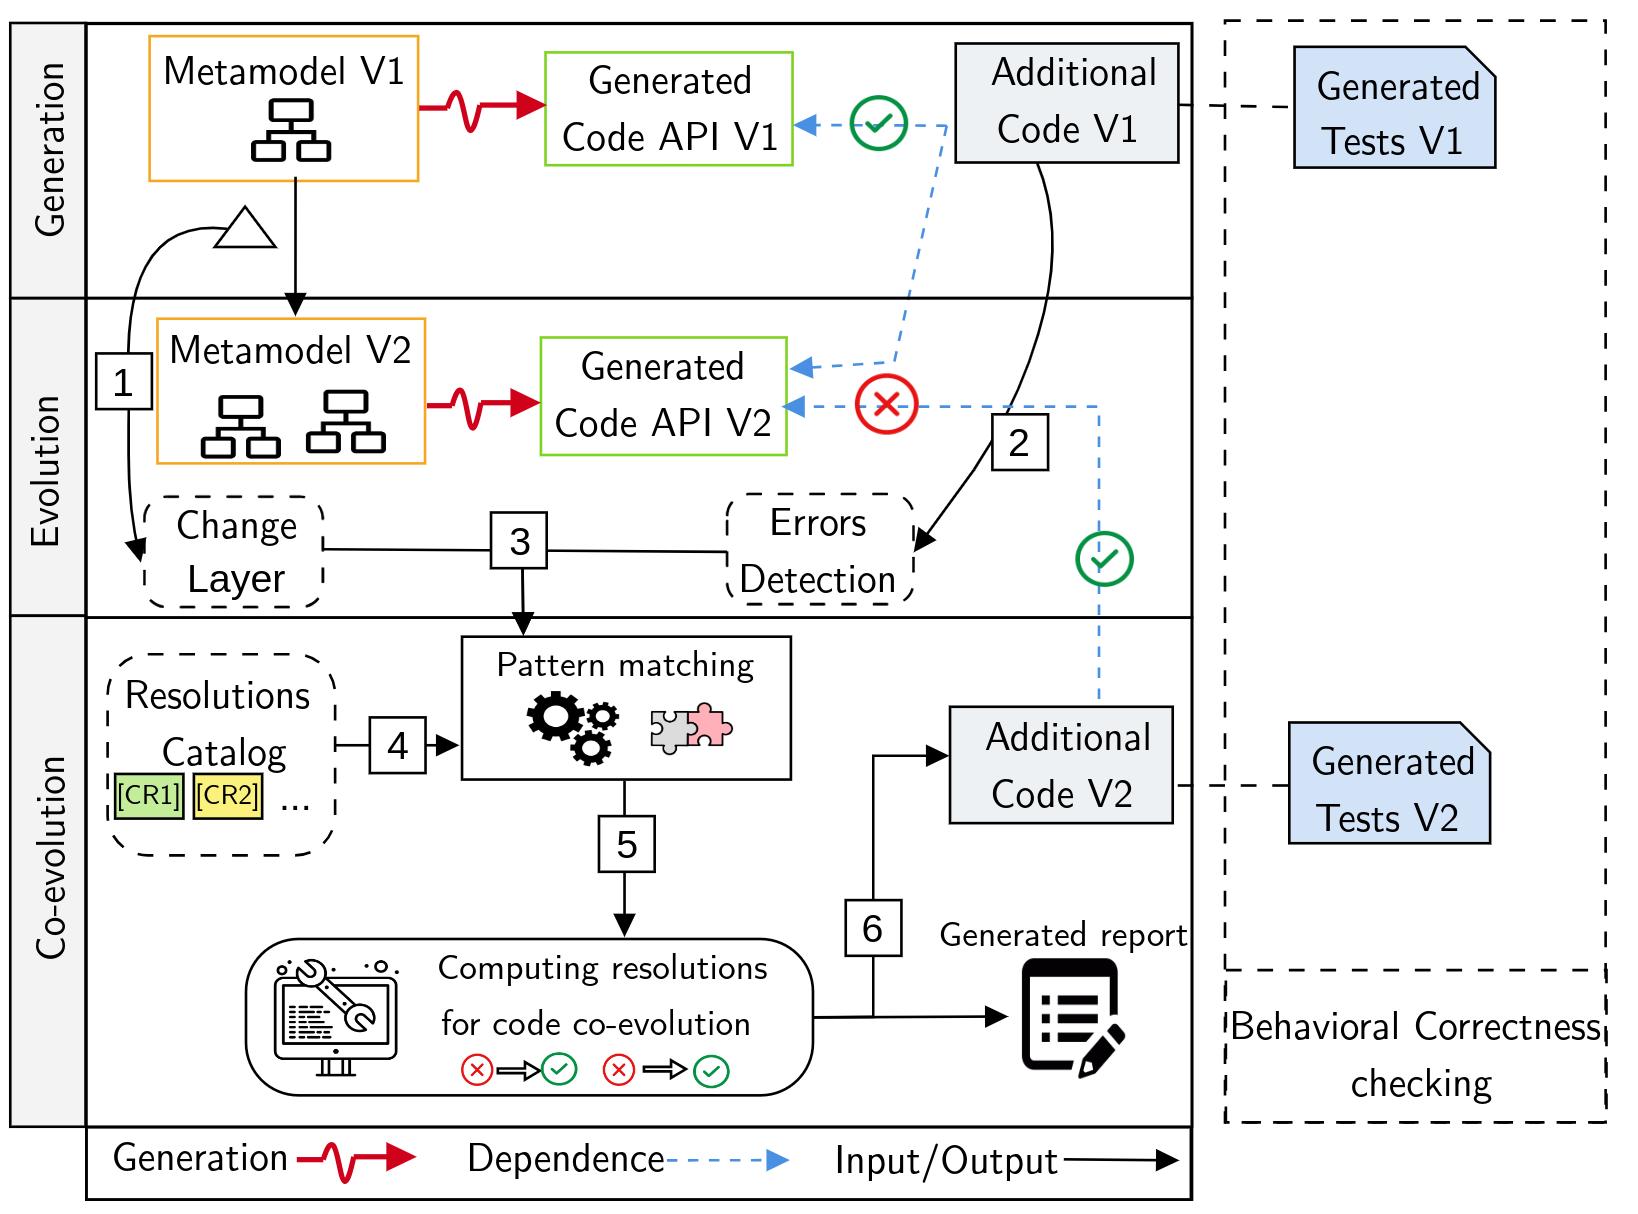
\includegraphics[width=0.8\textwidth]{./pics/chapter1pics/ApproachV5.png}
	\caption{Overall approach for metamodel and code co-evolution}
	\label{fig:overallapproach}
	%\vspace{-1em}
	\vspace{-1em}
\end{figure*}
%\end{wrapfigure}
%\section{Change detection}
\label{sec: ap1_changedetection}

\section{Motivating Example}\label{example}

This section introduces a motivating example to illustrate the challenge of metamodel and code co-evolution. 
Let us take as an example the Modisco project \cite{MDTModisco}, which has evolved numerous times in the past. Modisco is an academic initiative project implemented in the Eclipse platform to support the development of model-driven tools, reverse engineering, verification, and transformation of existing software systems \cite{bruneliere2010modisco,bruneliere2014modisco}.


Figure \ref{fig: BMM} shows an excerpt of the "Modisco Discovery Benchmark" metamodel\footnote{\url{https://git.eclipse.org/r/plugins/gitiles/modisco/org.eclipse.modisco/+/refs/tags/0.12.1/org.eclipse.modisco.infra.discovery.benchmark/model/benchmark.ecore}} consisting of 10 classes in version~0.9.0.
It illustrates some of the domain concepts \textbf{Discovery}, \textbf{Project}, and \textbf{ProjectDiscovery}  used for the discovery and reverse engineering of an existing software system. 
From these metaclasses, a first code API is generated, containing Java interfaces and their implementation classes, a factory, a package, etc. Listing \ref{lis:Modisco_Code_API_V1} shows a snippet of the generated Java interfaces and classes from the metamodel in Figure \ref{fig: BMM}. 

The generated code API is further enriched by the developers with additional code functionalities in the "Modisco Discovery Benchmark" project and its dependent projects as well.
For instance, by implementing the methods defined in metaclasses and advanced functionalities in new classes. Listing \ref{lis:Modisco_Code_External_V1} shows the two classes \texttt{Report} and \texttt{CDOProjectDiscoveryImpl} of the additional code in the same project "Modisco Dsicovery Benchmark" and in another dependent project, namely the "Modisco Java Discoverer Benchmark" project. 
In version~0.11.0, the "Modisco Discovery Benchmark" mesloppypar package installtamodel evolved with several significant changes, among which the following impacting changes:

\begin{enumerate}%[noitemsep,nolistsep]
	
	\item Deleting the metaclass \texttt{ProjectDiscovery}. 
	
	\item Renaming the property \emph{totalExecutionTimeInSeconds} to \emph{discoveryTimeInSeconds} in metaclass \texttt{Discovery}. 
	
	\item Moving the property \emph{discoveryTimeInSeconds} (after its rename) from metaclass \texttt{Discovery} to \texttt{DiscoveryIteration}. 
	
\end{enumerate} 


\begin{figure}
	
	\centering
	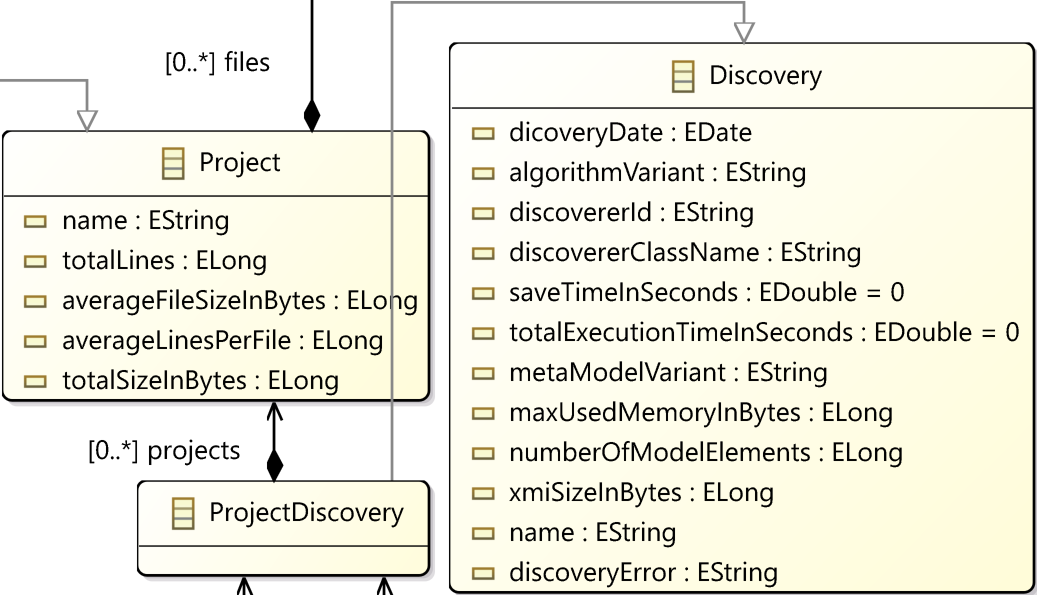
\includegraphics[width=0.48\textwidth]{pics/chapter1pics/example.PNG}
	\caption{Excerpt of Modisco Benchmark metamodel in version 0.9.0.}
	\label{fig: BMM}
	\vspace{-5mm}
\end{figure}

After applying these metamodel changes, naturally, the code of Listing \ref{lis:Modisco_Code_API_V1} is regenerated from the evolved version of the metamodel, which in turn impacts the existing additional code depicted in Listings \ref{lis:Modisco_Code_External_V1}. 
The resulting errors in the original code in version 0.9.0 are underlined in red in Listing \ref{lis:Modisco_Code_External_V1}. 
Listing \ref{lis:Modisco_Code_External_V2} presents the final result of the co-evolution process in version 0.11.0. The co-evolved code is underlined in green. 
For example, in response to the \textit{delete} of the metaclass \texttt{ProjectDiscovery}, its import statement {\small\boxed{Line~1}} in Listing \ref{lis:Modisco_Code_External_V1}, and any usage of it or its methods are impacted. The import statement is completely removed. The same can be applied to the usages of the class and its methods. Alternatively, they could also be replaced by a default value rather than removing the whole instruction. The intention is to maintain the developers' code with minimal removal co-evolution. 

Furthermore, the same changes \textit{rename} and \textit{move} of the property \emph{totalExecutionTimeInSeconds} impact two usages that are co-evolved differently. First, the call of \texttt{setTotalExecutionTimeInSeconds} ({\small\boxed{Line~4}} in Listing~\ref{lis:Modisco_Code_External_V1}) that is co-evolved by renaming it to \texttt{setDiscoveryTimeInSeconds}, then extending the path with \texttt{getIterations()}. The second impact is the use of the generated literal %\texttt{BenchmarkPackage.}\emph{\footnotesize{DISCOVERY\_\_TOTAL\_EXECUTION\_TIME\_IN\_SECONDS}}. It is successively co-evolved by renaming it to \texttt{BenchmarkPackage.}\emph{\footnotesize{DISCOVERY\_\_DISCOVERY\_TIME\_IN\_SECONDS}} before replacing its source class \texttt{DISCOVERY} by \texttt{DISCOVERY\_ITERATION}. 
\texttt{\footnotesize{BenchmarkPackage.DISCOVERY\_\_TOTAL\_EXECUTION\_TIME\_IN\_SECONDS}}. It is successively co-evolved by renaming it to \texttt{\footnotesize{BenchmarkPackage.DISCOVERY\_\_DISCOVERY\_TIME\_IN\_SECONDS}} before replacing its source class \texttt{DISCOVERY} by \texttt{DISCOVERY\_ITERATION}. 
Note that when using the IDE quick fixes to co-evolve these errors, it suggests to create the method \texttt{setTotalExecutionTimeInSeconds} in the class \texttt{Discovery} and the literal \emph{\footnotesize{DISCOVERY\_\_TOTAL\_EXECUTION\_TIME\_IN\_SECONDS}} in the class \texttt{BenchmarkPackage}, which does not meet the required co-evolutions shown in Listing~\ref{lis:Modisco_Code_External_V2}.

The above examples show the importance of correctly matching the different code usages and patterns of the generated code elements with the metamodel evolution changes to co-evolve them with the appropriate resolutions. 

The next section presents our contribution for a fully automatic co-evolution of metamodel and code.  

\begin{lstlisting}[language=Java,breaklines=true,mathescape,literate={\-}{}{0\discretionary{-}{}{}},caption=excertprpt of the generated code in org.eclipse.modisco.infra.discovery.benchmark.\label{lis:Modisco_Code_API_V1}]
	//Discovery Interface
	public interface Discovery extends EObject {
		double getTotalExecutionTimeInSeconds();
		void setTotalExecutionTimeInSeconds(double value);
		...
	}
	//Project Interface
	public interface ProjectDiscovery extends Discovery {...}
	//DiscoveryImpl Class
	public class DiscoveryImpl extends EObjectImpl implements Discovery {
		public double getTotalExecutionTimeInSeconds() {...}
		public void setTotalExecutionTimeInSeconds(double totalExecTime) {...}
		...
	}
\end{lstlisting}
%xleftmargin=0.2cm,xrightmargin=0cm,framexleftmargin=+6pt,frame=single,
\begin{lstlisting}[language=Java,breaklines=true,mathescape,literate={\-}{}{0\discretionary{-}{}{}},caption=Excerpt of the additional code V1.\label{lis:Modisco_Code_External_V1}]
	import (*{\scriptsize org.eclipse.modisco.infra.discovery.benchmark}*).(*\ul{\scriptsize ProjectDiscovery}*);
	public class Report {
		...
		discovery.(*\ul{setTotalExecutionTimeInSeconds}*)(...);
	}
	...
	public class CDOProjectDiscoveryImpl extends AbstractCDODiscoveryImpl implements CDOProjectDiscovery {
		...
		case JavaBenchmarkPackage.
		CDO_PROJECT_DISCOVERY__TOTAL_EXECUTION_TIME_IN_SECONDS: return BenchmarkPackage.
		(*\ul{DISCOVERY\_\_TOTAL\_EXECUTION\_TIME\_IN\_SECONDS}*);
		...
	}
	
	
\end{lstlisting}

\begin{comment}
	public class JavaDiscoveredProjectImpl extends AbstractJavaProjectImpl implements JavaDiscoveredProject {
		
		public int eBaseStructuralFeatureID(int derivedFeatureID, Class<?> baseClass) {
			...
			case JavaBenchmarkPackage.JAVA_DISCOVERED_PROJECT__DISCOVERIES: return BenchmarkPackage.
			(*\ul{DISCOVERED\_PROJECT\_\_DISCOVERIES}*);
			...
		}
		...
	}
\end{comment}
%%%%%%%%%%%%%%%%%%%%%%%%%%%%%%%%%%%%%%%%%%%%%%%%%%%%%%%%%%%
%%                   Now the evolved code                %%
%%%%%%%%%%%%%%%%%%%%%%%%%%%%%%%%%%%%%%%%%%%%%%%%%%%%%%%%%%%
\setulcolor{green} 
\setstcolor{green}
%\setstcolor{green}
%,xleftmargin=0.2cm,,xrightmargin=-0cm,framexleftmargin=+6pt,frame=single
\begin{lstlisting}[language=Java,breaklines=true,mathescape,literate={\-}{}{0\discretionary{-}{}{}},caption=Excerpt of the additional code V2.\label{lis:Modisco_Code_External_V2}]
	(*{\st{import }}*)(*{\scriptsize \st{ org.eclipse.modisco.infra.discovery.benchmark. ProjectDiscovery}}*);
	public class Report {
		...
		discovery.(*\ul{getIterations().}*) 
		(*\ul{setDiscoveryTimeInSeconds}*)(...);
		...
	}
	public class CDOProjectDiscoveryImpl extends AbstractCDODiscoveryImpl implements CDOProjectDiscovery {
		...
		case JavaBenchmarkPackage.
		CDO_PROJECT_DISCOVERY__TOTAL_EXECUTION_TIME_IN_SECONDS: return BenchmarkPackage.
		(*\ul{DISCOVERY\_ITERATION\_\_DISCOVERY\_TIME\_IN\_SECONDS}*);
		...
	}
	...
}
\end{lstlisting}
%\begin{lstlisting}[language=Java,breaklines=true,mathescape,literate={\-}{}{0\discretionary{-}{}{}},xleftmargin=0.2cm,xrightmargin=-0.4cm,framexleftmargin=+6pt,frame=single,caption=Excerpt of the additional external code in the SL org.eclipse.modisco.infra.discovery.benchmark.\label{lis:Modisco_Code_External_V1}]

\begin{comment}
....
public class JavaDiscoveredProjectImpl extends AbstractJavaProjectImpl implements JavaDiscoveredProject {
	public int eBaseStructuralFeatureID(int derivedFeatureID, Class<?> baseClass) {
		...
		case JavaBenchmarkPackage.JAVA_DISCOVERED_PROJECT__DISCOVERIES: return BenchmarkPackage.(*\ul{BENCHMARK\_\_DISCOVERIES}*);
		...
	}
	...
}
\end{comment}



\section{Approach}\label{approach}

This section presents the overall approach of our automated co-evolution of code with evolving metamodels,  instantiating on the Ecore technological space. First, we give an overview of the approach and specify the metamodel evolution changes we consider. 
%
Then, we present how we retrieve the resulting errors due to metamodel evolution, followed by the regeneration of the code API. 
After that, we present the pattern matching process, which is an important part of our fully automatic co-evolution approach, before discussing the resolutions of the code errors. 

\subsection{Overview}
\label{Overview}
Figure~\ref{fig:overallapproach} depicts the overall steps for the automatic co-evolution of the metamodel and code, with horizontally separated parts defining chronological order from the top to the bottom.
%\\
After the generation step (the upper part of Figure~\ref{fig:overallapproach}), the evolution of the Ecore metamodel will cause errors in the additional Java code that depends on the API of the newly generated code (the middle part of Figure~\ref{fig:overallapproach}). We take as input the evolution changes of the metamodel between the two versions of this metamodel {\small\boxed{1}}. Then, we parse the additional code  {\small\boxed{2}} to retrieve the list of errors. 
After that, we get to the bottom part of Figure~\ref{fig:overallapproach}, both the list of metamodel changes and the list of errors are used as inputs for the \red{pattern matching step {\small\boxed{3}}. It analyzes the structure of the error to match it with its impacting metamodel change and decides which resolution  {\small\boxed{4}} to apply for the error co-evolution {\small\boxed{5}}. The metamodel changes provide the ingredients and necessary information that are used for the co-evolution.  
	At the end of the automatic co-evolution, we obtain a new co-evolved additional code {\small\boxed{6}} along a generated report on the applied resolutions.} 
In addition to the automatic co-evolution, we generate test cases before and after co-evolution to highlight its possible effect. In fact, many research papers rely on the use of tests to check the behavior of the code during its evolution. For example, Godefroid et al.~\cite{10.1145/3395363.3397374} uses tests to find regressions in different versions of REST APIs. In particular, Lamothe et al.~\cite{9079197},~\cite{10.1145/3387905.3388608} use tests to validate the evolution of the client code after Android API migration. We apply a similar method to check the effect of the co-evolution. 
Finally, during the co-evolution process, we generate a report linking the applied resolutions for each code error with its impacting metamodel change. If needed, this can help developers in understanding the performed co-evolution, since we fully automate it.
%\todo{refs behavioral check et papier android : to check}
%\DK{we see later if we add the story of generated tests after co-evolution}

\subsection{Metamodel Evolution Changes}
\label{mmchanges}

One of the intrinsic properties of software artifacts is its continuous evolution~\cite{mens2008introduction}. Metamodels are no different and are meant to evolve. 
Two types of evolution changes are considered when evolving a metamodel: \emph{atomic} and \emph{complex} changes~\cite{Herrmannsdoerfer2011}. 
Atomic changes are additions, removals, and updates of a metamodel element. Complex changes consist of a sequence of atomic changes combined together~\cite{vermolen_reconstructing_2012},~\cite{khelladi2015detecting}. For example, move property is a complex change where a property is moved from a source class to a target class. This is composed of two atomic changes: delete property and add property~\cite{Herrmannsdoerfer2011}. 
Many approaches in the literature~\cite{Alter2015, williams2012searching,cicchetti_managing_2009,langer_posteriori_2013,vermolen_reconstructing_2012,Khelladi2016,bettini2022executable} exist to detect metamodel changes between two versions. Note that the detected list of complex changes does not include the list of the detected atomic changes, i.e., no overlap in between. 
\red{Moreover, the detection approaches must order the changes in a consistent way. This is fundamentally a problem that change detection approaches must deal with, and hence, is out of scope for our problem of code co-evolution. Nonetheless, it is important and expect a consistent order of changes to not hinder the quality of the co-evolution.}

For the purpose of modularity and extensibility, we use a specification layer for the changes~{\small\boxed{1}} that is simply a connection layer to our co-evolution approach with existing change detection approaches. This connection layer specifies our own representation of a metamodel change that can be mapped later with any change representation. \red{It simply specifies the needed information for each change in the form of its attributes. In the left column of Table \ref{table:ResolutionsCatalog}, we precise the impacting changes that we consider in our work. For each change, we precise in the second column the attributes that represent and compose each change. When using a state-of-the Art detection approach, we analyze in white box the detected changes to extract their attributes and map them to our internal change layer.
	%the attributes of each change are mapped with the corresponding detected change. In order to map the output changes of the used detection approach, we analyze in white box their results to retrieve their different attributes and map them with our change layer.
} 
For example, a rename property change includes information regarding its old name, new name, and its class container. Therefore, in practice, any detection approach~\cite{Alter2015, williams2012searching,cicchetti_managing_2009,langer_posteriori_2013,vermolen_reconstructing_2012,Khelladi2016,bettini2022executable} can be integrated by bridging its changes' representation to our change layer and the rest of co-evolution can be performed independently.
In this approach, we chose to reuse our previous work \cite{Khelladi2016}, a heuristic-based approach to actually detect atomic and complex changes between two versions of a metamodel.
In the rest of the chapter, we focus on the code co-evolution since it is our main contribution. 

\subsection{Error Retrieval}
\label{errorretrieving}

After the metamodel is evolved and the code API is re-generated, errors will appear in the additional code that must be co-evolved. Unlike code migration context~\cite{9079197},~\cite{henkel2005catchup}, these errors represent the delimited impact of the metamodel evolution. Thus, rather than an impact analysis on the original version to trace the impact of a metamodel change in the code, our approach relies on the compilation result of the code to retrieve its errors. 
This is necessary and useful in our approach, as we will need to keep updating the list of code errors after co-evolving each given error, hence, iteratively co-evolving the code. We detail this process in the following subsections.

To retrieve those errors, we start by parsing the code of each Java class, called a \emph{compilation unit}, to access the Abstract Syntax Trees (ASTs). An error in a Java code is called a \emph{Marker} that contains the information regarding the detected error. It contains the necessary information to locate the exact impacted AST node in the parsed global AST (\ie char start and end) and  to process it (\ie message).
In the remaining part of the chapter, instead of Markers, compilation units, and additional code, we respectively refer only to errors, Java classes, and code for the sake of simplicity.  

\subsection{Resolution Catalog}

Now that we have a list of code errors, we need a set of resolutions to co-evolve them.
\blue{Our co-evolution approach relies on the resolutions shown in Table \ref{table:ResolutionsCatalog}. 
	%
	%Table \ref{table:ResolutionsCatalog} 
	It depicts the resolutions associated with metamodel changes that are known to have an impact on code \cite{iovino2012impact}.
	The resolutions are taken from existing co-evolution approaches of various MDE artifacts \cite{kessentini2018integrating,kessentini2019automated,cicchetti2008automating,herrmannsdoerfer2009cope,garces2009managing,wachsmuth2007metamodel,batot2017heuristic,khelladi2017semi,correa2007refactoring,kessentini2018automated,khelladi2018change,garces2014adapting,garcia2013model,kusel2015consistent,kusel2015systematic,hebig2015surveying}, % or constraints \cite{khelladi2017semi}
	where they showed to be efficient and useful in co-evolving code \cite{Khelladi2020}.
	
	For example, resolutions $[CR8,CR9, CR10, CR11]$   aim to co-evolve the different code errors of a move property in the metamodel. %We notice that a metamodel change can be treated by more than one resolution, so how do we select one resolution per change? [or the following paragraph presents our solution to select one resolution per change.]
}


\begin{sidewaystable}


	%\setlength\extrarowheight{1pt}
%\begin{table*}[t]
	%\vspace{-1.5em}
	\centering

	\caption{Catalog of resolutions used for the code co-evolution of direct errors due to the metamodel changes.}
	\label{table:ResolutionsCatalog}
	\resizebox{22.5cm}{!} {
	%	\vspace{-4cm}
			\hspace{-1cm}

		\begin{tabular}{lll}
			\toprule
			\begin{tabular}[c]{@{}l@{}}Impacting Metamodel Changes\end{tabular} 
			&  \begin{tabular}[c]{@{}l@{}}Changes' attributes\end{tabular} 
			& \begin{tabular}[c]{@{}c@{}}Proposed Code Resolutions\end{tabular}   
			
			\\ \midrule
			
			
			
			%			* 0 to delete the instruction where the deleted method is used, 
			%			* 1 delete the direct element only 
			%			* 2 delete the direct expression (all call path) using this deleted property 
			%			* 3 replace the direct expression (all call path) with a default value
			%			* 4 replace it with another element (like rename)
			
			\begin{tabular}[c]{@{}l@{}}	$\diamond$ Delete property \emph{p} \\from class \emph{C}\end{tabular} 
			&  \begin{tabular}[c]{@{}l@{}}	$\circ$ Property \emph{p} name \\ $\circ$ Container class \emph{C} name\end{tabular} &  
			\begin{tabular}[c]{@{}l@{}}$\rhd [CR1]$ Remove the direct use of \emph{p} \red{}(e.g., label = s.name + s.m1().p.m2() $\rightarrow$ label = s.name + ( (Type\_Of\_P) s.m1() ).m2())\\
				$\rhd [CR2]$ Remove the statement using \emph{p} (i.e., if, loop, assignment, etc.) \\
				$\rhd [CR3]$ Remove the whole call path of \emph{p} (e.g., label = s.name + s.m1().m2().p $\rightarrow$ label = s.name) \\
				$\rhd [CR4]$ Replace the whole call path of \emph{p} with a default value (e.g., id = s.id + s.m1().m2().p $\rightarrow$ id = s.id + 0) 
				
			\end{tabular}    \\ \midrule
			
			$\diamond$ Delete class \texttt{C} 
			& \begin{tabular}[c]{@{}l@{}}$\circ$ Class \emph{C} name \\ $\circ$ Container package \emph{Q} name\end{tabular} 
			& \begin{tabular}[c]{@{}l@{}}$\rhd [CR1]$ Remove the direct use of the type \texttt{c} (e.g., extending/implementing \texttt{c}, in method argument/returned \\ type and not the whole method declaration. Calls to the updated methods are subsequently updated) \\%\textcolor{white}{-----------}
				$\rhd [CR2]$ Remove the statements using the type \texttt{C} (e.g., import, variable declaration, method argument/returned type, \\ method declaration,  type instantiation, etc. Calls to the deleted variables and methods are subsequently removed)\\%\textcolor{white}{-----------}
				
			\end{tabular} 	  \\ \midrule
			
			$\diamond$ Rename element \emph{e} to \emph{e'}
			& \begin{tabular}[c]{@{}l@{}}	$\circ$ Element \emph{e} old name \\$\circ$ Element \emph{e'} new name \\$\circ$ Container package \emph{Q} or class \emph{C} name\end{tabular}
			& \begin{tabular}[c]{@{}l@{}} $\rhd [CR5]$ Rename \emph{e} in the code	
			\end{tabular}
			\\
			\midrule
			
			\begin{tabular}[c]{@{}l@{}}$\diamond$ Generalize multiplicity of \\ property \emph{p} of the class \emph{C} from \\ a single to multiple values\end{tabular} 
			& \begin{tabular}[c]{@{}l@{}}	$\circ$ Property \emph{p} name \\ $\circ$ Container Class  \emph{C} \\ $\circ$ Old multiplicity
				\\ $\circ$ New multiplicity\end{tabular} 
			& 
			\begin{tabular}[c]{@{}l@{}}
				$\rhd [CR6]$ Retrieve the first value of a collection (e.g., value = \emph{lng.p}  $\rightarrow$ value = \emph{lng.p.toArray()[0]} or \emph{lng.p.get(0)} )\\
				
			\end{tabular}   \\ \midrule
			
			%			* 0 extend navigation path
			%			* 1 reduce navigation path
			%			* 2 extend a navigation path and add a loop
			%			* 3 extend a navigation path and get the first/last/i^th element
			%			* 4 replace reference in path call x.y.z.prop to x.y.w.prop
			
			\begin{tabular}[c]{@{}l@{}}$\diamond$ Move property $p_{i}$ from \\ class \texttt{S} to \texttt{T} through \emph{ref}\\
				%$\diamond$ Extract class \texttt{S} to \texttt{T} \\with properties $p_{1},...,p_{n}$ \\ \red{through \emph{ref}}\\
				$\diamond$ Extract class of properties $p_{1},$\\$...,p_{n}$ from \texttt{S} to \texttt{T} through \emph{ref}\end{tabular}
			& \begin{tabular}[c]{@{}l@{}} $\circ$ Property \emph{p} name \\ $\circ$ Source container class \emph{S} name \\$\circ$  Target container class \emph{T} name \\$\circ$ Reference \emph{ref} name \end{tabular} 
			& 
			\begin{tabular}[c]{@{}l@{}}$\rhd [CR7]$ Extend navigation path of $p_{i}$ (e.g., \emph{lng.$p_{i}$}  $\rightarrow$ \emph{lng.ref.$p_{i}$})\\
				
				$\rhd [CR8]$ Extend navigation path of $p_{i}$ and add a for loop (e.g., \emph{lng.$p_{i}$}  $\rightarrow$ \emph{for(v in lng.ref) \{v.$p_{i}$\}})\\
				$\rhd [CR9]$ Reduce navigation path of $p_{i}$ (e.g., \emph{lng.ref.$p_{i}$}  $\rightarrow$ \emph{lng.$p_{i}$})\\
				$\rhd [CR10]$ Replace S by T\_REF  in Literal values (e.g., \emph{MetamodelPackage.S\_\_$p_{i}$}  $\rightarrow$ \emph{MetamodelPackage.T\_\_$p_{i}$})
			\end{tabular}   \\ \midrule
			
			\begin{tabular}[c]{@{}l@{}}$\diamond$ Push property \emph{p} from \\class \texttt{Sup} to \texttt{Sub$_{1}$},...,\texttt{Sub$_{n}$}\end{tabular} 
			& \begin{tabular}[c]{@{}l@{}}	$\circ$ Property \emph{p} name \\ $\circ$ Container class \emph{Sup} name \\ $\circ$ List of container classes \emph{Sub$_{i}$} names
			\end{tabular} 
			& 
			\begin{tabular}[c]{@{}l@{}}$\rhd [CR11]$ Introduce a type test with an If statement (e.g., \emph{t.name = s.p.name} $\rightarrow$ \\$if(s.p.istypeof(Sub_{1})$) \{t.name = (Sub$_{1}$ s).p.name\} $...$ $else$ $if(s.p.istypeof(Sub_{n})$ \{t.name = (Sub$_{n}$ s).p.name\})\\
				$\rhd [CR12]$ Cast \emph{p} to one specific sub class $Sub_{i}$ (e.g., \emph{t.name = s.p.name} $\rightarrow$ \emph{t.name = (($Sub_{i}$)s).p.name})\\
				$\rhd [CR13]$ Duplicate the statement using the literal for each subclass and replace Sup by $Sub_{i}$ (e.g., \emph{add(Package.Sup\_\_P)} \\ $\rightarrow$ \emph{ add(Package.$Sub_{0}$\_\_P)}, ... , \emph{add(Package.$Sub_{n}$\_\_P)})
				%Create much Literals as subclasses and replace Sup by $Sub_{i}$ in each one(e.g., \emph{MetamodelPackage.Sup\_\_P}  $\rightarrow$ \emph{lng.$Sub_{0}$\_\_P} ,...,\emph{lng.$Sub_{n}$\_\_P})
			\end{tabular}   \\ \midrule
			\begin{tabular}[c]{@{}l@{}}$\diamond$ Pull property \emph{p} from \\classes \texttt{Sub$_{1}$},...,\texttt{Sub$_{n}$}
				to \texttt{Sup}  \end{tabular} 
			& \begin{tabular}[c]{@{}l@{}}		$\circ$ Property \emph{p} name \\ $\circ$ List of container classes \emph{Sub$_{i}$}  \\ $\circ$ Container class \emph{Sup} name\end{tabular} 
			& 
			\begin{tabular}[c]{@{}l@{}}
				%$\rhd [CR12]$ Cast \emph{p} to sup  (e.g., \emph{t.name = s.p.name} $\rightarrow$ \emph{t.name = ((Sup)s).p.name})\\
				$\rhd [CR14]$ Replace $Sub_{i}$  by Sup in Literal values (e.g., \emph{MetamodelPackage.$Sub_{i}$\_\_P}  $\rightarrow$ \emph{MetamodelPackage.Sup\_\_P})
				
			\end{tabular}   \\ \midrule
			
			%			\begin{tabular}[c]{@{}l@{}}$\diamond$ Extract class \texttt{S} to \texttt{T} \\with properties $p_{1},...,p_{n}$\end{tabular} & 
			%			\begin{tabular}[c]{@{}l@{}}$\rhd [CR10]$ Extend navigation path of $p_{i}$ (e.g., \emph{lng.$p_{i}$}  $\rightarrow$ \emph{lng.path.$p_{i}$})\\
				%				$\rhd [CR11]$ Reduce navigation path of $p_{i}$ (e.g., \emph{lng.path.$p_{i}$}  $\rightarrow$ \emph{lng.$p_{i}$}) \end{tabular}   \\ \midrule
			
			%			
			
			
			\begin{tabular}[c]{@{}l@{}}$\diamond$ Inline class \texttt{S} to \texttt{T} \\with properties $p_{1},...,p_{n}$\end{tabular} 
			& \begin{tabular}[c]{@{}l@{}}   $\circ$ List of properties \emph{p$_{i}$}  \\$\circ$ Container Source class \emph{S} name \\ $\circ$ Container Target class \emph{T} name\end{tabular} 
			& 
			%delete rule or change its source/target type from B to A
			\begin{tabular}[c]{@{}l@{}}
				$\rhd [CR9]$ Reduce navigation path of $p_{i}$ (e.g., \emph{lng.ref.$p_{i}$}  $\rightarrow$ \emph{lng.$p_{i}$})\\
				$\rhd [CR15]$ Change the class type from \texttt{S} to \texttt{T} \red{}(e.g., List$<$S$>$ l = ...; $\rightarrow$ List$<$T$>$ l = ...; ) \\
			\end{tabular} \\ \midrule
			
			%			\begin{tabular}[c]{@{}l@{}}$\diamond$ Flatten hierarchy from \\class \texttt{Sup} to \texttt{Sub$_{1}$},...,\texttt{Sub$_{n}$}\\with properties $p_{1},...,p_{n}$\end{tabular} & 
			%			%delete rule of change its source/target type from A to B1 ... Bn
			%			\begin{tabular}[c]{@{}l@{}}$\rhd [R15]$ Duplicate the transformation rule while changing the source or target class type from \texttt{Sup} to \texttt{Sub$_{i}$} ($i \in [1...n] $)  \\
				%				$\rhd [CR3]$ Remove the whole transformation rule \\ \end{tabular}  \\ 
			\begin{tabular}[c]{@{}l@{}}$\diamond$ Change property \emph{p} type \\ of the class \emph{C} from \texttt{S} to \texttt{T}\end{tabular}
			& \begin{tabular}[c]{@{}l@{}}	$\circ$ Property \emph{p} name \\ $\circ$ Container class \emph{C} name \\ $\circ$ Old type \emph{S}\\ $\circ$ New type \emph{T} \end{tabular} 
			& 
			\begin{tabular}[c]{@{}l@{}}$\rhd [CR16]$ Change variable declaration type initialized with \emph{p} from \texttt{S} to \texttt{T} (e.g., S var = s.p; $\rightarrow$ T var = s.p;) \\ $\rhd [CR17]$ Add a cast of \emph{p} 
			\end{tabular}   \\ %\midrule
			\bottomrule  
			
			                
		\end{tabular}
				
}
%\end{adjustbox}	
\end{sidewaystable}	
%\end{table*}


\subsection{Pattern Matching for Resolution Selection}
\label{pattern_matching}



\begin{table*}[t]
	
	\caption{Classification of the different patterns of the generated code element from the metamodel elements.} 
	\label{table:locationofMMelemen_ch1}
	\hspace{-1cm}
	\resizebox{19cm}{!} {
		{\small
			\begin{tabular}{llll}
				\toprule
				
				\begin{tabular}[c]{@{}l@{}} \textbf{Metamodel}\\ \textbf{element type} 
				\end{tabular} & \textbf{Generated code elements}& \textbf{Pattern of the generated code elements}& \textbf{Illustrative examples}\\ \midrule
				
				
				\multirow{6}{*}{Metaclass} & Interface & "MetaClassName" & \textit{Constraint} \\ \cline{2-4} 
				& \begin{tabular}[c]{@{}l@{}}createClass() \\ (in metamodelFactory class)\end{tabular} & "create"+"MetaClassName"() &\textit{createConstraint()} \\ \cmidrule{2-4} 
				& \begin{tabular}[c]{@{}l@{}}Literals of the class \end{tabular} &
				\begin{tabular}[c]{@{}l@{}}
					"META\_CLASS\_NAME"\\
					"META\_CLASS\_NAME"+"\_"+ "FEATURE\_COUNT"\\
					"META\_CLASS\_NAME"+ "\_"+"OPERATION\_COUNT"
				\end{tabular} 
				& \begin{tabular}[c]{@{}l@{}}\textit{CONSTRAINT}, \\ \textit{CONSTRAINT\_FEATURE\_COUNT}, \\  \textit{CONSTRAINT\_OPERATION\_COUNT}\end{tabular} \\ \cmidrule{2-4} 
				& \begin{tabular}[c]{@{}l@{}}Accessor of Meta objects \\ (in metamodelPackage class)\end{tabular} & "get"+"MetaClassName"()& \textit{getConstraint() }\\ \cmidrule{2-4} 
				& Class implementation & "MetaClassNameImpl" &\textit{ConstraintImpl }\\ \cmidrule{2-4} 
				& Adapter & "create"+"MetaClassName"+"Adapter" & \textit{createConstraintAdapter()} \\ \midrule
				
				
				\multirow{1}{*}{Attribute} & Signature of getters and setters & "get"+"AttributeName"(), "set"+"AttributeName"()& \textit{getStereotype()}, \textit{setStereotype() }\\ \cmidrule{2-4} 
				\multirow{3}{*}{(same for a reference)} & Accessor of Meta objects &"get"+"MetaClassName"+"\_"+"AttributeName"() &\textit{ getConstraint\_Stereotype()} \\ \cmidrule{2-4} 
				& Literal & "META\_CLASS\_NAME"+"\_\_"+"ATTRIBUTE\_NAME"& \textit{CONSTRAINT\_\_STEREOTYPE} \\ \cmidrule{2-4} 
				& \begin{tabular}[c]{@{}l@{}}Implementation \\ of getters and setters\end{tabular} &"get"+"AttributeName"(), "set"+"AttributeName"()& getStereotype(), setStereotype() \\ \midrule
				
				
				\multirow{4}{*}{Method} & Declaration of the method& "methodName"()& \textit{UniqueName() }\\ \cmidrule{2-4} 
				& Accessor of meta objects &"get"+"MetaClass"+"\_\_"+"MethodName"()& \textit{getCONSTRAINT\_\_UniqueName() }\\ \cmidrule{2-4} 
				& Literal &"META\_CLASS\_NAME"+"\_\_"+"METHOD\_NAME"& \textit{CONSTRAINT\_\_\_UNIQUE\_NAME }\\ \cmidrule{2-4} 
				& Implementation of the method &"methodName"()& \textit{UniqueName()} \\ %\midrule
				
				
				%\multirow{4}{*}{Reference} & Accessor of meta objects &"get"+"MetaClassName"+"\_"+"ReferenceName"()& \textit{getConstraint\_ConstraintElement()} \\ \cmidrule{2-4} 
				% & Signature of getters and setter & "get"+"ReferenceName"(),"set"+"ReferenceName"()&\textit{ getConstraintElement()}, \textit{setConstraintElement() }\\ \cmidrule{2-4} 
				% & Literal &"META\_CLASS\_NAME"+"\_\_"+"REFERENCE\_NAME"& \textit{CONSTRAINT\_\_CONSTRAINT\_ELEMENT} \\ \cmidrule{2-4} 
				% & \begin{tabular}[c]{@{}l@{}}Implementation of \\ getters and setters\end{tabular} &"get"+"ReferenceName"(), "set"+"RegerenceName"()& \textit{getConstraintElement()}, \textit{setConstrainElement() }\\ 
				\bottomrule
				
				%cline hline replaced with cmidrule and midrule
				
			\end{tabular}
		}
	}
\end{table*}

As shown in Table \ref{table:ResolutionsCatalog}, alternative resolutions exist per metamodel change. Since we aim to fully automate the co-evolution, we need a mechanism to analyze the code error, the code usage, and its impacting metamodel change to decide which resolution to apply. 
This section presents the pattern matching process between metamodel changes and code usages for the retrieved code errors to automatically select resolutions for their co-evolution.

Each Metamodel Element $ME$ has corresponding Generated Code Elements \{$GCE_0$, $GCE_1$, ..., $GCE_n$\} in the code API. 
$GCE_i$ have \textbf{usages} in the \textbf{additional code} as illustrated in Figure~\ref{fig:patternconcept}.
Thus, evolving a $ME$ will regenerate \{$GCE_0$, $GCE_1$, ..., $GCE_n$\} which will impact their \textbf{usages}. 
%
Table~\ref{table:locationofMMelemen} classifies the different patterns of the generated code elements $GCE_i$ for each metamodel element $ME$ type, and provides illustrative examples. It shows that various patterns of code elements are generated for each metamodel element type. % and with different patterns. 
%mapping between the different metamodel elements and their corresponding generated code elements with illustrative examples. 
For example, let us consider the case of a metaclass. EMF generates a corresponding interface and a class implementation, a \emph{createClass()} method in the factory class, three literals (\ie constants) for the class and an accessor method in the package class, and a corresponding create adapter method. For the attribute case, EMF generates the signature and implementation of a getter and a setter, an accessor method in the package class, and a literal. 

This classification is essential to match the different code errors with their corresponding \textbf{pattern} of the $GCE_i$ in Table~\ref{table:locationofMMelemen}. 
%
Moreover, each generated code element $GCE_i$ can be used in different \textbf{configurations} in the code that must also be considered in the pattern matching process. For example, using a $GCE_i$ as a parameter in a method declaration and in a method invocation, or to initialize a variable declaration, or in an expression call in a statement, etc., are considered as different configurations and can influence which resolution to apply as well. With these ingredients, we can match a resolution for each error. 
%\red{For example, from the attribute \emph{totalExecutionTimeInSeconds} in the class \texttt{Discovery} in Figure \ref{fig:overallapproach}, a setter method (i.e., pattern) is generated in Listing \ref{lis:Modisco_Code_API_V1} (line~12) and has a usage in the code of Listing \ref{lis:Modisco_Code_External_V1} (line 4) in a call expression statement (i.e., configuration). 
	%Thus, to be able to select the appropriate resolution for the code co-evolution, we must match the pattern of the $GCE_i$ and its configuration usage in the code error with the impacting metamodel change.} 

\red{
	%To sum up, an error is finally an impacted usage of a $GCE_i$.
	%\textbf{A pattern} is a (data) structure that associates an error, in the additional code, to its causing change and the configuration of its corresponding $GCE_i$ usage, so that it facilitates the selection of a resolution for this error.
	%The information about the causing change is not sufficient because, as shown in Table \ref{table:ResolutionsCatalog}, a change can be associated to more than one resolution, we need more information to better select only one resolution automatically. After analyzing different types of changes and resulting errors, we found that the configuration of the usage of a $GCE_i$ allows us to pre-select the appropriate resolution. The resolution in our approach is a resolution that favors minimum deletion, and minimum side effect errors.
	
	%Let us take an example of push property change. It has three possible resolutions: CR11, CR12 and CR13. Assuming that we have an error for which we aim to find a resolution. Our pattern matching process starts by parsing the error to link it with the causing change. The next step is to define the corresponding type of GCE usage. If it is a literal, the detected pattern is " pushProperty_Literal" implying that the selected resolution will be CR13. For any other usage type, the detected pattern is "pushProperty_notLiteral", the selected resolution in this case is CR11 because it will cover all the possible subclasses.
	%Let us take the example of \texttt{"Change property type from S to T"} (last change type in Table \ref{table:ResolutionsCatalog}). It has two possible resolutions, CR16 and CR17. Assuming that we have a code error that must be co-evolved. Our pattern matching process first identifies the pattern of the corresponding $GCE_i$ from Table~\ref{table:locationofMMelemen} (line 6), then the configuration of the $GCE_i$ usage (Lines 7-13). 
	%starts by parsing the error to find the pattern of the corresponding $GCE_i$, which will help to find the causing change. The next step is to define the configuration of the $GCE_i$ which means the type of the $GCE_i$ usage. 
	%If it is a variable declaration (line 8), the resolution $CR16$ is returned. If any other configuration is detected, the pattern matching process returns $CR17$ as an appropriate resolution. 
	
	
}
\begin{figure}[t]\centering%
	%\hspace*{-1cm}
	%\centering
	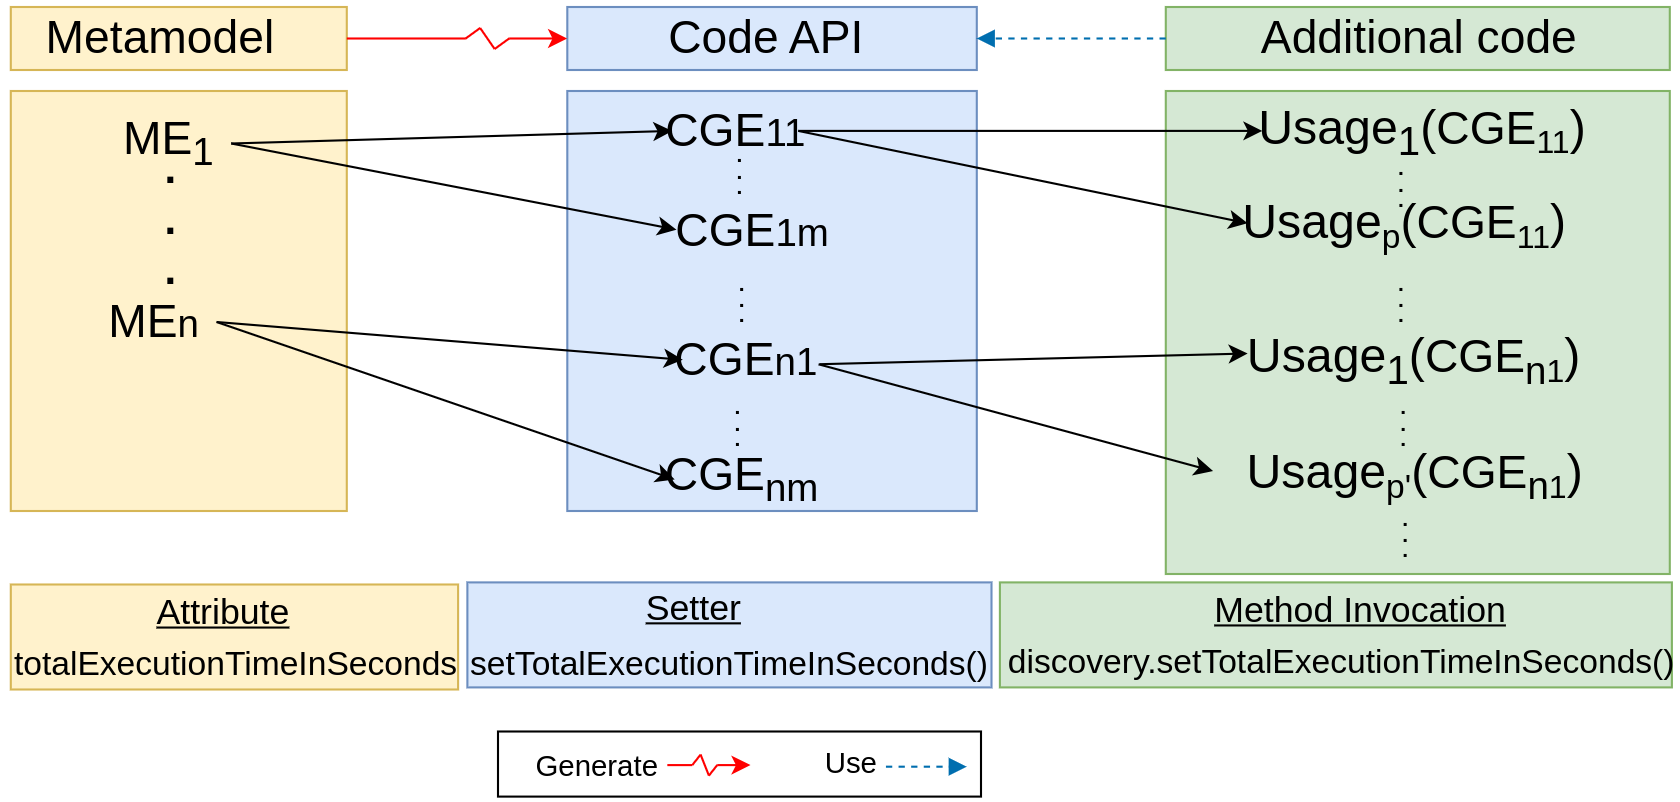
\includegraphics[width=0.5\textwidth]{pics/chapter1pics/patternusages.png}
	\caption{Schema for mapping between the metamodel and code.}
	\label{fig:patternconcept}
	\vspace{-1em}
	
\end{figure}

Algorithm \ref{algo :ErrorPatternalgo} summarizes the pattern matching process. 
Given a Java class, an error, and a list of metamodel changes, Algorithm~\ref{algo :ErrorPatternalgo} first retrieves the error AST node~{\small\boxed{line~2}}. After that, it identifies the configuration of the $GCE$ usages~{\small\boxed{Line~3}}. Then, for each metamodel change type ~{\small\boxed{lines~6,17,22,31}}, it identifies the pattern of the corresponding $GCE$ presented in Table~\ref{table:locationofMMelemen}~{\small\boxed{line~7,18,23,32}}. %the different cases of usages in the additional code~{\small\boxed{Lines~3, 2}}, \eg \emph{SimpleName}, \emph{QualifiedName}, \emph{SingleVariable}, \emph{MethodDeclaration}, etc, which are AST node types depending on its level and its position in the AST of the Java class. 
%Then, it matches it with the metamodel change causing its error~{\small\boxed{Lines ~5, 15, 18}}. This process is applied for the rest of the metamodel changes. 
%When the algorithm finds the causing change, it starts to find the 
Depending on the detected configuration, the appropriate pre-selected resolution is added to the output set~{\small\boxed{Line~10,13,19,26,35}}.
Finally, the selected resolutions set is returned for further processing in the automatic co-evolution~{\small\boxed{Line~41}}. 
Let us take the example of \texttt{"Change property type from S to T"} (last change type in Table \ref{table:ResolutionsCatalog}). It has two possible resolutions, CR16 and CR17. Assuming that we have a code error that must be co-evolved. Our pattern matching process first identifies the pattern of the corresponding $GCE_i$ from Table~\ref{table:locationofMMelemen} (Line 7), then the configuration of the $GCE_i$ usage (Lines 8). 
Algorithm \ref{algo :ErrorPatternalgo} starts by parsing the error to find the pattern of the corresponding $GCE_i$, which will help to find the causing change. The next step is to define the configuration of the $GCE_i$ which means the type of the $GCE_i$ usage. 
If it is a variable declaration (line 9), the resolution $CR16$ is returned. If any other configuration is detected, the pattern matching process returns $CR17$ as an appropriate resolution.

Note that an error can be matched with more than one resolution because a metamodel element $ME$ can be impacted by more than one change, in other terms interdependent changes. 
For example, \red{Algorithm~\ref{algo :ErrorPatternalgo} allows matching the error in~{\small\boxed{Line 17}} (rename property) and ~{\small\boxed{Line 31}} (move property) with two metamodel changes of the property \emph{totalExecutionTimeInSeconds} in Listing~\ref{lis:Modisco_Code_External_V1}.} The generated literal, which is our generated code element $GCE_i$, is used here in the configuration of a literal static field access 
\emph{\footnotesize{BenchmarkPackage.DISCOVERY\_\_TOTAL\_EXECUTION\_TIME\_IN\_SECONDS}}. The returned resolutions are $CR5$ and $CR10$~{\small\boxed{Line 19,35}}, \red{to be executed in the order of detection of their causing metamodel changes.}%\red{Empirically, we observe only the case of interdependency between a rename and move/pull/push changes.}

%Note that several patterns can be matched for a given error caused by multiple changes.
%For example, in Listing~\ref{lis:Modisco_Code_External_V1}, Algorithm~\ref{algo :ErrorPatternalgo} allows to match the error in~{\small\boxed{line 6}} with two patterns caused by the two metamodel changes rename and move of the property \emph{totalExecutionTimeInSeconds}. The generated literal, which is our generated code element $GCE_i$, used here in a static field access, 
%\emph{\footnotesize{BenchmarkPackage.DISCOVERY\_\_TOTAL\_EXECUTION\_TIME\_IN\_SECONDS}}. The matched patterns are \texttt{RenameProperty\_Literal} and \texttt{MoveProperty\_Literal}. %\texttt{RenameProperty\_ SimpleName\_Literal} and \texttt{MoveProperty\_SimpleName\_Literal}. 
%In total, we define 33 patterns that we match with the code usages and metamodel changes. We attach their list as a supplementary material\footnote{\url{https://figshare.com/s/8986914e924300be77da}}.
%Due to lack of space we attach their list as a supplementary material.



A similar mechanism is implemented for the rest of metamodel changes to select a resolution based on the pattern of $GCE_i$ and the configuration of its usage. % ~{\small\boxed{Lines 40-42}}.
For the sake of readability, Algorithm \ref{algo :ErrorPatternalgo} does not show all possible combinations of $metamodel$ $changes \times patterns \times configurations$, but few examples to illustrate its essence. \red{We nonetheless give an extended version in the appendix}

%
Finally, in our implementation, for the case of a "Delete Class" and "Delete Property", we favor the least deletion when possible. In particular, depending on the configuration usage, we select the resolution that deletes the least possible among $CR1$, $CR2$, $CR3$, $CR4$. For example, for an error in a parameter of a method call, we select the resolution $CR4$ rather than $CR1$ or $CR2$. 
In Listing \ref{lis:Modisco_Code_External_V1}, Algorithm \ref{algo :ErrorPatternalgo} matches the error in the import declaration (\textbf{Configuration}), with the deletion of the metaclass \textit{ProjectDiscovery} (\textbf{pattern}), which allows to select the resolution $CR2$.

%However, this is an implementaion strategy and could  

%For example, in Listing \ref{lis:Modisco_Code_External_V1}, the marker in {\small\boxed{line 6}}  \ie
%\texttt{BenchmarkPackage.} \emph{DISCOVERY\_\_TOTAL\_EXECUTION\_TIME\_IN\_SECONDS}  which is a static field access presents an erroneous usage of the $GCE_i$  Literal of an attribute caused by the metamodel change rename the property \emph{totalExecutionTimeInSeconds} to \emph{discoveryTimeInSeconds}. Algorithm \ref{algo :ErrorPatternalgo} allows to match it  with the pattern RenameProperty\_SimpleName\_Literal.


\definecolor{circlegreen}{HTML}{7ed321}



\begin{algorithm2e}[t]
	% \algsetup{linenosize=\tiny}
	\small
	
	\SetAlgoLined
	\KwData{javaClass, error, changesList}
	
	resolution\_s $\leftarrow \phi$ 
	
	%\While{(!usage.hasPatterns())}
	%{
		errorNode $\leftarrow$ findErrorAstNode(javaClass, error)
		
		configuration $\leftarrow$ getConfiguration(javaClass,errornode)
		
		%change $\leftarrow$ changesList.next()
		
		\For {(change  $\in$ changesList)}
		{
			\Switch{change}{
				\Case{ChangePropertyType}{
					\uIf{(match(patternGCE,change)}
					{
						
						\Switch{configuration}{
							
							\Case{VariableDeclaration}{
								
								resolution\_s.add("CR16")
							}
							
							\Other{
								
								resolution\_s.add("CR17")
							}
							
							
							
						}
					}
					
					
				}
				
				\Case{RenameProperty}{
					\uIf{(match(patternGCE,change)}
					{
						%configuration $\leftarrow$ getConfiguration(javaClass,errornode)
						
						resolution\_s.add("CR5")
						
					}
					
				}
				
				
				\Case{DeleteClass}{
					\uIf{(match(patternGCE,change)}
					{
						
						\Switch{configuration}{
							
							\Case{ImportDeclaration}{
								
								resolution\_s.add("CR2")
							}
							
							...  \emph{\textcolor{circlegreen}{/*Other configurations*/}}
							
						}
					}
				}
				
				\Case{MoveProperty}{
					\uIf{(match(patternGCE,change)}
					{
						
						\Switch{configuration}{
							
							\Case{LiteralStaticField}{
								
								resolution\_s.add("CR10")
							}
							...  \emph{\textcolor{circlegreen}{/*Other configurations*/}}    
						}
					}
					
					
				}
				\Case{... \emph{\textcolor{circlegreen}{/*Other changes*/}} }{ ... } 
				
			} 
			
			
		}
		\textbf{return} resolution\_s
		
		
		\caption{Pattern matching algorithm}
		\label{algo :ErrorPatternalgo}
	\end{algorithm2e}
	
	
	%\subsubsection{Mapping of the metamodel generated code}
	
	%\begin{comment}
	%-inputs : changes, error node
	%- analysing structure : syntactical and position in the ast refering to the different usages of metamodel element.
	%-Example
	%\end{comment}
	
	
	%\subsubsection{Pattern Detection} 
	
	%\kaouter{add concrete example using a listing : OK}
	%\DK{here take first the time to explain the table 1 of the mapping between ME types and GCE types : OK}
	%In order to add more functionalities developers enrich the generated code.  During the development process of the additional functionalities, a developer may use these generated code elements \{ $GCE_0$, $GCE_1$, ..., $GCE_n$ \}. When the developper uses a  $GCE_i$, s/he can use it in different ways, for example, an attribute literal (Table \ref{table:locationofMMelemen} ) can be used as a method declaration and method invocation parameter, and/or  as a part of a variable declaration initializer.
	%If $ME$ is changed, all the usages of  $GCE_i$ will be impacted
	%\kaouter{ Remove general example : For example if we move an attribute from a class \textit {A} to another class \textit{B} through a reference, all  the \textbf{usages} of the corresponding elements shown in the table \ref{table:locationofMMelemen} will be impacted.}
	%For example, in Listing \ref{lis:Modisco_Code_External_V1}, {\small\boxed{line 6}}, the metamodel element $ME$ that has been changed is the attribute \textit{dicoveryDate} in the class \textit{Discovery}. The corresponding generated code element $GCE$ which  is an attribute literal ( table \ref{table:locationofMMelemen}) is used as Return statement.
	
	%Two changes has been applied on this $ME$ :
	
	
	\begin{comment}[noitemsep,nolistsep]
		\item RenameProperty: dicoveryDate to discoveryDate.
		\item MoveProperty: from the class \textit{Discovery } to the class \textit{DiscoveryIteration}.
	\end{comment}
	
	%Then the usage at { \small\boxed{line 6}} is marked as an error.
	%To be able to correct a defected usage of a $GCE_i$ catched as an error, we have to find a link between the marker and the changes that caused it. The pattern matching process analyses the AST node corresponding to the marker. It finds first its AST level ( SimpleName, QualifiedName,SingleVariable, MethodDeclaration ...etc) that depends on the particular usage of the $GCE_i$. Then it analyses syntactically the AST node to link it to the right changes.
	%The second step in pattern matching is to assign a pattern to the marker. We create a data structure called \textit{Usage} that includes: The error marker, the error node, the corresponding change, and different patterns that can be associated to the error marker.
	
	%For the previous example, two patterns are detected: \textit{LiteralRename} and \textit{LiteralMove}.
	
	
	%\kaouter{here of after say that => Direct and indirect errors : \\ direct error:  the node has syntactic relation with the change element or structure relation with it,( vd in method invocation ?}
	
	%\DK{what do you mean by the "the syntactic structure of the AST node of the error and its level in the AST" ? Also, try first to explain why you need a pattern matching strategy ? like due to the variety of GCE and where they are in the code, a different  pattern of resolution can be applied ? also do you distinguish pattern and resolution or are they mixed ? : OK}
	
	
	
	\begin{comment}
		
		For example, in  marker \ref{fig:java_marker}, the detected error is about the method \textit{\texttt{setName}}, because we renamed the attribute \textit{\texttt{name}} in the class \textit{\texttt{Person}}, into \te%\\
		xtit{\texttt{familyName}}. The detected error has a \textit{\texttt{SimpleName}} corresponding node. By analyzing the structure of the node, we find that the detected pattern is \textit{\texttt{setObjectRename}}.
		
	\end{comment}
	
	
	
	
	
	
	
	\begin{comment}
		
		
		\begin{algorithm2e}[t]
			% \algsetup{linenosize=\tiny}
			\small
			
			\SetAlgoLined
			\KwData{javaClass, error, changesList}
			
			usage $\leftarrow \phi$ 
			
			%\While{(!usage.hasPatterns())}
			%{
				errorNode $\leftarrow$ findErrorAstNode(javaClass, error)
				
				%change $\leftarrow$ changesList.next()
				
				
				\uIf{(errornode.isTypeOf( SimpleName))}
				{
					\For {(change  $\in$ changesList)}
					{
						\Switch{change}{
							\Case{MoveProperty}{
								\uIf{(errornode.name="get"+change.name V errornode.name="set"+change.name)}
								{
									usage.getPatterns().
									add(UsagePattern.MoveProperty\_GetSet)
								}
								\uElseIf{(errornode.name= 
									change.className +"\_\_" +change.name)}
								{
									usage.getPatterns().
									add(UsagePattern.MoveProperty\_Literal)
								}
								\uElseIf{(errornode.name= 
									change.className +"get" +change.name)}
								{
									\uIf{(change.getUpperBound= -1)}
									{
										usage.getPatterns().
										add(UsagePattern.MoveProperty\_UpperBoundMultiple)
									}
									
									
									\uElse{
										usage.getPatterns().
										add(UsagePattern.MoveProperty\_UpperBoundSingle)
										
									}
								}
								\uElseIf{(...)}
								{
									...
								}
								
							}
							\Case{RenameProperty}{
								...
							}
							\Case{DeleteProperty}{
								...
							}
						}
					}
				} \uElseIf {( errornode.isTypeOf( QualifiedName))}
				{	  \emph{\textcolor{circlegreen}{/*repeat same matching process*/}}
					...
				}
				
				%}
			\textbf{return} usage
			
			
			\caption{Pattern matching algorithm}
			\label{algo :ErrorPatternalgo}
		\end{algorithm2e}
		
		
		\begin{table*}[t]
			\begin{tabular}{|l|l|}
				\hline
				Inputs & \begin{tabular}[c]{@{}l@{}}1) Change: move property p from class A to class B through a reference ref\\ 2) AST level : Simple Name\\ 3) Syntactic link: The identifier of the Simple Name is "get+ The name of the moved property"  \\ or  "set + The name of the moved property"\end{tabular} \\ \hline
				Output & GetorSetMoveProperty pattern                                                                                                                                                                                                                                                               \\ \hline
			\end{tabular}
			\caption{Example of GetorSetMoveProperty pattern } 
			\label{table: GetorSetMovePropertyPattern}
		\end{table*}
		
	\end{comment}
	
	\begin{algorithm2e}[t]
		% \algsetup{linenosize=\tiny}
		\small
		\SetAlgoLined
		\KwData{EcoreModelingProject, changesList}
		javaClasses $\leftarrow$ Parse(EcoreModelingProject)
		
		\For {( jc $\in$ javaClasses)}
		{
			errorsList $\leftarrow $ getErrors(jc)
			
			\While{(!errorsList.isEmpty())}
			{
				error  $\leftarrow$ errorsList.next()
				
				resolution\_s $\leftarrow$ patternMatching(jc,error, changesList)
				
				\uIf{(! resolution\_s.isEmpty()) \emph{\textcolor{circlegreen}{/*direct errors*/}}}
				{
					\For {(resolution  $\in$ resolution\_s)}
					{
						applyResolution(jc,error, resolution)
					}
				}
				\uElseIf {error.hasQuickFix() \emph{\textcolor{circlegreen}{/*indirect errors*/}}}
				%{(is\_The\_Type\_Must\_Implement\_The\_Inherited\_Abstract\_Method)}
				{
					useQuickFixes(error) %\COMMENT{Eclipse quick fix}
				}
				%\uElse {break;}
				
				refreshJavaClass(jc) 
				
				refreshErrorsList(jc, errorsList)
			}
			
		}
		
		\caption{Co-evolution of metamodel and code}
		\label{algo :overallalgo}
	\end{algorithm2e}
	
	
	
	\begin{comment}
		
		\begin{algorithm2e}[t]
			% \algsetup{linenosize=\tiny}
			\small
			\SetAlgoLined
			\KwData{EcoreModelingProject, changesList}
			javaClasses $\leftarrow$ Parse(EcoreModelingProject)
			
			\For {( jc $\in$ javaClasses)}
			{
				errorsList $\leftarrow $ getErrors(jc)
				
				\While{(!errorsList.isEmpty())}
				{
					error  $\leftarrow$ errorsList.next()
					
					usage  $\leftarrow$ matchUsagePattern(jc, error, changesList)
					
					\uIf{(! usage.getPatterns().isEmpty()) \emph{\textcolor{circlegreen}{/*direct errors*/}}}
					{
						\For {(pattern  $\in$ usage.getPatterns())}
						{
							resolution $\leftarrow$ selectResolution(pattern)
							
							applyResolution(jc, usage.getErrorNode(), resolution)
						}
					}
					\uElseIf {error.hasQuickickFix() \emph{\textcolor{circlegreen}{/*indirect errors*/}}}
					%{(is\_The\_Type\_Must\_Implement\_The\_Inherited\_Abstract\_Method)}
					{
						useQuickFixes(error) %\COMMENT{Eclipse quick fix}
					}
					%\uElse {break;}
					
					refreshJavaClass(jc) 
					
					refreshErrorsList(jc, errorsList)
				}
				
			}
			
			\caption{Co-evolution of metamodel and code}
			\label{algo :overallalgo}
		\end{algorithm2e}
		
		
		
	\end{comment}
	
	
	
	
	\subsection{Repair mechanism for the code co-evolution}
	\label{repairmechanism}
	
	
	
	After the pattern matching step, we can proceed to co-evolve the code. 
	Herein, we distinguish \textbf{direct errors} and \textbf{indirect errors}. The former are errors that do use a Generated Code Element $GCE$. They can be matched with one or many metamodel changes to select the appropriate one or many resolution(s). 
	The latter are errors that %are caused also by the metamodel evolution but they 
	do not use a generated code element. They are not matched, and hence, cannot be resolved using the pattern matching process. %They are typically errors that appear after co-evolving the direct code errors.
	
	
	
	Algorithm \ref{algo :overallalgo} presents the general process of the code co-evolution. It starts by parsing the project Java classes {\small\boxed{line~1}} to be able to access the AST of the code. Then it browses the parsed classes to retrieve the list of errors {\small\boxed{line~3}}. 
	The next step is to run the pattern matching Algorithm \ref{algo :ErrorPatternalgo} for each error to return the matched resolution(s) if any {\small\boxed{lines~4-15}}. 
	%\todo{how to avoid infinite loop?}
	%In principle, applying the resolutions require the code AST and the matched usage patterns as input to produce the co-evolved AST as output, as depicted in Figure \ref{fig:schema_resolution}.
	% of the first erroneous code usage of an evolved metamodel element. 
	%Algorithm \ref{algo :ErrorPatternalgo} first retrieves the error AST node {\small\boxed{line 5}}. Then, it matches it with the metamodel change causing its error {\small\boxed{lines 5-19}}. In particular, it covers all different code usages of the metamodel elements that are presented in Table \ref{table:locationofMMelemen}.
	%
	%\red{//explain algo 2 quickly}
	%
	%build? the first defective \textbf{usage} that we can correct {\small\boxed{line 5}}. In algorithm \ref{algo :ErrorPatternalgo}, we try to classify each marker and to detect at least one pattern for this marker. To analyse the marker, we start by retrieving the correspondant AST node { \small\boxed{line 1}}. Then depending on the type of the \textbf{ AST node} ( its level in the AST)  { \small\boxed{lines 2, 9}} and the type of the \textbf{change}  { \small\boxed{line 4}}, we can access their properties to test if there is any relation between them. In case a relation is established, a corresponding pattern is assigned  { \small\boxed{line 6}}. The usage will contain the marker, the corresponding AST node, the change, and the found patterns. 
	%
	If an error is matched with at least one resolution {\small\boxed{line~7}}, it is a \textbf{direct error}. If an error is matched with several changes {\small\boxed{lines~8-10}}, it will be resolved iteratively for each resolution{\small\boxed{lines~9}}. 
	
	In the case of an \textbf{indirect error}, we cannot apply the pattern matching process, but we still attempt to repair them with the available quick fixes in the IDE. 
	%
	%For example, \emph{unimplemented method m() of the class C} which is considered as an indirect error.\red{ It can not be matched with a metamodel pattern, because the declaration of the class C is not a code usage of the method m() (Table \ref{table:locationofMMelemen}.}, we attempt to repair it with its quick fix \emph{add the unimplemented method}.%preselected quick fix
	%
	We analyze the error message to match it with one of the proposed Java quick fixes~{\small\boxed{lines~11}}. For example, \emph{the type MC must implement the inherited abstract method} is considered as an indirect error. 
	\blue{This error can occur when a method is added in a metaclass \texttt{MC}. Classes that implement the generated interface generated from \texttt{MC} must override the new method.}
	%OLD PULL \red{This error occurs when an attribute is pulled from  a metaclass A to another metaclass B. Classes that implemented the generated interface from B must override the new methods.} 
	%\red{ It can not be matched with a metamodel pattern, because the declaration of the class C is not a code usage of the method m() (Table \ref{table:locationofMMelemen})}, w
	We attempt to repair it with its quick fix \emph{add the unimplemented method}~{\small\boxed{lines~12}}.
	
	After applying the resolutions or a quick fix, the Java class has to be refreshed. This is because the modifications of the AST will impact the list of errors and their locations in the Java class {\small\boxed{lines~13-14}}. When 
	refreshing the Java class, the list of errors typically decreases as they are co-evolved,  
	%updating the list of errors, they decrease as we co-evolve them, 
	yet, new ones may be introduced. Consequently, they will be handled in the next iterations similarly with our pattern matching and co-evolution algorithm or with the quick fixes.
	
	Finally, this process is repeated until all errors are handled. 
	However, we implemented a stopping criteria to handle the indirect errors with quick fixes. 
	It stops in two cases: 1) when only errors without any quick fix proposal remain, or 2) when the application of a quick fix causes an infinite loop \cite{cuadrado2018quick,khelladi2019detecting}, i.e., a cycle of applying a quick fix that causes a previously fixed error (A $\mapsto$ B $\mapsto$ A $\mapsto$ B $\mapsto$ ...). However, as we will see in the evaluation, these cases never happened in our executions. 
	
	%The stop condition is guaranteed because all the errors are due to metamodel changes and once an error is detected, it can be resolved using pattern matching or quick fixes.
	%\todo{say there is a risk of infinite loop between qucik fixes, and that we haev stoping cirteria for it.}  
	%Otherwise, only errors that are not matched with pattern usages and can't be resolved with quick fixes remain.
	%.all we find a defected usage that we don't know how to correct.
	
	Note that during the co-evolution process, we log the history of execution: the Java class, the error, its line, the change that provoked it, and the applied resolution(s)/quick fix in a generated report. Thus, we can generate a detailed report that allows the developer to check the modifications applied to the co-evolved code after the co-evolution is finished, i.e, their validation is not mendatory to concretly apply the resolutions.
	Table \ref{table:report} shows an example of a report for the corresponding part to our motivation example from Modisco Java Discoverer Benchmark applied co-evolution. %\red{maybe put it in 3.6?}
	
	%\red{//TODO add table of resolutions}
	
	
	%%%%%%%%%%%%%%%%%%%%%%%%%%%%%%%%%%%%%%%%%%%%%%%%%%%%%%%%%%%%%%%%%%%%%%%%%
	
	
	
	\begin{table*}[t]
		%\begin{wraptable*}{r}{5.5cm}
		\centering
		\caption{Excerpt from the traced report of Modisco Java Discoverer Benchmark project}
		\label{table:report}
		%
		%\small
		%\hspace*{-2em}
		\resizebox{17cm}{!}{
			\begin{tabular}{
					@{\hskip3pt}c@{\hskip3pt}|c@{\hskip3pt}|c@{\hskip3pt}|c@{\hskip3pt}|c@{\hskip3pt}|c@{\hskip3pt}|c@{\hskip3pt}|c@{\hskip3pt}}
				\toprule 
				File & Error& Line &Change & Resolution\\ \midrule
				\begin{tabular}[c]{@{}l@{}}CDOProjectDiscoveryImpl.java\end{tabular}
				& \begin{tabular}[c]{@{}l@{}} ProjectDiscovery \end{tabular} 
				& \begin{tabular}[c]{@{}l@{}}  29  \end{tabular} 
				&\begin{tabular}[c]{@{}l@{}}  Delete class \\ProjectDiscovery  \end{tabular}  
				&\begin{tabular}[c]{@{}l@{}}  CR2 \end{tabular}  
				
				\\ \midrule
				
				
				\begin{tabular}[c]{@{}l@{}}Report.java\end{tabular} 
				& \begin{tabular}[c]{@{}l@{}} setTotalExecutionTimeInSeconds \end{tabular}
				& \begin{tabular}[c]{@{}l@{}}  183  \end{tabular} 
				&\begin{tabular}[c]{@{}l@{}}  Rename property   \end{tabular}  
				&\begin{tabular}[c]{@{}l@{}}  CR5 \end{tabular}  
				
				\\ \midrule
				\begin{tabular}[c]{@{}l@{}}Report.java\end{tabular} 
				& \begin{tabular}[c]{@{}l@{}} setDiscoveryTimeInSeconds \end{tabular}
				& \begin{tabular}[c]{@{}l@{}}  183  \end{tabular} 
				&\begin{tabular}[c]{@{}l@{}}  Moving property  \end{tabular}  
				&\begin{tabular}[c]{@{}l@{}}  CR7  \end{tabular}  
				
				\\ \midrule
				
				\begin{tabular}[c]{@{}l@{}}CDOProjectDiscoveryImpl.java\end{tabular}
				& \begin{tabular}[c]{@{}l@{}} DISCOVERY\_\_TOTAL\_EXECUTION\_TIME\_IN\_SECONDS \end{tabular}
				& \begin{tabular}[c]{@{}l@{}}  799\end{tabular}
				&\begin{tabular}[c]{@{}l@{}}  Rename property  \end{tabular}   
				&\begin{tabular}[c]{@{}l@{}}  CR5  \end{tabular}  
				\\ \midrule
				\begin{tabular}[c]{@{}l@{}}CDOProjectDiscoveryImpl.java\end{tabular}
				& \begin{tabular}[c]{@{}l@{}} DISCOVERY\_\_DISCOVERY\_TIME\_IN\_SECONDS \end{tabular}
				& \begin{tabular}[c]{@{}l@{}}  799\end{tabular}
				&\begin{tabular}[c]{@{}l@{}}  Move property \end{tabular}   
				&\begin{tabular}[c]{@{}l@{}}  CR10\end{tabular}  
				
				\\ 
				
				
				\bottomrule
			\end{tabular}
		}
		%\end{wraptable*} 
		\vspace{-1em}
	\end{table*}
	
	%%%%%%%%%%%%%%%%%%%%%%%%%%%%%%%%%%%%%%%%%%%%%%%%%%%%%%%%%%%%%%%%%%%%%
	\begin{comment}
		
		\begin{table}[t!]
			\caption{ Patterns of usage and their corresponding resolutions.}
			\label{listofpatterns}
			\resizebox{8cm}{!} {
				\begin{tabular}{ll}
					\toprule
					Pattern of usage     & Associated resolution	 \\ \midrule		
					RenameProperty_SimpleName & CR5  \\ \midrule		
					RenameProperty_Get     & CR5  \\ \midrule		
					RenameProperty_Set    & CR5\\ \bottomrule	
					RenameProperty_Literal    & CR5\\ \bottomrule	
					RenameClass_TypeUse   & CR5\\ \bottomrule	
					RenameClass_SuperType    & CR5\\ \bottomrule	
					RenameClass_getObject    & CR5\\ \bottomrule	
					RenameClass_setObject    & CR5\\ \bottomrule	
					RenameClass_Import    & CR5\\ \bottomrule	
					RenameClass_ImportImpl    & CR5\\ \bottomrule	
					RenameClass_QualifiedType   & CR5\\ \bottomrule	
					DeleteClass_VariableDeclaration   & CR2\\ \bottomrule	
					DeleteClass_parameter    & CR1\\ \bottomrule	
					DeleteClass_parameterInMi    & CR1\\ \bottomrule	
					DeleteClass_Import    & CR2\\ \bottomrule	
					DeleteClass_MethodInvocType    & CR1\\ \bottomrule	
					DeleteClass_ClassInstance   & CR2\\ \bottomrule	
					DeleteClass_ReturnType    & CR1\\ \bottomrule	
					DeleteClass_SuperClass   & CR1\\ \bottomrule	
					DeleteClassProperty_Literal & CR4\\ \bottomrule	
					DeleteClass_ComplexStatement   & CR2\\ \bottomrule	
					DeleteClass_GetObject   & CR1\\ \bottomrule	
					DeleteProperty_MethodInvocation  & CR3\\ \bottomrule	
					MoveProperty_GetSet   &  \begin{tabular}[c]{@{}l@{}} CR7 and CR8 \\( depending on the upperBound of ref)\end{tabular}\\ \bottomrule	
					MoveProperty_MethodInvocation   & \begin{tabular}[c]{@{}l@{}} CR7 and CR8 \\( depending on the upperBound of ref)\end{tabular}   \\ \bottomrule	
					MoveProperty_MethodDeclaration  & \begin{tabular}[c]{@{}l@{}} CR7 and CR8 \\( depending on the upperBound of ref)\end{tabular}\\ \bottomrule	
					MoveProperty_Literal  & CR10\\ \bottomrule	
					PushProperty_Literal  & CR13\\ \bottomrule	
					PushProperty_GetSet  & CR11\\ \bottomrule	
					PullProperty_Literal  & CR14\\ \bottomrule	
					GeneralizeProperty_MethodInvocation   & CR6\\ \bottomrule	
					ChangeType_MethodInvocation  & CR16\\ \bottomrule	
					
				\end{tabular}
			}
		\end{table}
		%\vfill
	\end{comment}
	
	
	
	\begin{comment}
		
		\begin{algorithm}[t]
			\algsetup{linenosize=\tiny}
			\small
			\SetAlgoLined
			\KwData{cu, markersList, changesList}
			
			\For {<marker $\in$ markersList> }
			{
				usage $\leftarrow$ classify(cu,marker,changes)
				
				\uIf{(! usage.gePatterns().isEmpty())}
				{
					output $\leftarrow$  usage;
				}
			}
			output $\leftarrow$ null 
			\caption{Get first non-null usage algorithm}
			\label{algo :Usagealgo}
		\end{algorithm}
		
		
		
	\end{comment}
	
	
	
	
	
	
	
	%\subsection{Testing co-evolution}
	
	%Note that our pre-selection of a resolution may lead to a doubt about the behavioral correctness of the coevolved code. This is why we opted for the use of unit tests before and after the coevolution to check the code behavioral correctness. \todo{maybe say it in the end of 3.6 repair section, also this is part of the eval and not teh appproch, so better say it in the eval process (i think we do already)}
	
	\subsection{Prototype Implementation}
	%To be able to evaluate our approach, 
	We implemented our solution as an Eclipse Java plugin handling Ecore/EMF metamodels and their Java code. 
	
	%\red{The change detection uses EMFCompare library to compare two Ecore metamodels, the result is then formatted in our change detection interface}.
	The co-evolution process technically consists of the code AST manipulation using the JDT eclipse plugin\footnote{Eclipse Java development tools (JDT): \url{https://www.eclipse.org/jdt/core/}}.
	\begin{itemize}
		\item \textbf{Error retrieving}: there are many methods to manipulate the compilation errors of the code. We use the marker of IJavaModelMarker.JAVA\_MODEL\_PROBLEM\_MARKER. Then we filter markers whose severity value equals 2.
		\item \textbf{Change detection layer}: it consists of a set of model classes that specifies the information of each type of atomic and complex changes. 
		\item \textbf{Pattern matching}: to match the error AST node with the causing change, we proceed by string formatting between the identifier of the AST node and the relevant information encapsulated in the change. We find the corresponding configuration by looking for the higher levels of the error AST node in the code AST using the package org.eclipse.jdt.core.dom.
		\item \textbf{Resolutions} :
		The AST nodes of errors are manipulated with edit actions: modification, replacement, or deletion)  
		using the package \textit{ org.eclipse.jdt.core.dom.rewrite}, org.eclipse.text.edits.TextEdit, and \textit{org.eclipse.core.filebuffers}. 
		\item \textbf{Quick fixes} : we use \textit{org.eclipse.jdt.ui.text.java.IQuickAssistProcessor} and \textit{org.eclipse.jdt.ui.text.java.IJavaCompletionProposal}.
		
	\end{itemize}
	%To facilitate the use of our tool, we added a command the xml file of the pluginsloppypar. 
	
	%The developer replaces the old version of the metamodel with the new one, and then regenerates the code API. After the regeneration step, errors will be provoked in the developer's code. He starts by selecting the path of the old and new versions of the metamodel, then he right-clicks his project, and he chooses "Coevolve the code" to run our approach. At the end of the execution, his project is coevolved and a report with the history of the execution can be found in the project's folder.
	The source code of the prototype can be found by following this link \footnote{\url{https://figshare.com/s/8986914e924300be77da}}.
	%In section \ref{repairmechanism}, we mentioned that after each resolution, we need to update the list of errors, for that, we need to save the AST after each modification  using package  \textit{org.eclipse.core.filebuffers}.
	%\red{Supplementary materials are provided\footnote{companion web page}}
	%For the metamodel changes we use an existing approach \cite{Alter2015, williams2012searching,cicchetti_managing_2009,langer_posteriori_2013,vermolen_reconstructing_2012,Khelladi2016}. 
	
	%\todo{here say that we generate a report linking mm changes, to impacted lines in the code, error message, matched pattern, and how they were co-evoved it which resoluton}
	
	\section{Evaluation}\label{eval}
	
	This section evaluates our automatic co-evolution approach. 
	First, we present the evaluation process and the data set. Then, we set the research questions we address and discuss the obtained results.
	
	
	\subsection{Evaluation Process}
	
	We evaluate our automated co-evolution of code with metamodel evolution by measuring: 1) its ability to co-evolve the errors, 2) its time performance, 3) its correctness by using recall and precision metrics, 4) its behavioral correctness by using test suites before/after the automatic co-evolution, 5) and by comparing it with both quick fixes and our prior work~\cite{Khelladi2020}. %programmatically applying quick fixes.}
	%% checking changes mentionned in threats to validity 
	%%Before starting the evaluation process, we confirm the changes of %%metamodel. As these changes from version \emph{1} to version~\emph{2} serve %%as input of our automatic code co-evolution
	
	First, as our approach co-evolves the erroneous code due to metamodel evolution, we need to \textbf{provoke the errors in the code}. To do so, we replace the original metamodel with the evolved metamodel. Then, we regenerate the code API with EMF. This will cause errors in the code that our approach must co-evolve~(1).  
	We then use the function $System.nanoTime()$ for time measurement~(2). 
	After that, we measure the correctness of our code co-evolution~(3) by comparing, for the same set of code errors that we automatically co-evolved, how they were manually co-evolved by developers. This allows us to measure the \emph{precision} and \emph{recall} reached by our co-evolution approach. They vary from~0 to~1, i.e., 0\% to 100\%. They are defined as follows:
	%We evaluate correctness by measuring \emph{precision} and \emph{recall}. We compare our applied co-evolution with the manually applied co-evolved by developers against our proposed co-evolution. 
	%
	%This allows us to measure the correctness of our co-evolution approach. %, i.e., correctness  of our proposed co-evolution. 
	%
	%In this experiment, we measure the correctness of our approach by using the two metrics \emph{precision} and \emph{recall} that 
	%\emph{Precision} and \emph{recall} vary from 0 to 1, i.e., 0\% to 100\%. They are defined as follows:
	%three case studies from three different language implementations in Eclipse, namely OCL \cite{MDTOCL}, Modisco \cite{MDTModisco}, and Papyrus \cite{MDTPapyrus}. 
	%The correctness metric of our automated co-evolution is computed as follows:
	
	%\vspace{0.8em}
	%$ correctness = \dfrac{Applied Resolutions \cap Expected Resolutions}{Applied Resolutions} $
	%\vspace{0.8em}
	
	%The $Applied Resolutions$ are the resolutions applied by our approach (from Table \ref{table:ResolutionsCatalog}) and  the $Expected Resolutions$ are the actual manually performed resolutions by developers. The correctness varies from 0 to 1, i.e., 0\% to 100\%. %\red{Note that}
	
	\vspace{1em}
	\noindent $ precision = \dfrac{Applied Resolutions \cap Expected Resolutions}{Applied Resolutions} $
	
	\vspace{1em}
	
	\noindent $ recall = \dfrac{Applied Resolutions \cap Expected Resolutions}{Expected Resolutions} $
	\vspace{1em}
	
	The $Applied Resolutions$ are those by our approach (from Table \ref{table:ResolutionsCatalog}) and  the $Expected Resolutions$ are the actual manually performed resolutions by developers.  %The precision and recall  %The higher the precision value, the smaller is the set of wrong resolutions that have been proposed (i.e. false positives). The higher the recall value, the smaller is the set of the expected resolutions that have not been proposed (i.e. false negatives).
	
	Moreover, to check if the co-evolution impacts the original code behavior~(4), we generate tests for the original and the automatically co-evolved versions. Hence, we observe the behavioral effect of our co-evolution through the tests. To do so, we rely on Evosuite~\cite{fraser2011evosuite}, a popular tool for test cases generation, as it is widely used by researchers and developers. 
	Gruber et al. \cite{gruber2023automatic} further showed the quality and robustness of the generated tests. It showed that while flakiness is at least as common in generated tests as in developer-written tests, EvoSuite is effective in alleviating this issue giving 71.7\% fewer flaky tests. Thus, EvoSuite is appropriate in our work to generate robust tests in the original code and in the co-evolved code to compare their results, i.e., check behavioral correctness.
	
	Furthermore, we compare our approach with the application of quick fixes~(5). For each error, we apply the first quick fix in the list of corresponding proposals, then we compare the precision and recall of quick fixes with the precision and recall of our approach.
	%
	Finally, we compare our approach with our prior work~\cite{Khelladi2020} in terms of precision and recall, and general rationale (5).
	%Note that we studied evolved and original versions to confirm the metamodel changes and code co-evolution from version \emph{1} to version~\emph{2}. 
	
	%Based on those changes we run an impact analysis to identify the impacted parts of the code that will be co-evolved. 
	
	
	
	%%%%%%%%%%%%%%%%%%%%%%%%%%%%%%%%%%%%%%%%%%%%%%%%%%%%%%%%%%%%%%%%%%%%%%%%%%%%%%%%%%%%%%%%%%%%%%%%%%%%%%%%%%%%%%%%%%%%%%%%%%%%%%%%%%%%%%%%%%%%%%%%%%%%%%%%%%%%%%%
	% Please add the following required packages to your document preamble:
	% \usepackage{multirow}
	
	\begin{table*}[t]
	\centering
	\caption{Details of the metamodels and their evolutions.}
	\label{CaseStudies_Evolution}
	\resizebox{16.2cm}{!} {
		\begin{tabular}{cllll}
			\toprule
			Case study                                                                            & \begin{tabular}[c]{@{}l@{}}Evolved \\ metamodels\end{tabular}                 & Versions & %\begin{tabular}[c]{@{}l@{}}Size ($N^{o}$ of\\ elements)\end{tabular} &
			\multicolumn{1}{c}{\begin{tabular}[c]{@{}c@{}}Atomic changes \\in the metamodel\end{tabular}} & \multicolumn{1}{c}{\begin{tabular}[c]{@{}c@{}}Complex changes \\in the metamodel\end{tabular}} \\ \midrule		
			
			%\multirow{6}{*}{\begin{tabular}[c]{@{}l@{}}OCL\end{tabular}} 
			OCL & \begin{tabular}[c]{@{}l@{}}Pivot.ecore in project\\ocl.examples.pivot\end{tabular}                        &  \begin{tabular}[c]{@{}l@{}}3.2.2 to\\ 3.4.4\end{tabular}        &   %\begin{tabular}[c]{@{}l@{}}Original: 1473 \\Evolved: 1787\end{tabular}  &
			\begin{tabular}[c]{@{}l@{}} Deletes: 2 classes, 16 properties, 6 super types \\ Renames: 1 class, 5 properties \\ Property changes: 4 types; 2 multiplicities \\ Adds: 25 classes, 121 properties, 36 super types  \end{tabular}                                                         &    \begin{tabular}[c]{@{}l@{}} 1 pull property \\ 2 push properties  \end{tabular}                                                        \\ \midrule %cmidrule{2-5} %midrule		
			
			%	& \begin{tabular}[c]{@{}l@{}}Base.ecore in project\\ocl.examples.xtext.base\end{tabular}                         &   \begin{tabular}[c]{@{}l@{}}3.1.0 to\\ 3.4.4\end{tabular}       &  %\begin{tabular}[c]{@{}l@{}}Original: 272 \\Evolved: 357\end{tabular}   &  	\begin{tabular}[c]{@{}l@{}} Deletes: 4 classes, 11 properties, 17 super types \\ Renames: 1 property \\ Property changes: 2 type \\ Adds: 10 classes, 38 properties, 19 super types \\ Total = 102 \end{tabular}                                                       &      \begin{tabular}[c]{@{}l@{}} 5 moves properties \\ 1 push property \\ 2 extract class \\ 2 extract super class\\ Total = 10 \end{tabular}                                                      \\ \midrule
			%		& \begin{tabular}[c]{@{}l@{}}OCL \\ "EssentialOCL"\end{tabular}                 &          &      &                                                           &                                                            \\ \midrule
			%		& \begin{tabular}[c]{@{}l@{}}OCL \\ "CompleteOCL"\end{tabular}                  &          &      &                                                           &                                                            \\ \midrule
			Modisco & \begin{tabular}[c]{@{}l@{}}Benchmark.ecore in project\\modisco.infra.discovery.benchmark\end{tabular}                & \begin{tabular}[c]{@{}l@{}}0.9.0 to\\ 0.13.0\end{tabular}         &   %\begin{tabular}[c]{@{}l@{}}Original: 95 \\Evolved: 106\end{tabular}    &  
			\begin{tabular}[c]{@{}l@{}} Deletes: 6 classes, 19 properties, 5 super types \\ Renames: 5 properties  \\ Adds: 7 classes, 24 properties, 4 super types  \end{tabular}                                                        &     \begin{tabular}[c]{@{}l@{}} 4 moves property \\ 6 pull property \\ 1 extract class \\ 1 extract super class \end{tabular}                                                       \\ \midrule		
			
			%\multirow{4}{*}{\begin{tabular}[c]{@{}l@{}}Papyrus\end{tabular}} 
			Papyrus & \begin{tabular}[c]{@{}l@{}}ExtendedTypes.ecore in project\\papyrus.infra.extendedtypes\end{tabular}            & \begin{tabular}[c]{@{}l@{}}0.9.0 to\\ 1.1.0\end{tabular}         & %\begin{tabular}[c]{@{}l@{}}Original: 40 \\Evolved: 57\end{tabular}     &   
			\begin{tabular}[c]{@{}l@{}}Deletes: 10 properties, 2 super types \\ Renames: 3 classes, 2 properties \\ Adds: 8 classes, 9 properties, 8 super types  \end{tabular}                                                      &    \begin{tabular}[c]{@{}l@{}} 2 pull property \\ 1 push property \\ 1 extract super class \end{tabular} \\  \bottomrule %\cmidrule{2-5} %midrule		
			
			%& \begin{tabular}[c]{@{}l@{}}Configuration.ecore in project \\ papyrus.infra.queries.core.configuration\end{tabular}            & \begin{tabular}[c]{@{}l@{}}0.9.0 to\\ 1.1.0\end{tabular}         & %\begin{tabular}[c]{@{}l@{}}Original: 24 \\Evolved: 0\end{tabular}     &     		\begin{tabular}[c]{@{}l@{}}Deletes: 6 classes, 7 properties, 4 super types \\ Total = 17 \end{tabular}                                                      &    \begin{tabular}[c]{@{}l@{}} none \end{tabular}	\\ \bottomrule                                         
		\end{tabular}
	}
	\end{table*}
	
	
	
	\begin{table*}[t]
	\caption{Details of the projects and their caused direct and indirect errors by the metamodels evolution.}
	\label{CaseStudies_CoEvolution}
	\resizebox{18cm}{!} {
		\begin{tabular}{llcccccc}
			\toprule
			\begin{tabular}[c]{@{}l@{}}Evolved \\ metamodels\end{tabular}                 & \begin{tabular}[c]{@{}l@{}}Projects to co-evolve in response to the \\ evolved metamodels \end{tabular} 	& \begin{tabular}[c]{@{}c@{}}$N^{o}$ of \\ packages\end{tabular} & \begin{tabular}[c]{@{}c@{}}$N^{o}$ of \\ classes\end{tabular} & %\begin{tabular}[c]{@{}c@{}}N° of \\ methods\end{tabular} & 
			\begin{tabular}[c]{@{}c@{}}$N^{o}$ of \\ LOC\end{tabular} & \begin{tabular}[c]{@{}c@{}}$N^{o}$ of Impacted \\ classes\end{tabular} & \begin{tabular}[c]{@{}c@{}}$N^{o}$ of total \\ direct errors \end{tabular}& \begin{tabular}[c]{@{}c@{}}$N^{o}$ of total \\ indirect errors \end{tabular}\\ \midrule		
			
			\begin{tabular}[c]{@{}l@{}}OCL \\ Pivot.ecore\end{tabular}                        & \begin{tabular}[c]{@{}l@{}}$[P1]$ ocl.examples.pivot\\ $[P2]$ ocl.examples.xtext.base\end{tabular}      &   \begin{tabular}[c]{@{}l@{}}22\\12 \end{tabular}     & \begin{tabular}[c]{@{}l@{}}439\\181 \end{tabular}                 &                                          %  \begin{tabular}[c]{@{}l@{}}5445\\1984 \end{tabular}              & 
			\begin{tabular}[c]{@{}l@{}}74002\\17599 \end{tabular} & \begin{tabular}[c]{@{}l@{}} 56\\10 \end{tabular} & \begin{tabular}[c]{@{}l@{}} 489\\27 \end{tabular} & \begin{tabular}[c]{@{}l@{}} 37\\2 \end{tabular} \\ \midrule		
			
			%		& \begin{tabular}[c]{@{}l@{}}OCL \\ "EssentialOCL"\end{tabular}                 & \begin{tabular}[c]{@{}l@{}}ocl.examples.xtext.essentialocl\\ ocl.examples.xtext.essentialocl.ui\\ ocl.examples.xtext.completeocl\\ ocl.examples.xtext.console\\ ocl.examples.xtext.oclinecore.ui\\ ocl.examples.xtext.oclinecore\\ ocl.examples.xtext.oclstdlib\end{tabular} &                                                      &                                                           &                                                          &                                                          \\ \midrule
			%		& \begin{tabular}[c]{@{}l@{}}OCL \\ "CompleteOCL"\end{tabular}                  & \begin{tabular}[c]{@{}l@{}}ocl.examples.xtext.completeocl\\ ocl.examples.xtext.completeocl.ui\end{tabular}                                                                                                                                                                   &                                                      &                                                           &                                                          &                                                          \\ \midrule
			\begin{tabular}[c]{@{}l@{}}Modisco \\ Benchmark.ecore\end{tabular}                & \begin{tabular}[c]{@{}l@{}} $[P3]$ modisco.infra.discovery.benchmark\\ $[P4]$ gmt.modisco.java.discoverer.benchmark\\ $[P5]$ modisco.java.discoverer.benchmark\\ $[P6]$ modisco.java.discoverer.benchmark.javaBenchmark\end{tabular}   & \begin{tabular}[c]{@{}l@{}}3 \\8 \\10 \\3  \end{tabular} & \begin{tabular}[c]{@{}l@{}}28 \\21 \\28 \\16 \end{tabular} & %\begin{tabular}[c]{@{}l@{}}\\ \\ \\  \end{tabular}  & 
			\begin{tabular}[c]{@{}l@{}}2333 \\1947 \\2794 \\1654 \end{tabular}  & \begin{tabular}[c]{@{}l@{}}1\\4 \\9 \\9 \end{tabular} & \begin{tabular}[c]{@{}l@{}}6 \\30 \\56 \\58 \end{tabular} & \begin{tabular}[c]{@{}l@{}}0 \\0 \\0 \\15 \end{tabular}  \\ \midrule		
			
			\begin{tabular}[c]{@{}l@{}}Papyrus \\ ExtendedTypes.ecore\end{tabular}            & \begin{tabular}[c]{@{}l@{}} $[P7]$ papyrus.infra.extendedtypes\\  $[P8]$ papyrus.infra.extendedtypes.emf\\  $[P9]$ papyrus.uml.tools.extendedtypes\end{tabular}  & \begin{tabular}[c]{@{}l@{}}8 \\7 \\7 \end{tabular} & \begin{tabular}[c]{@{}l@{}}37 \\12 \\15  \end{tabular} & %\begin{tabular}[c]{@{}l@{}}\\  \\  \end{tabular}  & 
			\begin{tabular}[c]{@{}l@{}}2057 \\374 \\725  \end{tabular}  & \begin{tabular}[c]{@{}l@{}}8 \\7  \\7 \end{tabular} & \begin{tabular}[c]{@{}l@{}} 59\\23\\23 \end{tabular} & \begin{tabular}[c]{@{}l@{}}0\\6 \\6\end{tabular} \\ \bottomrule		
		\end{tabular}
	}
	\end{table*}
	
	
	
	
	%%%%%%%%%%%%%%%%%%%%%%%%%%%%%%%%%%%%%%%%%%%%%%%%%%%%%%%%%%%%%%%%%%%%%%%%%
	
	%%%%%%%%%%%%%%%%%%%%%%%%%%%%%%%%%%%%%%%%%%%%%%%%%%%%%%%%%%%%%%%%%%%%%%%%%
	
	
	\subsection{Data Set}
	\begin{comment}
	
	
	\kaouter{The authors do not describe the used dataset, it is necessary to have a better understanding of how it represents real-world needs. OK}
	\kaouter{
		
		(MDE\_Eclipse): Moreover, Eclipse IDE in 2022 was downloaded 1million times/month and Papyrus and OCL are projects actively maintained with frequent releases per year.OK
	}
	\end{comment}
	
	%\red{//TODO double check} 
	This section presents the used data set in our evaluation to be found in the attached supplementary material\footnote{\url{https://figshare.com/s/8986914e924300be77da}}.
	%
	We chose the EMF case study from the Eclipse platform, which is a popular tool that provides a flexible and extensible platform for creating custom modeling tools and applications. In~2022, Eclipse IDE was downloaded 1 million times per month.
	
	First, we aimed at selecting meaningful evolutions that do not consist of only deleting metamodel elements, but rather include complex evolution changes. 
	\red{}This selection criterion resulted in projects that do not contain unit tests, and this is the main reason behind relying on generated tests to check the behavioral correctness of the co-evolution. %For example, we excluded The second reason is that EMF metamodels with existing unit tests do not evolve much and they are used by other projects that do not have unit tests either.
	%\red{}
	Moreover, to make sure that the errors are due only to the evolution of a single metamodel at a time, we selected projects that were dependent on one metamodel and not dependent (directly or transitively) on several metamodels that evolved simultaneously. This gives us more confidence in observing the resulting errors in the code due only to metamodel changes. Thus, mitigating the bias related to the ambiguous cases where errors interact and mask each other~\cite{bohme2013regression}. Handling the scenario code co-evolution due to multiple metamodels evolution is left for future work. 
	
	Therefore, we evaluated our approach on nine 9 Java projects from three case studies of three different language implementations in Eclipse, namely OCL~\cite{MDTOCL}, Modisco~\cite{MDTModisco}, and Papyrus~\cite{MDTPapyrus}. 
	%
	OCL is a standard language defined by the Object Management Group (OMG) to specify First-order logic constraints. Modisco is an academic initiative to support the development of model-driven tools, reverse engineering, verification, and transformation of existing software systems. 
	Papyrus is an industrial project led by CEA\footnote{\url{http://www-list.cea.fr/en/}} to support model-based simulation, formal testing, safety analysis, etc.  
	Thus, the three case studies cover standard, academic, and industrial languages that %We considered original and evolved versions of the case studies, as shown in Table \ref{CaseStudies_Evolution}. 
	%\footnote{https://git.eclipse.org/c/modisco/org.eclipse.modisco.git/}
	%https://git.eclipse.org/c/www.eclipse.org/modeling/mdt/ocl.git/
	%https://git.eclipse.org/c/papyrus/org.eclipse.papyrus.git/
	%
	%The three case studies 
	have evolved several times for more than 10 years of continuous development period. In particular, Papyrus and OCL are open-source projects that are actively maintained with frequent releases per year.
	%They cover original and co-evolved versions of code in response to three evolved metamodels, as shown in Table \ref{CaseStudies_Evolution}. The total of applied metamodel changes was 330 atomic changes including 19 complex changes in the three metamodels. %477 in the five metamodels. 
	%
	%For those three case studies, we collected 9 Java projects that were impacted by those three evolving metamodels and their regenerated code API. We collected the original and evolved Java code of those projects. 
	
	
	Table~\ref{CaseStudies_Evolution} gives details on the selected case studies, in particular about their metamodels and the changes applied during evolution. The total of applied metamodel changes was~330 atomic changes, including~19 complex changes in the three metamodels. 
	Note that these real-world metamodel evolution changes do not cover all the changes in Table~\ref{table:ResolutionsCatalog}. However, we did not force any other missing resolutions to be able to compute recall and precision relatively to the real manual co-evolved code, and to minimize the bias in results. 
	Nonetheless, as a sanity check, we did synthetically try all of them during their implementation before the evaluation. We simulated all metamodel changes with all patterns of generated code elements and configuration usages. 
	
	
	For those three case studies, we collect nine Java projects impacted by those three evolving metamodels and their regenerated code API. We collect the \textbf{original} and the \textbf{developers' evolved} Java code for those projects.
	%As the code co-evolution has been performed manually by developers ground truth to which we compare our performed co-evolution. 
	%All evolutions in our case studies of the metamodels and code have been performed manually by developers between the different releases that we collected. Thus, we considered the manual code co-evolution as the reference (i.e., ground truth) to which we compare our performed co-evolution. %\red{Those projects were }
	%
	%\red{ We used unit tests to check the behavioral correctness of the co-evolution. We relied on generated tests because of two reasons. The first reason is that we had to select metamodels with meaningful changes, thereby excluding metamodels with only deletions or additions and with a low number of changes. Projects including this kind of metamdodels miss manual tests. }
	Table~\ref{CaseStudies_CoEvolution} gives details on the size of the projects and code of the original versions that we co-evolve.  In addition, it gives the number of direct and indirect errors after the metamodel evolution. Finally, Table~\ref{table:test_results}'s first line gives the total number of tests in the original and the evolved versions of the projects.
	
	
	
	\subsection{Research Questions}
	This section sets the research questions (RQs) to assess our work. The research questions are as follows:
	
	
	
	%\begin{itemize}
	%\item[RQ1] 
	\blue{}
	\textbf{RQ1.}  \emph{Can our automatic co-evolution approach handle the code errors by resolving them after the metamodel evolution?} This aims to assess the ability and applicability of our automatic approach to co-evolve the code due to evolving metamodels.  %This assesses the overall applicability of our co-evolution approach.  
	
	
	%\item[RQ2] 
	\textbf{RQ2.} \emph{To what extent does our automatic approach correctly co-evolve the erroneous code?} This aims to assess the usefulness and measure the precision and recall of our approach when compared to the manually applied co-evolution for direct code errors. It further assesses the behavioral correctness of the co-evolution by observing the tests' execution before and after the co-evolution. %This assesses its usefulness. 
	%\DK{\textbf{RQ3.} \emph{To what extent is our automatic co-evolution behaviorally correct ?} This aims to assess ...}
	
	
	\textbf{RQ3.} \emph{How does our automatic approach for code co-evolution compare to the IDE quick fixes as a baseline?} 
	%\emph{How does our automatic approach for code co-evolution compare to two baseline tools : the semi-automatic metamodel and code coevolution approach \cite{khelladi2020onthepower} and IDE quick fixes ?} 
	%This aims to assess how our precison and recall compare with the precison and recall of Khelladi et al. approach \cite{Khelladi2020}. Then, 
	This aims to assess the ability of the IDE quick fixes to correctly co-evolve the code due to evolving metamodels. We measure and compare the precision and recall of our automatic co-evolution approach to the quick fixes.   
	
	\textbf{RQ4.} \emph{How does our automatic approach for code co-evolution compare to the state-of-the-art semi-automatic approach as a baseline?} 
	This aims to assess the ability of the fully automatic co-evolution compared to a semi-automatic co-evolution~\cite{Khelladi2020}. 
	%This aims to assess how our precison and recall compare with the precison and recall of Khelladi et al. approach \cite{Khelladi2020}.
	
	
	%\end{itemize}
	
	\begin{comment}
	
	1- Describe the data set \\
	2-Table about details of metamodel : check values\\
	3-Describe evaluation process
	4-Results: in table ( like the 3rd)  with number of errors direct and indrect\\
	5-Research questions\\
	6-frequency of applied patterns . resolutions?
	
	-Prepare the table of each change with the applied patterns ? think about other info to add
	\kaouter{remains ocl base pivot and papyrus config data}
	
	\end{comment}
	
	
	
	\subsection{Results}
	We now discuss the results w.r.t. our research questions.
	
	\subsubsection{RQ1}
	
	Following the evaluation protocol and after regenerating the code API from the metamodels, we observed 837 errors, among which 771 (92\%) direct and 66 (8\%) indirect errors. 
	%
	Regarding the 771 direct errors, 
	%To co-evolve all code errors, 
	a total of 631 resolutions were applied.  
	This shows the applicability of our co-evolution approach which was able to handle 100\% of direct errors in the code caused by the metamodel evolution changes. Regarding indirect errors,~5 quick fixes all of \emph{add the unimplemented methods}  were applied to repair 100\% of the 66 errors.
	%One occurred in Modisco JavaBenchmark Project \emph{[P6]} and 2 in Pivot project \emph{[P1]}.
	Thus, after automating completely the co-evolution of the code, the developers are always able to consult the generated report and check the history of co-evolution.
	%reducing significantly the burden of manual intervention from developers required only in 2 out of 9 projects while covering all co-evolution cases.  
	%\red{leaving 3 errors that were not matched and with no quick fix}
	\begin{comment}
	
	
	\kaouter{ To what extent different distributions of the error types given in Table II can potentially change the outcome of the evaluation
		- The outcome of the evaluation in term of "resolutions' distribution" is impacted by the order of the detected changes ( when deletions precede renamings for example)
		-It is impacted by the number of changes per type of change
		- Recall and precision are not impacted neither by the distribution of the changes types,nor the distribution of the applied resolutions
		
	}
	
	\DK{
		shall we add it here, or rather in the discussion, i would say in discussion
	}
	\end{comment}
	
	Moreover, we observed that the number of applied resolutions is less than the initial number of direct errors in the code. In fact, as code co-evolution advances, some resolutions repair multiple other errors as a side effect \cite{cuadrado2018quick,khelladi2019detecting}. 
	In particular, we observed the case of renaming the type of a declared variable, the resolution $[CR5]$ is applied. As a consequence, all the erroneous usages of this variable were automatically corrected. We also observed the main case of a delete resolution $[CR2]$ of an instruction that contained several errors in its body.
	For example, if an error occurs in the condition statement of an \texttt{IF} and a \texttt{For} instructions, the whole \texttt{IF}, or a \texttt{For} block is deleted. As a result, all errors in their bodies automatically disappear. However, even if we would have co-evolved the inner errors first, we would have ended up by deleting the \texttt{IF} and \texttt{For} instructions to co-evolve its parent error. Therefore, our automatic co-evolution would have reached the same code state. 
	%However, note that the pattern matching favors the least deletion when possible. In particular, $[CR1]$, $[CR3]$, or $[CR4]$ over $[CR2]$. 
	
	Furthermore, Table \ref{AppliedResolutions} lists the applied resolutions for each co-evolved project. In total, the 631 applied resolutions represented 11 out of the 17 resolutions from our catalog in Table \ref{table:ResolutionsCatalog}. 
	In particular, $32 \times [CR1], 240 \times [CR2], 73 \times [CR4], 179 \times [CR5], 16 \times [CR7], 20 \times [CR10]$ $, 18 \times [CR11], 7 \times [CR13], 2 \times [CR14], 3 \times [CR16], 13 \times [CR17]$. 
	%
	Figure \ref{fig:frequency_resolutions} further illustrates the application frequency of each resolution. Some resolutions were never applied, such as $[CR3], [CR6], [CR15]$. This can be explained by two reasons. The first one is that the corresponding change did never occur in our case studies (Table \ref{table:ResolutionsCatalog}) like $[CR15]$. The second reason is that pattern matching favors the least deletion when possible. In particular, $[CR1]$ over $[CR3]$, or $[CR4]$ over $[CR2]$.
	
	
	Finally, the total co-evolution time per project ranged from a few seconds to almost 10 minutes, respectively, in Modisco  \emph{[P3]} and OCL Pivot \emph{[P1]}. On average, the co-evolution per error took less than half a second. The evaluation was run on a Fedora Linux 35 laptop with a Core i9 2.6 GHz and 16 GB RAM.
	
	
	\begin{tcolorbox}[boxsep=-2pt]
	\textbf{$\boldsymbol{RQ_1}$ insights:}
	
	We can automatically co-evolve all direct errors in the code after metamodel evolution. Indirect errors are repaired with quick fixes. This allows full automation of the co-evolution with possible manual intervention by checking the generated report.
	%reduces significantly the burden of manual intervention from developers required only in 2 out of 9 projects. 
	
	\end{tcolorbox}
	
	
	\begin{table}[t]
	\centering
	\caption{Number of applied resolutions in our code co-evolution for each project and per evolved metamodel.}
	\label{AppliedResolutions}
	\resizebox{12cm}{!} {
		\begin{tabular}{llll}
			\toprule
			\begin{tabular}[c]{@{}l@{}}Evolved \\ metamodels\end{tabular} & \begin{tabular}[c]{@{}l@{}}Co-evolved \\ projects\end{tabular}  & \begin{tabular}[c]{@{}l@{}} $N^{o}$ of \\patterns  \end{tabular} & \begin{tabular}[c]{@{}l@{}} $N^{o}$ of applied \\resolutions \end{tabular}  \\ \midrule %& \begin{tabular}[c]{@{}l@{}} $N^{o}$ of \\applications \end{tabular}			
			
			\multirow{4}{*}{\begin{tabular}[c]{@{}l@{}}OCL \\ Pivot.ecore\end{tabular}} & $[P1]$ & 381 & \begin{tabular}[c]{@{}l@{}} %$\rhd [CR4]$ \\ $\rhd [R6]$ \\ $\rhd [R9]$ 
				$[CR1]: 12, [CR2]: 176, [CR4]: 50,$\\$ [CR5]: 110,[CR11]: 13,[CR13]: 7$,\\$ [CR14]: 2, [CR16]: 2, [CR17]: 9$	
			\end{tabular} \\ \cmidrule{2-4}			
			
			& $[P2]$ &25 & \begin{tabular}[c]{@{}l@{}} $[CR1]: 1,[CR2]: 7, [CR4]: 7$,\\ $  [CR5]: 5, [CR11]:4,[CR16]:1 $\end{tabular} \\ \midrule			
			
			
			%		& \begin{tabular}[c]{@{}l@{}}OCL \\ "EssentialOCL"\end{tabular}                 & \begin{tabular}[c]{@{}l@{}}ocl.examples.xtext.essentialocl\\ ocl.examples.xtext.essentialocl.ui\\ ocl.examples.xtext.completeocl\\ ocl.examples.xtext.console\\ ocl.examples.xtext.oclinecore.ui\\ ocl.examples.xtext.oclinecore\\ ocl.examples.xtext.oclstdlib\end{tabular} &                                                      &                                                           &                                                          &                                                          \\ \midrule
			%		& \begin{tabular}[c]{@{}l@{}}OCL \\ "CompleteOCL"\end{tabular}                  & \begin{tabular}[c]{@{}l@{}}ocl.examples.xtext.completeocl\\ ocl.examples.xtext.completeocl.ui\end{tabular}                                                                                                                                                                   &                                                      &                                                           &                                                          &                                                          \\ \midrule
			\multirow{6}{*}{\begin{tabular}[c]{@{}l@{}}Modisco \\ Benchmark.\\ecore\end{tabular}}  &  $[P3]$&6  & \begin{tabular}[c]{@{}l@{}}  $[CR2]: 6$	\end{tabular}  \\ \cmidrule{2-4}			
			
			& $[P4]$ &22 & \begin{tabular}[c]{@{}l@{}} $[CR1]: 5,[CR2]: 13,$ \\$[CR5]: 1, [CR7]:3$\end{tabular}  \\ \cmidrule{2-4}			
			
			& $[P5]$ &50& \begin{tabular}[c]{@{}l@{}} $[CR1]: 6,[CR2]: 23, [CR5]: 6,$ \\ $[CR7]: 13, [CR17]: 2$ \end{tabular}  \\ \cmidrule{2-4}			
			
			& $[P6]$&62 & \begin{tabular}[c]{@{}l@{}} $[CR1]: 8, [CR2]: 14,[CR4]: 8$ \\ $ [CR5]: 12,[CR10]: 20,[CR17]: 2$ \end{tabular}  \\ \midrule			
			
			\multirow{4}{*}{\begin{tabular}[c]{@{}l@{}}Papyrus \\ ExtendedTypes.\\ecore\end{tabular}} &  $[P7]$&55 & \begin{tabular}[c]{@{}l@{}} $[CR2]: 1, [CR4] :8,$\\ $[CR5] :45, [CR11] :1$ \end{tabular}  \\ \cmidrule{2-4}			
			
			&  $[P8]$ &15& \begin{tabular}[c]{@{}l@{}} $[CR5]: 15$ \end{tabular}  \\ \cmidrule{2-4}			
			
			&  $[P9]$ &15 & \begin{tabular}[c]{@{}l@{}}$[CR5]: 15$ \end{tabular}  \\ \bottomrule			
			
			
			
			%& CS14:MPRPS                                                                                                           & \begin{tabular}[c]{@{}l@{}} $\rhd [R4]$ \\ $\rhd [R6]$ \\ $\rhd [R9]$ \end{tabular} &   \begin{tabular}[c]{@{}c@{}} 4 \\ 3 \\ 4 \end{tabular}     \\ 			
		\end{tabular}
	}
	%\vspace{-0.5em}
	\end{table}
	
	
	
	\begin{figure}
		\centering
	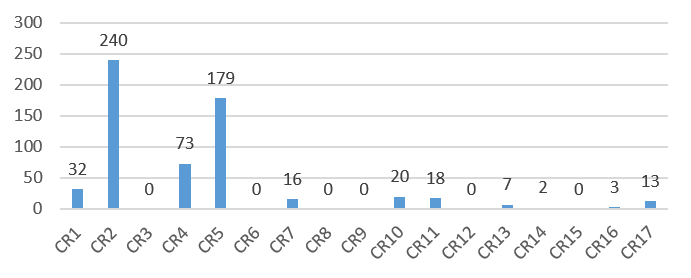
\includegraphics[width=0.9\textwidth]{./pics/chapter1pics/FrequencyICSE.png}
	%\vspace{-1em}
	\caption{Frequency of applied resolutions overall.}
	%\vspace{-1.5em}
	\label{fig:frequency_resolutions}
	\end{figure}
	
	
	\subsubsection{RQ2}
	
	%Our co-evolution approach is fully automatic and not guided by the developers, but rather by the matched patterns and their corresponding resolutions. Thus, \red{we can loose in correctness} in comparison to the  developers' manual co-evolution.
	To assess and measure the precision and recall of our automatic co-evolution, we first compared it with the manual co-evolution of the code that developers went through. 
	%To assess to what extent can our approach correctly co-evolve the code errors w.r.t. the manual co-evolution of the code that developers went through, we measured precision and recall.
	
	%Figure \ref{fig:correctness} 
	Table \ref{table:correctness} depicts the reached precision and recall of our automatic co-evolution approach for our nine case studies. We observe that the measured precision and recall varied, respectively from 48\% to 100\%, and from 51\% to 100\% reaching an average of, respectively 82\% precision and 81\% recall. 
	%
	%91,92+82,6+100+80,9+60,4+46,6+95,2+86,6+86,6 /9 = 81;20
	%91.92+82.6+100+80.9+60.4+46.6+95.2+86.6+86.6
	%
	%This means that our applied resolutions for the matched pattern usages for the code errors were correct w.r.t. the expected resolutions by the developers in \red{81\%}. 
	This shows the usefulness of the considered resolutions in Table \ref{table:ResolutionsCatalog} for the automatic co-evolution of the direct code errors in our case studies. %while meeting the developer's co-evolution needs. 
	
	\begin{table}[t]
	\caption{Measured precision and recall of our projects.}
	\label{table:correctness}
	\centering
	%
	%\small
	%\hspace*{-1em}
%	\resizebox{17.5cm}{!}{
		\begin{tabular}{
				@{\hskip3pt}l@{\hskip3pt}l@{\hskip3pt}l@{\hskip3pt}l@{\hskip3pt}l@{\hskip3pt}l@{\hskip3pt}l@{\hskip3pt}l@{\hskip3pt}l@{\hskip3pt}l@{\hskip3pt}}
			\toprule 
			Projects & P1 & P2 & P3 & P4 & P5 & P6 & P7 & P8 & P9 \\ \midrule%{2-10}
			precision & 90\%  & 80\%   & 100\%    & 81\%   & 58\%   & 48\%   & 98\%   & 93\%   & 93\% \\ \midrule
			recall & 66\%  & 83\%   & 100\%    & 75\%   & 58\%   & 51\%   & 94\%   & 100\%   & 100\% \\
			\bottomrule
		\end{tabular}
%	}
	\end{table}
	
	%\begin{figure}
	%	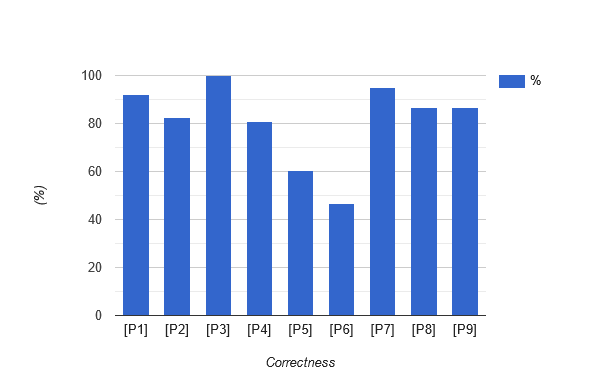
\includegraphics[width=0.6\textwidth]{pics/correctness.png}
	%\caption{Measured correctness of our projects.}
	%    \label{fig:correctness}
	%\end{figure}
	
	
	We further investigated the cause of lowering precision and recall, i.e., the cases where our automatic co-evolution did not match the expected resolutions. 
	The main observation is that several errors that could have been co-evolved by maintaining them were deleted by the developers in the manually evolved version of the code. Rather than to delete the erroneous code, our approach was able to successfully co-evolve and maintain it. 
	%
	For example, in the project \emph{P5}, we observed errors in the code due to moves of the properties \emph{maxUsedMemoryInBytes} and \emph{totalExecutionTimeInSeconds} and its rename to \emph{discoveryTimeInSeconds}. 
	%
	Our approach automatically co-evolved them and maintained the erroneous code, by renaming the setter and extending its path. Whereas, the developers' manual co-evolution consisted of deleting the impacted code. This may hint at a lack of automated co-evolution support that would have easily maintained the code in the new version rather than deleting it.  \red{Thus, our co-evolutions here are valid alternatives even if it did not match the correct manual co-evolution.}
	
	\begin{comment}
	
	\setulcolor{red}
	%,xleftmargin=0.2cm,,xrightmargin=-0cm,framexleftmargin=+6pt,frame=single
	\begin{lstlisting}[language=Java,breaklines=true,mathescape,literate={\-}{}{0\discretionary{-}{}{}},caption=Excerpt of the error in the code of the project P5.\label{lis:P5_V1}]
		//in the class Repport.java
		...
		discovery.(*\ul{setMaxUsedMemoryInBytes}*)(maxUsedMemory);
		discovery.(*\ul{setTotalExecutionTimeInSeconds}*)(...);
		...
	\end{lstlisting}
	
	\setulcolor{green}
	%,xleftmargin=0.2cm,,xrightmargin=-0cm,framexleftmargin=+6pt,frame=single
	\begin{lstlisting}[language=Java,breaklines=true,mathescape,literate={\-}{}{0\discretionary{-}{}{}},caption=Excerpt of the co-evolved error in the code of the project P5.\label{lis:P5_V2}]
		//in the class Report.java
		...
		discovery.(*\ul{getIterations().get(0).}*)  
		(*\ul{setMaxUsedMemoryInBytes}*)(maxUsedMemory);
		discovery.(*\ul{getIterations().get(0).}*) 
		(*\ul{getDiscoveryTimeInSeconds}*)(...);
		...
		
	\end{lstlisting}
	
	\end{comment}
	
	\red{It is worth noting that the order of the resolutions’ application is following the order of the treated metamodel changes. It may affect the number of iterations of Algorithm~\ref{algo :overallalgo} but it will neither affect the value of recall and precision nor the final result of the co-evolved code.}
	
	Finally, to check the behavioral effect of the co-evolution, we observed the tests' execution that we generated for the original and co-evolved code. %In total, respectively for the original and co-evolved versions. %, \red{xyz} and \red{xyz} test case were generated for the the nine projects, with \red{xyz} and \red{xyz} passing test, \red{xyz} and \red{xyz} failing tests, and \red{xyz} and \red{xyz} crashed tests due to an error. 
	Table \ref{table:test_results} depicts the test execution results. In \emph{[P1, P5, P6, P8, and P9]} similar tests were generated for the original and co-evolved versions. Whereas in \emph{[P2, P3, P7]} there were common tests as well as different generated tests, while we could also not generate tests for \emph{[P4]}. In most cases, we observe that the percentages of passing, failing, and erroneous tests were the same with no significant changes after the co-evolution. 
	Therefore, it suggests that our automatic co-evolution is behaviorally correct by not altering the code behavior of the original projects. 
	
	
	\begin{table*}[t]
	%\begin{wraptable*}{r}{5.5cm}
	\centering
	\caption{Observed test before and after co-evolution. [Legend: Before (V1) -- After (V2) ]}
	\label{table:test_results}
	%
	%\small
	%\hspace*{-2em}
	\resizebox{16cm}{!}{
		\begin{tabular}{
				@{\hskip3pt}c@{\hskip3pt}|c@{\hskip3pt}|c@{\hskip3pt}|c@{\hskip3pt}|c@{\hskip3pt}|c@{\hskip3pt}|c@{\hskip3pt}|c@{\hskip3pt}|c@{\hskip3pt}}
			\toprule 
			Projects & P1 & P2 & P3 & P5 & P6 & P7 & P8 & P9 \\ \midrule%{2-10}
			\begin{tabular}[c]{@{}l@{}}$N^{o}$ \\ tests\end{tabular} &  1987 -- 1987 & 2261 -- 2073  &  475 -- 555   & 67 -- 67  &  427 -- 427  &  142 -- 251  &  105 -- 105  &  75 -- 75 \\ \midrule
			\begin{tabular}[c]{@{}l@{}}$N^{o}$ \\ pass\end{tabular} & \begin{tabular}[c]{@{}l@{}} 826 -- 826 \\(41\% -- 41\%)\end{tabular} & \begin{tabular}[c]{@{}l@{}}  1221 -- 1161 \\ (54\% -- 56\%)\end{tabular} &\begin{tabular}[c]{@{}l@{}}  349 -- 417  \\ (73\% -- 75\%)\end{tabular}  & \begin{tabular}[c]{@{}l@{}}32 -- 32 \\ (47\% -- 47\%)\end{tabular}  &  \begin{tabular}[c]{@{}l@{}} 2 -- 2 \\(0.4\% -- 0.4\%)\end{tabular}    & \begin{tabular}[c]{@{}l@{}} 18 -- 103\\(12\% -- 41\%) \end{tabular}  &\begin{tabular}[c]{@{}l@{}}  16 -- 16\\(18\% -- 17\%) \end{tabular} & \begin{tabular}[c]{@{}l@{}} 14 -- 13 \\(15\% -- 15\%)\end{tabular}  \\ \midrule
			\begin{tabular}[c]{@{}l@{}}$N^{o}$\\ fail\end{tabular} &\begin{tabular}[c]{@{}l@{}} 14 -- 14\\ (0.7\%--0.7\%) \end{tabular}  & \begin{tabular}[c]{@{}l@{}} 36 -- 16 \\ (1,6\% -- 0,8\%)\end{tabular}  & \begin{tabular}[c]{@{}l@{}} 3 -- 3  \\(0.6\% -- 0,5\%)\end{tabular} & \begin{tabular}[c]{@{}l@{}}  2 -- 2  \\(2.9\% -- 2.9\%)\end{tabular} & \begin{tabular}[c]{@{}l@{}} 0 -- 0 \\(0\% -- 0\%)\end{tabular} & \begin{tabular}[c]{@{}l@{}}3 -- 4 \\(2.1\% -- 1.5\%)\end{tabular}  & \begin{tabular}[c]{@{}l@{}} 3 -- 3 \\(2.8\% -- 2.8\%)\end{tabular}  & \begin{tabular}[c]{@{}l@{}} 1 -- 1  \\(1.3\% -- 1.3\%)\end{tabular}\\ \midrule
			\begin{tabular}[c]{@{}l@{}}$N^{o}$\\ error\end{tabular} &\begin{tabular}[c]{@{}l@{}} 1147 -- 1147\\ (57\%--57\%) \end{tabular}&  \begin{tabular}[c]{@{}l@{}} 1004 -- 896 \\ (44\% -- 43\%)\end{tabular}  &  \begin{tabular}[c]{@{}l@{}}123 -- 135 \\(25.8\% -- 24.3\%)\end{tabular}  & \begin{tabular}[c]{@{}l@{}}33 -- 33\\(49.2\% -- 49.2\%)\end{tabular}  & \begin{tabular}[c]{@{}l@{}} 425 -- 425 \\(99.5\% -- 99.5\%)\end{tabular} &  \begin{tabular}[c]{@{}l@{}}121 -- 144 \\(85.2\% -- 57.3\%)\end{tabular} & \begin{tabular}[c]{@{}l@{}} 86 -- 86 \\(81.9\% -- 81.9\%)\end{tabular} & \begin{tabular}[c]{@{}l@{}} 60 -- 61\\(80\% -- 81.3\%)\end{tabular}\\ 
			\bottomrule
		\end{tabular}
	}
	%\end{wraptable*} 
	\end{table*}
	
	\begin{tcolorbox}[boxsep=-2pt]
	\textbf{$\boldsymbol{RQ_2}$ insights:}
	
	Our automatic co-evolution reached an average of an 82\% precision and 81\% recall.
	It was able to co-evolve and maintain erroneous code that developers unnecessarily deleted. 
	Generated tests for original and co-evolved code further showed that our co-evolution is not impacting the original code behavior w.r.t. the generated tests. 
	\end{tcolorbox}
	
	
	\begin{comment}
	
	
	\kaouter{ Discussion :1million
		1-The high-level intuition behind our approach is that
		we apply a targeted co-evolution by propagating the impacting metamodel changes only to the code errors directly, rather than browsing all code elements statically to fetch the possible impacts.
		Our automatic coevolution approach tries to mimic the developers' behavior with known resolutions when co-evolving the code errors in an “iterative way”. After the application of each resolution, the compilation unit is refreshed to get the list of the new compilation errors for the next iteration.
		
		2- the applied resolutions are related to the distribution of the impacting metamodel changes (see \ref{table:ResolutionsCatalog} ). However, there is no relation between the distribution of the applied resolution and the recall and precision that rather depends on “if” the automatic resolutions match "or not" the manual developer’s expected resolutions. Moreover, we did not randomly and synthetically choose the metamodel changes and their types in the evaluation. Rather, we took the realistic developers' evolutions of the metamodels in our selected real-world software projects.
		3- there are similarities with API migration approaches \cite{henkel2005catchup,andersen2010generic} on resolving errors in the client code, approaches do not handle all the equivalents of the impacting metamodel changes we do (\ref{table:ResolutionsCatalog}) and that occurred in our case studies. Therefore, we did not consider them as a baseline because we know apriori that too many changes would not be treated, hence, the comparison would be unfair and biased
		4-.Moreover, EMF is used for the implementation and evaluation, but our approach conceptually remains valid for other abstracted models that affect a Java code, such as in JHipster or OpenAPI.
		
	}
	
	
	%\DK{yes, i think this goes to discussion section 4.5}
	\subsection{Discussion}
	We now discuses our approach and the obtained results. 
	\end{comment}
	
	
	\subsubsection{RQ3}
	
	%\paragraph{Comparison with Quick Fixes}
	
	
	\begin{table*}[t]
	\centering
	\caption{Number of applied Quick Fixes for each project and per evolved metamodel.}
	\label{AppliedQF}
	\resizebox{16cm}{!} {
		\begin{tabular}{lllll}
			\toprule
			\begin{tabular}[c]{@{}l@{}}Evolved \\ metamodels\end{tabular} & \begin{tabular}[c]{@{}l@{}}Co-evolved \\ projects\end{tabular}  & \begin{tabular}[c]{@{}l@{}} \% of  \\eliminated \\ errors  \end{tabular} & \begin{tabular}[c]{@{}l@{}} $N^{o}$ of applied \\ Quick Fixes \end{tabular}  & Total
			\\ \midrule %& \begin{tabular}[c]{@{}l@{}} $N^{o}$ of \\applications \end{tabular}			
			
			\multirow{4}{*}{\begin{tabular}[c]{@{}l@{}}OCL \\ Pivot.ecore\end{tabular}} & $[P1]$ & 82\% 
			& \begin{tabular}[c]{@{}l@{}} 
				$  [$Create Class X$] $: 3, $ [$Create method m $] $: 27 , 
				\\  $[$Change m to m' $] $: 60,$[ $Add cast $] $: 59,
				\\  $[ $Change type (of variable or return type of method) $] $: 17,
				\\  $[ $Add unimplemented methods $] $: 43,
				\\ $[ $Create constants $] $: 15,  $[ $Remove argument $] $: 1.
			\end{tabular}  & 225\\ \cmidrule{2-5}			
			
			& $[P2]$ & 41\% 
			&\begin{tabular}[c]{@{}l@{}}
				$ [ $Create method $] $: 4,$[ $Change to m' $] $:11,\\
				$ [ $change type of var or return type $] $: 1,\\
				$ [ $Add unimplemented methods $] $: 2,
				
			\end{tabular}  & 18\\ \midrule			
			\multirow{6}{*}{\begin{tabular}[c]{@{}l@{}}Modisco \\ Benchmark.\\ecore\end{tabular}}  &  $[P3]$& 100\%
			& \begin{tabular}[c]{@{}l@{}}  
				%  $[ $  $] $
				$[ $ Create Class X  $] $: 6,  $[ $ Add unimplemented methods  $] $: 1
			\end{tabular}  & 7\\ \cmidrule{2-5}			
			
			& $[P4]$ &100\% 
			& \begin{tabular}[c]{@{}l@{}} 
				$[ $ Create Class X $] $: 2,$[ $  Create method $] $: 8,\\ $[ $ Change m to m' $] $; 5, $[ $ Remove argument $] $: 1,\\ $[ $ Add cast $] $ : 6
			\end{tabular}  & 22\\ \cmidrule{2-5}			
			
			& $[P5]$ &83\%
			& \begin{tabular}[c]{@{}l@{}}
				$[ $  Create Method $] $: 17,  $[ $ Change method m to m' $] $: 16, \\ $[ $ Remove argument $] $: 2,  $[ $ Change type of var or return type $] $: 1,\\  $[ $ Add Cast$] $: 16.
				
			\end{tabular}& 52  \\ \cmidrule{2-5}			
			
			& $[P6]$&67\% 
			& \begin{tabular}[c]{@{}l@{}}
				$[ $ Change method m to m' $] $: 4, $[ $ Add unimplemented methods  $] $: 2,\\ $[ $ Create Constant$] $:9, $[ $ change type $] $ : 2,\\$[ $ Add Cast  $] $: 6
				
			\end{tabular}& 23  \\ \midrule			
			
			\multirow{4}{*}{\begin{tabular}[c]{@{}l@{}}Papyrus \\ ExtendedTypes.\\ecore\end{tabular}} &  $[P7]$&69\%
			& \begin{tabular}[c]{@{}l@{}} 
				$[ $ Create Class X $] $: 3,  $[ $ Create method m $] $: 9,\\  $[ $ Change method m to m' $] $: 13,  $[ $Change type of var or return type  $] $: 5, \\$[ $ Add Cast $] $: 4,  $[ $Add unimplemented methods$] $: 2.
				
			\end{tabular} & 36 \\ \cmidrule{2-5}			
			
			&  $[P8]$ &93\%
			& \begin{tabular}[c]{@{}l@{}}
				$[ $ Create Class X $] $: 1,  $[ $ Create method $] $ : 14,\\ $[ $ Create Const $] $ :3,  $[ $ Add Cast$] $: 2,\\  $[ $ Change method m to m' $] $:3.
			\end{tabular} & 23 \\ \cmidrule{2-5}			
			
			&  $[P9]$ &93\% &
			
			\begin{tabular}[c]{@{}l@{}}
				$[ $ Create Class X $] $: 1,  $[ $ Create method $] $ : 14,\\ $[ $ Create Constant $] $ :3,  $[ $ Add Cast$] $: 2,\\  $[ $ Change method m to m' $] $:3.
			\end{tabular} & 23 \\ \midrule			
			Total &&&& 429 \\ \bottomrule
			
			
			%	& CS14:MPRPS                                                                                                           & \begin{tabular}[c]{@{}l@{}} $\rhd [R4]$ \\ $\rhd [R6]$ \\ $\rhd [R9]$ \end{tabular} &   \begin{tabular}[c]{@{}c@{}} 4 \\ 3 \\ 4 \end{tabular}     \\ 			
		\end{tabular}  
		
	}
	%\vspace{-0.5em}
	\end{table*}
	
	The first baseline we compare to is the quick fixes available in the IDE since they are widely used by developers to repair code errors%yu2012maintaining QF are used by developers usually to resolve compiling errors.
	%
	~\cite{10.1145/2384616.2384665}, and more importantly, they have not been compared to code co-evolution approaches before. 
	To compare with the quick fixes as a baseline, we implemented the automatic application of quick fixes as an option in our plugin. It is a variant of our Algorithm \ref{algo :overallalgo} that only applies the quick fixes on the errors. 
	The algorithm browses the errors of each compilation unit and applies the first proposed quick fix, since by default Eclipse IDE\footnote{See \emph{org.eclipse.jdt.ui.text.java.CompletionProposalComparator}} order the quick fixes by \emph{relevance}. Note that all executions herein terminated normally without any infinite loop.
	%The selection of the first quick in the list of proposals is due to the strategy of proposals ordering of eclipse. \texttt{CompletionProposalComparator} of eclipse proposes two criteria: by relevance and alphabetic order. Eclipse default settings opt for ordering by relevance.
	
	%It stops in two cases: 1) when only errors without any quick fix proposal remain, or 2) when the application of a quick fix causes an infinite loop \cite{cuadrado2018quick,khelladi2019detecting}, i.e., a cycle of applying a quick fix that causes a previously fixed error (A $\mapsto$ B $\mapsto$ A $\mapsto$ B $\mapsto$ ...).   
	%(Error A quick fixed, error B appears \textless--\textgreater 
	% Error B quick fixed, error A appears), infinite side-effect cycle. 
	
	
	
	In Table~\ref{AppliedQF}, we present the percentage of errors that quick fixes eliminated for each project, and the frequencies of each type of applied quick fixes. 
	%we give the number of quick fixes applied per type, 
	%\red{to help us to analyse the quick fixes' reaction to the different types of changes.}\todo{what ?} 
	
	While the quick fixes eliminated from 41\% to 100\% errors, we found that the precision and recall of automatic quick fixes are equal to 0, because no correction was applied as expected to the manual developers' resolutions. That is why we refer to the errors are eliminated by the quick fixes and not corrected or co-evolved. 
	For example, concerning errors caused by class or property deletion from the metamodel, renaming a class or an attribute, moving, pushing, or pulling attributes or methods from a class to another, the quick fixes proposed to create them back in their old containers. This is in contradiction of the applied metamodel changes.  
	%for some errors, the usage of the metamodel class in the code is super %interface, and when applying the first quick fix, it will create a class %and not an interface
	%duplicate case
	For errors caused by changing a variable's type, the quick fixes always suggested adding a cast with a wrong type. 
	
	%Adding a declaration or an implementation of missing or renamed method causes a major problem of polymorphism on which metamodeling is based on. In the case of adding a method declaration in an interface, all classes that implement this interface will ask to "add unimplemented method", and by applying this quick fix, an empty methods will be added. These corrections do not meet the specifications of the metamodel changes. 
	
	Unlike our approach, quick fixes do not take in consideration the context of the impacted code and the information contained in its causing metamodel changes. For example, the quick fix \texttt{create the missing method \emph{m()}} is applied no matter the metamodel change (i.e., deletion, moving, pulling, or pushing changes) or the impacted code location (i.e., statement, variable declaration, parameter, etc.). %this invocation is located in a complex statement, in a variable declaration, or in any other position in the code AST. 
	Our approach takes into account the context of the impacted code and the causing change thanks to the use of pattern matching (see Section~\ref{pattern_matching}). 
	% either the pattern MoveProperty\_UpperBoundSingle or the pattern MoveProperty Upper\_BoundMultiple is detected then
	
	
	For instance, after a move property change, the resolution $[CR7]$ or $[CR8]$ is applied, respectively. Thus, taking into consideration the embedded information in the causing metamodel change, namely the origin class, the target class, and the multiplicity of the reference between them.
	
	
	
	\begin{tcolorbox}[boxsep=-2pt]
	\textbf{$\boldsymbol{RQ_3}$ insights:}
	The automatic application of quick fixes leads to a faulty evolved code. The same type of quick fixes is applied regardless of the context of the impacted code. With 0 precision and recall, we can conclude the inability of Eclipse quick fixes to co-evolve correctly the code with the evolution of the metamodel. 
	\red{}
	
	\end{tcolorbox}
	
	
	
	\subsubsection{RQ4}
	%\paragraph{Comparison with State of the art co-evolution}
	
	%%%%%%%%%%%%%%%%%%%%Comparaison with prior work %%%%%%%%%%%%%%%%%%%%%%%%%%%%%%%%%%%%%%%%%%%%%%%%%%%%%%%%%
	%%%%%Table recall and precision per project %%%%
	\begin{table*}[t]
	%\begin{wraptable*}{r}{5.5cm}
	\centering
	\caption{Comparison between our automatic co-evolution approach and the semi-automatic co-evolution approach. [Legend: Precision(P) -- Recall(R) ]}
	\label{table:comparison_AC_vs_SC}
	%
	\normalsize
	%\hspace*{-2em}
	\resizebox{17cm}{!}{
		\begin{tabular}{
				@{\hskip3pt}c@{\hskip3pt}|c@{\hskip3pt}|c@{\hskip3pt}|c@{\hskip3pt}|c@{\hskip3pt}|c@{\hskip3pt}|c@{\hskip3pt}|c@{\hskip3pt}|c@{\hskip3pt}|c@{\hskip3pt}|c@{\hskip3pt}}
			\toprule 
			Projects & P1 & P2 & P3& P4 & P5 & P6 & P7 & P8 & P9& Total \\ \midrule%{2-10}
			\begin{tabular}[c]{@{}l@{}} Our automatic approach\end{tabular} & \begin{tabular}[c]{@{}l@{}} 90\%(P)\\ 66\%(R)\end{tabular} & \begin{tabular}[c]{@{}l@{}} 80\%(P)\\ 83\%(R)\end{tabular} &  \begin{tabular}[c]{@{}l@{}} 100\%(P) \\ 100\%(R) \end{tabular} & \begin{tabular}[c]{@{}l@{}}81\%(P) \\ 75\%(R)\end{tabular} & \begin{tabular}[c]{@{}l@{}} 58\%(P) \\ 58\%(R)\end{tabular} & \begin{tabular}[c]{@{}l@{}} 48\%(P) \\ 51\%(R)\end{tabular} & \begin{tabular}[c]{@{}l@{}} 98\%(P) \\ 94\%(R)\end{tabular} & \begin{tabular}[c]{@{}l@{}}  93\%(P) \\ 100\%(R)\end{tabular} & \begin{tabular}[c]{@{}l@{}} 93\%(P) \\ 100\%(R)\end{tabular}
			& \begin{tabular}[c]{@{}l@{}} 82\%(P) \\ 81\%(R)\end{tabular}
			\\ \midrule
			
			\begin{tabular}[c]{@{}l@{}} \textbf{Semi-automatic approach \cite{Khelladi2020}}\end{tabular} & \begin{tabular}[c]{@{}l@{}}92\%(P) \\ 92\%(R)\end{tabular} & \begin{tabular}[c]{@{}l@{}} 93\%(P) \\ 86\%(R)\end{tabular} &\begin{tabular}[c]{@{}l@{}} 100\%(P) \\ 100\%\end{tabular}  & \begin{tabular}[c]{@{}l@{}}100\%(P) \\ 100\%(R) \end{tabular}  &  \begin{tabular}[c]{@{}l@{}}100\%(P) \\ 100\%(R)\end{tabular}    & \begin{tabular}[c]{@{}l@{}} 48\%(P) \\ 48\%(R)\end{tabular}  &\begin{tabular}[c]{@{}l@{}} 100\%(P) \\ 100\%(R)\end{tabular} & \begin{tabular}[c]{@{}l@{}}100\%(P) \\ 100\%(R)\end{tabular} & \begin{tabular}[c]{@{}l@{}}100\%(P) \\ 100\%(R)\end{tabular}   & \begin{tabular}[c]{@{}l@{}}92\%(P) \\ 91\%(R)\end{tabular}  \\
			\bottomrule
			
		\end{tabular}
	}
	
	%\end{wraptable*} 
	\end{table*}
	
	%%%% Text about comparison AC vs SC
	% we treat more changes. the impact analysis is not the same.
	
	
	
	We now compare our approach to the state of the art of metamodel and code co-evolution, namely our previous work \cite{Khelladi2020}. It runs an impact analysis to trace the impacts in the code, while we rely on the compilation errors after regenerating the code API from the evolved metamodel. 
	We also consider an additional change of Pull property and add a new resolution for it ($CR14$). 
	We further distinguish with our previous work by checking behavioral correctness with tests (before/after co-evolution) and by comparing to two baselines. 
	Yet, the main difference is it being semi-automatic requiring intervention to decide between alternative resolutions to co-evolve the code, while we fully automate this decision based on our pattern matching process. Thus, intuitively, it will likely perform better than a fully automatic co-evolution. RQ4 aims to measure this difference.  
	
	%The semi-automatic approach of code co-evolution of Khelladi et al. \cite{Khelladi2020} starts by change detection and an impact analysis. This approach takes into account the types of changes listed in Table \ref{mmchanges}, except for the "Pull property" change type. While the impacted parts in code, in our approach, consist of compiling errors, Khelladi et al. \cite{Khelladi2020} proceed by a static analysis without compilation. Each evolved metamodel is traced through the AST of the generated code elements and their usages in the AST of the additional code. The impacted nodes are then coevolved using the catalog of resolutions \ref{table:ResolutionsCatalog} ( that does not include $CR14$). 
	%Our approach is 100\% automatic thanks to the pattern matching process \ref{pattern_matching}. In the case of an impact that supports more than one resolution, Khelladi et al. give the developer the choice to select one of the possible resolutions.
	%This semi-automatic approach is evaluated on the nine projects described in Table \ref{CaseStudies_CoEvolution}. Unlike our evaluation, Khelladi et al. used only precision and recall metrics in their evaluation process, without any other checking of the behavioral correctness of their semi-automatic co-evolution approach. 
	Table \ref{table:comparison_AC_vs_SC} shows precision and recall values of our approach and the semi-automatic co-evolution approach~\cite{Khelladi2020}. 
	We notice that the semi-automatic co-evolution approach~\cite{Khelladi2020} outperforms our automatic co-evolution approach by a small margin in terms of precision and recall. % ( 92\% over 82\%) and recall(91\% over 81\%). However, the margin between the values remains small. 
	On average, we had 82\% precision and 81\% recall in full automatic co-evolution compared to 92\% precision and 91\% recall in semi-automatic co-evolution. 
	This is due to the fact that our approach favors the least deletion when possible $[CR1]$ over $[CR3]$, or $[CR4]$ over $[CR2]$, while the semi-automatic approach favors integral deletions $[CR3]$ over $[CR1]$, or $[CR2]$ over $[CR4]$. %, and this integral deletion matches the developers' co-evolved version.
	Overall, we observe that the trade-off between full and semi-automatic co-evolution leads to only a reduction of -10\% in precision and recall while still maintaining them at a high level ($>$ 81\%). This small reduction in performance provides a bigger benefit of speeding up the co-evolution and removing the burden of manual intervention from developers on every code error. Indeed, rather than spending time in guiding the co-evolution at every error, developers can automatically perform it in couples of minutes, in particular, if thousands of errors must be co-evolved after metamodel evolution.
	
	
	\begin{tcolorbox}[boxsep=-2pt]
	\textbf{$\boldsymbol{RQ_4}$ insights:}
	Fully automating metamodel and code co-evolution performs less than a semi-automatic co-evolution, but still gives a high precision and recall of ($>$ 81\%) while removing the burden of manual intervention from developers on every code error to co-evolve. 
	\end{tcolorbox}
	
	% Tests for correctness checking
	% Precision, Recall
	%%%%%%%%%%%%%%%%%%%%%%%%%%%%%%%%%%%%%%
	
	% describe the approach
	\subsection{Discussion and limitations}
	This section discusses the approach and the observed results. 
	
	The high-level intuition behind our approach is that we apply a targeted co-evolution by propagating the impacting metamodel changes only to the code errors directly, rather than browsing all code elements statically to fetch the possible impacts.
	Our automatic co-evolution approach tries to mimic the developers' behavior with known resolutions when co-evolving the code errors in an “iterative way”. After the application of each resolution, the list of errors %compilation unit 
	is refreshed to get the list of the new compilation errors for the next iteration.
	% relation betsween the input and the output of the evaluation
	
	Moreover, Table \ref{AppliedResolutions} shows the distribution of applied resolutions. It is related to the distribution of the impacting metamodel changes (see Table~\ref{table:ResolutionsCatalog}) since for a given impacting change, a specific set of resolutions can be applied. 
	However, there is no relation between the distribution of the applied resolution and the recall and precision, which depends more on 'if' the automatic resolutions match "or not" the manual developer’s expected resolutions. Moreover, we did not randomly and synthetically choose metamodel changes and their types in the evaluation. Rather, we took the realistic developers' evolutions of the metamodels in our selected real-world software projects. Thus, we did not influence the applied resolutions, which correspond only to the metamodel changes. Of course, having a different distribution of metamodel changes would result in a different distribution of applied resolutions. 
	
	Finally, we handled the evolution of one metamodel at once to co-evolve its impacts. Handling multiple metamodels is an interesting case, but is out-of-scope in this dissertation. Nonetheless, the first favorable scenario we can currently handle is to treat the multiple metamodels in sequence when they are independent of each other. The main limitation is in a second scenario where there are dependencies between the multiple metamodels. For example, a change "set type to T" in a metamodel A referencing a change "add T" in a metamodel B. Herein, the solution would be to find the order of metamodels in which to handle the co-evolution in sequence. This is left as future work. 
	
	\section{Threats to Validity}\label{ch1_threat}
	\noindent This section discusses threats to validity \cite{wohlin2012experimentation}.
	
	\subsection{Internal Validity.} To provoke the code errors, we had to replace the original metamodel evolution and to regenerate the code API. To reduce any bias in the source of errors, we decided to evolve one metamodel at a time. This increases the confidence in the source of the errors, and hence, their co-evolution. Dealing with conflicting errors that can mask each other due to the simultaneous evolution of several metamodels is left for future work.  
	Moreover, to measure the correctness, we analyzed the developers' manual co-evolution.
	To reduce the risk of misidentifying an expected resolution, for each impacted part of the code, we investigated the entire co-evolved class. If we did not find it, we further searched in other classes in case the original impacted part of the code was moved into another class. Thus, our objective was to reduce the risk of missing any correspondence between an error in the original code and its evolved version. Moreover, as our co-evolution relies on the quality of detected metamodel changes, we analyzed each detected change and checked whether it occurred between the original and evolved metamodels. This alleviates the risk of relying on an incorrect metamodel change that would degrade the pattern matching. 
	Note that the order of changes taken as input does not influence our co-evolution, but the order of errors we treat may affect the distribution of the applied resolutions. However, we took the order in which the errors were detected. 
	Finally, besides the manual checking of the co-evolved code, we used Evosuite as a test suites generation tool that has shown its efficiency in
	test generation as a state-of-the-art tool~\cite{DANGLOT2019110398,https://doi.org/10.1002/stvr.1601}. The main reason is that our projects did not have manually written tests. However, automatic test
	generation can even be more advantageous herein. Indeed, it generates tests for all
	public methods, whereas developers tend to manually write few tests for only some targeted methods. Thus, if relying only on manually written tests, there is a high risk of not assessing the behavioral correctness of many cases of code co-evolutions that are not covered by test cases. Despite the fact that generated tests can be better for our approach and its results allow us to measure the behavioral correctness of the co-evolution, %it is still not sufficient as it cannot replace the manual written tests. Further studies are needed here}.
it still can be combined with manual written tests.


\subsection{External Validity.} We implemented and evaluated our approach for EMF and Ecore metamodels and Java code. %As EMF metamodels rely on MOF \cite{MOF241} and object-oriented elements that can 
%Other object-oriented languages use different syntax but conceptually use the same constructions as in Java, such as C\# or C++.
Although co-evolution could theoretically be applicable for other languages, such as C\# or C++, we cannot generalize our results. Further experimentation on other languages is necessary. However, the only requirement to apply our approach to other languages is to parse the ASTs of the erroneous code and to adapt our resolutions to the new ASTs' structure.  

Furthermore, the evaluation was carried out on Eclipse projects in three languages. Thus, we cannot generalize our findings to other software languages and their implementations. However, our approach could be used to co-evolve Java code added on top of a generated code from a domain model, \eg from a UML class diagram or an entity model. %, such as JHipster that generates a complete and modern Web app or microservice architecture based on a domain model and a set of architectural choices. 
Nonetheless, more evaluations are still necessary. %\footnote{https://www.jhipster.tech/}

\subsection{Conclusion Validity.} Our evaluation showed promising results with an automatic code co-evolution that is fast and useful, with an average of~82\% precision and~81\% recall varying from~48\% to~100\%. The results also showed the usefulness of our approach and the resolutions proposed in our catalog in Table \ref{table:ResolutionsCatalog}. However, even though we evaluated it on nine projects with complex metamodel evolution, we plan to further evaluate on more case studies to have more insights and statistical evidence.  %further evaluation is needed on more case studies.
\begin{comment}
	
\end{comment}


\section{Conclusion}\label{ch1_conclusion}

In this chapter, we presented an approach to automatically co-evolve code when metamodels evolve. It relies on a pattern matching algorithm to match the different pattern usages of the metamodel generated code elements in the additional erroneous code. Once a direct error in the code is matched with a pattern usage, we can co-evolve it with its corresponding resolution. 
For indirect errors that cannot be matched, we apply the available quick fix to repair them. 
%
Our code co-evolution was evaluated on nine projects and three metamodels from three Eclipse EMF implementations. After re-generating the code API from the evolved version of the metamodel, hence, causing~837 errors in the additional code.
For the~771 direct errors, our automatic co-evolution approach was able to match 631 pattern usages and to apply~631 resolutions. It showed to be efficient and useful in co-evolving all direct errors in the code with an average of~82\% precision and~81\% recall varying from~48\% to~100\%. All~66 indirect errors were resolved by calling~5 quick fixes. Moreover, we checked the behavioral correctness of our approach by using test suites before and after code co-evolution. We observed that the percentage of passing, failing, and erroneous tests remained stable with insignificant variations in some projects. Thus, suggesting the behavioral correctness of the co-evolution. Finally, we found that the quick fixes are not able to correctly co-evolve the code. This is because they cannot exploit the context of the impacted code and relate it to the changes of the metamodel. 
\red{We also found that fully automating metamodel and code co-evolution performs less than a semi-automatic co- evolution, but still gives a high precision and recall of ($>$ 81\%) while removing the burden of manual intervention from developers on every code error to co-evolve.}


In summary, our work presents the following contributions :
1/ A fully automatic code co-evolution approach due to Ecore metamodel evolution based on pattern matching. 
2/ A prototype implementation of an Eclipse plugin to show the efficiency of our approach. % available publicly\footnote{\url{https://figshare.com/s/8986914e924300be77da}}.
3/ An evaluation based on four actions: 1) Measuring the co-evolution correctness. 2) Verifying the behavioral correctness using unit tests running before and after automatic code co-evolution. 3) Comparison with the state-of-the art semi-automatic co-evolution approach~\cite{Khelladi2020}. 4) Comparison with Quick Fixes popular tool.



%As future work, we first plan to explore ordering the errors in the code before co-evolving them. In fact, we co-evolve the errors in the same order they are retrieved by the JDT. Thus, we will investigate whether it could reach better correctness with faster co-evolution or not. 
%
%Finally, we plan to extend our resolutions with a replace resolution, based on distance metrics to find element replacements to co-evolve the code. \red{After that, we can rely on our approach to extend it with a search-based heuristics, such as genetic algorithms to explore different paths of co-evolution, in contrast to a single path that we compute in this paper. In particular, to explore the different alternative resolutions of $CR1-CR4$.}  

%
%a\kaouter{}
%\DK{either we put it as future work, maybe even in discussion above 4.5, and then refer to it here and say future work.}
%
%Finally, we will evaluate our approach on more case studies and on the case of simultaneous multiple metamodel evolution. 
%\section*{Acknowledgments.} The research leading to these results has received funding from the \emph{RENNES METROPOLE} under grant \emph{AIS no. 19C0330} and from \emph{ANR} agency under grant \emph{ANR JCJC MC-EVO$^{2}$ 204687}.

%\newpage

%\begin{quote}


%\end{quote}




\chapter[ceci est un long titre]{Nom du chapitre 2}

Lorem ipsum dolor sit amet, «~consectetuer~» adipiscing elit. Maecenas fermentum, elit non lobortis cursus, orci velit suscipit est, id mollis turpis mi eget orci. Ut aliquam sollicitudin metus. Mauris at sapien sed sapien congue iaculis. Nulla lorem urna, bibendum id, laoreet iaculis, nonummy eget, massa. Phasellus ullamcorper commodo velit. Class aptent taciti sociosqu ad litora torquent per «~conubia nostra~», per inceptos hymenaeos. Phasellus est. Maecenas felis augue, gravida quis, porta adipiscing, iaculis vitae, felis. Nullam ipsum. Nulla a sem ac leo fringilla mattis. Phasellus egestas augue in sem. Etiam ac enim non mauris ullamcorper scelerisque. In wisi leo, malesuada vulputate, tempor sit amet, facilisis vel, velit. Mauris massa est, sodales placerat, luctus id, hendrerit a, urna. Nullam eleifend pede eget odio. Duis non erat. Nullam pellentesque\footcite[225]{Doule1887}.

\section{Première section du chapitre}

\subsection{Première sous-section}

Cras molestie. Curabitur id urna. Suspendisse tempor. Aliquam erat volutpat. Aliquam erat volutpat. Nam ultricies metus sit amet erat\footnote{Mauris neque odio, ornare id, rhoncus non, sollicitudin sed, lectus. Phasellus et dolor. Aenean ullamcorper risus id libero. Pellentesque ac sem eget libero aliquam tincidunt. Suspendisse neque.}. Suspendisse eget ipsum ut purus imperdiet suscipit. Mauris sed urna at diam volutpat placerat. Nulla vitae tortor. Nulla sed nisl.

Morbi lorem. Etiam scelerisque rhoncus orci. Nunc elementum ante ac leo. Vestibulum venenatis dictum nunc. Donec turpis est, dictum nec\footcite[228]{Drocher2006}, fringilla nec, cursus id, quam. In nibh orci, porttitor ut, rutrum id, faucibus vitae, leo. Donec ut wisi. Vivamus ornare, lorem quis tristique dapibus, nulla nisl nonummy libero, vitae luctus sem felis vel nisl. Suspendisse lectus lacus, ultricies vitae, feugiat et, hendrerit in, quam. Pellentesque porttitor enim at lectus. Praesent viverra laoreet velit. Mauris neque odio, ornare id, rhoncus non, sollicitudin sed, lectus. Phasellus et dolor. Aenean ullamcorper risus id libero. Pellentesque ac sem eget libero aliquam tincidunt. Suspendisse neque. Curabitur egestas neque ultrices nisl. Nulla bibendum augue et tellus. Duis ultrices convallis est.

Lorem ipsum dolor sit amet, consectetuer adipiscing elit. Maecenas fermentum, elit non lobortis cursus, orci velit suscipit est, id mollis turpis mi eget orci. Ut aliquam sollicitudin metus. Mauris at sapien sed sapien congue iaculis. Nulla lorem urna, bibendum id, laoreet iaculis, nonummy eget, massa. Phasellus ullamcorper commodo velit. Class aptent taciti sociosqu ad litora torquent per conubia nostra, per inceptos hymenaeos. Phasellus est. Maecenas felis augue, gravida quis, porta adipiscing, iaculis vitae, felis. Nullam ipsum. Nulla a sem ac leo fringilla mattis. Phasellus egestas augue in sem. Etiam ac enim non mauris ullamcorper scelerisque. In wisi leo, malesuada vulputate, tempor sit amet, facilisis vel, velit. Mauris massa est, sodales placerat, luctus id, hendrerit a, urna. Nullam eleifend pede eget odio. Duis non erat. Nullam pellentesque.


\subsection{Deuxième sous-section}

Morbi lorem. Etiam scelerisque rhoncus orci. Nunc elementum ante ac leo. Vestibulum venenatis dictum nunc. Donec turpis est, dictum nec, fringilla nec, cursus id, quam. In nibh orci, porttitor ut, rutrum id, faucibus vitae, leo. Donec ut wisi. Vivamus ornare, lorem quis tristique dapibus, nulla nisl nonummy libero, vitae luctus sem felis vel nisl. Suspendisse lectus lacus, ultricies vitae, feugiat et, hendrerit in, quam. Pellentesque porttitor enim at lectus. Praesent viverra laoreet velit. Mauris neque odio, ornare id, rhoncus non, sollicitudin sed, lectus. Phasellus et dolor. Aenean ullamcorper risus id libero. Pellentesque ac sem eget libero aliquam tincidunt. Suspendisse neque. Curabitur egestas neque ultrices nisl. Nulla bibendum augue et tellus. Duis ultrices convallis est.

Lorem ipsum dolor sit amet, consectetuer adipiscing elit. Maecenas fermentum, elit non lobortis cursus, orci velit suscipit est, id mollis turpis mi eget orci. Ut aliquam sollicitudin metus. Mauris at sapien sed sapien congue iaculis. Nulla lorem urna, bibendum id, laoreet iaculis, nonummy eget, massa. Phasellus ullamcorper commodo velit. Class aptent taciti sociosqu ad litora torquent per conubia nostra, per inceptos hymenaeos. Phasellus est. Maecenas felis augue, gravida quis, porta adipiscing, iaculis vitae, felis. Nullam ipsum. Nulla a sem ac leo fringilla mattis. Phasellus egestas augue in sem. Etiam ac enim non mauris ullamcorper scelerisque. In wisi leo, malesuada vulputate, tempor sit amet, facilisis vel, velit. Mauris massa est, sodales placerat, luctus id, hendrerit a, urna. Nullam eleifend pede eget odio. Duis non erat. Nullam pellentesque.

Lorem ipsum dolor sit amet, consectetuer adipiscing elit. Maecenas fermentum, elit non lobortis cursus, orci velit suscipit est, id mollis turpis mi eget orci. Ut aliquam sollicitudin metus. Mauris at sapien sed sapien congue iaculis. Nulla lorem urna, bibendum id, laoreet iaculis, nonummy eget, massa. Phasellus ullamcorper commodo velit. Class aptent taciti sociosqu ad litora torquent per conubia nostra, per inceptos hymenaeos. Phasellus est. Maecenas felis augue, gravida quis, porta adipiscing, iaculis vitae, felis. Nullam ipsum. Nulla a sem ac leo fringilla mattis. Phasellus egestas augue in sem. Etiam ac enim non mauris ullamcorper scelerisque. In wisi leo, malesuada vulputate, tempor sit amet, facilisis vel, velit. Mauris massa est, sodales placerat, luctus id, hendrerit a, urna. Nullam eleifend pede eget odio. Duis non erat. Nullam pellentesque.

\section{Conclusion du second chapitre}


Lorem ipsum dolor sit amet, consectetuer adipiscing elit. Maecenas fermentum, elit non lobortis cursus, orci velit suscipit est, id mollis turpis mi eget orci. Ut aliquam sollicitudin metus. Mauris at sapien sed sapien congue iaculis. Nulla lorem urna, bibendum id, laoreet iaculis, nonummy eget, massa. Phasellus ullamcorper commodo velit. Class aptent taciti sociosqu ad litora torquent per conubia nostra, per inceptos hymenaeos. Phasellus est. Maecenas felis augue, gravida quis, porta adipiscing, iaculis vitae, felis. Nullam ipsum. Nulla a sem ac leo fringilla mattis. Phasellus egestas augue in sem. Etiam ac enim non mauris ullamcorper scelerisque. In wisi leo, malesuada vulputate, tempor sit amet, facilisis vel, velit. Mauris massa est, sodales placerat, luctus id, hendrerit a, urna. Nullam eleifend pede eget odio. Duis non erat. Nullam pellentesque.

Lorem ipsum dolor sit amet, consectetuer adipiscing elit. Maecenas fermentum, elit non lobortis cursus, orci velit suscipit est, id mollis turpis mi eget orci. Ut aliquam sollicitudin metus. Mauris at sapien sed sapien congue iaculis. Nulla lorem urna, bibendum id, laoreet iaculis, nonummy eget, massa. Phasellus ullamcorper commodo velit. Class aptent taciti sociosqu ad litora torquent per conubia nostra, per inceptos hymenaeos. Phasellus est. Maecenas felis augue, gravida quis, porta adipiscing, iaculis vitae, felis. Nullam ipsum. Nulla a sem ac leo fringilla mattis. Phasellus egestas augue in sem. Etiam ac enim non mauris ullamcorper scelerisque. In wisi leo, malesuada vulputate, tempor sit amet, facilisis vel, velit. Mauris massa est, sodales placerat, luctus id, hendrerit a, urna. Nullam eleifend pede eget odio. Duis non erat. Nullam pellentesque.


\chapter{An Empirical Study on Leveraging LLMs for Metamodels and Code Co-evolution}
\label{chapitre3}
As I explained in section ?? of the background and section ?? of the state of the art, LLMs are widely explored in Model-Driven Engineering and Software Engineering, but no existing study evaluated the LLMs capabilities 
to support developers in the problem of metamodels and code co-evolution. 
In this chapter, I present a novel approach to mitigate the challenge of metamodel evolution impacts on the code using LLMs. 
%Chatgpt as LLM 
Our approach is based on prompt engineering, where we design and generate natural language prompts to best co-evolve the impacted code due to the metamodel evolution. I first explain how a prompt template is structured, then how I investigated the usefulness of this template structure. 

  Section 2 presents a motivating example to illustrate the problem of metamodels and code co-evolution. Section 3 presents our approach for generating prompts and details the prototype implementation.  Section 4 details our followed methodology in this empirical study. This section assesses the usefulness of my approach and compares ot to IDE quick fixes as a baseline. Section 5 reports on the obtained results and discusses threats to validity.Finally, Section 7 concludes this chapter. 

\section{Motivating example}
\label{example}


%To have an overview of the challenge we work on, 
To illustrate the adressed challenge, let us have an example. 
Figure \ref{fig: BMM} shows an excerpt of the  version ~0.9.0 of "Modisco Discovery Benchmark" metamodel. %\footnote{\url{https://git.eclipse.org/r/plugins/gitiles/modisco/org.eclipse.modisco/+/refs/tags/0.12.1/org.eclipse.modisco.infra.discovery.benchmark/model/benchmark.ecore}}.
Modisco is an academic initiative project implemented in the Eclipse platform that has evolved numerous times in the past to support the development of model-driven tools, reverse engineering, verification, and transformation of existing software systems \cite{bruneliere2010modisco,bruneliere2014modisco}.
%consisting of 10 classes in the version of~0.9.0.
Figure \ref{fig: BMM} illustrates  some of the domain concepts \textbf{Discovery}, \textbf{Project}, and \textbf{ProjectDiscovery}  used for the discovery and reverse engineering of an existing software system. 
From these metaclasses, a first code API is generated, containing Java interfaces and their implementation classes, a factory, a package, etc. %(details of created files in table \ref{table: locationofMMelemen}). 
Listing \ref{lis:Modisco_Code_API_V1} shows a snippet of the generated Java interfaces and classes from the metamodel in Figure \ref{fig: BMM}. 

The generated code API is further enriched by the developers with additional code functionalities in the "Modisco Discovery Benchmark" project and its dependent projects as well.
For instance, by implementing the methods defined in metaclasses and advanced functionalities in new classes.
% (\eg language services, tooling, \dots).
Listing \ref{lis:Modisco_Code_External_V1} shows the two classes \texttt{Report} and \texttt{JavaBenchmarkDiscoverer} of the additional code ({\small\boxed{Line~4,8}} in the same project "Modisco Discovery Benchmark" and in another dependent project, namely the "Modisco Java Discoverer Benchmark" project).
%, namely the classes \texttt{CDOProjectDiscoveryImpl} and \texttt{JavaBenchmarkPackageImpl}. 
%
%One of the dependent projects on the Modisco discovery benchmark metamodel is Java Benchmark Discoverer. From this project, as an example, we select 3 classes shown in Listing \ref{lis:Modisco_Code_External_V1}. 
%
%In particular, the classes \texttt{CDOProjectDiscoveryImpl} and \texttt{JavaBenchmarkPackageImpl}, and \texttt{JavaDiscoveredProjectImpl}, which handles information and statistics about CDO and Java project. 
%
%the class \textit{CDOProjectDiscoveryImpl} gives information and statistics about CDO project Discovery. 
%Another dependent class \textit{JavaBenchmarkPackageImpl} that creates and initializes the package' methods %for Package models
%( or Benchmark models ? non). The last class is
%\textit{JavaDiscoveredProjectImpl} that contains different information and statistics about java discovered project. 
%The method \textit{initializePackageContents} (line 12) retrieves a \textit{ProjectDiscovery} instance to initialize the classes of the Java Benchmark Package. The method \textit{eBaseStructuralFeatureID} (line 24) returns the structural identifier of the feature relying on the type of its class.  
%
%From version 0.9.0 to 0.11.0, 
In version~0.11.0, the "Modisco Discovery Benchmark" metamodel evolved with several significant changes, among which the following impacting changes: \emph{1)} Renaming the property \texttt{DicoveryDate} of the class  \texttt{JavaBenchmarkDiscoverer} to \texttt{DiscoveryDate}, and \emph{2)} Moving the property \emph{discoveryTimeInSeconds} from metaclass \texttt{Discovery} to \texttt{DiscoveryIteration}.

%To analyze the consequences of the metamodel evolution on the additional code, we track the impacts of the following metamodel changes:
%\begin{enumerate}%[noitemsep,nolistsep]



%\item Pulled the reference \textit{discoveries} from metaclass \texttt{DiscoveredProject} to \texttt{Benchmark}.
\begin{comment}
	
	
	\begin{itemize}
		\item \emph{1)} Renaming the property \texttt{DicoveryDate} of the class  \texttt{JavaBenchmarkDiscoverer} to \texttt{DiscoveryDate}. % and \texttt{DiscoveredProject}.
		
		\item \emph{2)} Moving the property \emph{discoveryTimeInSeconds} from metaclass \texttt{Discovery} to \texttt{DiscoveryIteration}. 
	\end{itemize} %\DK{maybe choose another rename and move ? averageSaveTimeInSeconds ?}
\end{comment}

\begin{figure}
	
	\centering
	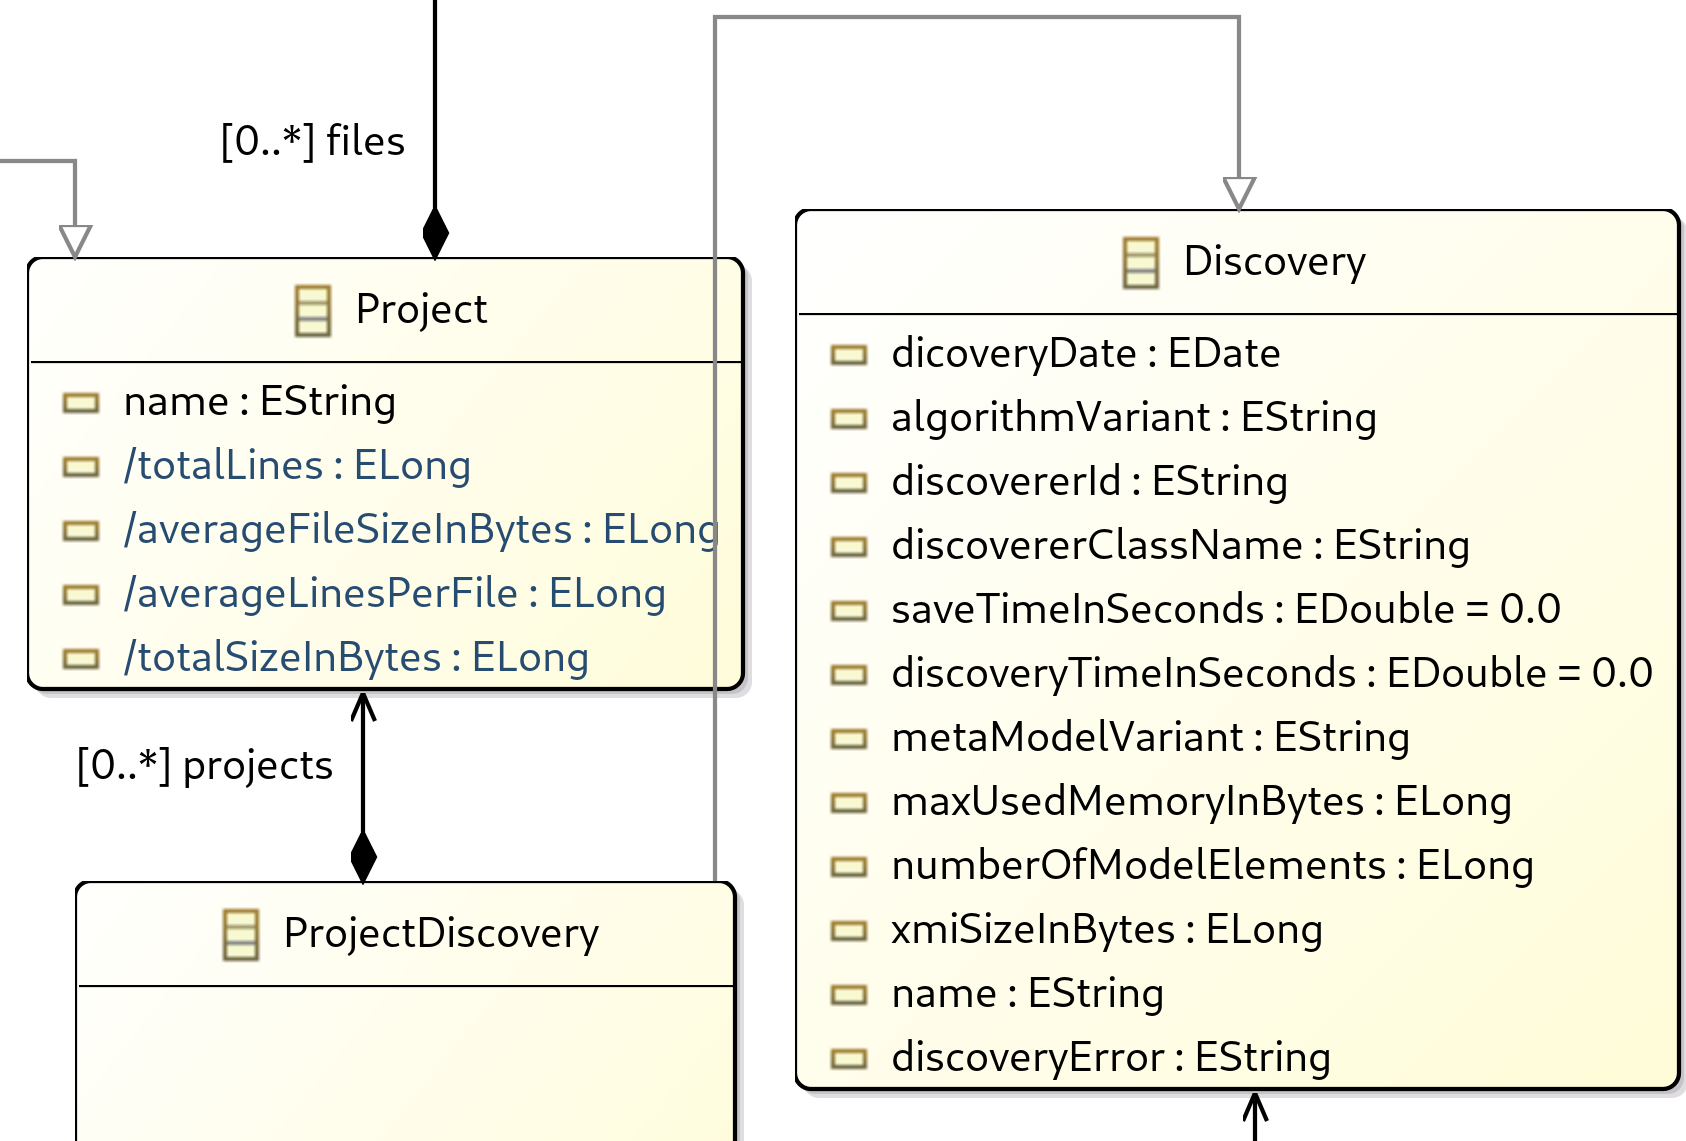
\includegraphics[width=0.45\textwidth]{./pics/chapter3pics/example.PNG}
	\caption{Excerpt of Modisco Benchmark metamodel in version 0.9.0.}
	\label{fig: BMM}
	%\vspace{-5mm}
\end{figure}



After applying these modifications, the code of Listing \ref{lis:Modisco_Code_API_V1} is re-generated from the evolved version of the metamodel, which impacts the existing additional code depicted in Listings \ref{lis:Modisco_Code_External_V1}. 

\begin{lstlisting}[language=Java,breaklines=true,mathescape,literate={\-}{}{0\discretionary{-}{}{}},caption=Excerpt of the generated code in org.eclipse.modisco.infra.discovery.benchmark.,label={lis:Modisco_Code_API_V1}]
	//Discovery Interface
	public interface Discovery extends EObject {
		double getTotalExecutionTimeInSeconds();
		void setTotalExecutionTimeInSeconds(double value);
		...
	}
	//Project Interface
	public interface ProjectDiscovery extends Discovery {...}
	//DiscoveryImpl Class
	public class DiscoveryImpl extends EObjectImpl implements Discovery {
		public double getTotalExecutionTimeInSeconds() {...}
		public void setTotalExecutionTimeInSeconds(double totalExecTime) {...}
		...
	}
\end{lstlisting}
%xleftmargin=0.2cm,xrightmargin=0cm,framexleftmargin=+6pt,frame=single,
\begin{lstlisting}[language=Java,breaklines=true,mathescape,literate={\-}{}{0\discretionary{-}{}{}},caption=Excerpt of the additional code V1.,label={lis:Modisco_Code_External_V1}]
	
	public class Report {
		...
		discovery.(*\ul{setDiscoveryTimeInSeconds}*)(...);
	}
	
	public class JavaBenchmarkDiscoverer extends AbstractModelDiscoverer<IFile> {
		...
		discovery.(*\ul{setDicoveryDate}*)(new Date());
		...
	} 
\end{lstlisting}


%%%%%%%%%%%%%%%%%%%%%%%%%%%%%%%%%%%%%%%%%%%%%%%%%%%%%%%%%%%
%%                   Now the evolved code                %%
%%%%%%%%%%%%%%%%%%%%%%%%%%%%%%%%%%%%%%%%%%%%%%%%%%%%%%%%%%%
\setulcolor{green} 
%\setstcolor{green}
%\setstcolor{green}
%,xleftmargin=0.2cm,,xrightmargin=-0cm,framexleftmargin=+6pt,frame=single
\begin{lstlisting}[language=Java,breaklines=true,mathescape,literate={\-}{}{0\discretionary{-}{}{}},caption=Excerpt of the additional code V2.,label={lis:Modisco_Code_External_V2}]
	
	public class Report {
		...
		discovery.(*\ul{getIterations().get(0).}*) 
		(*\ul{setDiscoveryTimeInSeconds}*)(...);
		...
	}
	
	public class JavaBenchmarkDiscoverer extends AbstractModelDiscoverer<IFile> {
		...
		discovery.(*\ul{setDiscoveryDate}*)(new Date());
		...
	}
\end{lstlisting}




The resulting errors in the original code in version 0.9.0 are underlined in red in Listing \ref{lis:Modisco_Code_External_V1}. Listing \ref{lis:Modisco_Code_External_V2} presents the final result of the manual developer's co-evolution in version 0.11.0. The co-evolved code is underlined in green. 
% Expected co-evolution ?
The changes \textit{rename} of the property \textit{ DicoveryDate} and the \textit{move} of the property \emph{discoveryTimeInSeconds} impact their usages ({\small\boxed{Line~4,8}} in Listing~\ref{lis:Modisco_Code_External_V1}). The impact of renaming \textit{ DicoveryDate} is co-evolved by replacing \textit{setDicoveryDate} by \textit{setDiscoveryDate}. The impact of moving the property \emph{discoveryTimeInSeconds} is co-evolved by extending the call path of the method \emph{setDiscoveryTimeInSeconds} through the reference \textit{iterations} by calling the method \textit{getIterations} and getting the first element of the returned list of DiscoveryIteration objects.

%The above examples show the importance of correctly matching the different code usages of the generated code with the metamodel evolution changes to co-evolve them with the appropriate resolutions.  
Developers unfortunately manually co-evolve the code, which is tedious, error-prone, and time-consuming. 
One help developers get is from the IDE and the provided quick fixes. For example, when using Eclipse quick fixes to co-evolve these errors, it suggests creating the method \texttt{setDiscoveryTimeInSeconds} in the class \texttt{Discovery}, which does not meet the required co-evolutions shown in Listing~\ref{lis:Modisco_Code_External_V2}.

With the ever-growing popularity and promising results of LLMs, a developer can prompt an LLM to suggest a co-evolution. 
For example, 
%To motivate more our work, 
we asked ChatGPT to co-evolve the error resulted from moving the property \emph{discoveryTimeInSeconds} by giving the erroneous code ({\small\boxed{Line~4}} in Listing~\ref{lis:Modisco_Code_External_V1})  with the message of the error taken from eclipse Problems window. This is the first intuition when using ChatGPT because the developer does not know necessarily the metamodel change causing the error and finding it due to the abstraction gap is a tedious and error-prone task. Figure \ref{fig: chatgptanswer} shows that ChatGPT proposes to create a method named \emph{setDiscoveryTimeInSeconds} in the class \emph{Discovery}, which is totally wrong because it does not fit the causing change. 

Our Hypothesis is that the LLM fails because our problem is more complex than simply repairing a code error. It must understand the original impacting metamodel change traced to the code error, as well as the abstraction gap between the two artefacts of metamodels and code. After improving the prompt, \LLM succeeded to give the right resolution as show in Figure \ref{fig: chatgptimprovedanswer}.
Our vision is that this contextual rich information must be injected in the prompt.
Thus, the quality of the prompt is a key for the LLM to solve this problem of metamodels and code co-evolution. %Indeed, it is a hard problem due to the abstraction gap between the two artefacts of metamodels and code. This context should be part of the prompt as well as the impacting metamodle change that must be traced to the code error. 

%by giving only the errouneous ({\small\boxed{Line~4}} in Listing~\ref{lis:Modisco_Code_External_V1}). Chatgpt answer in this case was totaly wrong. Thus, we injected the change information in the request and asked Chatgpt to coevolve the same error. Figure \ref{fig: chatgptanswer} shows that even adding the change information did not help chatgpt to find the right resolution.
%
The next section presents our contribution for a contextualized information rich prompts-based co-evolution of metamodel and code using LLMs.  


\begin{figure}[t]
	\centering
	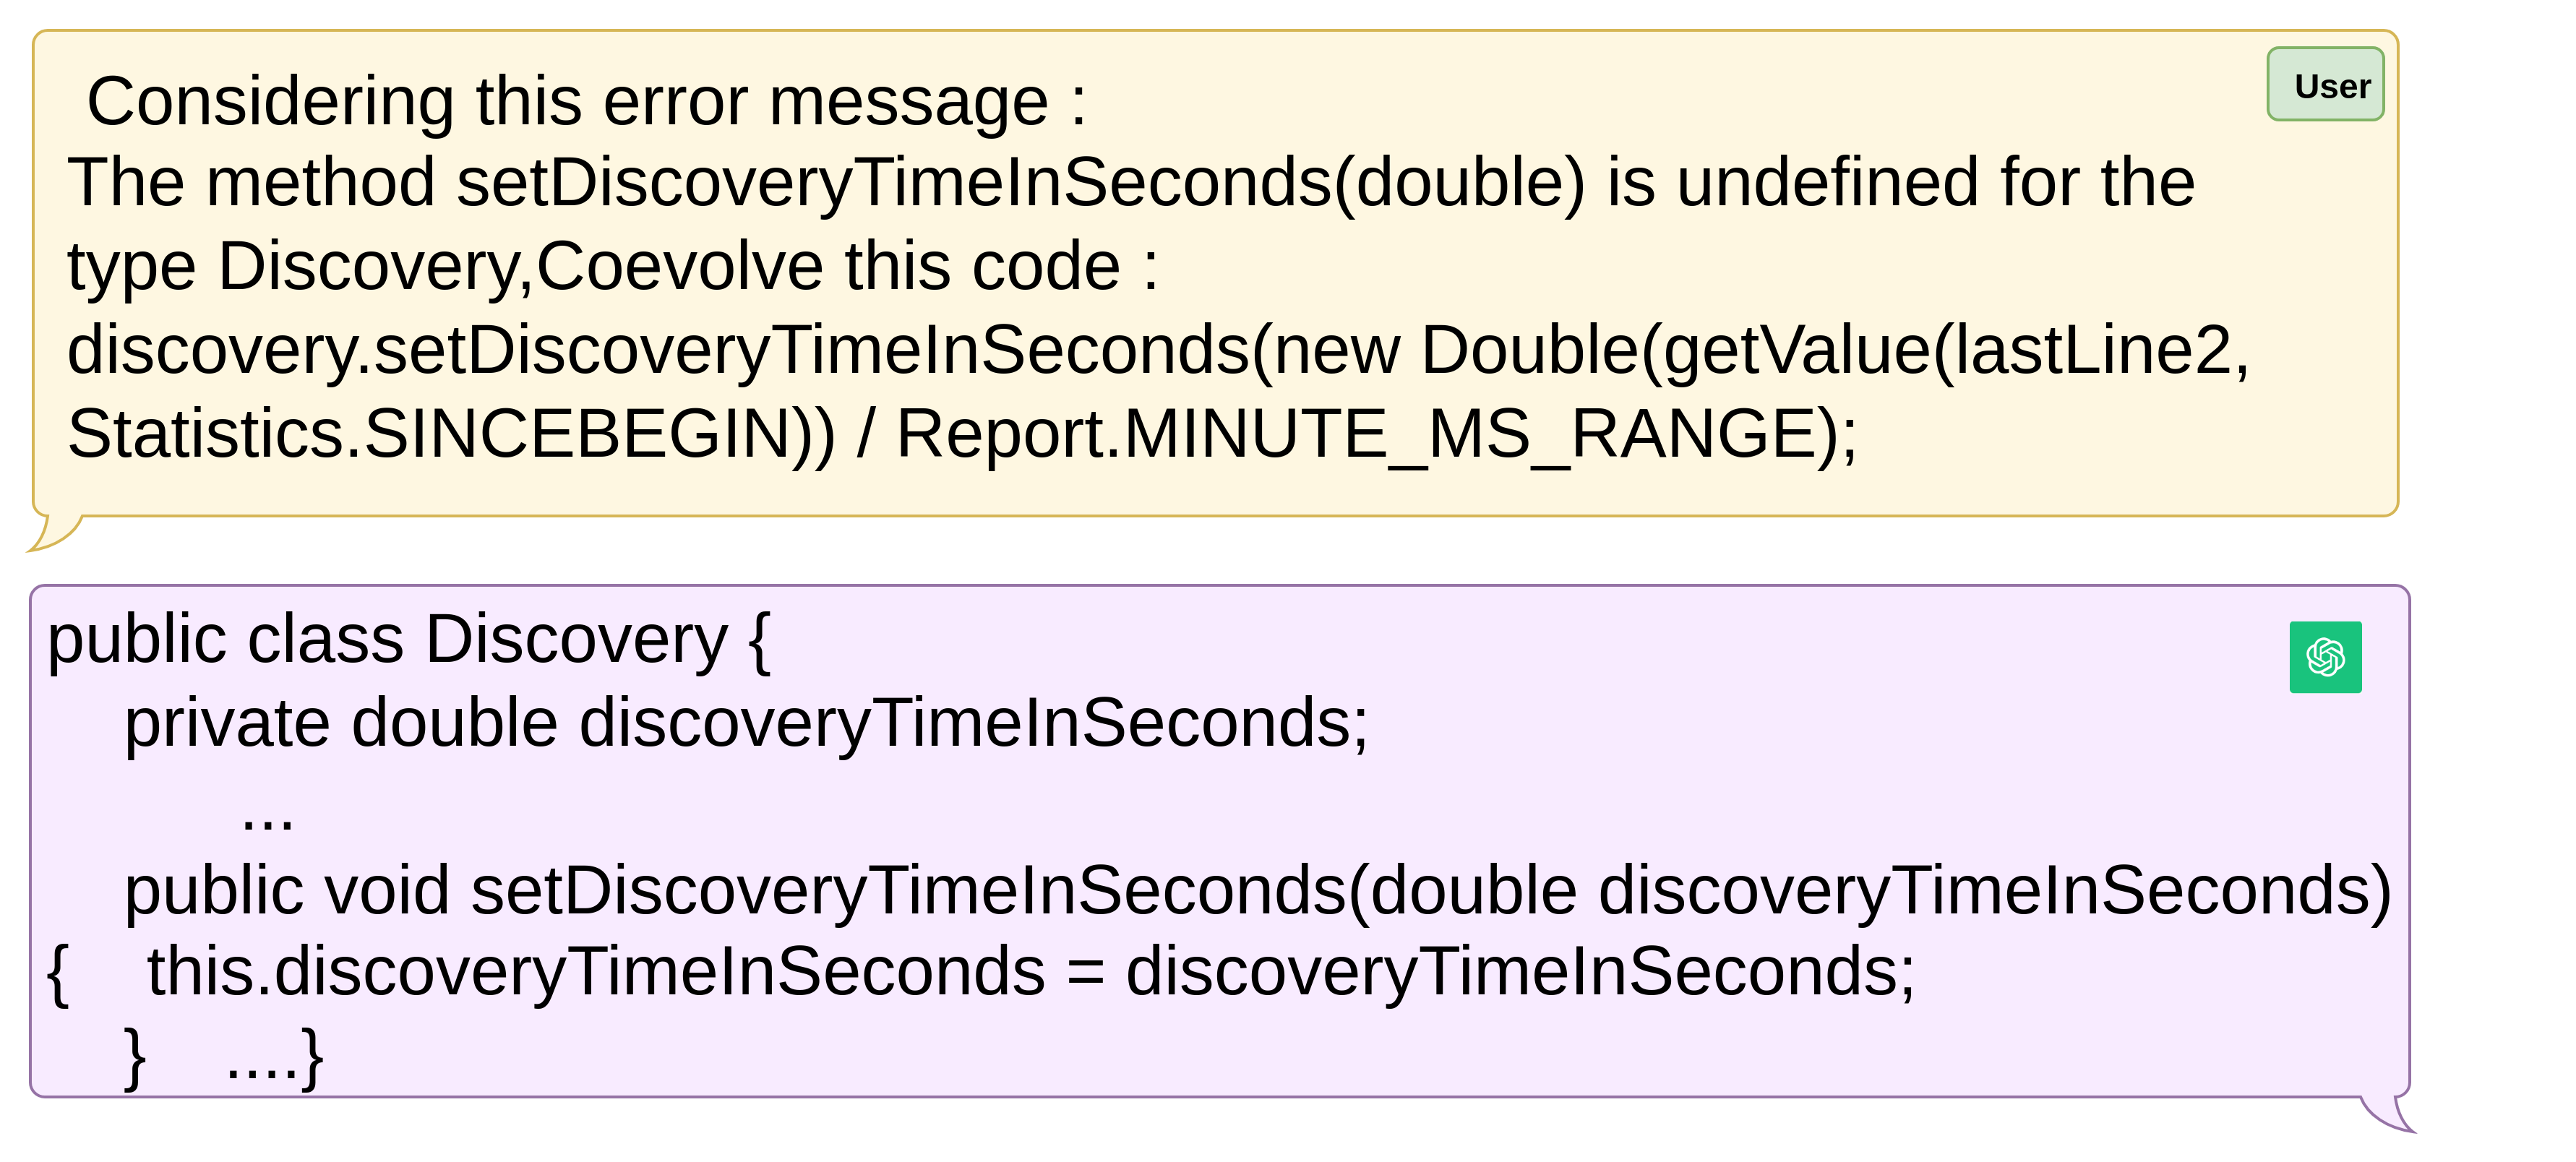
\includegraphics[width=0.48\textwidth]{./pics/chapter3pics/chatgptprimitiveanswer.png}
	\caption{ChatGPT primitive answer to the naive prompt.}
	\label{fig: chatgptanswer}
	%\vspace{-5mm}
\end{figure}

\begin{figure}[t]
	\centering
	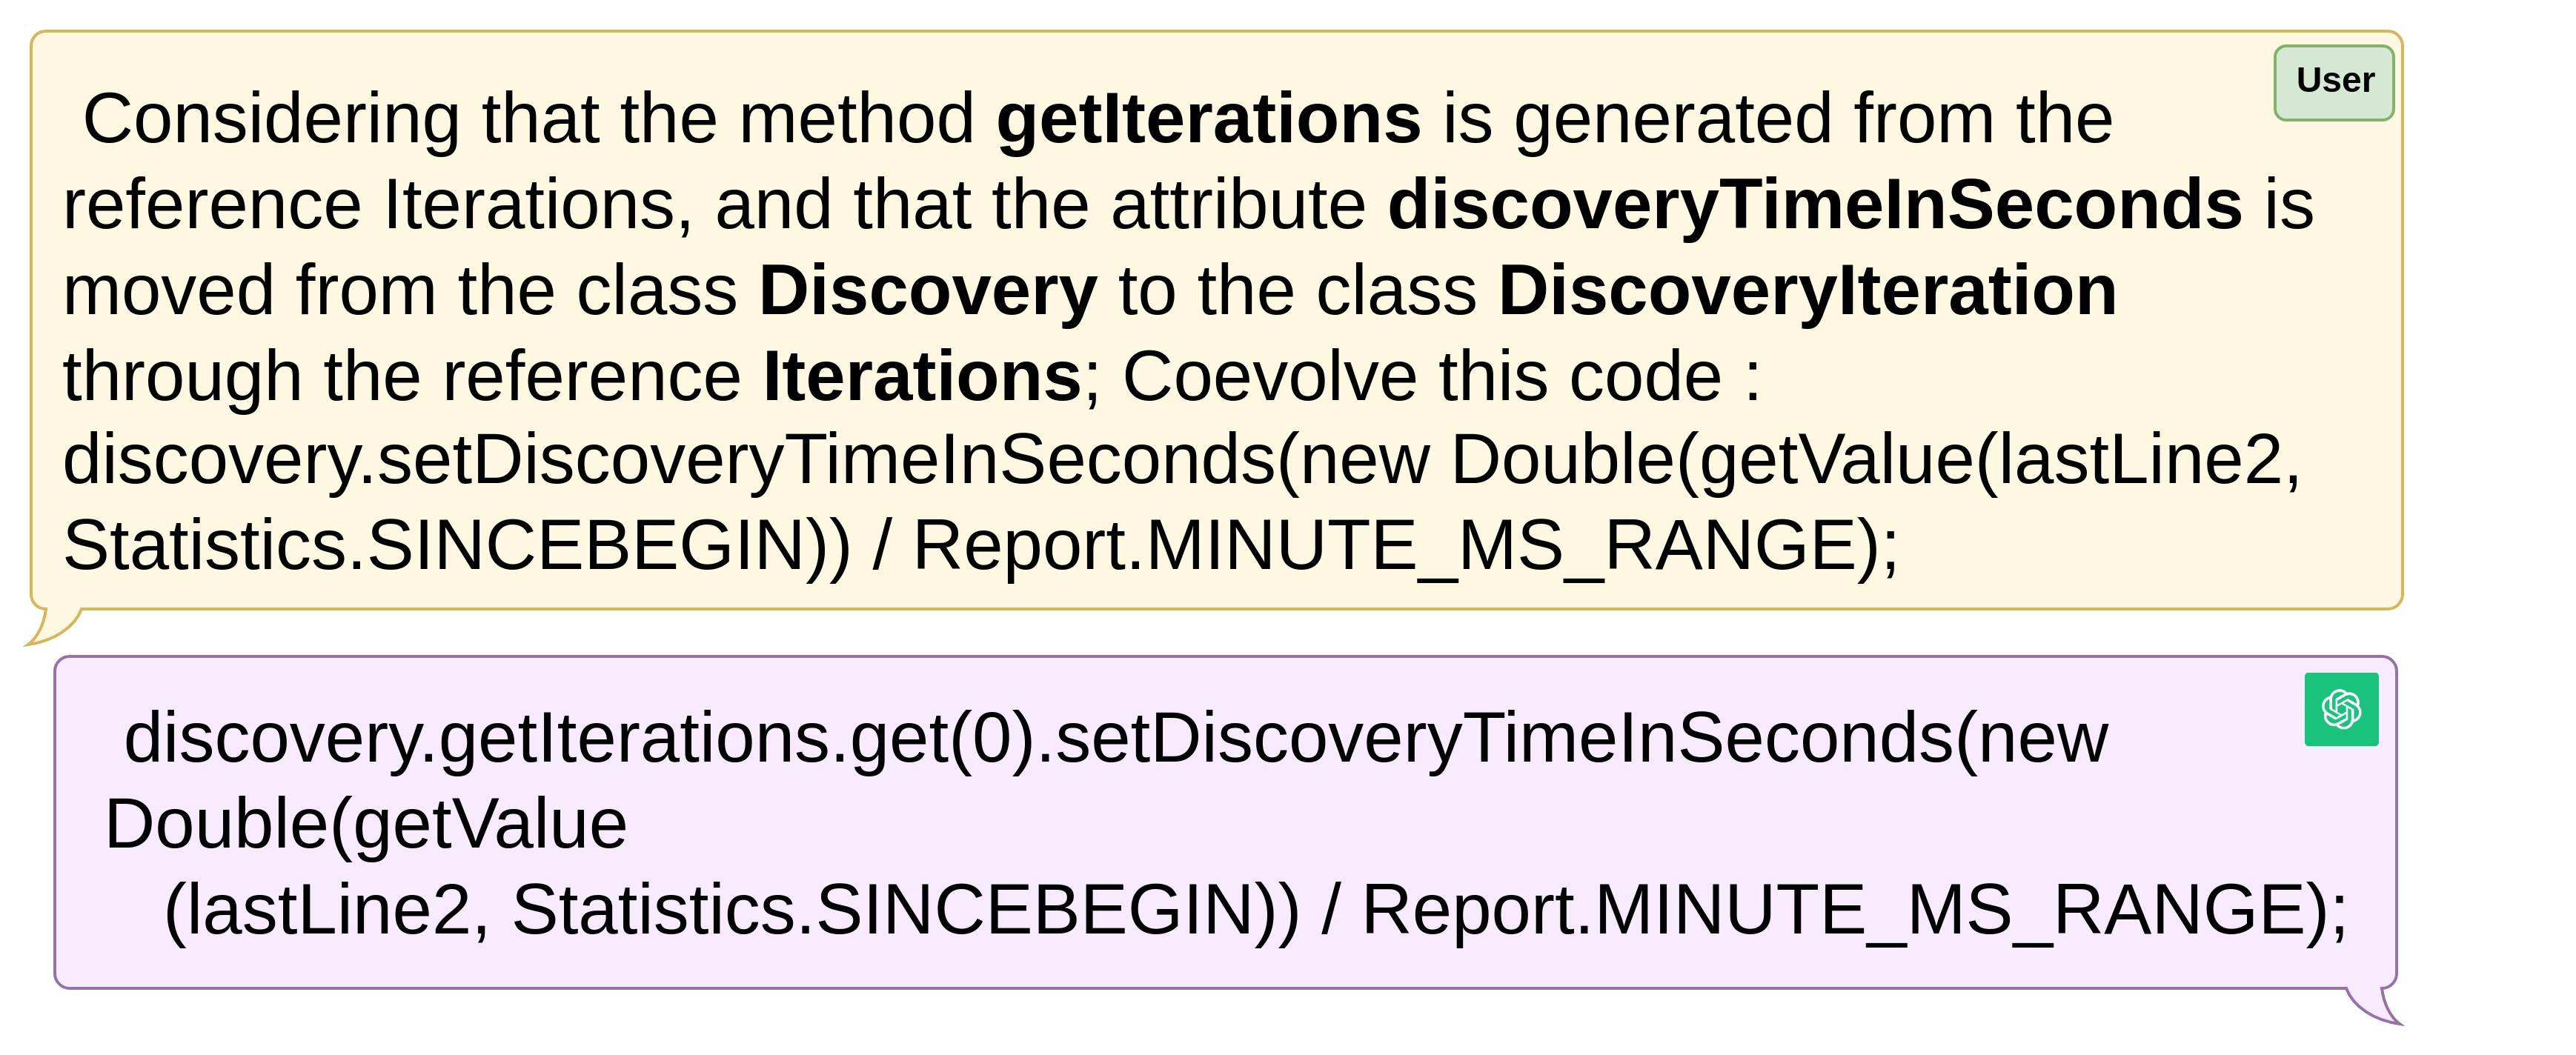
\includegraphics[width=0.48\textwidth]{./pics/chapter3pics/chatgptimprivedanswer.png}
	\caption{\LLM improved answer with the enriched prompt with contextual information.}
	\label{fig: chatgptimprovedanswer}
	\vspace{-5mm}
\end{figure}
\section{Prompt-Based Approach}
\label{appraoch}
This section introduces our approach to generate the prompts needed for the code co-evolution. 
It first gives an overview of the approach. Then details the structure of the generated prompts, before to detail each part of it and how it is generated. Finally, it describes our prototype implementation.  

\begin{figure}
	\centering
	\hspace*{-0.8cm}
	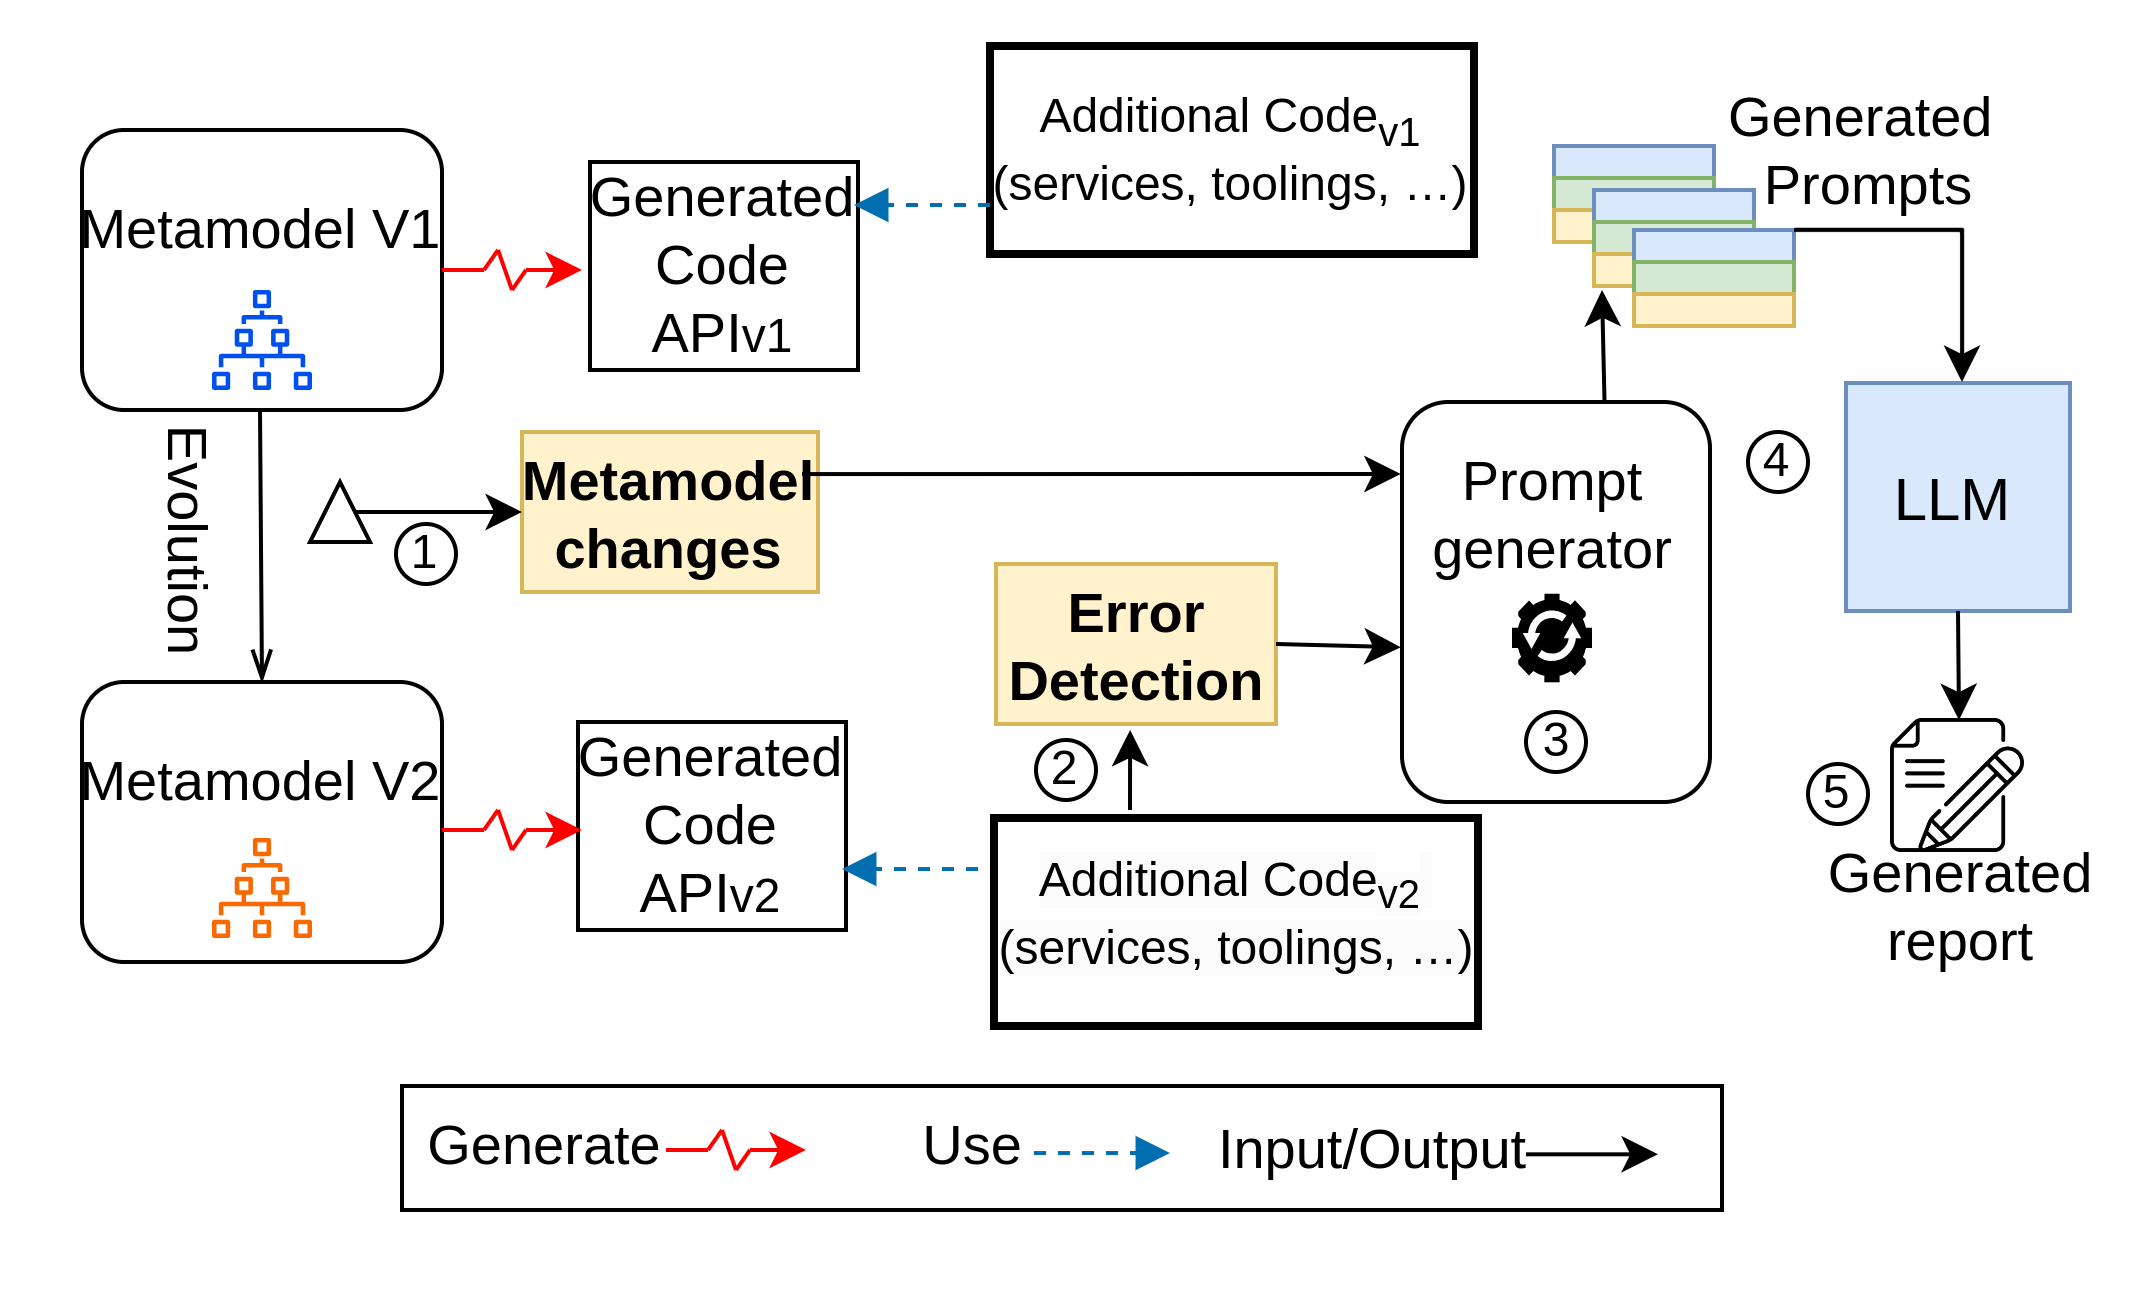
\includegraphics[width=0.55\textwidth]{./pics/chapter3pics/approach.png}
	\caption{Overall Approach for Prompt-based co-evolution.}
	\label{fig: approach}
	%\vspace{-5mm}
\end{figure}



\subsection{Overview}

Figure \ref{fig: approach} shows the overall steps of our approach. We start by retrieving the list of changes that describe the evolution between the old metamodel and the new metamodel~\Circled{1}. 

When the metamodel evolves, the code API is regenerated, therefore the additional code is broken. The additional code is then parsed to collect the list of errors~\Circled{2}. The list of changes and the list of errors are the inputs of our prompt generator. The goal is to generate a prompt for each error, including sufficient information about the change and the error itself~\Circled{3}.
Each generated prompt is used to request ChatGPT to give a correction for the concerned error~\Circled{4}. A global report is generated for the additional code to allow the developer to have a visual output about the generated prompts and the answers of the LLM~\Circled{5}. Algorithm \ref{algo:overallalgo} further depicts the overall method of co-evolution based on a given LLM. After we parse the project, we retrieve the list of errors per class (Lines 2-3). Then for each error, we generate the prompt (Lines 4-5) and call the LLM and record its co-evolution response for analysis (Lines 6-7).
%\Circled{1}


\begin{algorithm2e}[t]
	% \algsetup{linenosize=\tiny}
	\small
	\SetAlgoLined
	\KwData{EcoreModelingProject, changesList}
	javaClasses $\leftarrow$ Parse(EcoreModelingProject)
	
	\For {( jc $\in$ javaClasses)}
	{
		errorsList $\leftarrow $ getErrors(jc)
		
		\For{(error : errorsList)}
		{
			prompt $\leftarrow$ promptGenerator(error, changesList, jc)
			
			coevolutionResponse $\leftarrow$ callLLM(prompt)
			
			addToReport(error, prompt, coevolutionResponse)
		}
	}
	
	
	\caption{\LLM Co-evolution}
	\label{algo:overallalgo}
\end{algorithm2e}

\subsection{Generated Prompt Structure}

\begin{figure}[t]
	\centering
	%\hspace*{-1cm}
	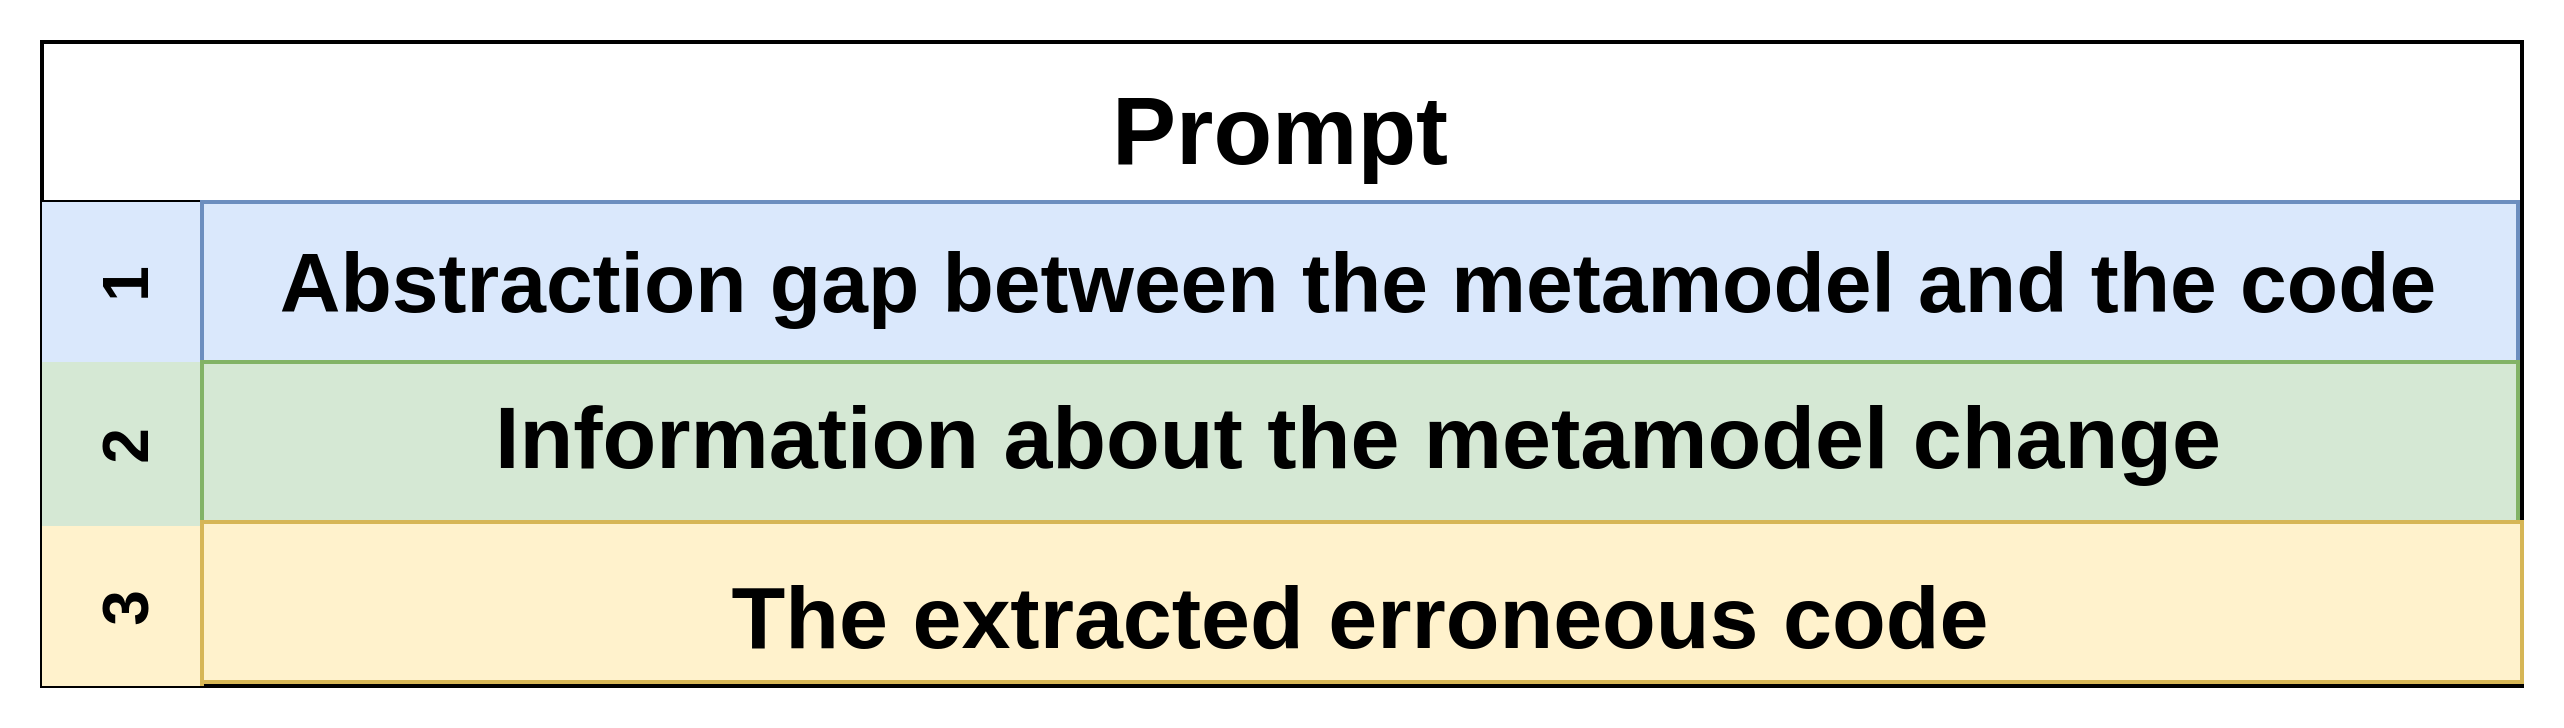
\includegraphics[width=0.5\textwidth]{./pics/chapter3pics/promptTemplate.png}
	\caption{Generated Prompt Structure.}
	\label{fig:promptstructure}
	\vspace{-5mm}
\end{figure}

Figure \ref{fig:promptstructure} shows the overall structure of the envisioned prompts we will generate in order to co-evolve the code errors. In fact, the rationale behind the prompt structure is that our problem does not only concern the code errors to repair, but it is also related to the use of the code generated from the metamodels and their changes. Therefore, to contextualize our problem, we must explain :~1) what is the code generated from the metamodels,~2) what is the impacting metamodel change, and~3) what is the impacted code error to co-evolve.  Concerning the prompt prefix we use "Co-evolve this code" to ask \LLM for one co-evolution. Next subsections detail the different parts of the prompt structure. 

\subsection{Abstraction Gap Between Metamodels and Code}

One main distinction from simply repairing code errors is the interplay between the metamodels and the additional code through the generated code from the metamodels. This is due to the gap in abstraction in between metamodels and generated code. In fact, for each metamodel various code elements are generated for each metamodel element and with different patterns.
Table~\ref{table:locationofMMelemen} classifies and provides illustrative examples for the different generated code elements from each metamodel element, namely metaclass, attribute/reference, and method.  %It shows that various code elements are generated for each metamodel element type and with different patterns. 
%%mapping between the different metamodel elements and their corresponding generated code elements with illustrative examples. 
For example, take the case of a metaclass\footnote{For simplicity, we refer to a metaclass by simply a class in the remaining of the paper.}. EMF generates a corresponding interface and a class implementation, a \emph{createClass()} method in the factory class, three literals (\ie constants) for the class and an accessor method in the package class, and a corresponding to create adapter method. For the attribute case, EMF generates the signature and implementation of a getter and a setter, an accessor, and a literal. 
%This classification is essential to match the different errors with their corresponding pattern usages in the code, before to co-evolve them with the appropriate resolution strategy. 
This classification is essential to match the different errors with the right used generated code elements to explicit the abstraction gap. \red{If a class is changed, all its generated elements are impacted and their usages will be erroneous. For example, if a class is renamed, every invocation of the method "get+className" will be erroneous and must be co-evolved}. Thus, we consider the abstraction gap as the first contextual information we inject in the prompts for the LLM to co-evolve the code errors. 


\begin{table*}[t]

\caption{Classification of the different patterns of the generated code element from the metamodel elements. \\\hspace{3em} [Examples illustrated for a metaclass \emph{Rule}, property \emph{Status}, and method \emph{Execute()}]} 

\label{table:locationofMMelemen}
	\resizebox{17cm}{!} {
{\small
\begin{tabular}{llll}
\toprule

\begin{tabular}[c]{@{}l@{}} \textbf{Metamodel}\\ \textbf{element type} 
\end{tabular} & \textbf{Generated code elements}& \textbf{Pattern of the generated code elements}& \textbf{Examples}\\ \midrule


\multirow{6}{*}{Metaclass} & Interface & "MetaClassName" & \textit{Rule} \\ \cline{2-4} 
 & \begin{tabular}[c]{@{}l@{}}createClass() \\ (in metamodelFactory class)\end{tabular} & "create"+"MetaClassName"() &\textit{createRule()} \\ \cmidrule{2-4} 
 & \begin{tabular}[c]{@{}l@{}}Literals of the class \end{tabular} &
 \begin{tabular}[c]{@{}l@{}}
 "META\_CLASS\_NAME"\\
 "META\_CLASS\_NAME"+"\_"+ "FEATURE\_COUNT"\\
 "META\_CLASS\_NAME"+ "\_"+"OPERATION\_COUNT"
 \end{tabular} 
 & \begin{tabular}[c]{@{}l@{}}\textit{RULE}, \\ \textit{RULE\_FEATURE\_COUNT}, \\  \textit{RULE\_OPERATION\_COUNT}\end{tabular} \\ \cmidrule{2-4} 
 & \begin{tabular}[c]{@{}l@{}}Accessor of Meta objects \\ (in metamodelPackage class)\end{tabular} & "get"+"MetaClassName"()& \textit{getRule() }\\ \cmidrule{2-4} 
 & Class implementation & "MetaClassNameImpl" &\textit{RuleImpl }\\ \cmidrule{2-4} 
 & Adapter & "create"+"MetaClassName"+"Adapter" & \textit{createRuleAdapter()} \\ \midrule


\multirow{1}{*}{Attribute} & Signature of getters and setters & "get"+"AttributeName"(), "set"+"AttributeName"()& \textit{getStatus()}, \textit{setStatus() }\\ \cmidrule{2-4} 
\multirow{2}{*}{(Same for a} & Accessor of Meta objects &"get"+"MetaClassName"+"\_"+"AttributeName"() &\textit{getRule\_Status()} \\ \cmidrule{2-4} 
\multirow{1}{*}{Reference)}  & Literal & "META\_CLASS\_NAME"+"\_\_"+"ATTRIBUTE\_NAME"& \textit{RULE\_\_STATUS} \\ \cmidrule{2-4} 
 & \begin{tabular}[c]{@{}l@{}}Implementation \\ of getters and setters\end{tabular} &"get"+"AttributeName"(), "set"+"AttributeName"()& getStatus(), setStatus() \\ \midrule


\multirow{4}{*}{Method} & Declaration of the method& "methodName"()& \textit{Execute() }\\ \cmidrule{2-4} 
 & Accessor of meta objects &"get"+"MetaClass"+"\_\_"+"MethodName"()& \textit{getRule\_\_Execute() }\\ \cmidrule{2-4} 
 & Literal &"META\_CLASS\_NAME"+"\_\_"+"METHOD\_NAME"& \textit{RULE\_\_\_EXECUTE}\\ \cmidrule{2-4} 
 & Implementation of the method &"methodName"()& \textit{Execute()} \\ %\midrule


%\multirow{4}{*}{Reference} & Accessor of meta objects &"get"+"MetaClassName"+"\_"+"ReferenceName"()& \textit{getConstraint\_ConstraintElement()} \\ \cmidrule{2-4} 
% & Signature of getters and setter & "get"+"ReferenceName"(),"set"+"ReferenceName"()&\textit{ getConstraintElement()}, \textit{setConstraintElement() }\\ \cmidrule{2-4} 
% & Literal &"META\_CLASS\_NAME"+"\_\_"+"REFERENCE\_NAME"& \textit{CONSTRAINT\_\_CONSTRAINT\_ELEMENT} \\ \cmidrule{2-4} 
% & \begin{tabular}[c]{@{}l@{}}Implementation of \\ getters and setters\end{tabular} &"get"+"ReferenceName"(), "set"+"RegerenceName"()& \textit{getConstraintElement()}, \textit{setConstrainElement() }\\ 
\bottomrule
 
 %cline hline replaced with cmidrule and midrule
 
\end{tabular}
}
}
\end{table*}



\subsection{Metamodel Evolution Changes}
\label{mmchanges}
A metamodel represents a high abstraction level of a domain.
Like any software artefact, metamodels evolve to meet domain changing requirements \cite{mens2008introduction}.
Herrmannsdoerfer et al. \cite{Herrmannsdoerfer2011} distinguish two types of metamodel changes: \emph{atomic} and \emph{complex}. Atomic changes are additions, removals, and updates of a metamodel element. Complex changes consist of a combination of atomic changes ~\cite{vermolen2011reconstructing,khelladi2015detecting}. 
%
For example, push property is a complex change where a property is pushed from a parent class to an inheriting child class. This is composed of two atomic changes: delete a property and add a property~\cite{Herrmannsdoerfer2011}. 
Many approaches in the literature~\cite{Alter2015, williams2012searching,cicchetti2009managing,langer2013posteriori,vermolen2011reconstructing,Khelladi2016,bettini2022executable} exist to detect metamodel changes between two versions. 
\red{Particularly in our work, we use \cite{Khelladi2016,khelladi2016ad} to extract the changes between two metamodel versions. }

In practice, we focus on the impacting metamodel changes that will require co-evolution of the code and not on the non-impacting changes. For example, an add change of a class does not require co-evolution. However, a delete change or a change of type will impact the code that must be co-evolved. 
%Table \ref{xyz} gives 
The list of impacting metamodel changes \cite{iovino2012impact,cicchetti2009managing} we consider in the prompts is as follows: \emph{1)} Delete property\footnote{Property refers to Attribute, Reference, and Method.} \emph{p} in a class \texttt{C}, \emph{2)} Delete class \texttt{C}, \emph{3)} Rename element \emph{e} in a class \texttt{C}, \emph{4)} Generalize property \emph{p} multiplicity from a single value to multiple values in a class \texttt{C},  \emph{5)} Move property \emph{p} from class \texttt{Source} to \texttt{Target} through a reference \emph{ref},  \emph{6)} Extract class of properties $p_{1},...,p_{n}$ from \texttt{Source} to \texttt{Target} through a reference \emph{ref},  \emph{7)} Push property \emph{p} from super class \texttt{Super} to sub classes \texttt{Sub$_{1}$},...,\texttt{Sub$_{n}$}, \emph{8)} Inline class \texttt{Source} to \texttt{Target} with properties $p_{1},...,p_{n}$, and \emph{9)} Change property \emph{p} type from \texttt{S} to \texttt{T} in a class \texttt{C}. 

\begin{comment}
	\item \emph{1)} Delete property\footnote{Property refers to Attribute, Reference, and Method.} \emph{p} in a class \texttt{C}. 
	
	\item \emph{2)} Delete class \texttt{C}. 
	
	\item \emph{3)} Rename element \emph{e} in a class \texttt{C}. 
	
	\item \emph{4)} Generalize property \emph{p} multiplicity from a single value to multiple values in a class \texttt{C}. 
	
	\item \emph{5)} Move property \emph{p} from class \texttt{Source} to \texttt{Target} through a reference \emph{ref}. 
	
	\item \emph{6)} Extract class of properties $p_{1},...,p_{n}$ from \texttt{Source} to \texttt{Target} through a reference \emph{ref}. 
	
	\item \emph{7)} Push property \emph{p} from super class \texttt{Super} to sub classes \texttt{Sub$_{1}$},...,\texttt{Sub$_{n}$}. 
	
	\item \emph{8)} Inline class \texttt{Source} to \texttt{Target} with properties $p_{1},...,p_{n}$. 
	
	\item \emph{9)} Change property \emph{p} type from \texttt{S} to \texttt{T} in a class \texttt{C}. 
\end{comment}

Thus, we consider these definitions of metamodel changes as the second contextual information we inject in the prompts for the LLM to co-evolve the code errors. 

%\emph{1)} Delete property \emph{p} in a class \texttt{C}. \emph{2)} Delete class \texttt{C}.\emph{3)} Rename element \emph{e} in a class \texttt{C}. \emph{4)} Generalize property \emph{p} multiplicity from a single value to multiple values in a class \texttt{C}. \emph{5)} Move property \emph{p} from class \texttt{S} to \texttt{T} through a reference \emph{ref}. \emph{6)} Extract class of properties $p_{1},...,p_{n}$ from \texttt{S} to \texttt{T} through a reference \emph{ref}. \emph{7)} Push property \emph{p} from super class \texttt{Sup} to sub classes \texttt{Sub$_{1}$},...,\texttt{Sub$_{n}$}. \emph{8)} Inline class \texttt{S} to \texttt{T} with properties $p_{1},...,p_{n}$. \emph{9)} Change property \emph{p} type from \texttt{S} to \texttt{T} in a class \texttt{C}.


\subsection{Extracted Code Errors}

Now that we have two main ingredients needed for the generation of the prompts. %, namely metamodel changes and the abstraction gap between metamodels and code. 
We only require the erroneous code to be co-evolved. 

To do so, we parse the code (i.e., \emph{compilation units}) to access the Abstract Syntax Trees (ASTs) and retrieve the code errors. %An error in a Java code is called a \emph{Marker} that contains the information regarding the detected error. It
Each error contains the necessary information to locate the exact impacted AST node in the parsed global AST (\ie char start and end) and to process it (\ie message). 
After that, we simply extract the sub-AST corresponding to the code containing the error. 
We consider three possible situations, namely 1) if the error is in a method, we extract the whole method, 2) if the error is in the imports, we extract the list of imports, 3) if the error is in the class definition or the fields, we extract it without the class's methods. This constitutes the final part of the contextual information we inject in the prompts for the LLM to co-evolve the code errors. Note that we simply specify in the prompt before the code the order to \emph{"Co-evolve this code: "}.
%\red{This prefix is selected after trying other terms like "update" and "correct" because it is more related to our problem.}.

%In the remaining part of the paper, we refer to errors and Java classes for the sake of simplicity. 


%\begin{figure}[t]\centering%
%\scalebox{0.9}{\small\input{pics/PromptStructure}}
% \vspace*{-0.3cm}
%\caption{Generated Prompt Structure.}
%\label{fig:promptStruct}
%\vspace{-1em}
%\end{figure}

\subsection{Prompt Generation}
\label{promptgeneration}

Algorithm~\ref{algo:promptgenerator} allows generating prompts following the specified structure in Figure~\ref{fig:promptstructure}. It first finds the ASTNode corresponding to the error in the code (Line~1). Then, it iterates over the list of metamodel changes to match  the error node with the code usage to identify the impacted abstraction gap (Lines~6-8). After that, it summarizes the impacting metamodel change (Line~11). Finally, it extracts the erroneous code (Line~21) and puts together all three contextual information into one generated prompt (Lines~22-25). 
%
Figure~\ref{fig:promptexample} shows an example of the generated prompt for the error in Listing~\ref{lis:Modisco_Code_External_V1} (Line~4) due to the move of property \emph{DiscoveryTimeInSeconds} in the metamodel.  

\begin{figure}[t]
	\centering
	%\hspace*{-1cm}
	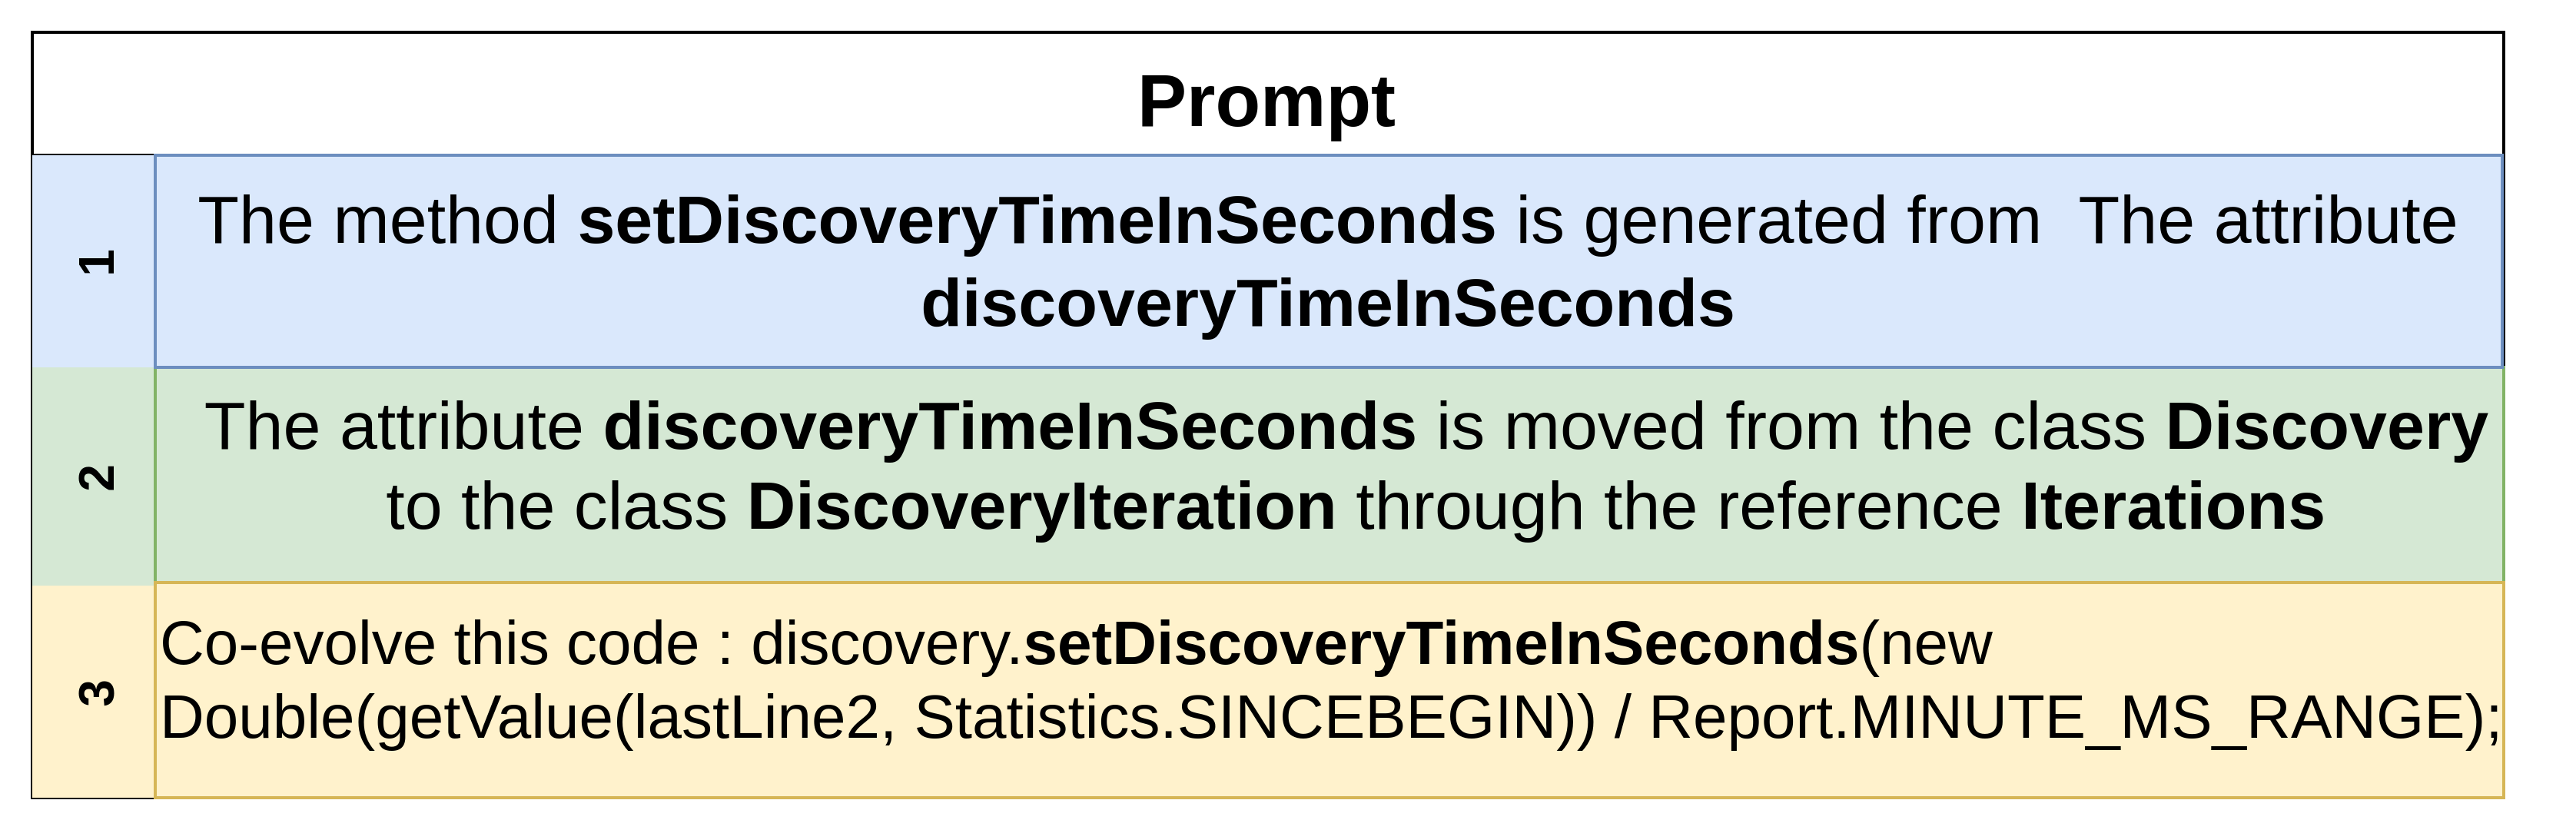
\includegraphics[width=0.5\textwidth]{./pics/chapter3pics/PromptStructure.png}
	\caption{Move attribute prompt example.}
	\label{fig:promptexample}
	\vspace{-5mm}
\end{figure}


\begin{algorithm2e}[t]
	% \algsetup{linenosize=\tiny}
	\small
	\SetAlgoLined
	\KwData{error, changesList, javaClass}
	
	errorNode $\leftarrow$ findErrorAstNode(javaClass, error)
	
	found $\leftarrow$ false
	
	%\uIf{(errornode.isTypeOf( SimpleName))}
	%{
		\While {(change  $\in$ changesList $\&$ $\neg found$)}
		{
			\Switch{change}{
				\Case{RenameClass}{%V errornode.name="set"+change.name)
					\uIf{(errornode.name="get"+change.name )}
					{
						found $\leftarrow$ true  
						
						abstractionGap="The method "+ errornode.name+" is generated from the metaclass "+ change.name
					} 
					\uElseIf {...}{\emph{\textcolor{circlegreen}{/*treat other abstraction gaps*/}}}
					changeInfo= "The metaclass "+ change.oldName+" is renamed to "+change.newName
				}
				\Case{RenameProperty}{
					...
				}
				\Case{DeleteProperty}{
					...
				}
			}
			
			
		}
		%} \uElseIf {( errornode.isTypeOf( QualifiedName))}
	%{	  \emph{\textcolor{circlegreen}{/*repeat same matching process*/}}
		%...
		%}
	
	
	codeError $\leftarrow$ extractCodeError(errornode)
	
	prompt.add(abstractionGap)
	
	prompt.add(changeInfo)
	
	prompt.add(codeError) 
	
	\textbf{return} prompt
	
	\caption{Prompt Generator Algorithm}
	\label{algo:promptgenerator}
\end{algorithm2e}


\begin{comment}
	
	
	\begin{algorithm2e}[t]
		% \algsetup{linenosize=\tiny}
		\small
		\SetAlgoLined
		\KwData{error, changesList, javaClass}
		
		errorNode $\leftarrow$ findErrorAstNode(javaClass, error)
		
		\uIf{(errornode.isTypeOf( SimpleName))}
		{
			\For {(change  $\in$ changesList)}
			{
				\Switch{change}{
					\Case{RenameClass}{%V errornode.name="set"+change.name)
						\uIf{(errornode.name="get"+change.name )}
						{
							request="The method "+ errornode.name+" is generated from the metaclass "+ change.name
							+" That is renamed from " +change.name+ " to "+change.newName
						}   
					}
					\Case{RenameProperty}{
						...
					}
					\Case{DeleteProperty}{
						...
					}
				}
			}
		} \uElseIf {( errornode.isTypeOf( QualifiedName))}
		{	  \emph{\textcolor{circlegreen}{/*repeat same matching process*/}}
			...
		}
		code$\leftarrow$getCode(errornode)
		
		prompt.add(request)
		
		prompt.add(code)
		
		\textbf{return} prompt
		\caption{Prompt generator algo}
		\label{algo:promptgenerator}
	\end{algorithm2e}
	
	
\end{comment}



%\subsection{Prototype Implementation}

\subsection{Prototype Implementation}
We implemented our solution as an eclipse Java plugin handling Ecore/EMF metamodels and their Java code. To retrieve the list of errors, we used JDT eclipse plugin \footnote{Eclipse Java development tools (JDT): \url{https://www.eclipse.org/jdt/core/}}. To launch our tool, we added a command to the context menu when selecting a java project. Generated prompts are sent to \LLM (see next section \ref{selectedLLM}), more specifically, its OpenAI API endpoint "https://api.openai.com/v1/chat/completions". We used Java JSON package to send our prompts and to receive \LLM responses. The error location, the corresponding generated prompt and \LLM responses are parsed in CSV file to have a visible results and to keep the history of proposed the co-evolutions.
Moreover, quick fixes (our baseline) are called using 
\textit{org.eclipse.jdt.ui.text.java.IQuickAssistProcessor} and \textit{org.eclipse.jdt.ui.text.java.IJavaCompletionProposal}.

\section{Methodology}
\label{evaluation}

This section describes our methodology for empirically assessing the capabilities of \LLM in addressing the problem of metamodel and code co-evolution. 
It first describes the selected LLM and the followed evaluation process.
Then, it presents our research questions and the data set.

\subsection{Selected LLM}\label{selectedLLM}
%\red(GPT-3.5, 4.0 ?)
% Motivate the use of chatgpt
% Motivate the use of gpt-3.5-turbo, chat mode

We chose to use \LLM \emph{GPT-3.5-turbo} in chat mode. It currently points to \emph{gpt-3.5-turbo-0613} released in June 2023. We opted for this model because of four factors. The first one is that prompt content is only textual, we don't need to inject audio or image content. The second one is its capacity to generate good answers for requests about code and models generation \cite{nathalia2023artificial,yeticstiren2023evaluating,guo2023exploring,fu2023chatgpt,kabir2023empirical,chaaben2023towards,camara2023assessment}. The third factor is that it was the latest API version that is accessible, \emph{gpt-4} API still not accessible for us. The last one is related to the high popularity of \LLM as a tool. It has more than 100 million users, and its website saw more than 1.7 billion visitors in the last three months, with Software and Software Development as visitors' top category\footnote{\url{https://www.similarweb.com/fr/website/chat.openai.com/\#demographics}}. 


\subsection{Evaluation Process}


First, as we aim to query \LLM to co-evolve the erroneous code due to metamodel evolution, we need to provoke the errors in the code. To do so, we replace the original metamodel by the evolved metamodel. Then, we regenerate the code API with EMF. This will cause errors in the additional code that must co-evolve. 
%
After that, we must map the errors with the causing metamodel change before to generate a prompt with all appropriate information to be able to co-evolve the code errors. We then rely on the OpenAI API to query \LLM before to analyze its results. 
%
%\todo{explain how we measure correctness ?}
%
Finally, we measure the correctness of \LLM co-evolution by comparing its co-evolution with the manually co-evolved version by developers. \red{Note that the comparison is processed manually by authors}. This allows us to measure the \emph{correctness} reached by \LLM. %We distinguish between \emph{syntactically} and \emph{semantically} correct co-evolution. The former is when \LLM gives the exact expected co-evolution that is also , whereas the latter is syntactically different but behave the same as the expected co-evolution, hence, semantically correct. 
%We consider a solution to be correct if it matches 
Correctness varies from~0 to~1, i.e., 0\% to 100\% and is defined as follows:
%alternative to terminology of syntactically, semantically
\vspace{0.5em}

\noindent $ Correctness = \dfrac{LLM Coevolutions \cap Manual Coevolutions}{Manual Coevolutions} $

\vspace{0.5em}

We chose the structure shown in Figure \ref{fig:promptstructure} since it contains the contextual information needed for our problem of metamodels and code co-evolution. \red{This structure was built after few manual naive attempts with \LLM, starting from a minimum context (as shown in the Motivating Example of Figure~\ref{fig: chatgptanswer} that failed) and by enriching the structure with more context information}. However, we do not claim its completeness in terms of needed information or if it is the best structure. Other variants can lead to different results. 
%for generated prompts after several manual attempts with Chatgpt. 
To investigate more this choice, we generated three more variations of this structure to observe its effect on the results. Table \ref{table: op variations} contains each variation and its corresponding explanation. Since our prompt contains three parts, we can change the order of these parts (Order Change operator) and the size of the erroneous code we put in the prompt (Minimal Code operator). Finally, rather than asking for a single co-evolution solution, we ask for alternative ones (Alternative Answers operator) in the prompt prefix. \red{To stress out our evaluation, we conducted 5 runs separated by almost a day, the time we needed for one run to check manually the results of each project, which means that each generated prompt is proposed to \LLM five times. This aims to check whether \LLM gives a same or different answer, hence, assess its robustness. 
	Finally, we compare \LLM to a baseline, namely the IDE quick fixes that are provided to repair the code errors. Note that we do not take as a baseline \LLM with prompts that only contain the code error, since as shown in Section \ref{example} and Figure \ref{fig: chatgptanswer}, it does not work. 
}


\subsection{Research Questions}

To assess the capabilities of \LLM in the co-evolution of code, we set the following research questions. 

\begin{itemize}
	\item[RQ1] %\subsubsection{RQ1} 
	%Can our code and metamodel coevolution appraoch using LLMs coevolve the code correctly? 
	To what extent can \LLM co-evolve the code with evolved metamodels? 
	This aims to assess the ability of \LLM to give correct resolutions to co-evolve the code according to the metamodel changes.
	
	\item[RQ2] %\subsubsection{RQ2}
	How does varying the temperature hyperparameter affect the output of the co-evolution? %How does our coevolution approach react to the variation of the prompt? 
	The temperature hyperparameter controls the creativity of the language model. 
	This question aims to assess the capability of \LLM to co-evolve the erroneous code when given less or more creativity in the generation of the solution. 
	
	
	\item[RQ3] %\subsubsection{RQ2}
	How does varying the prompt structure affect the output of the co-evolution? %How does our coevolution approach react to the variation of the prompt? 
	This aims to assess the quality improvement of the co-evolutions due to the prompts' variations.
	
	
	\item[RQ4] %\subsubsection{RQ3} 
	How does \LLM proposed co-evolution compare to the quick fix baseline? 
	As quick fixes are provided by default in an IDE to repair the code errors, this question aims to assess which method outperforms the other in the task of code co-evolution with evolving metamodels. %We measure its precision and recall and compare it with precision and recall of our automatic co-evolution approach.
	
	
\end{itemize}



\begin{table*}[t]
	\centering
	\caption{Variation operators of our original prompt (OP).}
	\label{table: op variations}
	\resizebox{14cm}{!} {
		\begin{tabular}{ll}
			\toprule
			Variation Operators       & Explanation                               \\ \midrule
			Order Change (OC)         & \begin{tabular}[c]{@{}l@{}}We change the order between the three structured parts of the prompt. \\  We start by describing  the metamodel change before the abstraction gap.\end{tabular} \\ \midrule
			Minimal Code (MC)         & \begin{tabular}[c]{@{}l@{}}Instead of giving the whole method that contains the code error to co-evolve, \\ we only give the instruction of code error.\end{tabular}     \\ \midrule
			Alternative Answers (AA)  & \begin{tabular}[c]{@{}l@{}}Instead of asking the LLM to give one solution of co-evolution, \\ we specifically ask for alternative ways to co-evolve the code error.\end{tabular}           \\
			\bottomrule
			
		\end{tabular}
	}
\end{table*}


\begin{table*}[t]
	\centering
	\caption{Details of the metamodels and their evolutions.}
	\label{CaseStudies_Evolution}
	\resizebox{16.5cm}{!} {
		\begin{tabular}{cllll}
			\toprule
			Case study                                                                            & \begin{tabular}[c]{@{}l@{}}Evolved \\ metamodels\end{tabular}                 & Versions & 
			\multicolumn{1}{c}{\begin{tabular}[c]{@{}c@{}}Atomic changes \\in the metamodel\end{tabular}} & \multicolumn{1}{c}{\begin{tabular}[c]{@{}c@{}}Complex changes \\in the metamodel\end{tabular}} \\ \midrule		
			
			
			OCL & \begin{tabular}[c]{@{}l@{}}Pivot.ecore in project\\ocl.examples.pivot\end{tabular}                        &  \begin{tabular}[c]{@{}l@{}}3.2.2 to\\ 3.4.4\end{tabular}        &   
			\begin{tabular}[c]{@{}l@{}} Deletes: 2 classes, 16 properties, 6 super types \\ Renames: 1 class, 5 properties \\ Property changes: 4 types; 2 multiplicities \\ Adds: 25 classes, 121 properties, 36 super types  \end{tabular}                                                         &    \begin{tabular}[c]{@{}l@{}} 1 pull property \\ 2 push properties  \end{tabular}                                                        \\ \midrule 
			Modisco & \begin{tabular}[c]{@{}l@{}}Benchmark.ecore in project\\modisco.infra.discovery.benchmark\end{tabular}                & \begin{tabular}[c]{@{}l@{}}0.9.0 to\\ 0.13.0\end{tabular}         &     
			\begin{tabular}[c]{@{}l@{}} Deletes: 6 classes, 19 properties, 5 super types \\ Renames: 5 properties  \\ Adds: 7 classes, 24 properties, 4 super types  \end{tabular}                                                        &     \begin{tabular}[c]{@{}l@{}} 4 moves property \\ 6 pull property \\ 1 extract class \\ 1 extract super class \end{tabular}                                                       \\ \midrule		
			
			
			Papyrus & \begin{tabular}[c]{@{}l@{}}ExtendedTypes.ecore in project\\papyrus.infra.extendedtypes\end{tabular}            & \begin{tabular}[c]{@{}l@{}}0.9.0 to\\ 1.1.0\end{tabular}         &   
			\begin{tabular}[c]{@{}l@{}}Deletes: 10 properties, 2 super types \\ Renames: 3 classes, 2 properies \\ Adds: 8 classes, 9 properties, 8 super types  \end{tabular}                                                      &    \begin{tabular}[c]{@{}l@{}} 2 pull property \\ 1 push property \\ 1 extract super class \end{tabular} \\  \bottomrule 		
		\end{tabular}
	}
\end{table*}



\begin{table*}[t]
	\caption{Details of the projects and their caused errors by the metamodels' evolution.}
	\label{CaseStudies_CoEvolution}
	\resizebox{18.5cm}{!} {
		\begin{tabular}{llcccccc}
			\toprule
			\begin{tabular}[c]{@{}l@{}}Evolved \\ metamodels\end{tabular}                 & \begin{tabular}[c]{@{}l@{}}Projects to co-evolve in response to the \\ evolved metamodels \end{tabular} 	& \begin{tabular}[c]{@{}c@{}}$N^{o}$ of \\ packages\end{tabular} & \begin{tabular}[c]{@{}c@{}}$N^{o}$ of \\ classes\end{tabular} & 
			\begin{tabular}[c]{@{}c@{}}$N^{o}$ of \\ LOC\end{tabular} & \begin{tabular}[c]{@{}c@{}}$N^{o}$ of Impacted \\ classes\end{tabular} & \begin{tabular}[c]{@{}c@{}}$N^{o}$ of total \\ errors \end{tabular}\\ \midrule		
			
			\begin{tabular}[c]{@{}l@{}}OCL  Pivot.ecore\end{tabular}                     
			& \begin{tabular}[c]{@{}l@{}} $[P1]$ ocl.examples.xtext.base \\ \end{tabular}   
			&   \begin{tabular}[c]{@{}l@{}}12 \end{tabular}    
			& \begin{tabular}[c]{@{}l@{}}181 \end{tabular}                 
			& 	\begin{tabular}[c]{@{}l@{}}17599 \end{tabular} 
			& \begin{tabular}[c]{@{}l@{}} 10 \end{tabular} 
			& \begin{tabular}[c]{@{}l@{}} 29 \end{tabular}
			\\ \midrule	
			\begin{tabular}[c]{@{}l@{}}Modisco \\ Benchmark.ecore\end{tabular}            
			& \begin{tabular}[c]{@{}l@{}} $[P2]$ modisco.infra.discovery.benchmark\\ $[P3]$ gmt.modisco.java.discoverer.benchmark\\ $[P4]$ modisco.java.discoverer.benchmark\\ $[P5]$ modisco.java.discoverer.benchmark.javaBenchmark\end{tabular}  
			& \begin{tabular}[c]{@{}l@{}}3 \\8 \\10 \\3  \end{tabular}
			& \begin{tabular}[c]{@{}l@{}}28 \\21 \\28 \\16 \end{tabular} 
			& \begin{tabular}[c]{@{}l@{}}2333 \\1947 \\2794 \\1654 \end{tabular} 
			& \begin{tabular}[c]{@{}l@{}}1\\4 \\9 \\9 \end{tabular} 
			& \begin{tabular}[c]{@{}l@{}}6 \\30 \\56 \\73 \end{tabular} 
			\\ \midrule		
			\begin{tabular}[c]{@{}l@{}}Papyrus \\ ExtendedTypes.ecore\end{tabular}          
			& \begin{tabular}[c]{@{}l@{}} $[P6]$ papyrus.infra.extendedtypes\\   $[P7]$ papyrus.uml.tools.extendedtypes\end{tabular}  & \begin{tabular}[c]{@{}l@{}}8 \\7 \end{tabular}
			& \begin{tabular}[c]{@{}l@{}}37 \\15  \end{tabular} 
			&\begin{tabular}[c]{@{}l@{}}2057  \\725  \end{tabular} 
			& \begin{tabular}[c]{@{}l@{}}8 \\7   \end{tabular}
			& \begin{tabular}[c]{@{}l@{}} 44\\28 \end{tabular} 
			\\ \bottomrule		
		\end{tabular}
	}
\end{table*}




\subsection{Data set}
\label{dataset}
This section presents the used data set in our empirical study, to be found in the attached supplementary material\footnote{\url{https://figshare.com/s/bf35039892799c0e6f34}}. 

We chose \red{Eclipse Modeling Framework (EMF) platform as technological space}, which allows us to build modeling tools and applications based on Ecore metamodels \cite{steinberg2008emf}. %This open source tool, is also adopted in industry, for instance, in SAP company\footnote{\url{https://help.sap.com/docs/SAP_POWERDESIGNER/1cc460ad80f446e6a9d19303919ee269/c7f1d7456e1b1014b1f5de4946b14e20.html?version=16.7.05}} thanks to its architecture and the tools it offers. It is actively updated, the last release was in November, 2023\footnote{\url{https://download.eclipse.org/modeling/emf/emf/builds/release/latest/index.html}}.    % \cite{ref?}. %In 2022, Eclipse IDE was downloaded 1 million times per month.
%
First, we aimed at selecting metamodels with meaningful \red{real} evolutions that do not consist in only deleting metamodel elements, but rather including complex evolution changes (see subsection \ref{mmchanges}). 

%By complex changes, we mean ....

This selection criterion resulted in seven Java projects from three case studies of three different language implementations in Eclipse, namely OCL~\cite{MDTOCL}, Papyrus \cite{MDTPapyrus}, and Modisco~\cite{MDTModisco} \red{with their versions that was manually co-evolved by developers, that represent our ground of truth}.
%
OCL is a standard language defined by the Object Management Group (OMG) to specify First-order logic constraints. Papyrus is an industrial project led by CEA\footnote{\url{http://www-list.cea.fr/en/}} to support model-based simulation, formal testing, safety analysis, etc. Modisco is an academic initiative to support development of model-driven tools, reverse engineering, verification, and transformation of existing software systems. 
%Papyrus is an industrial project led by CEA\footnote{\url{http://www-list.cea.fr/en/}} to support model-based simulation, formal testing, safety analysis, etc.  
Thus, the case studies cover standard, industrial, and academic languages that have evolved several times for more than 10 years of continuous development period.
%In particular, Papyrus and OCL are open source projects are actively maintained with frequent releases per year.

Table~\ref{CaseStudies_Evolution} presents the details on the selected case studies, in particular about their metamodels and the occurred changes during evolution. The total of applied metamodel changes was~330 atomic changes, including~19 complex changes in the three metamodels. 
%
Table~\ref{CaseStudies_CoEvolution} presents the details on the size of the seven projects and code of the original versions that we co-evolve in addition to the number of errors after the metamodels evolution. 

\section{Conclusion}
\label{conclu}
%write conclu here later \todo{Djamel}
Co-evolving the impact of metamodel evolution on the code is costly and yet challenging. In this paper, we proposed a prompt-based approach for metamodel and code co-evolution. This approach relies on designing and generating a rich contextual information that we inject in the prompts, namely the abstraction gap knowledge, the metamodel changes information and  the impacted code to be co-evolved.
We evaluated our approach on seven EMF projects and three evolved metamodels from three different Eclipse EMF implementations of OCL, Modisco and Papyrus, with a total of~5320 generated prompts. Results show that on average \LLM has successfully proposed~88.7\% of correct co-evolutions with our original generated prompts. We evaluated then the impact of the temperature variation on the proposed co-evolutions. We found that \LLM gives better responses with lower temperature values of~0 and~0.2. 
Moreover, when experimenting other variations of the structure of generated prompts, we observed that there was improvement in two variations. 
%The first one is changing the order of the contextual information in the prompt, and the second one is requiring alternative answers for the co-evolution. Varying the prompt by giving only a minimum code to co-evolve degraded the quality of the proposed co-evolutions. 
The first one is giving the minimum impacted code to co-evolve in the prompt, and the second one is requiring alternative answers for the co-evolution. However, varying the prompt by changing the order of the contextual information degraded a little the quality of the proposed co-evolutions. 
Finally, we compared our approach with the quick fixes of the IDE as a baseline. Results show that our approach significantly outperforms the quick fixes that do not take into account the context of the abstraction gap and the metamodel changes.

As future work, we intend to evaluate or approach in other technological spaces than EMF, such as OpenAPI and the challenge of the API evolution impact on clients' code. After that, we plan to transform our approach into a DSL-based approach with a graphical user interface for the output report instead of a CSV file. To facilitate prompt generation and enhance the option of prompt variation, a DSL would be a viable solution. We also plan to replicate our empirical study with other LLMs and other contexts of co-evolution (e.g., between code and test \cite{le2021untangling}).  Another actionable element is to investigate the mining of contextual information from Software Engineering tasks to enrich the prompts, and then improve baseline results
Finally,\red{ since our contributions focus on empirically studying the use of \LLM in metamodel and code co-evolution, we plan to implement an alternative of the quick fix engine in the Eclipse IDE based on our generated prompt structure. Integrating our prompt-based metamodel and code co-evolution in the IDE will have a direct impact in helping MDE developers and language engineers}. 




%\clearemptydoublepage
%\ifenvsetTF{COMPILE_ALL}{
	% Compile the chapter when the COMPILE_ALL environment variable is set
%	
\chapter[ceci est un long titre]{Nom du chapitre 2}

Lorem ipsum dolor sit amet, «~consectetuer~» adipiscing elit. Maecenas fermentum, elit non lobortis cursus, orci velit suscipit est, id mollis turpis mi eget orci. Ut aliquam sollicitudin metus. Mauris at sapien sed sapien congue iaculis. Nulla lorem urna, bibendum id, laoreet iaculis, nonummy eget, massa. Phasellus ullamcorper commodo velit. Class aptent taciti sociosqu ad litora torquent per «~conubia nostra~», per inceptos hymenaeos. Phasellus est. Maecenas felis augue, gravida quis, porta adipiscing, iaculis vitae, felis. Nullam ipsum. Nulla a sem ac leo fringilla mattis. Phasellus egestas augue in sem. Etiam ac enim non mauris ullamcorper scelerisque. In wisi leo, malesuada vulputate, tempor sit amet, facilisis vel, velit. Mauris massa est, sodales placerat, luctus id, hendrerit a, urna. Nullam eleifend pede eget odio. Duis non erat. Nullam pellentesque\footcite[225]{Doule1887}.

\section{Première section du chapitre}

\subsection{Première sous-section}

Cras molestie. Curabitur id urna. Suspendisse tempor. Aliquam erat volutpat. Aliquam erat volutpat. Nam ultricies metus sit amet erat\footnote{Mauris neque odio, ornare id, rhoncus non, sollicitudin sed, lectus. Phasellus et dolor. Aenean ullamcorper risus id libero. Pellentesque ac sem eget libero aliquam tincidunt. Suspendisse neque.}. Suspendisse eget ipsum ut purus imperdiet suscipit. Mauris sed urna at diam volutpat placerat. Nulla vitae tortor. Nulla sed nisl.

Morbi lorem. Etiam scelerisque rhoncus orci. Nunc elementum ante ac leo. Vestibulum venenatis dictum nunc. Donec turpis est, dictum nec\footcite[228]{Drocher2006}, fringilla nec, cursus id, quam. In nibh orci, porttitor ut, rutrum id, faucibus vitae, leo. Donec ut wisi. Vivamus ornare, lorem quis tristique dapibus, nulla nisl nonummy libero, vitae luctus sem felis vel nisl. Suspendisse lectus lacus, ultricies vitae, feugiat et, hendrerit in, quam. Pellentesque porttitor enim at lectus. Praesent viverra laoreet velit. Mauris neque odio, ornare id, rhoncus non, sollicitudin sed, lectus. Phasellus et dolor. Aenean ullamcorper risus id libero. Pellentesque ac sem eget libero aliquam tincidunt. Suspendisse neque. Curabitur egestas neque ultrices nisl. Nulla bibendum augue et tellus. Duis ultrices convallis est.

Lorem ipsum dolor sit amet, consectetuer adipiscing elit. Maecenas fermentum, elit non lobortis cursus, orci velit suscipit est, id mollis turpis mi eget orci. Ut aliquam sollicitudin metus. Mauris at sapien sed sapien congue iaculis. Nulla lorem urna, bibendum id, laoreet iaculis, nonummy eget, massa. Phasellus ullamcorper commodo velit. Class aptent taciti sociosqu ad litora torquent per conubia nostra, per inceptos hymenaeos. Phasellus est. Maecenas felis augue, gravida quis, porta adipiscing, iaculis vitae, felis. Nullam ipsum. Nulla a sem ac leo fringilla mattis. Phasellus egestas augue in sem. Etiam ac enim non mauris ullamcorper scelerisque. In wisi leo, malesuada vulputate, tempor sit amet, facilisis vel, velit. Mauris massa est, sodales placerat, luctus id, hendrerit a, urna. Nullam eleifend pede eget odio. Duis non erat. Nullam pellentesque.


\subsection{Deuxième sous-section}

Morbi lorem. Etiam scelerisque rhoncus orci. Nunc elementum ante ac leo. Vestibulum venenatis dictum nunc. Donec turpis est, dictum nec, fringilla nec, cursus id, quam. In nibh orci, porttitor ut, rutrum id, faucibus vitae, leo. Donec ut wisi. Vivamus ornare, lorem quis tristique dapibus, nulla nisl nonummy libero, vitae luctus sem felis vel nisl. Suspendisse lectus lacus, ultricies vitae, feugiat et, hendrerit in, quam. Pellentesque porttitor enim at lectus. Praesent viverra laoreet velit. Mauris neque odio, ornare id, rhoncus non, sollicitudin sed, lectus. Phasellus et dolor. Aenean ullamcorper risus id libero. Pellentesque ac sem eget libero aliquam tincidunt. Suspendisse neque. Curabitur egestas neque ultrices nisl. Nulla bibendum augue et tellus. Duis ultrices convallis est.

Lorem ipsum dolor sit amet, consectetuer adipiscing elit. Maecenas fermentum, elit non lobortis cursus, orci velit suscipit est, id mollis turpis mi eget orci. Ut aliquam sollicitudin metus. Mauris at sapien sed sapien congue iaculis. Nulla lorem urna, bibendum id, laoreet iaculis, nonummy eget, massa. Phasellus ullamcorper commodo velit. Class aptent taciti sociosqu ad litora torquent per conubia nostra, per inceptos hymenaeos. Phasellus est. Maecenas felis augue, gravida quis, porta adipiscing, iaculis vitae, felis. Nullam ipsum. Nulla a sem ac leo fringilla mattis. Phasellus egestas augue in sem. Etiam ac enim non mauris ullamcorper scelerisque. In wisi leo, malesuada vulputate, tempor sit amet, facilisis vel, velit. Mauris massa est, sodales placerat, luctus id, hendrerit a, urna. Nullam eleifend pede eget odio. Duis non erat. Nullam pellentesque.

Lorem ipsum dolor sit amet, consectetuer adipiscing elit. Maecenas fermentum, elit non lobortis cursus, orci velit suscipit est, id mollis turpis mi eget orci. Ut aliquam sollicitudin metus. Mauris at sapien sed sapien congue iaculis. Nulla lorem urna, bibendum id, laoreet iaculis, nonummy eget, massa. Phasellus ullamcorper commodo velit. Class aptent taciti sociosqu ad litora torquent per conubia nostra, per inceptos hymenaeos. Phasellus est. Maecenas felis augue, gravida quis, porta adipiscing, iaculis vitae, felis. Nullam ipsum. Nulla a sem ac leo fringilla mattis. Phasellus egestas augue in sem. Etiam ac enim non mauris ullamcorper scelerisque. In wisi leo, malesuada vulputate, tempor sit amet, facilisis vel, velit. Mauris massa est, sodales placerat, luctus id, hendrerit a, urna. Nullam eleifend pede eget odio. Duis non erat. Nullam pellentesque.

\section{Conclusion du second chapitre}


Lorem ipsum dolor sit amet, consectetuer adipiscing elit. Maecenas fermentum, elit non lobortis cursus, orci velit suscipit est, id mollis turpis mi eget orci. Ut aliquam sollicitudin metus. Mauris at sapien sed sapien congue iaculis. Nulla lorem urna, bibendum id, laoreet iaculis, nonummy eget, massa. Phasellus ullamcorper commodo velit. Class aptent taciti sociosqu ad litora torquent per conubia nostra, per inceptos hymenaeos. Phasellus est. Maecenas felis augue, gravida quis, porta adipiscing, iaculis vitae, felis. Nullam ipsum. Nulla a sem ac leo fringilla mattis. Phasellus egestas augue in sem. Etiam ac enim non mauris ullamcorper scelerisque. In wisi leo, malesuada vulputate, tempor sit amet, facilisis vel, velit. Mauris massa est, sodales placerat, luctus id, hendrerit a, urna. Nullam eleifend pede eget odio. Duis non erat. Nullam pellentesque.

Lorem ipsum dolor sit amet, consectetuer adipiscing elit. Maecenas fermentum, elit non lobortis cursus, orci velit suscipit est, id mollis turpis mi eget orci. Ut aliquam sollicitudin metus. Mauris at sapien sed sapien congue iaculis. Nulla lorem urna, bibendum id, laoreet iaculis, nonummy eget, massa. Phasellus ullamcorper commodo velit. Class aptent taciti sociosqu ad litora torquent per conubia nostra, per inceptos hymenaeos. Phasellus est. Maecenas felis augue, gravida quis, porta adipiscing, iaculis vitae, felis. Nullam ipsum. Nulla a sem ac leo fringilla mattis. Phasellus egestas augue in sem. Etiam ac enim non mauris ullamcorper scelerisque. In wisi leo, malesuada vulputate, tempor sit amet, facilisis vel, velit. Mauris massa est, sodales placerat, luctus id, hendrerit a, urna. Nullam eleifend pede eget odio. Duis non erat. Nullam pellentesque.

%}{
	% Uncomment this line to compile this chapter locally (when the COMPILE_ALL variable is not set)
	%
\chapter[ceci est un long titre]{Nom du chapitre 2}

Lorem ipsum dolor sit amet, «~consectetuer~» adipiscing elit. Maecenas fermentum, elit non lobortis cursus, orci velit suscipit est, id mollis turpis mi eget orci. Ut aliquam sollicitudin metus. Mauris at sapien sed sapien congue iaculis. Nulla lorem urna, bibendum id, laoreet iaculis, nonummy eget, massa. Phasellus ullamcorper commodo velit. Class aptent taciti sociosqu ad litora torquent per «~conubia nostra~», per inceptos hymenaeos. Phasellus est. Maecenas felis augue, gravida quis, porta adipiscing, iaculis vitae, felis. Nullam ipsum. Nulla a sem ac leo fringilla mattis. Phasellus egestas augue in sem. Etiam ac enim non mauris ullamcorper scelerisque. In wisi leo, malesuada vulputate, tempor sit amet, facilisis vel, velit. Mauris massa est, sodales placerat, luctus id, hendrerit a, urna. Nullam eleifend pede eget odio. Duis non erat. Nullam pellentesque\footcite[225]{Doule1887}.

\section{Première section du chapitre}

\subsection{Première sous-section}

Cras molestie. Curabitur id urna. Suspendisse tempor. Aliquam erat volutpat. Aliquam erat volutpat. Nam ultricies metus sit amet erat\footnote{Mauris neque odio, ornare id, rhoncus non, sollicitudin sed, lectus. Phasellus et dolor. Aenean ullamcorper risus id libero. Pellentesque ac sem eget libero aliquam tincidunt. Suspendisse neque.}. Suspendisse eget ipsum ut purus imperdiet suscipit. Mauris sed urna at diam volutpat placerat. Nulla vitae tortor. Nulla sed nisl.

Morbi lorem. Etiam scelerisque rhoncus orci. Nunc elementum ante ac leo. Vestibulum venenatis dictum nunc. Donec turpis est, dictum nec\footcite[228]{Drocher2006}, fringilla nec, cursus id, quam. In nibh orci, porttitor ut, rutrum id, faucibus vitae, leo. Donec ut wisi. Vivamus ornare, lorem quis tristique dapibus, nulla nisl nonummy libero, vitae luctus sem felis vel nisl. Suspendisse lectus lacus, ultricies vitae, feugiat et, hendrerit in, quam. Pellentesque porttitor enim at lectus. Praesent viverra laoreet velit. Mauris neque odio, ornare id, rhoncus non, sollicitudin sed, lectus. Phasellus et dolor. Aenean ullamcorper risus id libero. Pellentesque ac sem eget libero aliquam tincidunt. Suspendisse neque. Curabitur egestas neque ultrices nisl. Nulla bibendum augue et tellus. Duis ultrices convallis est.

Lorem ipsum dolor sit amet, consectetuer adipiscing elit. Maecenas fermentum, elit non lobortis cursus, orci velit suscipit est, id mollis turpis mi eget orci. Ut aliquam sollicitudin metus. Mauris at sapien sed sapien congue iaculis. Nulla lorem urna, bibendum id, laoreet iaculis, nonummy eget, massa. Phasellus ullamcorper commodo velit. Class aptent taciti sociosqu ad litora torquent per conubia nostra, per inceptos hymenaeos. Phasellus est. Maecenas felis augue, gravida quis, porta adipiscing, iaculis vitae, felis. Nullam ipsum. Nulla a sem ac leo fringilla mattis. Phasellus egestas augue in sem. Etiam ac enim non mauris ullamcorper scelerisque. In wisi leo, malesuada vulputate, tempor sit amet, facilisis vel, velit. Mauris massa est, sodales placerat, luctus id, hendrerit a, urna. Nullam eleifend pede eget odio. Duis non erat. Nullam pellentesque.


\subsection{Deuxième sous-section}

Morbi lorem. Etiam scelerisque rhoncus orci. Nunc elementum ante ac leo. Vestibulum venenatis dictum nunc. Donec turpis est, dictum nec, fringilla nec, cursus id, quam. In nibh orci, porttitor ut, rutrum id, faucibus vitae, leo. Donec ut wisi. Vivamus ornare, lorem quis tristique dapibus, nulla nisl nonummy libero, vitae luctus sem felis vel nisl. Suspendisse lectus lacus, ultricies vitae, feugiat et, hendrerit in, quam. Pellentesque porttitor enim at lectus. Praesent viverra laoreet velit. Mauris neque odio, ornare id, rhoncus non, sollicitudin sed, lectus. Phasellus et dolor. Aenean ullamcorper risus id libero. Pellentesque ac sem eget libero aliquam tincidunt. Suspendisse neque. Curabitur egestas neque ultrices nisl. Nulla bibendum augue et tellus. Duis ultrices convallis est.

Lorem ipsum dolor sit amet, consectetuer adipiscing elit. Maecenas fermentum, elit non lobortis cursus, orci velit suscipit est, id mollis turpis mi eget orci. Ut aliquam sollicitudin metus. Mauris at sapien sed sapien congue iaculis. Nulla lorem urna, bibendum id, laoreet iaculis, nonummy eget, massa. Phasellus ullamcorper commodo velit. Class aptent taciti sociosqu ad litora torquent per conubia nostra, per inceptos hymenaeos. Phasellus est. Maecenas felis augue, gravida quis, porta adipiscing, iaculis vitae, felis. Nullam ipsum. Nulla a sem ac leo fringilla mattis. Phasellus egestas augue in sem. Etiam ac enim non mauris ullamcorper scelerisque. In wisi leo, malesuada vulputate, tempor sit amet, facilisis vel, velit. Mauris massa est, sodales placerat, luctus id, hendrerit a, urna. Nullam eleifend pede eget odio. Duis non erat. Nullam pellentesque.

Lorem ipsum dolor sit amet, consectetuer adipiscing elit. Maecenas fermentum, elit non lobortis cursus, orci velit suscipit est, id mollis turpis mi eget orci. Ut aliquam sollicitudin metus. Mauris at sapien sed sapien congue iaculis. Nulla lorem urna, bibendum id, laoreet iaculis, nonummy eget, massa. Phasellus ullamcorper commodo velit. Class aptent taciti sociosqu ad litora torquent per conubia nostra, per inceptos hymenaeos. Phasellus est. Maecenas felis augue, gravida quis, porta adipiscing, iaculis vitae, felis. Nullam ipsum. Nulla a sem ac leo fringilla mattis. Phasellus egestas augue in sem. Etiam ac enim non mauris ullamcorper scelerisque. In wisi leo, malesuada vulputate, tempor sit amet, facilisis vel, velit. Mauris massa est, sodales placerat, luctus id, hendrerit a, urna. Nullam eleifend pede eget odio. Duis non erat. Nullam pellentesque.

\section{Conclusion du second chapitre}


Lorem ipsum dolor sit amet, consectetuer adipiscing elit. Maecenas fermentum, elit non lobortis cursus, orci velit suscipit est, id mollis turpis mi eget orci. Ut aliquam sollicitudin metus. Mauris at sapien sed sapien congue iaculis. Nulla lorem urna, bibendum id, laoreet iaculis, nonummy eget, massa. Phasellus ullamcorper commodo velit. Class aptent taciti sociosqu ad litora torquent per conubia nostra, per inceptos hymenaeos. Phasellus est. Maecenas felis augue, gravida quis, porta adipiscing, iaculis vitae, felis. Nullam ipsum. Nulla a sem ac leo fringilla mattis. Phasellus egestas augue in sem. Etiam ac enim non mauris ullamcorper scelerisque. In wisi leo, malesuada vulputate, tempor sit amet, facilisis vel, velit. Mauris massa est, sodales placerat, luctus id, hendrerit a, urna. Nullam eleifend pede eget odio. Duis non erat. Nullam pellentesque.

Lorem ipsum dolor sit amet, consectetuer adipiscing elit. Maecenas fermentum, elit non lobortis cursus, orci velit suscipit est, id mollis turpis mi eget orci. Ut aliquam sollicitudin metus. Mauris at sapien sed sapien congue iaculis. Nulla lorem urna, bibendum id, laoreet iaculis, nonummy eget, massa. Phasellus ullamcorper commodo velit. Class aptent taciti sociosqu ad litora torquent per conubia nostra, per inceptos hymenaeos. Phasellus est. Maecenas felis augue, gravida quis, porta adipiscing, iaculis vitae, felis. Nullam ipsum. Nulla a sem ac leo fringilla mattis. Phasellus egestas augue in sem. Etiam ac enim non mauris ullamcorper scelerisque. In wisi leo, malesuada vulputate, tempor sit amet, facilisis vel, velit. Mauris massa est, sodales placerat, luctus id, hendrerit a, urna. Nullam eleifend pede eget odio. Duis non erat. Nullam pellentesque.

%}


\clearemptydoublepage
\backmatter
%\chapter*{Conclusion}
\addcontentsline{toc}{chapter}{Conclusion}
\chaptermark{Conclusion}


Lorem ipsum dolor sit amet, «~consectetuer~» adipiscing elit. Maecenas fermentum, elit non lobortis cursus, orci velit suscipit est, id mollis turpis mi eget orci. Ut aliquam sollicitudin metus. Mauris at sapien sed sapien congue iaculis. Nulla lorem urna, bibendum id, laoreet iaculis, nonummy eget, massa. Phasellus ullamcorper commodo velit. Class aptent taciti sociosqu ad litora torquent per «~conubia nostra~», per inceptos hymenaeos. Phasellus est. Maecenas felis augue, gravida quis, porta adipiscing, iaculis vitae, felis. Nullam ipsum. Nulla a sem ac leo fringilla mattis. Phasellus egestas augue in sem. Etiam ac enim non mauris ullamcorper scelerisque. In wisi leo, malesuada vulputate, tempor sit amet, facilisis vel, velit. Mauris massa est, sodales placerat, luctus id, hendrerit a, urna. Nullam eleifend pede eget odio. Duis non erat. Nullam pellentesque.

\begin{verse}
Maître Corbeau, sur un arbre perché, \\
Tenait en son bec un fromage. \\
Maître Renard, par l'odeur alléché, \\
Lui tint à peu près ce langage : \\
«~Hé ! bonjour, Monsieur du Corbeau. \\
Que vous êtes joli ! que vous me semblez beau ! \\
Sans mentir, si votre ramage \\
Se rapporte à votre plumage, \\
Vous êtes le Phénix des hôtes de ces bois.~» \\
\end{verse}

Lorem ipsum dolor sit amet, consectetuer adipiscing elit. Maecenas fermentum, elit non lobortis cursus, orci velit suscipit est, id mollis turpis mi eget orci. Ut aliquam sollicitudin metus. Mauris at sapien sed sapien congue iaculis. Nulla lorem urna, bibendum id, laoreet iaculis, nonummy eget, massa\footcite[32]{Pierre1901}. Phasellus ullamcorper commodo velit. Class aptent taciti sociosqu ad litora torquent per conubia nostra, per inceptos hymenaeos. Phasellus est. Maecenas felis augue, gravida quis, porta adipiscing, iaculis vitae, felis. Nullam ipsum. Nulla a sem ac leo fringilla mattis. Phasellus egestas augue in sem. Etiam ac enim non mauris ullamcorper scelerisque. In wisi leo, malesuada vulputate, tempor sit amet, facilisis vel, velit. Mauris massa est, sodales placerat, luctus id, hendrerit a, urna. Nullam eleifend pede eget odio. Duis non erat. Nullam pellentesque. 

\section*{Première section de l'intro}
\addcontentsline{toc}{section}{Première section de l'intro}

Lorem ipsum dolor sit amet, «~consectetuer~» adipiscing elit. Maecenas fermentum, elit non lobortis cursus, orci velit suscipit est, id mollis turpis mi eget orci. Ut aliquam sollicitudin metus. Mauris at sapien sed sapien congue iaculis. Nulla lorem urna, bibendum id, laoreet iaculis, nonummy eget, massa. Phasellus ullamcorper commodo velit. Class aptent taciti sociosqu ad litora torquent per «~conubia nostra~», per inceptos hymenaeos. Phasellus est. Maecenas felis augue, gravida quis, porta adipiscing, iaculis vitae, felis. Nullam ipsum. Nulla a sem ac leo fringilla mattis. Phasellus egestas augue in sem. Etiam ac enim non mauris ullamcorper scelerisque. In wisi leo, malesuada vulputate, tempor sit amet, facilisis vel, velit. Mauris massa est, sodales placerat, luctus id, hendrerit a, urna. Nullam eleifend pede eget odio. Duis non erat. Nullam pellentesque.

\textbf{Une boite magique : }

\boitemagique{Titre de la boite}{
Praesent placerat, ante at venenatis pretium, diam turpis faucibus arcu, nec vehicula quam lorem ut leo. Sed facilisis, augue in pharetra dapibus, ligula justo accumsan massa, eu suscipit felis ipsum eget enim.
}

Laoreet iaculis, nonummy eget, massa. Phasellus ullamcorper commodo velit. Class aptent taciti sociosqu ad litora torquent per «~conubia nostra~», per inceptos hymenaeos. Phasellus est. Maecenas felis augue, gravida quis, porta adipiscing, iaculis vitae, felis. Nullam ipsum. Nulla a sem ac leo fringilla mattis. Phasellus egestas augue in sem. Etiam ac enim non mauris ullamcorper scelerisque. In wisi leo, malesuada vulputate, tempor sit amet, facilisis vel, velit. Mauris massa est, sodales placerat, luctus id, hendrerit a, urna. Nullam eleifend pede eget odio. Duis non erat. Nullam pellentesque.

\textbf{Une boite simple : }
\boitesimple{Mauris lorem quam, tristique sollicitudin egestas sed, sodales vel leo. In hac habitasse platea dictumst. Lorem ipsum dolor sit amet, consectetur adipiscing elit. Sed sed lorem lacus, at venenatis elit. Pellentesque nisl arcu, blandit ac eleifend non, sodales a quam.}

Laoreet iaculis, nonummy eget, massa. Phasellus ullamcorper commodo velit. Class aptent taciti sociosqu ad litora torquent per «~conubia nostra~», per inceptos hymenaeos. Phasellus est. Maecenas felis augue, gravida quis, porta adipiscing, iaculis vitae, felis. Nullam ipsum. Nulla a sem ac leo fringilla mattis. Phasellus egestas augue in sem. Etiam ac enim non mauris ullamcorper scelerisque. In wisi leo, malesuada vulputate, tempor sit amet, facilisis vel, velit. Mauris massa est, sodales placerat, luctus id, hendrerit a, urna. Nullam eleifend pede eget odio. Duis non erat. Nullam pellentesque.




% Chapitre pour la bibliographie
% Bibliography chapter
\clearemptydoublepage
\phantomsection % To have a correct link in the table of contents
\addcontentsline{toc}{chapter}{Bibliography}

% nocite: Pour citer la totalit\'{e} des r\'{e}f\'{e}rences contenues dans le fichier biblio
% nocite: In order to cite all the references included biblio
%\nocite{*}
\printbibliography
%\newpage
%\nocite{*}
%\printbibliography[heading=secondary,keyword=secondary]
 \clearemptydoublepage
% Pour avoir la quatrième de couverture sur une page paire
% To have the back cover on an even page
\cleartoevenpage[\thispagestyle{empty}]
\markboth{}{}
% Plus petite marge du bas pour la quatrième de couverture
% Shorter bottom margin for the back cover
\newgeometry{inner=30mm,outer=20mm,top=40mm,bottom=20mm}

%insertion de l'image de fond du dos (resume)
%background image for resume (back)
\backcoverheader

% Switch font style to back cover style
\selectfontbackcover{ % Font style change is limited to this page using braces, just in case

\titleFR{titre (en fran\c cais)..............}

\keywordsFR{de 3 \`{a} 6 mots clefs}

\abstractFR{Eius populus ab incunabulis primis ad usque pueritiae tempus extremum, quod annis circumcluditur fere trecentis, circummurana pertulit bella, deinde aetatem ingressus adultam post multiplices bellorum aerumnas Alpes transcendit et fretum, in iuvenem erectus et virum ex omni plaga quam orbis ambit inmensus, reportavit laureas et triumphos, iamque vergens in senium et nomine solo aliquotiens vincens ad tranquilliora vitae discessit.
Hoc inmaturo interitu ipse quoque sui pertaesus excessit e vita aetatis nono anno atque vicensimo cum quadriennio imperasset. natus apud Tuscos in Massa Veternensi, patre Constantio Constantini fratre imperatoris, matreque Galla.
Thalassius vero ea tempestate praefectus praetorio praesens ipse quoque adrogantis ingenii, considerans incitationem eius ad multorum augeri discrimina, non maturitate vel consiliis mitigabat, ut aliquotiens celsae potestates iras principum molliverunt, sed adversando iurgandoque cum parum congrueret, eum ad rabiem potius evibrabat, Augustum actus eius exaggerando creberrime
docens, idque, incertum qua mente, ne lateret adfectans. quibus mox Caesar acrius efferatus, velut contumaciae quoddam vexillum altius erigens, sine respectu salutis alienae vel suae ad vertenda opposita instar rapidi fluminis irrevocabili impetu ferebatur.
Hae duae provinciae bello quondam piratico catervis mixtae praedonum.}



\titleEN{titre (en anglais)..............}

\keywordsEN{de 3 \`{a} 6 mots clefs}

\abstractEN{Eius populus ab incunabulis primis ad usque pueritiae tempus extremum, quod annis circumcluditur fere trecentis, circummurana pertulit bella, deinde aetatem ingressus adultam post multiplices bellorum aerumnas Alpes transcendit et fretum, in iuvenem erectus et virum ex omni plaga quam orbis ambit inmensus, reportavit laureas et triumphos, iamque vergens in senium et nomine solo aliquotiens vincens ad tranquilliora vitae discessit.
Hoc inmaturo interitu ipse quoque sui pertaesus excessit e vita aetatis nono anno atque vicensimo cum quadriennio imperasset. natus apud Tuscos in Massa Veternensi, patre Constantio Constantini fratre imperatoris, matreque Galla.
Thalassius vero ea tempestate praefectus praetorio praesens ipse quoque adrogantis ingenii, considerans incitationem eius ad multorum augeri discrimina, non maturitate vel consiliis mitigabat, ut aliquotiens celsae potestates iras principum molliverunt, sed adversando iurgandoque cum parum congrueret, eum ad rabiem potius evibrabat, Augustum actus eius exaggerando creberrime
docens, idque, incertum qua mente, ne lateret adfectans. quibus mox Caesar acrius efferatus, velut contumaciae quoddam vexillum altius erigens, sine respectu salutis alienae vel suae ad vertenda opposita instar rapidi fluminis irrevocabili impetu ferebatur.
Hae duae provinciae bello quondam piratico catervis mixtae praedonum.}

}

% Rétablit les marges d'origines
% Restore original margin settings
\restoregeometry


\end{document}
